\documentclass{article}
\usepackage[utf8]{inputenc}
\usepackage{csquotes}
\usepackage[catalan]{babel}
\usepackage{amssymb} %Para usar símbolos matemáticos
%\usepackage{amsmath} %Para usar entornos matemáticos
\usepackage{float}
\usepackage{amsmath}
\usepackage{fancyhdr} % Required for making headers and footers
\usepackage{graphicx}
\usepackage{caption}
\usepackage{subcaption}
\usepackage{booktabs}

%Composición
\usepackage[
  top=2cm,
  bottom=2cm,
  left=3.25cm,
  right=3.25cm,
  headheight=50pt, % as per the warning by fancyhdr
  includehead,includefoot,
  heightrounded, % to avoid spurious underfull messages
]{geometry}
\usepackage{setspace}
\renewcommand{\baselinestretch}{1.4}
\setlength{\parindent}{0pt} % Change the identation in new paragraphs (default = 20pt)
\setlength{\parskip}{1.5em} % Change added space in new paragraph (default = 0em)

%Paquet per afegir codi maco
\usepackage{caption}
\DeclareCaptionFont{orange}{\color{orange}}
\captionsetup{labelfont=orange} 

\usepackage[usenames,dvipsnames,table,xcdraw]{xcolor}
\usepackage{listings}
\lstdefinestyle{sql}{
        basicstyle=\ttfamily,
        keywordstyle=\color{red},
        stringstyle=\color{Mahogany},
        commentstyle=\color{PineGreen},
        breaklines=true,
        showstringspaces=false,
        numbers=left,
        backgroundcolor=\color{gray!20},
        numberstyle=\tiny\color{gray},
        stepnumber=1,
        numbersep=10pt}
\lstset{language=R,
        basicstyle=\ttfamily,
        keywordstyle=\color{blue},
        stringstyle=\color{Mahogany},
        commentstyle=\color{PineGreen},
        breaklines=true,
        showstringspaces=false,
        numbers=left,
        backgroundcolor=\color{gray!20},
        numberstyle=\tiny\color{gray},
        stepnumber=1,
        numbersep=10pt}
        \usepackage[usenames,dvipsnames]{xcolor}

%Citas y referencias
\usepackage{hyperref}
\hypersetup{urlcolor=cyan}

\usepackage[style=numeric]{biblatex}
\addbibresource{references.bib}

%comentaris multilinea
\usepackage{comment}

%Imágenes
\usepackage{graphicx}
\graphicspath{ {./} }
\usepackage[justification=centering]{caption}

%Cabeceras
\usepackage{fancyhdr}
\fancypagestyle{logos}
{
    \fancyhf{}
    \fancyhead[L]{
\includegraphics[scale=0.04]{Images/upc.png}}    
    \fancyhead[R]{
\includegraphics[scale=0.04]{Images/fib.png}}
}

%Inicio del documento
\begin{document}

\begin{titlepage}
\thispagestyle{logos}
\vspace*{0cm}
\centering
{\bfseries\LARGE Universitat Politècnica de Catalunya \par}
\vspace{0.5cm}
{\scshape\Large Facultat d'Informàtica de Barcelona \par}
\vspace{1cm}
{\scshape\Huge Anàlisi i modelatge dels top 40 cançons setmanals de Spotify\par}
\vspace{0.5cm}
{\scshape\LARGE Entrega del D3 \par}
\vspace{1cm}
{\itshape\Large Grau en Intel·ligència Artificial \par}
{\itshape\Large Preprocessament i Models Avançats d'Anàlisi de Dades\par}
\vfill
{\Large Autors: \par}
{\Large \textbf{Roger Baiges, Pablo Barrenechea, Anna Casanovas, Pau Hidalgo, Abril Risso, Cai Selvas}  \par}

{\Large \today \par}
\end{titlepage}

\setcounter{page}{2}
\rhead{
\includegraphics[scale=0.25]{Images/Logo UPC BCNTech Negre Transparent.png}}
\lhead{\textbf{Grau en Intel·ligència Artificial\\[3pt]PMAAD - D4}\vspace{5pt}}
\pagestyle{fancy}


\newpage
\tableofcontents

%\section{Introducció}

Des de l'arribada de les plataformes de streaming, la música s'ha convertit en un element molt present en el dia a dia d'una gran quantitat de persones. En aquest treball, es buscarà analitzar els hàbits de consum a partir de les 50 cançons més escoltades cada setmana.
Les dades amb les que es treballarà provenen de Spotify, una de les empreses amb més usuaris en el sector, i van ser recollides entre el 2017 i el quart mes del 2021.

A partir d'aquesta informació, s'intentarà esbrinar quines són les tendències a les quals evoluciona la música més popular, quins trets tenen en comú les cançons més exitoses i quins estils trobem, entre d'altres.

Durant el transcurs d'aquest projecte s'usaran tècniques de preprocessament i de clústering avançades, així com eines d'anàlisi textual i geoespacial per tal d'extreure el màxim d'informació d'aquestes dades.

%\section{Anàlisi descriptiva bàsica (sense processar)}

Abans de realitzar qualsevol tipus de preprocessat, s’ha dut a terme un anàlisi exploratori de dades (EDA) inicial per tal de conèixer les dades amb les que treballem. Mencionar que no s’ha partit d’un dataset raw, sinó d’un ja va tractat per treballar-hi en el passat. Per aquest motiu, d’entrada es comentaran alguns dels principals canvis que es van dur a terme , donant així més context sobre aquestes dades en cas de desconèixer els passos seguits en l’assignatura anterior.

\subsection{Anàlisi realitzat en el passat}
Es va realitzar un anàlisi unvariant i bivariant, entre d'altres, que van permetre extreure algunes conclusions. D'aquestes, es va realitzar tant una selecció de instàncies (instance selection) com una de variables (feature selection). 

\subsection{Anàlisi univariant}

L’anàlisi univariant descriptiu ha donat, com era d’esperar, els mateixos resultats que ja s’havien observat. No s’observa cap comportament que es pugui considerar estrany o que s’hagi de tractar d’entrada. En les variables noves, aquest anàlisi tampoc mostra problemes (tot i que n’hi ha hagut, més endavant quan s’expliqui l’ús de APIs per adquirir nova informació s’explicarà).

% TODO

\subsection{Anàlisi bivariant}

% PETA EL TEMPS DE COMPILACIÓ, QUAN ENTREGUEM AFEGIM I COMPILEM EN LOCAL

En conclusió, amb aquest anàlisi bivariant no hem observat realment cap comportament estrany. En alguns casos, es podria arribar a considerar algun punt com a outlier bivariant, però aquest fet es deu més a que tenim dades bastant esparses. A més, hem observat que la majoria de les variables numèriques a penes tenen correlació entre elles, i les categòriques tampoc en tenen molta.

És important comentar que no s’han tractat outliers, encara que n’hi hagi (especialment en variables com artist followers o streams). L’argumentació per no eliminar-los, convertir-los en dades mancants i imputar-los o tractar-los d’alguna altra forma és principalment que es tracten de dades reals. No es pot no tenir en compte un artista que tot i tenir pocs seguidors hagi estat capaç de crear un hit, per exemple, ja que és un cas que va ocòrrer així en la realitat. Aquestes dades provenen de la API de Spotify directament, que està ben treballada i en principi no hauria de contenir dades errònies (ni se n’han detectat en aquest EDA inicial) i per tant no considerarem cap valor com a extrany.

Aquest anàlisi univariant i bivariant han permés definir quins eren els passos a dur a terme durant el preprocessat, que es comentaran a continuació.

%\section{Preprocessing}
La base de dades de la que es va partir ja estava preprocessada degut al treball realitzat en anys anteriors. Per aquest motiu, per tal de poder comparar diferents mètodes d'imputació s'han hagut d'assignar valors mancants.

Per afegir valors mancants, s'ha determinat que, tenint en compte les característiques de la base de dades, les millors variables per contenir missings i poder imputar-los correctament són \textit{danceability}, \textit{speechiness} i \textit{duration}. Per tant, s'ha afegir aproximadament un 4\% de missing data en aquestes columnes. A més, com que en aquesta base de dades hi ha múltiples files que representen una mateixa cançó (cada una en una setmana diferent), s'ha assegurat que quan s'afegís un valor mancant en una instància d'una cançó, també s'afegís a la resta d'aparicions d'aquesta mateixa cançó, per tal de que els missings siguin coherents.

Finalment, per poder assegurar que els missings han estat afegits de manera aleatòria, s'ha realitzat el test de Little. En aquest test, la hipòtesis nul·la ($H_0$) és que les dades són MCAR (Missing Completely At Random), indicant que els valors mancants són totalment han estat afegits de forma totalment aleatòria. Els resultats d'aquest test han donat un $\textit{p-valor} > 0.05$, indicant que no hi ha suficient evidència estadística per poder descartar la hipòtesis nul·la, de manera que podem considerar que els valors mancants afegits són completament aleatoris (MCAR).

\subsection{Imputació de valors mancants}
Després de validar que, efectivament, el \textit{missing data} era aleatori, es va procedir amb la imputació mitjançant amb 3 mètodes diferents:

\subsubsection{MIMMI}

MIMMI és un mètode d'imputació descrit en CITAR PAPER KARINA, on s'utilitza un clústering per imputar els valors mancants. Per aquest motiu, el mètode ens demana que escollim una k per triar quants clústers volem. El dendrograma del clústering, usant la mètrica de Gower i el mètode de Ward.D2 era el següent (\ref{fig:Preprocessing_mimmi_dend}):

\begin{figure}[H]
    \centering
    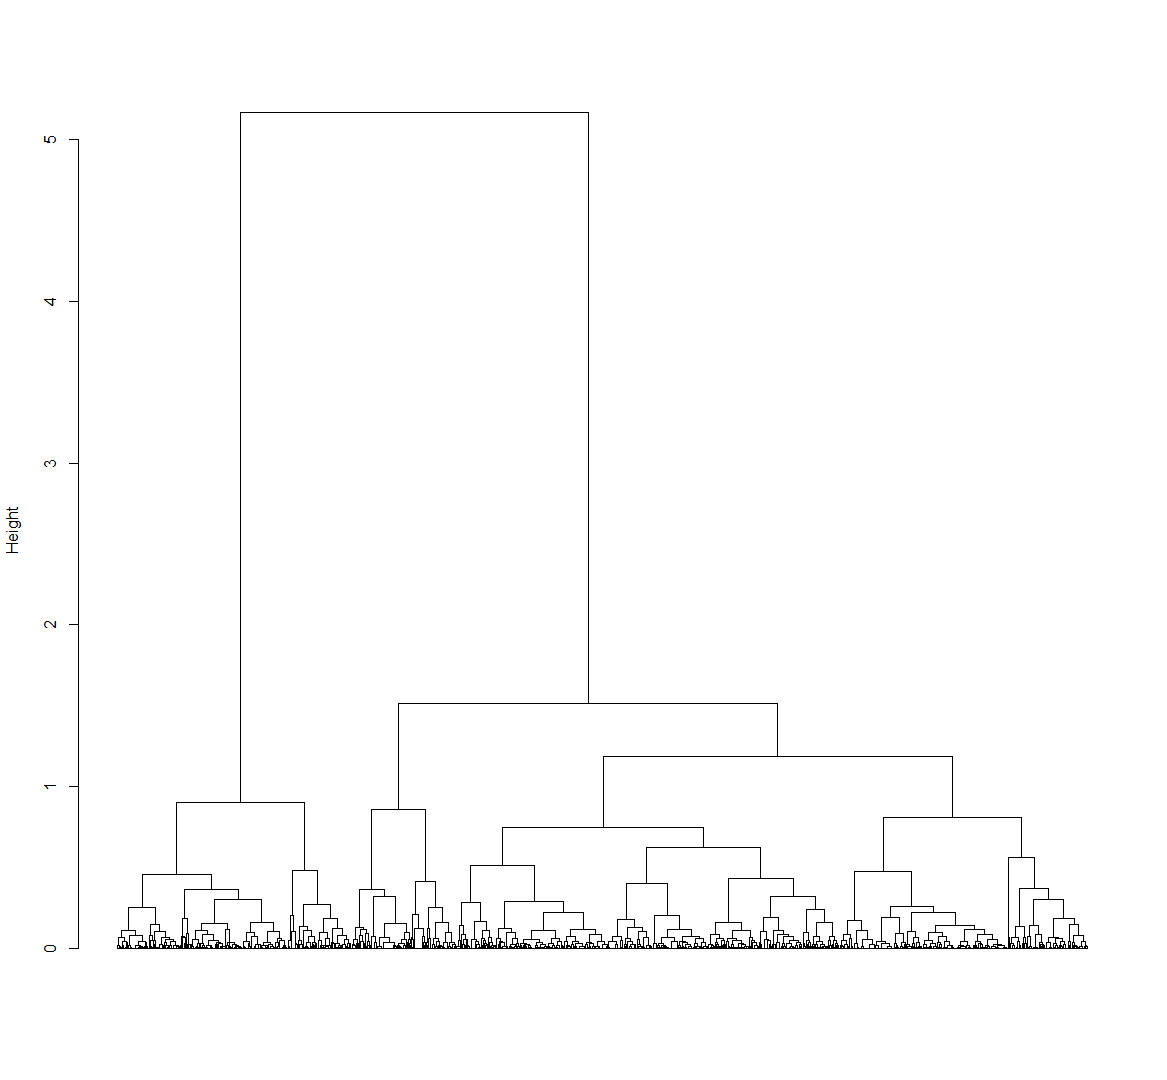
\includegraphics[width=0.8\textwidth]{Images/3_Preprocessing/mimmidend.png}
    \caption{Dendrograma usat pel MIMMI}
    \label{fig:Preprocessing_mimmi_dend}
\end{figure}

En aquest cas, vam escollir k = 4. Amb aquests clústers, realitzats amb les dades que no contenen missing data, es pot imputar la resta de instàncies simplement observant quin és el clúster que els hi pertoca i realitzant la mitja (o la moda, tot i que en aquest cas només s'han imputat variables numèriques).

\subsubsection{MICE} 
\textit{Multivariate Imputation by Chained Equations}, més conegut com MICE, és un altre mètode d'imputació. En aquest, es produeixen múltiples imputacions per variable que es combinen per obtenir el resultat final. Els paràmetres que es van usar per utilitzar-lo en la base de dades van ser: \textit{predictive mean matching} com a mètode (pmm), m (número de imputacions múltiples) 5 i màxim 5 iteracions.

R disposa d'un paquet amb aquest mètode, o sigui que la implementació ja estava feta.

\subsubsection{KNN}

Per imputar les dades usant KNN, s'han utilitzat tan sols les variables numèriques. S'han usat les variables completes (\textit{track\_popularity, album\_popularity, artist\_popularity, artist\_num, energy, loudness, acousticness, liveness, valence, tempo} i \textit{streams}) com a referència.

Per poder imputar, s'han usat com a train les instàncies del dataset amb aquestes variables on el dataset original no contenia missings a la variable a imputar. La "classificació" d'aquest train eren els valors de la variable a imputar (que no tenien missing). Llavors, com a test, s'usen la resta, que són els que contenen missing. D'aquesta manera es poden afegir aquests valors mancants usant el KNN. El valor de k usat ha estat el per defecte, 1, i la distància euclidiana (també el valor per defecte).

Després de les 3 imputacions, la suma total dels valors mancants del dataset era 420. Aquests, però, corresponen a valors mancants en les variables categòriques, especialment en aquelles provinents de APIs ja que va haver-hi alguns problemes. Més endavant s'explicarà com es van sol·lucionar aquests errors.


\subsection{Anàlisi descriptiva post processat}

% Anàlisi, dir quin vam escollir i per què

\subsection{Ampliació de la base de dades mitjançants APIs}

Com ja s'ha mencionat anteriorment, la nostra base de dades originària de \textbf{Kaggle} incloïa diverses variables sobre cançons com ara la seva llargada, timbre, duració, etc. Després d'un primer preprocessament on es van eliminar totes les aparicions de les cançons si l'artista no era el principal, ens vam centrar més en els artistes, ja que l'anàlisi resultava més interessant i prometedor. La falta d'informació detallada sobre els artistes ens va portar a utilitzar diferents APIs per a enriquir el nostre conjunt de dades.

\subsubsection{Selecció d'APIs}

Per a millorar la qualitat i riquesa de les dades, es va decidir incorporar informació addicional sobre els artistes, com ara la seva ubicació \textbf{(País / Ciutat)}, gènere \textbf{(Masculí / Femení / No binari)} i si l'artista és un \textbf{individu} o un \textbf{grup}. A més, també es va incorporar la lletra de les cançons per tal de poder realitzar un \textit{text analysis} més endavant.. Això es va aconseguir mitjançant l'ús de diverses APIs públiques:
\begin{itemize}
    \item \textbf{MusicBrainz API}: Per obtenir detalls específics dels artistes, incloent si són solistes o grups, i el gènere del grup basat en els seus membres.
    \item \textbf{CountriesNow API}: Per verificar si una ciutat determinada es troba dins d'un país específic, evitant així inconsistències en la ubicació.
    \item \textbf{RestCountries API}: Per obtenir la capital d'un país quan la ciutat de l'artista no està disponible o no es pot verificar correctament.
    \item \textbf{Genius API}: Per obtenir els lyrics de les cançons. S'ha usat amb la llibreria de \textit{Python} \textit{lyricsgenius} .
\end{itemize}

\subsubsection{Gestió d'errors i tècniques de millora}

Per a assegurar la fiabilitat i precisió de les dades recopilades, es van implementar diverses estratègies:
\begin{itemize}
    \item Esperar un temps prudencial entre trucades a la API per evitar sobrecàrregues i possibles bloquejos.
    \item Realitzar múltiples intents per cada trucada a l'API, gestionant els errors temporals de manera eficient.
    \item Substituir els valors no disponibles (\textit{NA}) per les capitals dels països corresponents quan la informació de la ciutat de l'artista no es trobava o era incorrecta.
    \item Verificació manual per a casos on les dades automàticament recollides no eren coherents, com ara ciutats que no pertanyien al país indicat o països erròniament identificats com a ciutats.
\end{itemize}

Malgrat l'aplicació d'aquestes mesures, alguns errors en la localització d'artistes van requerir correccions manuals, especialment en casos on les ciutats no concordaven amb els països o quan la informació retornada per les APIs era incorrecta a causa de la confusió amb altres artistes de nom similar. Aquestes situacions van ser poc freqüents però destacables, ja que reflecteixen les limitacions inherents a l'ús de dades automàticament recollides i la importància de la revisió humana en la curació de conjunts de dades.

\subsubsection{Resultats}

Després de l'execució de l'script i la implementació de les tècniques esmentades, es va obtenir un conjunt de dades considerablement millorat, amb informació més completa i precisa sobre els artistes i amb les lletres de les cançons. Aquest enriquiment de les dades obre noves possibilitats per a l'anàlisi, permetent estudis més detallats i específics sobre la música i els seus creadors en la plataforma Spotify.




%


\newpage

\section{Clústering avançat} 

En aquesta secció s'exploraran diferents tècniques avançades de clustering alhora que s'analitzaran i es compararan els resultats obtinguts. Cal mencionar en tots que els objectius de la creació de classes pot resultar diferent sobretot segons el mètode utilitza ja que, per exemple, en el \textit{K-modes} tan sols volem formar clústers per variables categòriques o en el \textit{time series clustering} volem agrupar instàncies de cançons segons una sola variable al llarg del temps.

\subsection{Clústering jeràrquic} \label{section:clustering_jerarquic3}

El clustering jeràrquic és un mètode d'agrupament de dades que no requereix donar-li el nombre de grups com a paràmetre, ja que es representa amb dendrograma (que mostra la relació de similitud entre els elements) i a partir d'allà es pot escollir la k. Aquest mètode ja es va explorar el quatrimetre passat.

En aquest apartat es fa un clústering jeràrquic però afegint les noves variables creades durant el preprocessament de les dades per veure de quina manera aquestes variables afecten a aquest agrupament. A l'agrupament les variables que no han estat incluides han estat week\_index i day\_release ja que s'ha considerat que es feient millor els clústers sense afegir-les. Tampoc s'han incluit les variables track\_id, track\_name, album\_name i artist\_name. 

% Foto del dendrograma sense pintar
\begin{figure}[H]
    \centering
    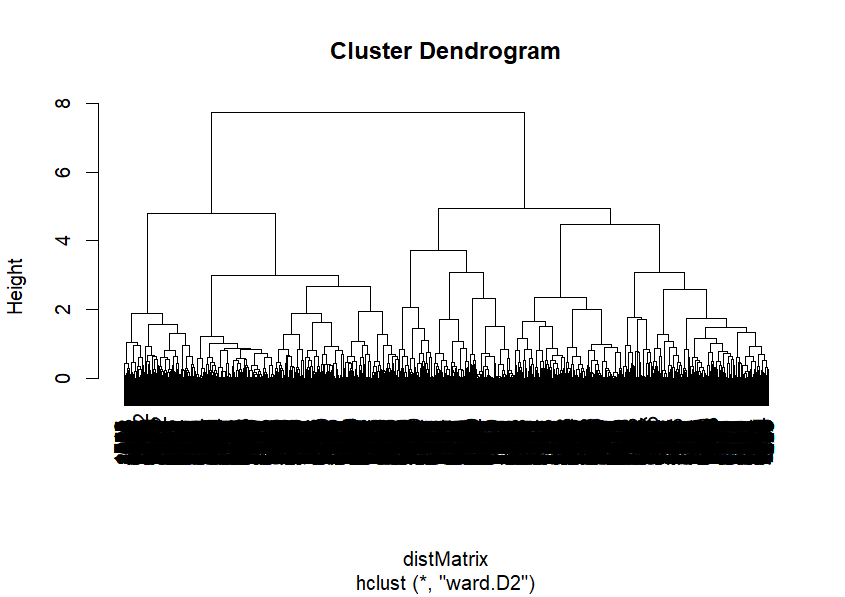
\includegraphics[width=0.8\textwidth]{Images/4_clustering/herarchical/dendogram.png}
    \caption{Dendrograma del clustering jeràrquic}
    \label{fig:dendogram}
\end{figure}

Observant el dendrograma, podem veure que es podria dividir entre dues classes, però per fer el profiling considerem que és millor agafar més classes. L'han passat vam triar 4 clústers, però en el cas d'ara ens quedarien les classes poc balancejades. Per això, triem 5 clústers.  

Amb el dendrograma resultant, es divideixen els 5 clústers de la següent manera: 

\begin{figure}[H]
    \centering
    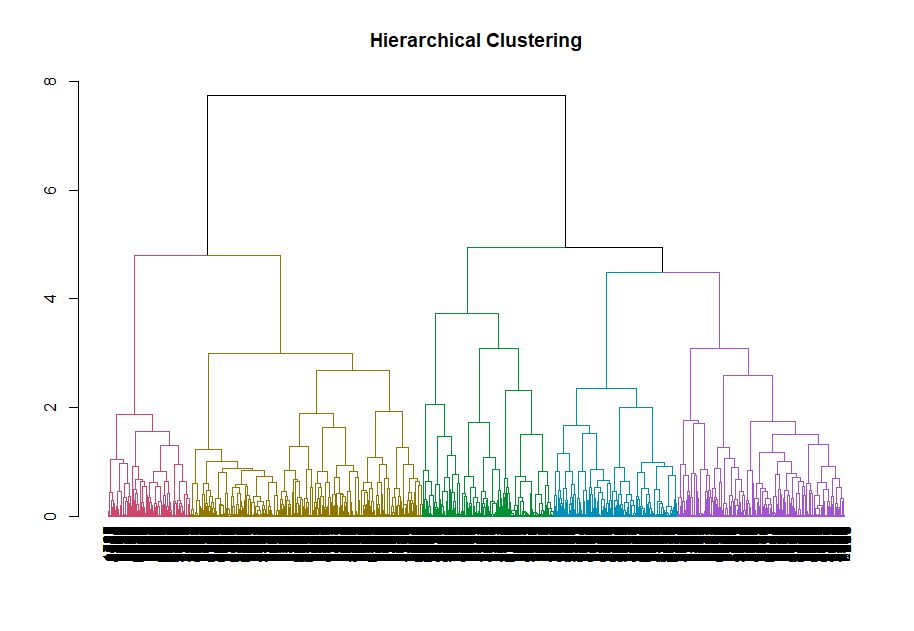
\includegraphics[width=0.8\textwidth]{Images/4_clustering/herarchical/hierarchical_dendogram_colors2.png}
    \caption{Dendrograma del clustering jeràrquic després de crear els clústers}
    \label{fig:hierarchical_dendogram_colors2}
\end{figure}

Abans de realitzar el profiling del clústering jeràrquic, s'ha realitzat un PCA per poder observar els clusters que s'han identificat en el clústering jeràrquic en les dos primeres components principals.

\begin{figure}[H]
    \centering
    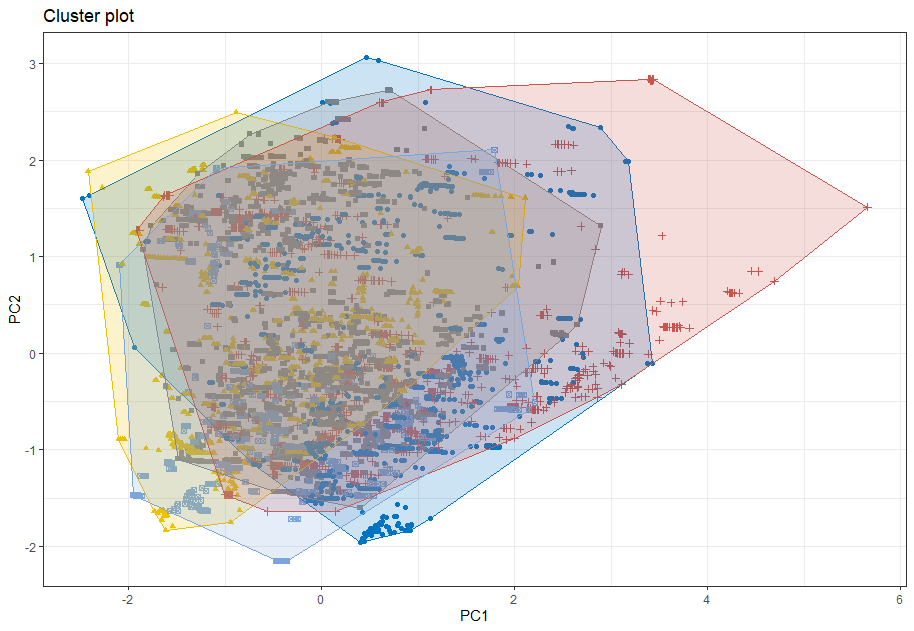
\includegraphics[width=0.7\textwidth]{Images/4_clustering/herarchical/pca_hierarchical.png}
    \caption{Resultats del clústering jerarquic}
    \label{fig:pca_hierarchical}
\end{figure}

Com es pot observar, tenim 5 clústers, uns semblen més dispersos i altres més densos indicant variacions en la cohesió interna dels grups. Tot i així, és important recalcar que les dos primeres components no capturen una gran informació de les dades (17\% el primer component i 14\% el segon).

Encara que no es pot observar una clara divisió dels clústers degut al baix percentatge de variància explicada en les dos primeres components, amb  el profiling que s'ha realitzat posteriorment, s'examinarà les dades en la seva totalitat i les característiques de cada clúster.   

La mida dels clústers finals és de:
\begin{table}[H]
\centering
\begin{tabular}{|c|c|c|c|c|}
\hline
1    & 2    & 3   & 4   & 5 \\ \hline
1574 & 1997 & 2785 & 1489  & 990  \\ \hline
\end{tabular}
\caption{Resultat del clústering jerarquic}
\label{tab:clustering_results}
\end{table}

Es pot veure que l'últim clúster té una mida més petita que la resta, tot i així, la mida de tots els clústers és bastant similar.

\subsection{K-modes}

El K-modes és un algoritme de clustering i és una extensió del k-means, un algoritme que ja hem treballat en aquesta assignatura. L'algorisme fa bàsicament el mateix però en comptes d'utilitzar dades numèriques, utilitza exclusivament dades categòriques. En el nostre cas hem seleccionat totes les variables categòriques que ja teniem ("pop","hip\_hop", "collab","rank\_group"...) i a més les noves variables afegides durant el preprocessament ("gender", "is\_group", "nationality",\"city"). La variable lyrics no s'ha inclòs en el clustering.

Divideix les dades en un nombre k de grups basant-se en la similitud entre ells. La k, com al k-means, és un hiperparàmetre que hem de triar nosaltres. Per veure la similitud de les dades, en comptes d'utilitzar la distància euclidiana, utilitzem una mesura de disimilitud per a dades categòriques.

Utilitzant el paquet klaR en R, hem fet servir kmodes() donant-li el hiperparàmetre k = 4. Com no es poden utilitzar mètriques de validació per les variables categòriques, s'ha triat la k no agafant un nombre molt gran, i a partir del clustering jeràrquic que vam fer l'any passat. 

Un cop s'ha realitzat el K-Modes, s'ha realitzat un Anàlisi dels Components Principals (ACP) per visualitzar la distribució dels clústers respecte les variables numèriques. No s'ha observat una classificació clara de les variables numèriques en els clústers realitzats amb les variables categòriques. Tot i així, en la cinquena i sisena dimensió (8,5\% i 6\% de variància explicada respectivament) si que s'observa una petita separació entre clústers.  \\

\begin{figure}[H]
    \centering
    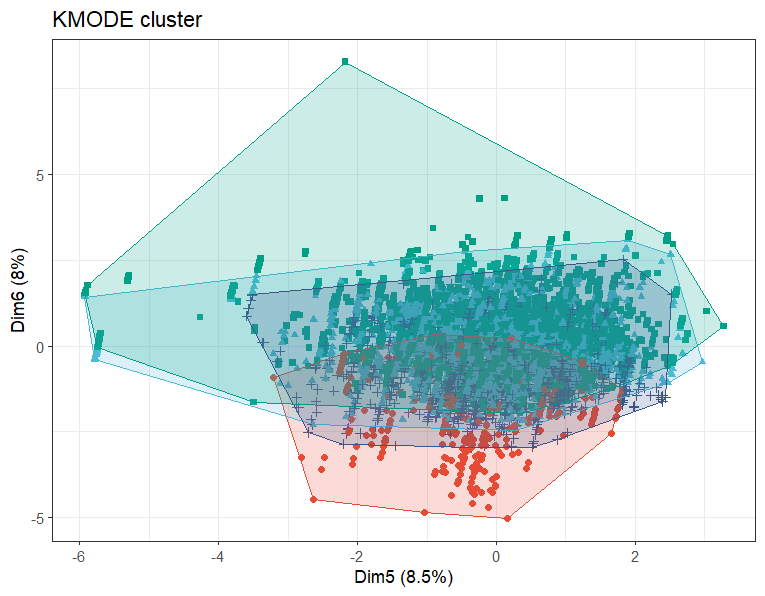
\includegraphics[width=0.7\textwidth]{Images/4_clustering/KMODES/kmodes1.png}
    \caption{Resultats del K-Modes en la 5ª i 6ª dimensió}
    \label{fig:kmodes1}
\end{figure}

La dimensió 5 està relacionada amb l'speechines i el tempo d'una cançó i la dimensió 6 està més relacionada amb el número d'artistes, la duració i la danceability d'una cançó. Per tant, es podria indicar que el K-Means divideix els clústers segons aquestes característiques. Tot i així, cal recalcar que aquestes dimensions només expliquen un 16\% de la variància total de les dades, per tant, caldria fer el profiling per poder afirmar aquesta conclusió.

\begin{figure}[H]
    \centering
    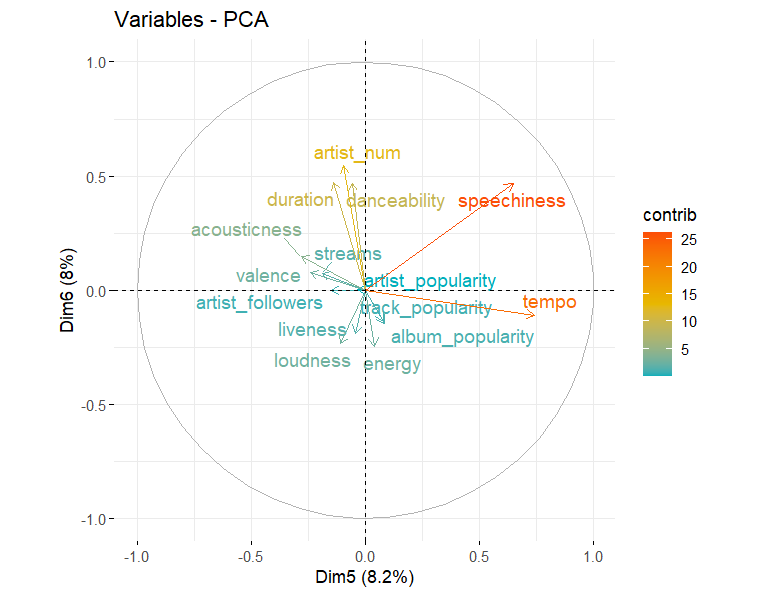
\includegraphics[width=0.7\textwidth]{Images/4_clustering/KMODES/kmodes2.png}
    \caption{Variables i la seva contribució en el 5é i 6é components principals}
    \label{fig:kmodes2}
\end{figure}

Un cop fet ja s'ha experimentat amb el k-means i amb el k-modas, s'ha trobat interessant  fer ús del k-prototypes. Aquesta és una tècnica que barreja les variables numèriques i categòriques. S'ha utilitzat la funció kproto() de clustMixType per fer el clustering. Com amb el k-means, basant-nos en els resultats de l'últim agrupament, s'ha utilitzat el número de clústers k=4. També s'han afegit més paràmetres. El paràmetre lambda s'encarrega d'equilibrar la importància entre els dos tipus de variales, també hem posat un màxim d'iteracions i el nombre d'ejecucions a fer amb diferents centroides inicials (nstart). 

\subsection{CURE}
Clustering Using REpresentatives (\ref{guha_1998_cure}) és una tècnica avançada de clústering centrada en millorar el rendiment d’aquest tipus d’algorismes per bases de dades especialment grans. Es basa en el concepte de trobar uns punts representatius inicials i realitzar el clústering amb aquests. Un cop es troben uns centroides adequats, es calculen les distàncies de la resta dels punts a aquests i s’escull el millor.

S’ha escollit realitzar-lo usant tant les variables numèriques com algunes categòriques (gèneres...). Per tal de poder combinar aquestes variables mixtes, les categòriques s’han transformat prèviament en one-hot-encoding. A més, per evitar problemes amb les magnituds (algunes numèriques tenien valors entre 0 i 1 mentres que d’altres arribaven als milions), les variables numèriques s’han escalat usant la funció scale de R.

\begin{figure}[H]
    \centering
    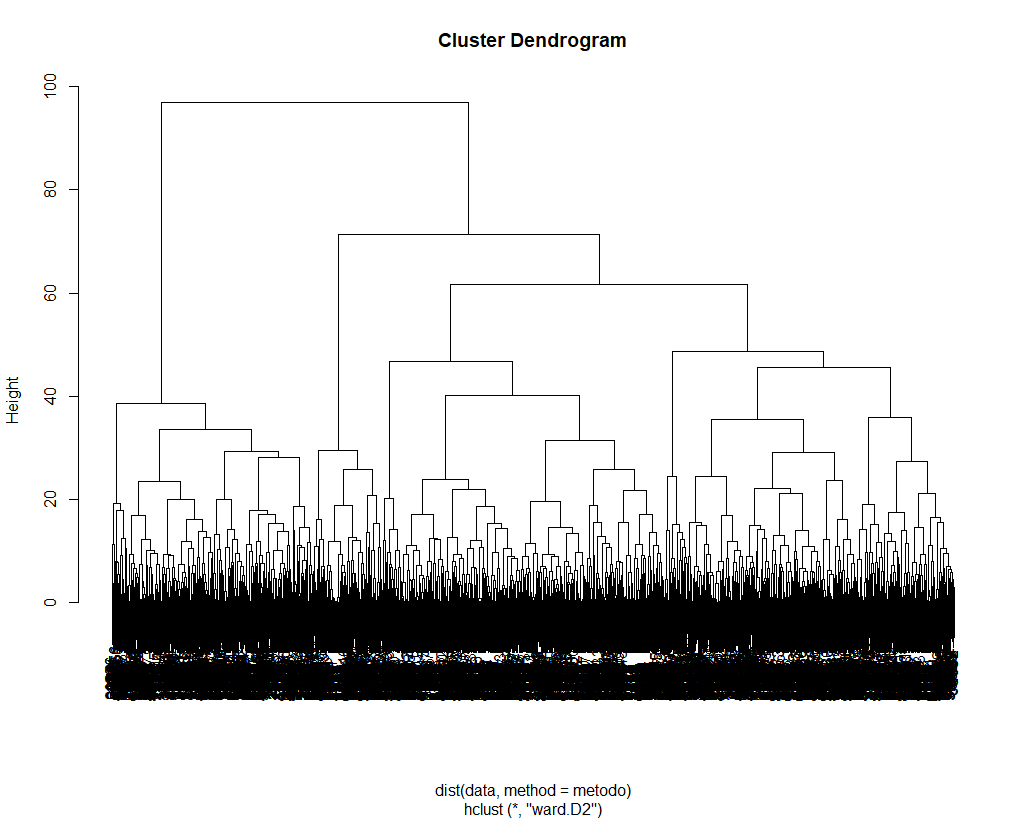
\includegraphics[width=0.8\textwidth]{Images/4_clustering/CURE/curedendrogram.png}
    \caption{Dendrograma de les dades usades pel CURE (jeràrquic, amb ward D2)}
    \label{fig:CURE_dend}
\end{figure}

La distància usada ha estat la euclidiana, ja que després d’aquest petit processat de les dades es podia utilitzar. Amb un  clústering jeràrquic inicial s’ha observat que un bon punt de tall era 4 observant la figura \ref{fig:CURE_dend}, i per tant s’ha escollit aquesta k. La r escollida, és a dir, el percentatge de representatius, ha estat 0.25.

Els 4 clústers dels representatius han quedat amb el següent nombre de cançons en cada un (taula \ref{tab:CURE_taularep}):

\begin{table}[H]
\centering
\begin{tabular}{lllll}
\cline{1-4}
\multicolumn{1}{|c|}{1}   & \multicolumn{1}{c|}{2}   & \multicolumn{1}{c|}{3}    & \multicolumn{1}{c|}{4}   &  \\ \cline{1-4}
\multicolumn{1}{|c|}{653} & \multicolumn{1}{c|}{654} & \multicolumn{1}{c|}{1211} & \multicolumn{1}{c|}{133} &  \\ \cline{1-4}
                          &                          &                           &                          &  \\
                          &                          &                           &                          & 
\end{tabular}
\caption{Resultat del clústering dels representatius}
\label{tab:CURE_taularep}
\end{table}

A partir d’aquests, es poden assignar clústers a la resta de dades. El resultat es pot observar a \ref{tab:CURE_taulanorep}.

\begin{table}[H]
\centering
\begin{tabular}{lllll}
\cline{1-4}
\multicolumn{1}{|c|}{1}    & \multicolumn{1}{c|}{2}    & \multicolumn{1}{c|}{3}   & \multicolumn{1}{c|}{4}   &  \\ \cline{1-4}
\multicolumn{1}{|c|}{3266} & \multicolumn{1}{c|}{1939} & \multicolumn{1}{c|}{670} & \multicolumn{1}{c|}{309} &  \\ \cline{1-4}
                           &                           &                          &                          &  \\
                           &                           &                          &                          & 
\end{tabular}
\caption{Resultat del clústering dels no representatius}
\label{tab:CURE_taulanorep}
\end{table}

Observem com han quedat lleugerament desbalancejats. Se’ns presenta un grup 1 amb moltes de les instàncies, seguit d'un grup 2 que també en té moltes. D'altra banda, els clústers 3 i 4 tenen pocs elements (tot i que el 3 té molts representatius). Els resultats d'aquest clústering es poden visualitzar usant les dues primeres dimensions del PCA, com es pot observar a la figura \ref{fig:CURE_res}.

\begin{figure}[H]
    \centering
    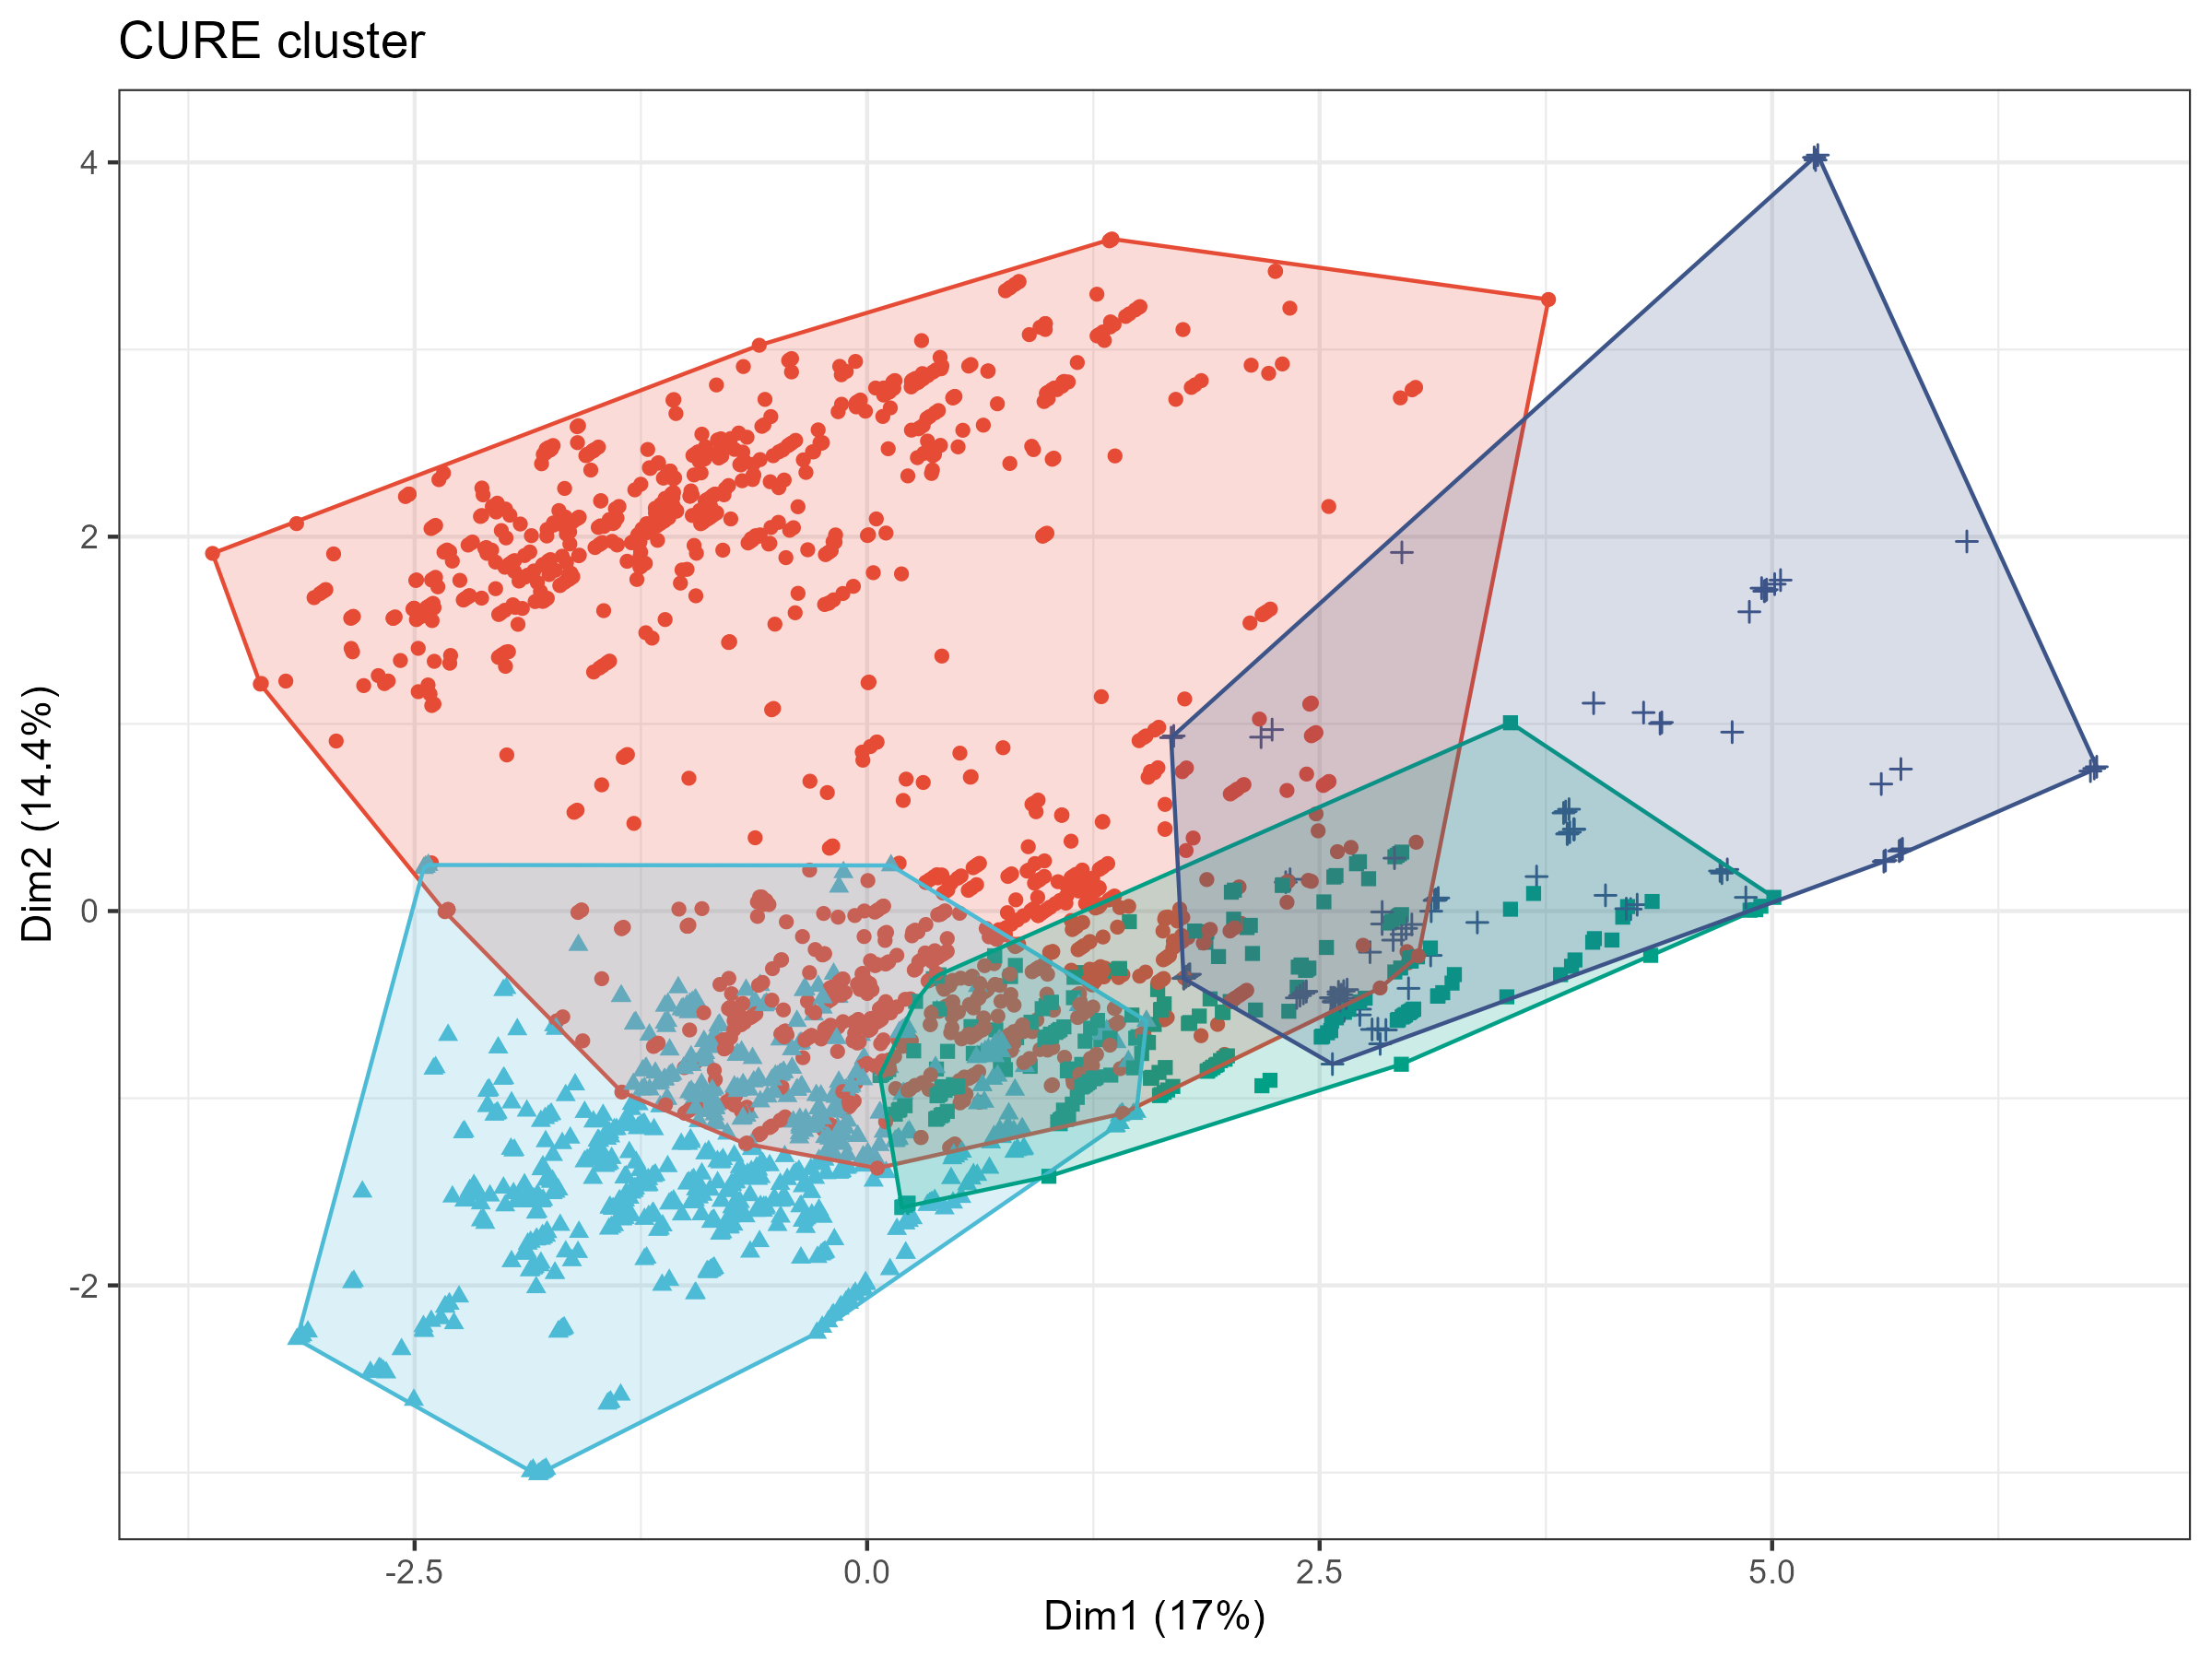
\includegraphics[width=0.8\textwidth]{Images/4_clustering/CURE/cure.png}
    \caption{Resultats del clústering usant CURE (4,0.15)}
    \label{fig:CURE_res}
\end{figure}

S'observa un gran clúster vermell, corresponent probablement al clúster 1. Aquest ocupa un núvol de punts situat a l'espai superior, així com la part central del núvol inferior. Amb valors negatius tant de la primera com de la segona dimensió trobem el clúster blau clar, corresponent al número 2, que és el segon més gran. Finalment, el clúster verd es situa al centre del núvol inferior, amb valors de la dimensió 2 bastant baixos, i el clúster 4, de color blau fosc, és el que engloba els punts amb valors més alts de la dimensió 1.

\subsection{DBSCAN}

El DBSCAN (\cite{dbscan}) és una tècnica de clústering basada en densitat. Per tal de poder observar millor com es reparteixen les nostres dades en aquest aspecte, el primer pas realitzat ha sigut un anàlisi dels components principals (PCA) (figura \ref{fig:DBSCAN_pca}). Aquest, a diferència de l'any passat, no ha estat realitzat en profunditat: tan sols ha estat usat com a tècnica de visualització de dades.

\begin{figure}[H]
    \centering
    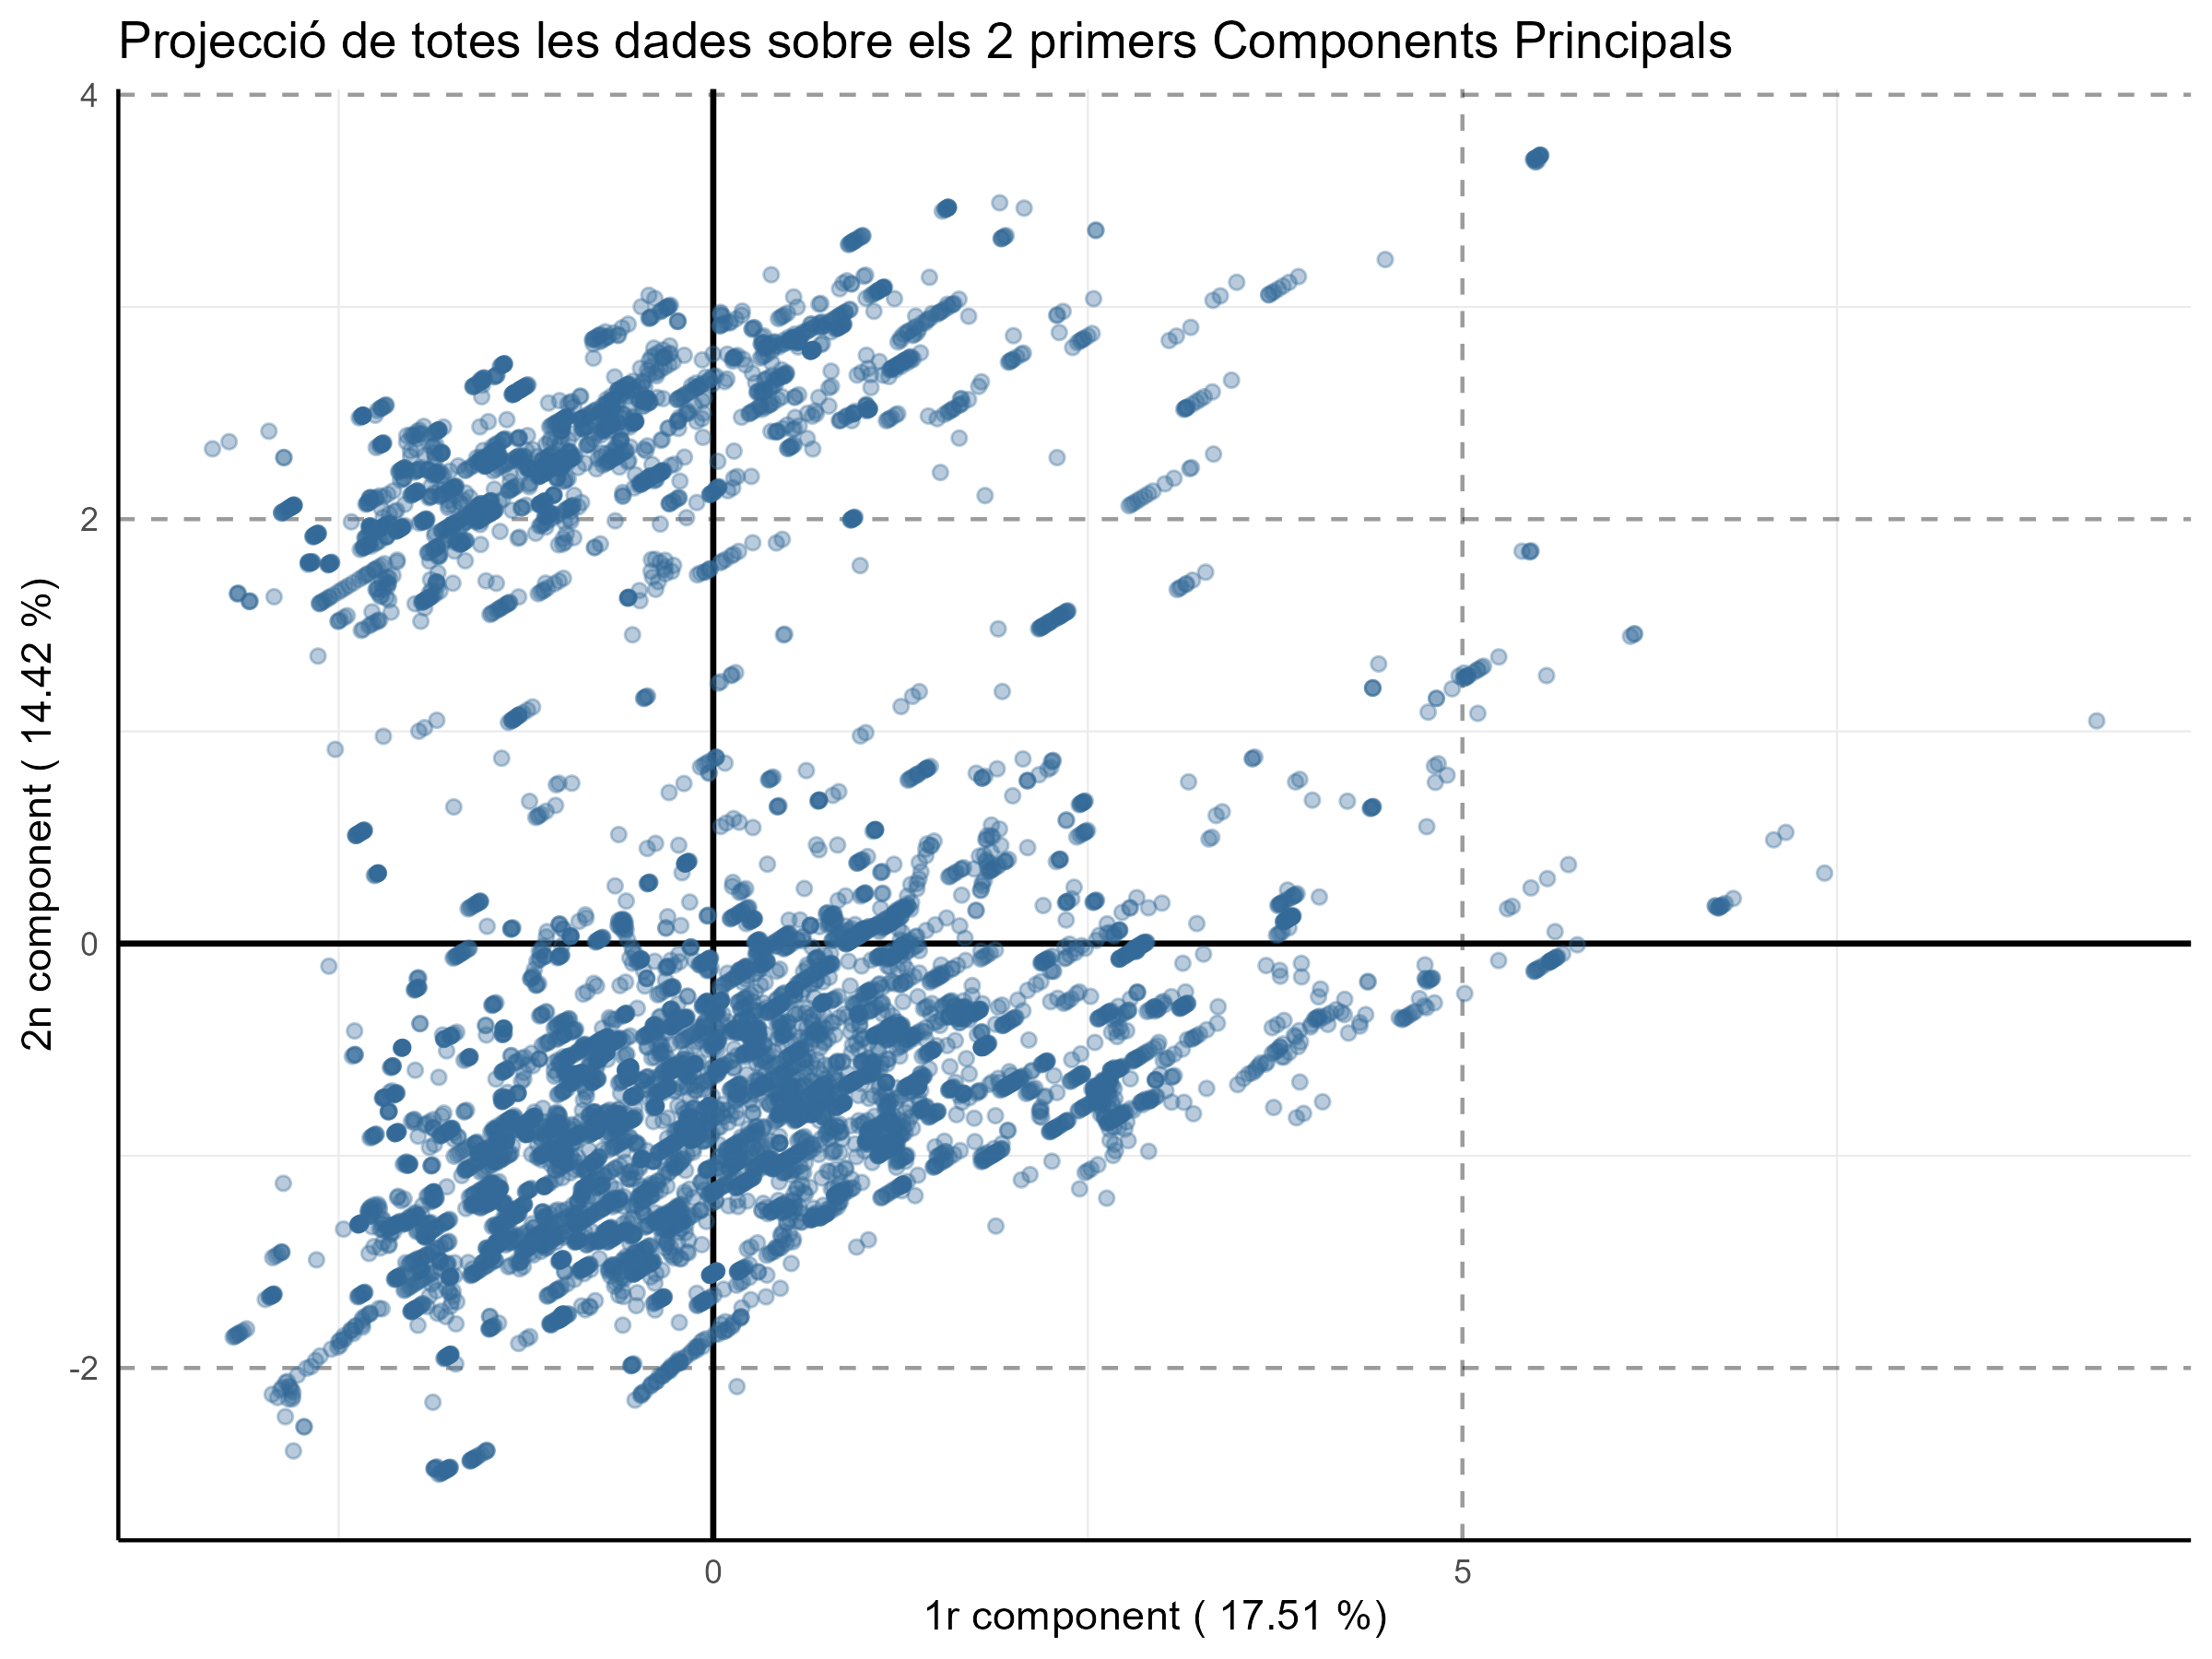
\includegraphics[width=0.8\textwidth]{Images/4_clustering/DBSCAN/dbscanpca.png}
    \caption{Dades descomposades en els dos primers components principals}
    \label{fig:DBSCAN_pca}
\end{figure}

A simple vista, basant-nos en les dues components principals, observem dos grans grups: un amb valors negatius de la segona component i un altre amb valors positius. Analitzant les variables que influeixen en aquests components (figura \ref{fig:DBSCAN_pca_contrib}), sembla ser que el grup inferior conté cançons més populars, mentres que l'altre conté cançons més antigues i per tant menys populars (Dimensió 2). La dimensió 1 ens indica com d'acústica o trista és la cançó: valors negatius indiquen cançó positiva, amb energia i forta (potent) mentre que valors positius indiquen una major \textit{acousticness}.

\begin{figure}[H]
    \centering
    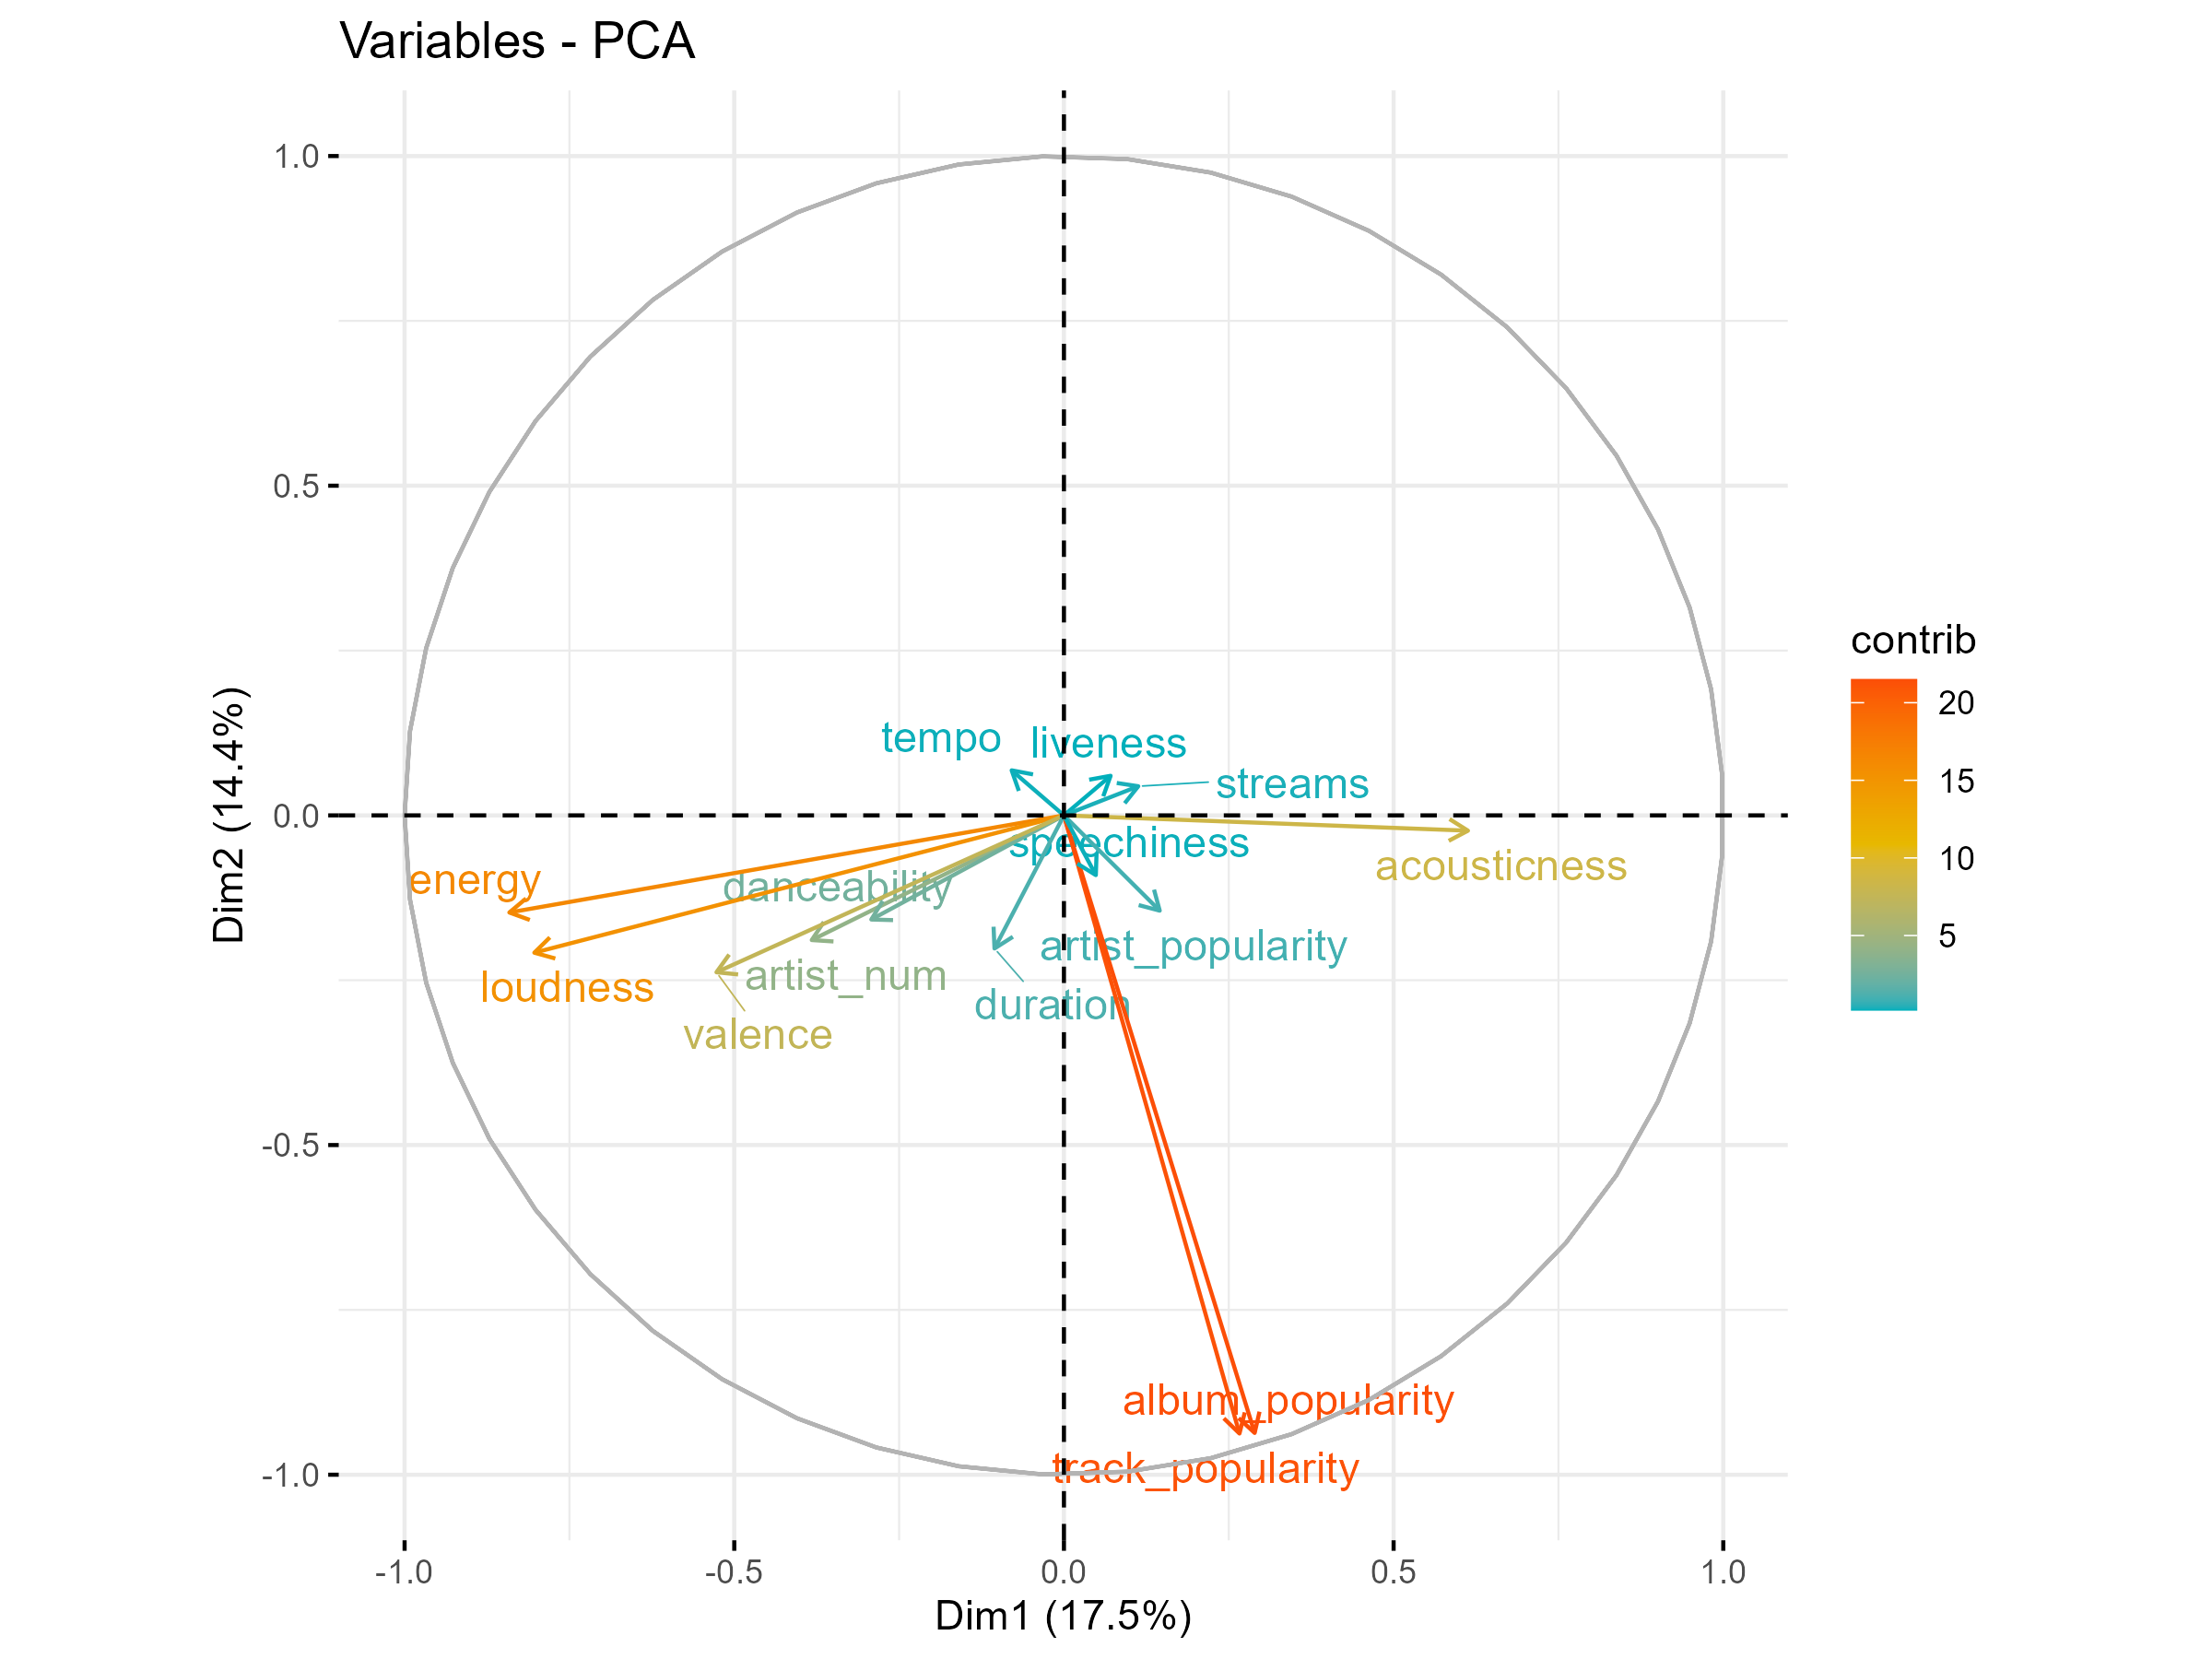
\includegraphics[width=0.8\textwidth]{Images/4_clustering/DBSCAN/dbscanpcacomponents.png}
    \caption{Variables i la seva contribució en cada un dels dos primers components principals.}
    \label{fig:DBSCAN_pca_contrib}
\end{figure}

Abans de realitzar el DBSCAN, el clústering basat en densitat, s’ha creat un petit k-means per tal d’observar la nostra distribució de dades  (figura \ref{fig:KMEANS}). En aquest cas, s’ha usat una k amb valor 5. Cal destacar que a partir d'aquest moment, usarem unes dades normalitzades ja que les distàncies (concretament, els rangs de valors de les variables) poden afectar a aquests clústers.

\begin{figure}[H]
    \centering
    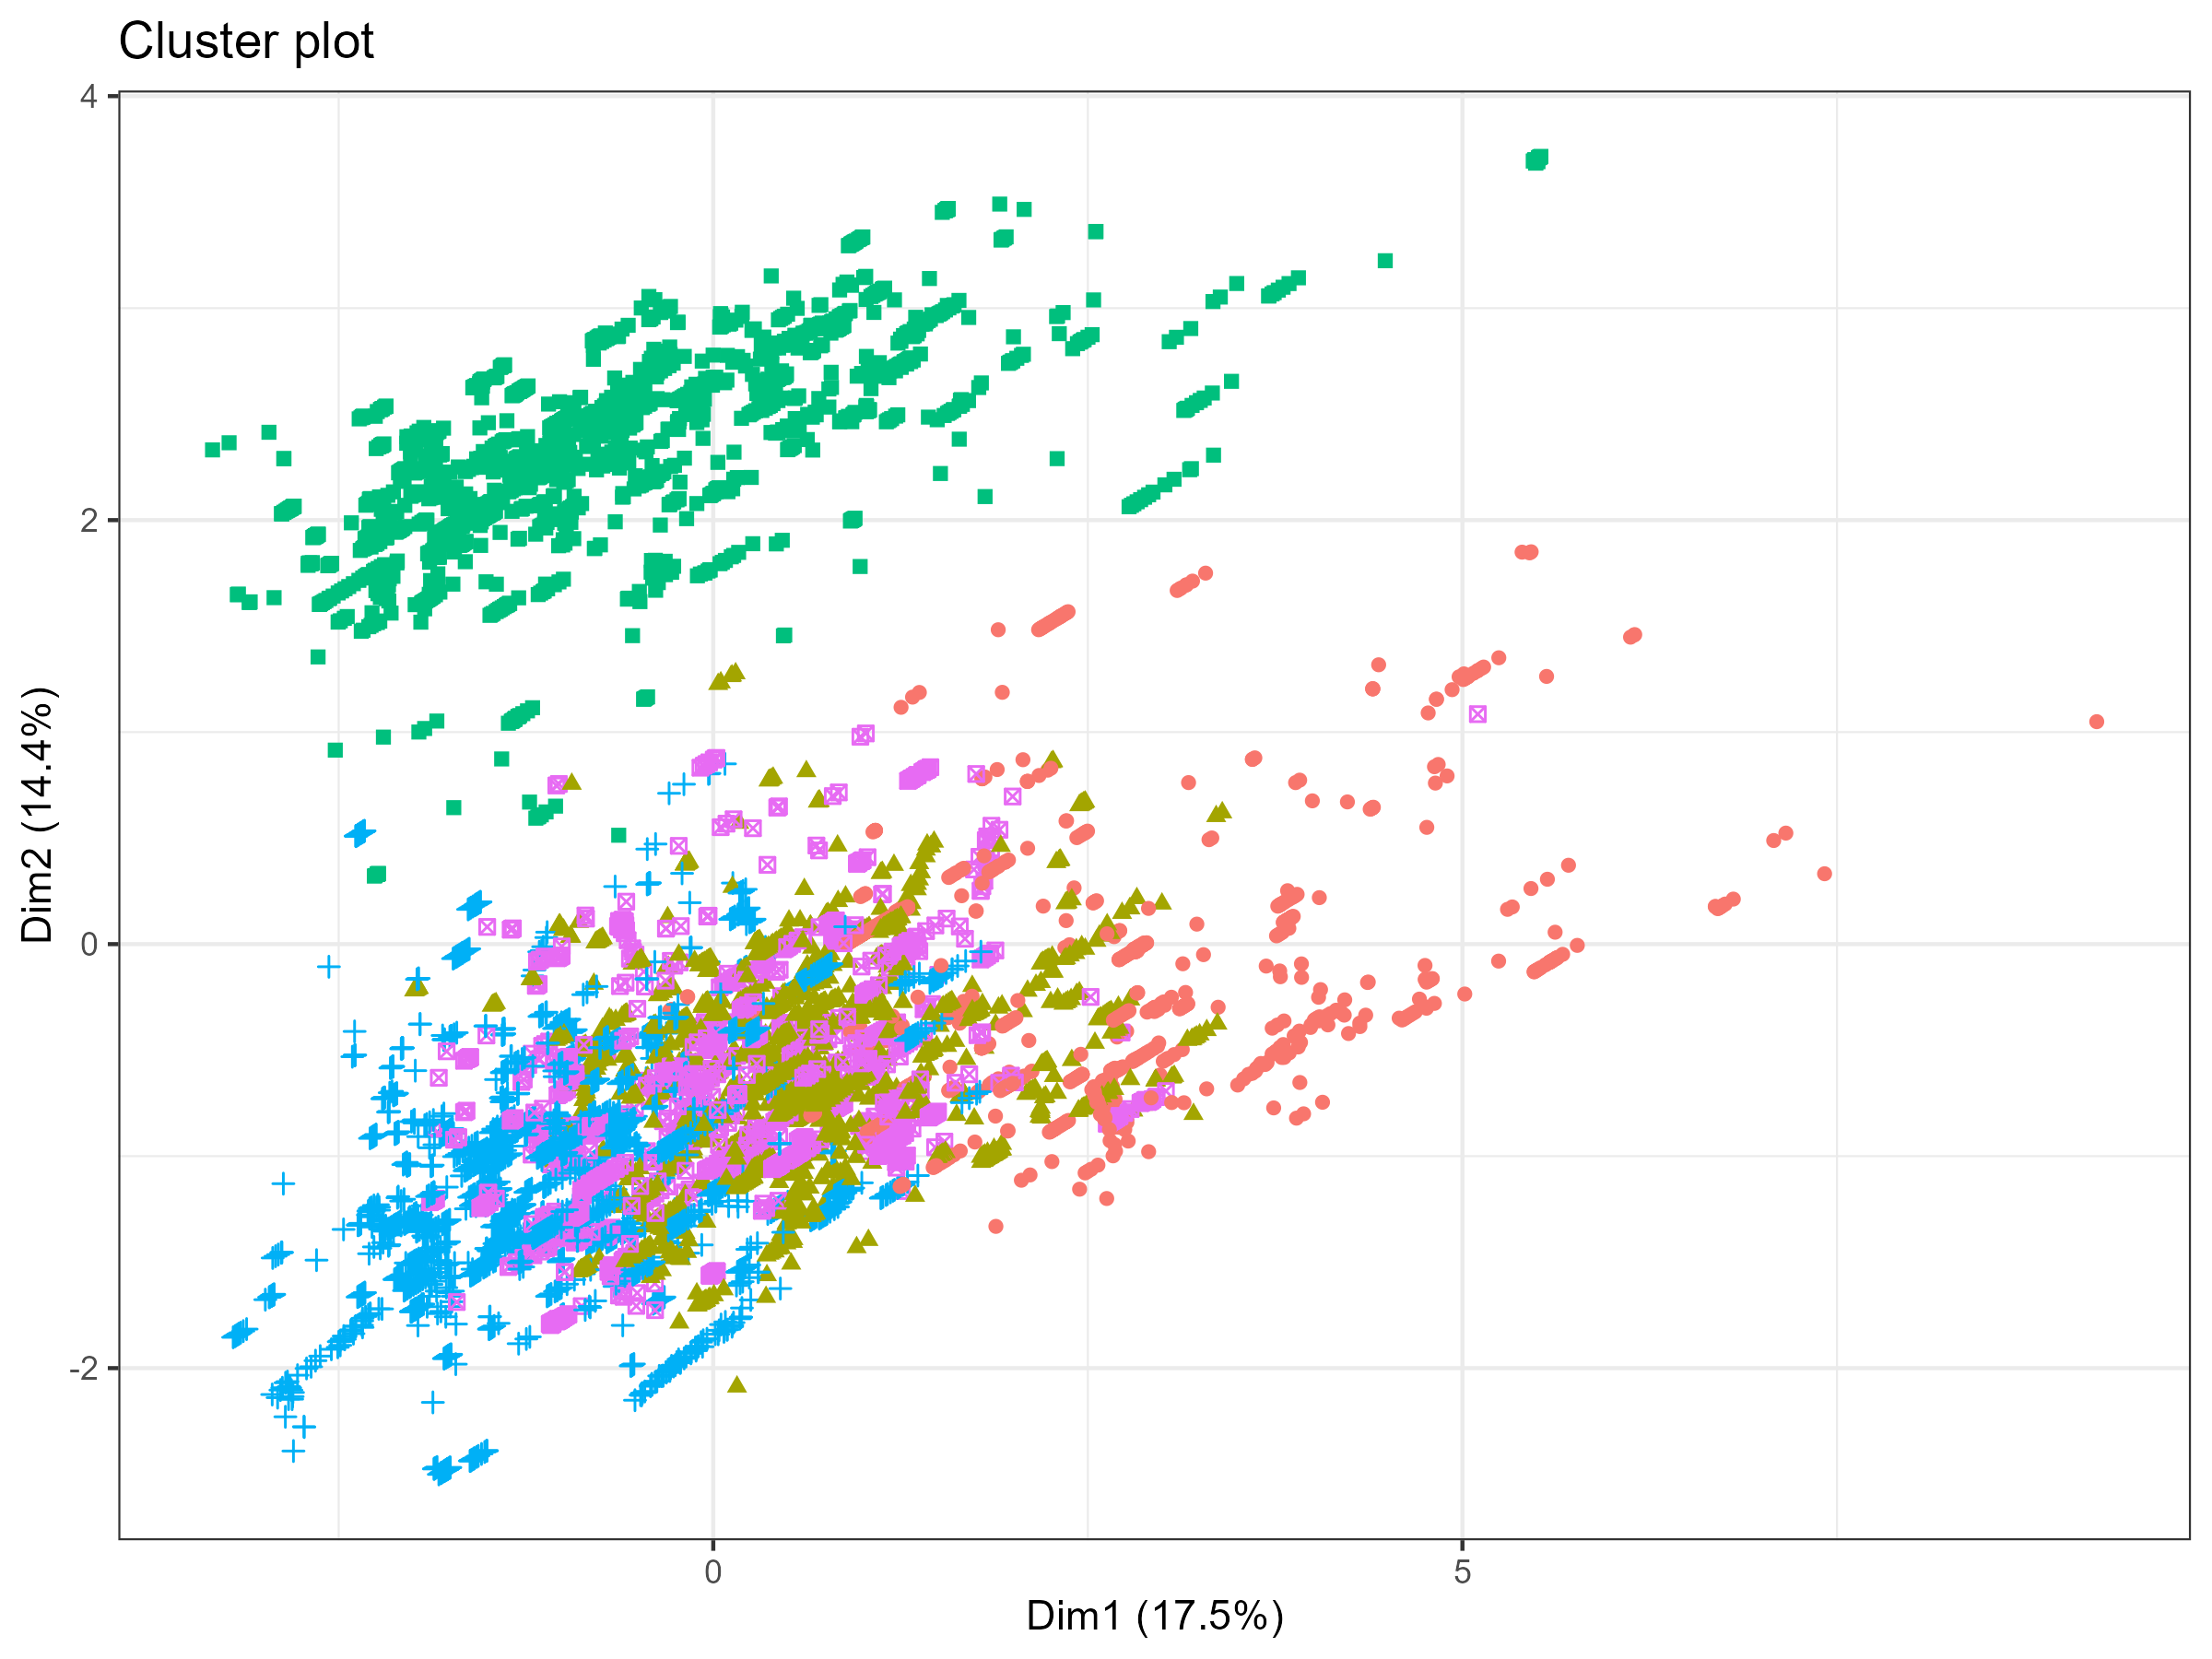
\includegraphics[width=0.8\textwidth]{Images/4_clustering/DBSCAN/kmeans.png}
    \caption{Resultats del clústering usant K-MEANS.}
    \label{fig:KMEANS}
\end{figure}

El grup superior, vist anteriorment, ha estat catalogat pràcticament de manera íntegra en el clúster verd. Pel que fa l’altre, s’ha repartit en funció de la dimensió 1: valors més baixos corresponen al clúster blau, els mitjanament baixos al violeta, els mitjanament alts a un verd més marronós i els alts a un taronja. Els dos clústers amb valors mitjos, el violeta i el marró, han quedat bastant barrejats. En general, però, els clústers creats són bastant bons, i ens serviran de referència per comparar amb els trobats pel DBSCAN.

Observant aquests mateixos clústers en la tercera i quarta dimensió (figura \ref{fig:KMEANS_34}), les dades queden molt més barrejades . Els clústers verds, taronja i marró queden completament inseparables, i els únics que podriem distingir serien el blau, amb valors negatius de la dimensió 3 i el lila amb valors positius. Mirant què representen les dimensions, sembla ser que separa les cançons més aviat llargues i ràpides (lila) contra les més ballables (blau).

\begin{figure}[H]
    \centering
    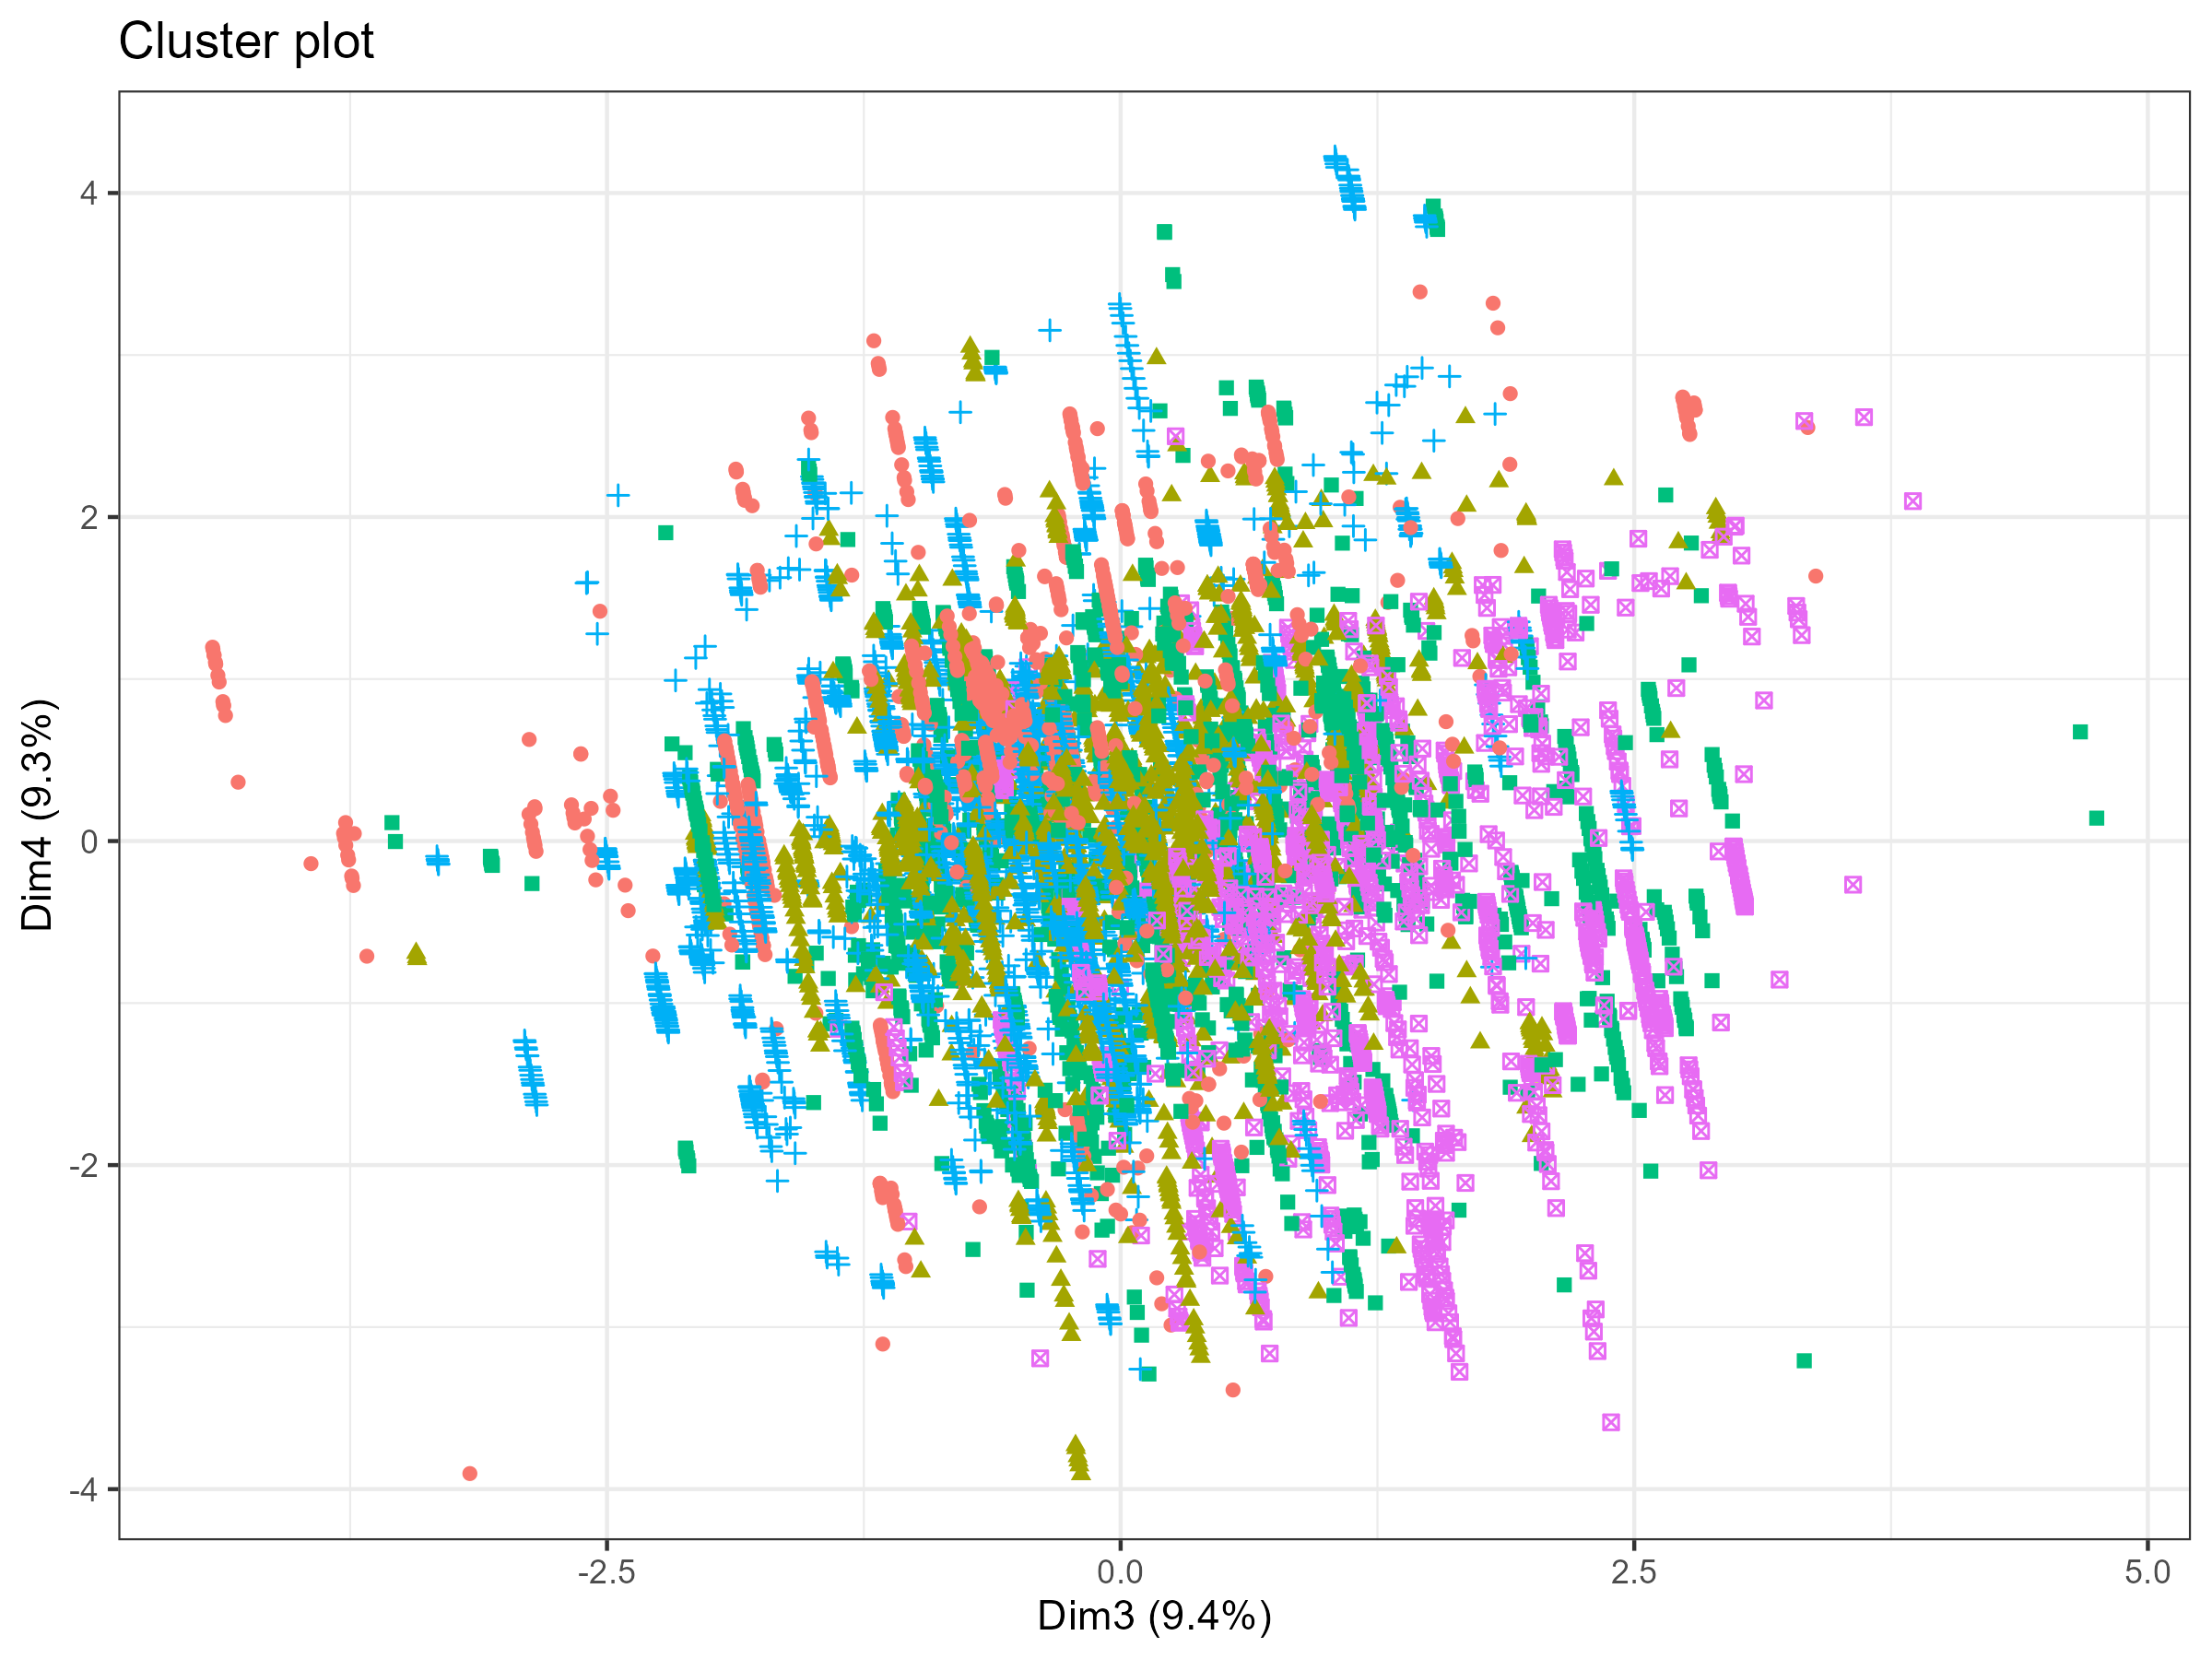
\includegraphics[width=0.8\textwidth]{Images/4_clustering/DBSCAN/kmeans34.png}
    \caption{Resultats del clústering usant K-MEANS visualitzats en components principals 3 i 4}
    \label{fig:KMEANS_34}
\end{figure}

Passant ja al DBSCAN, l’inicial (figura \ref{fig:DBSCAN_inicial}) realitzat amb 0.15 de espsilon i minPts 20 senyalava la gran majoria de punts com outliers, representats com a punts negres transparents. A més, creava molts clústers però molt petits (més de 100 clústers).

\begin{figure}[H]
    \centering
    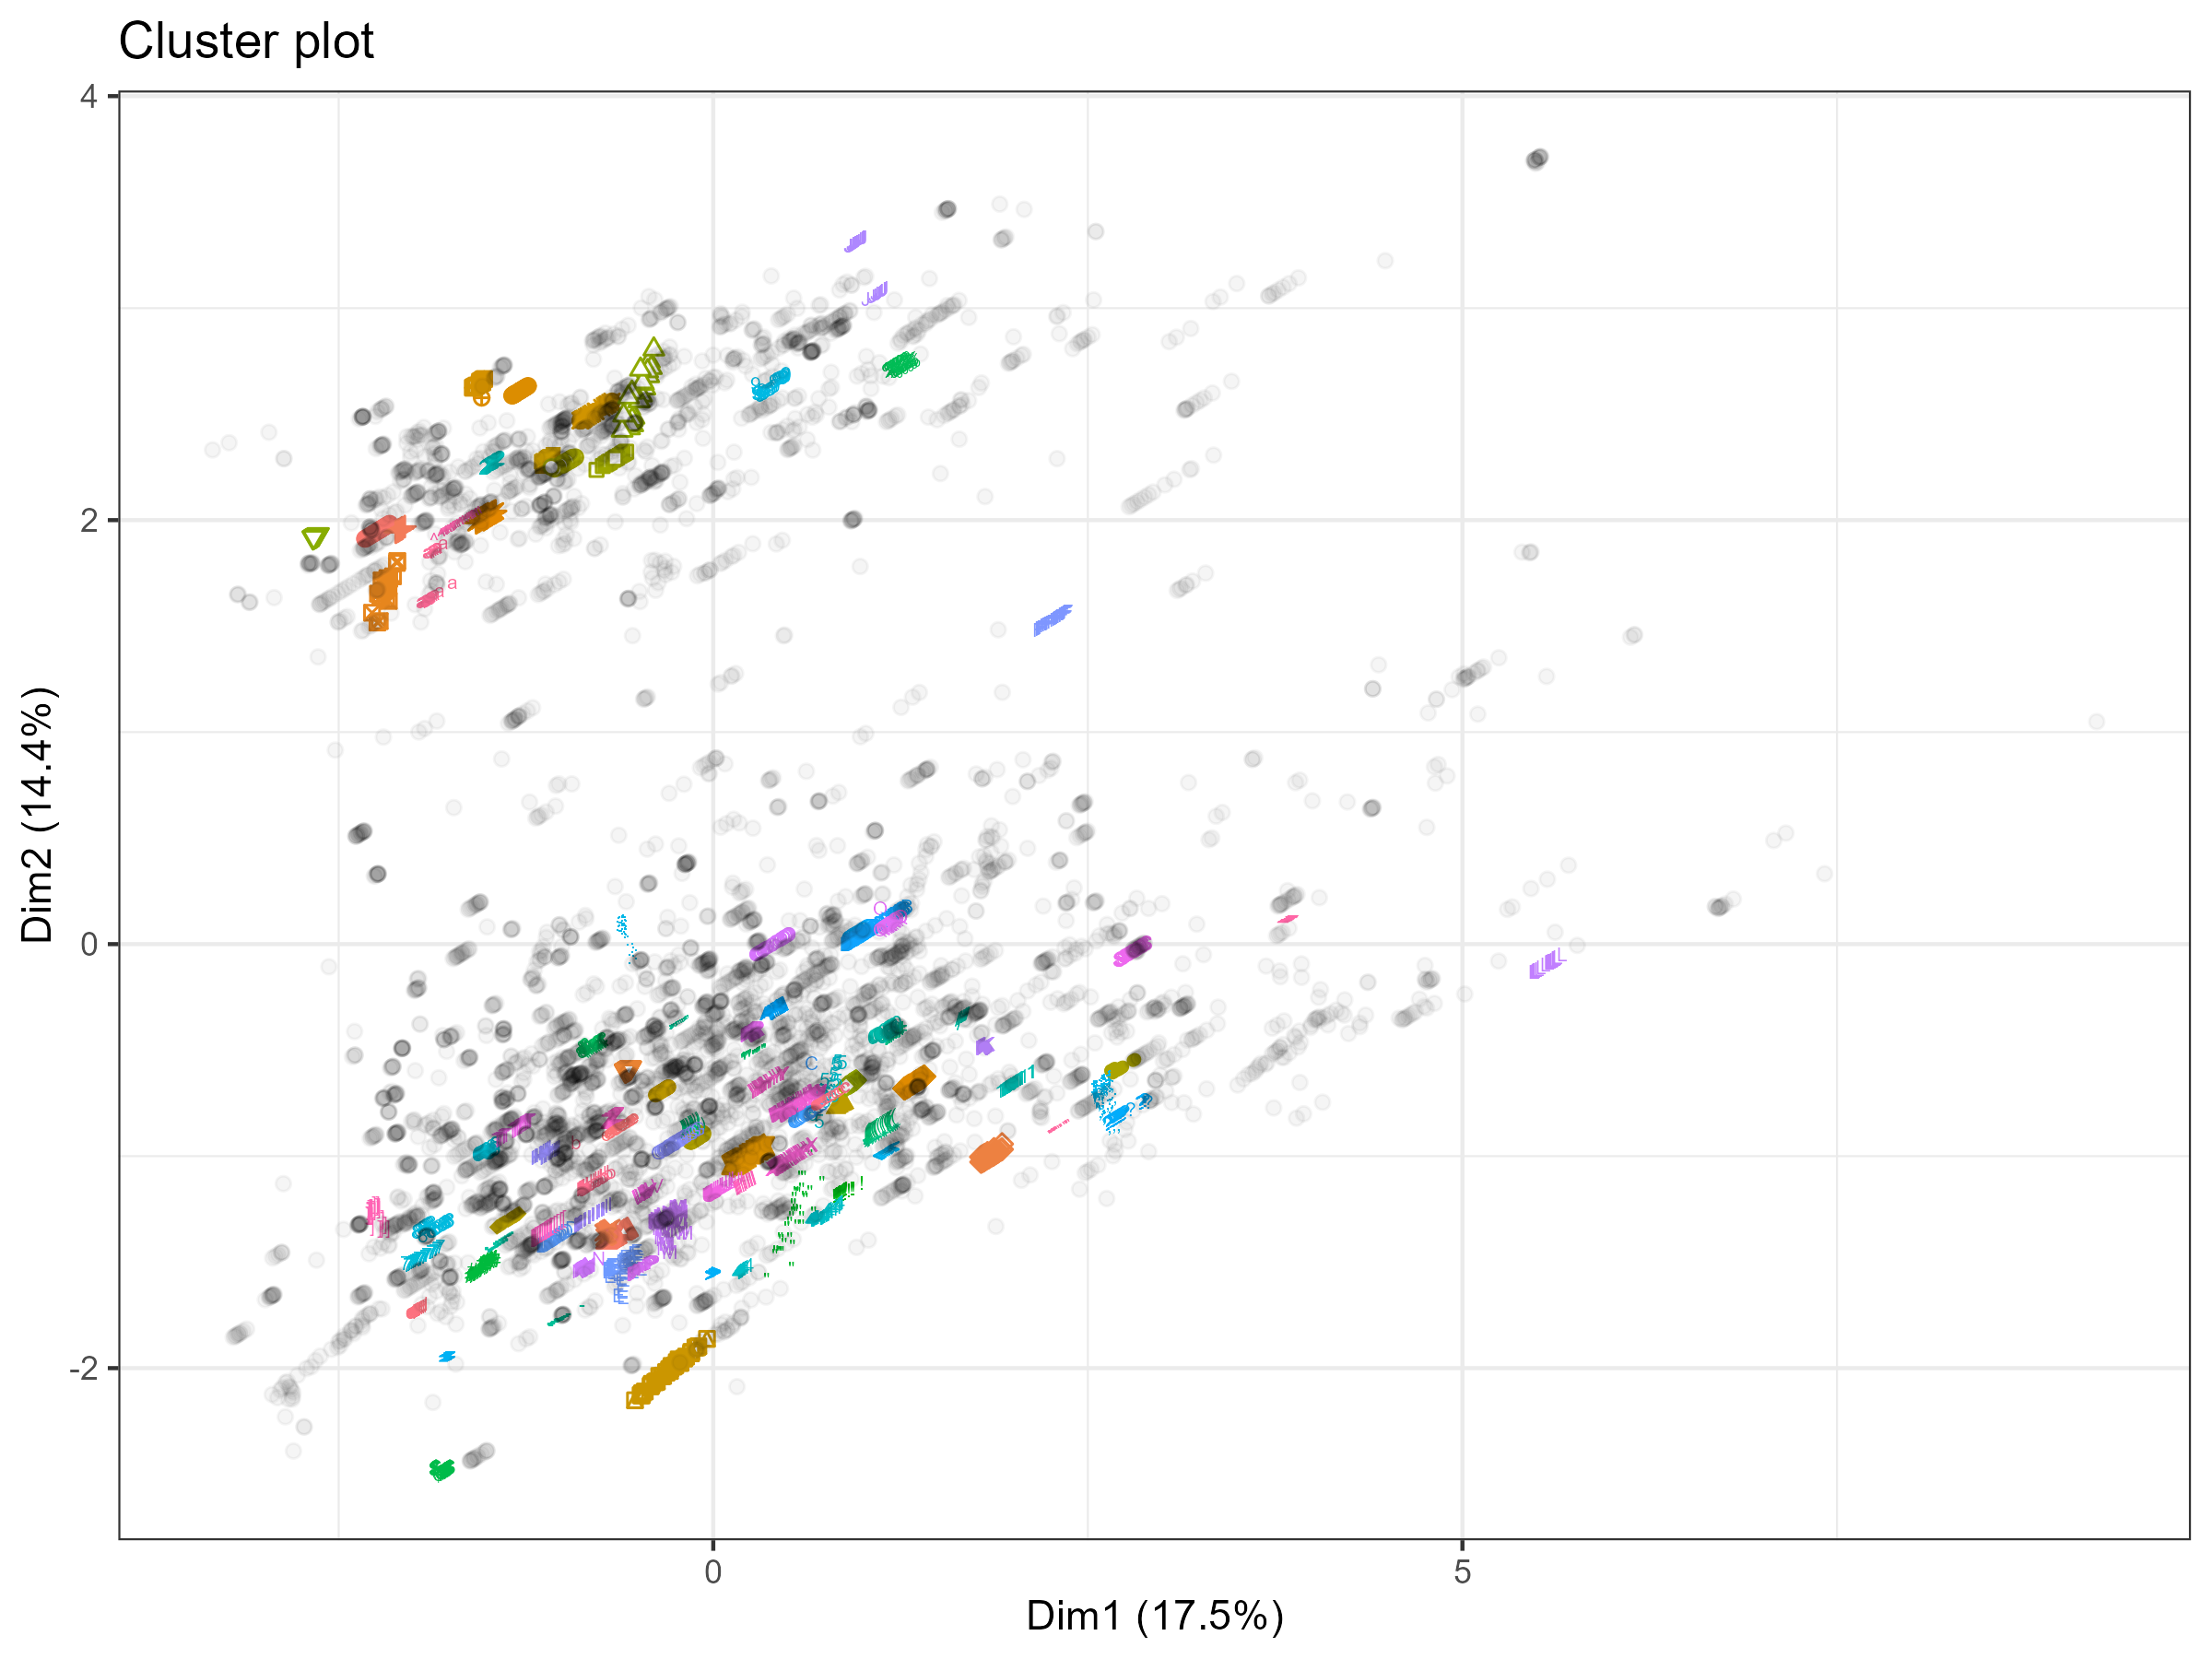
\includegraphics[width=0.8\textwidth]{Images/4_clustering/DBSCAN/baddbscan.png}
    \caption{Resultats del clústering inicial usant DBSCAN (0.15, 20) visualitzats en els dos primers components principals \\
    Des d'aquest punt tots els clústerings seran visualitzats d'aquesta manera.}
    \label{fig:DBSCAN_inicial}
\end{figure}


Per millorar els resultats, calia trobar la millor epsilon i el millor mínim de punts. Pel mínim de punts, es va escollir el 0.25\%, en aquest cas 22 punts. És un valor gran, però cal tenir en compte que la nostra base de dades també és bastant gran, amb 8800 observacions. Per escollir la epsilon, s'han realitzat les distàncies de knn, i s'ha intentat escollir el que tenia canvi de pendent màxim. Aquest retornava una epsilon de 0.72, però analitzant el gràfic s'ha determinat que un millor valor era 0.55. Tornant a realitzar el DBSCAN obteniem la figura  (figura \ref{fig:DBSCAN_auto}):

\begin{figure}[H]
    \centering
    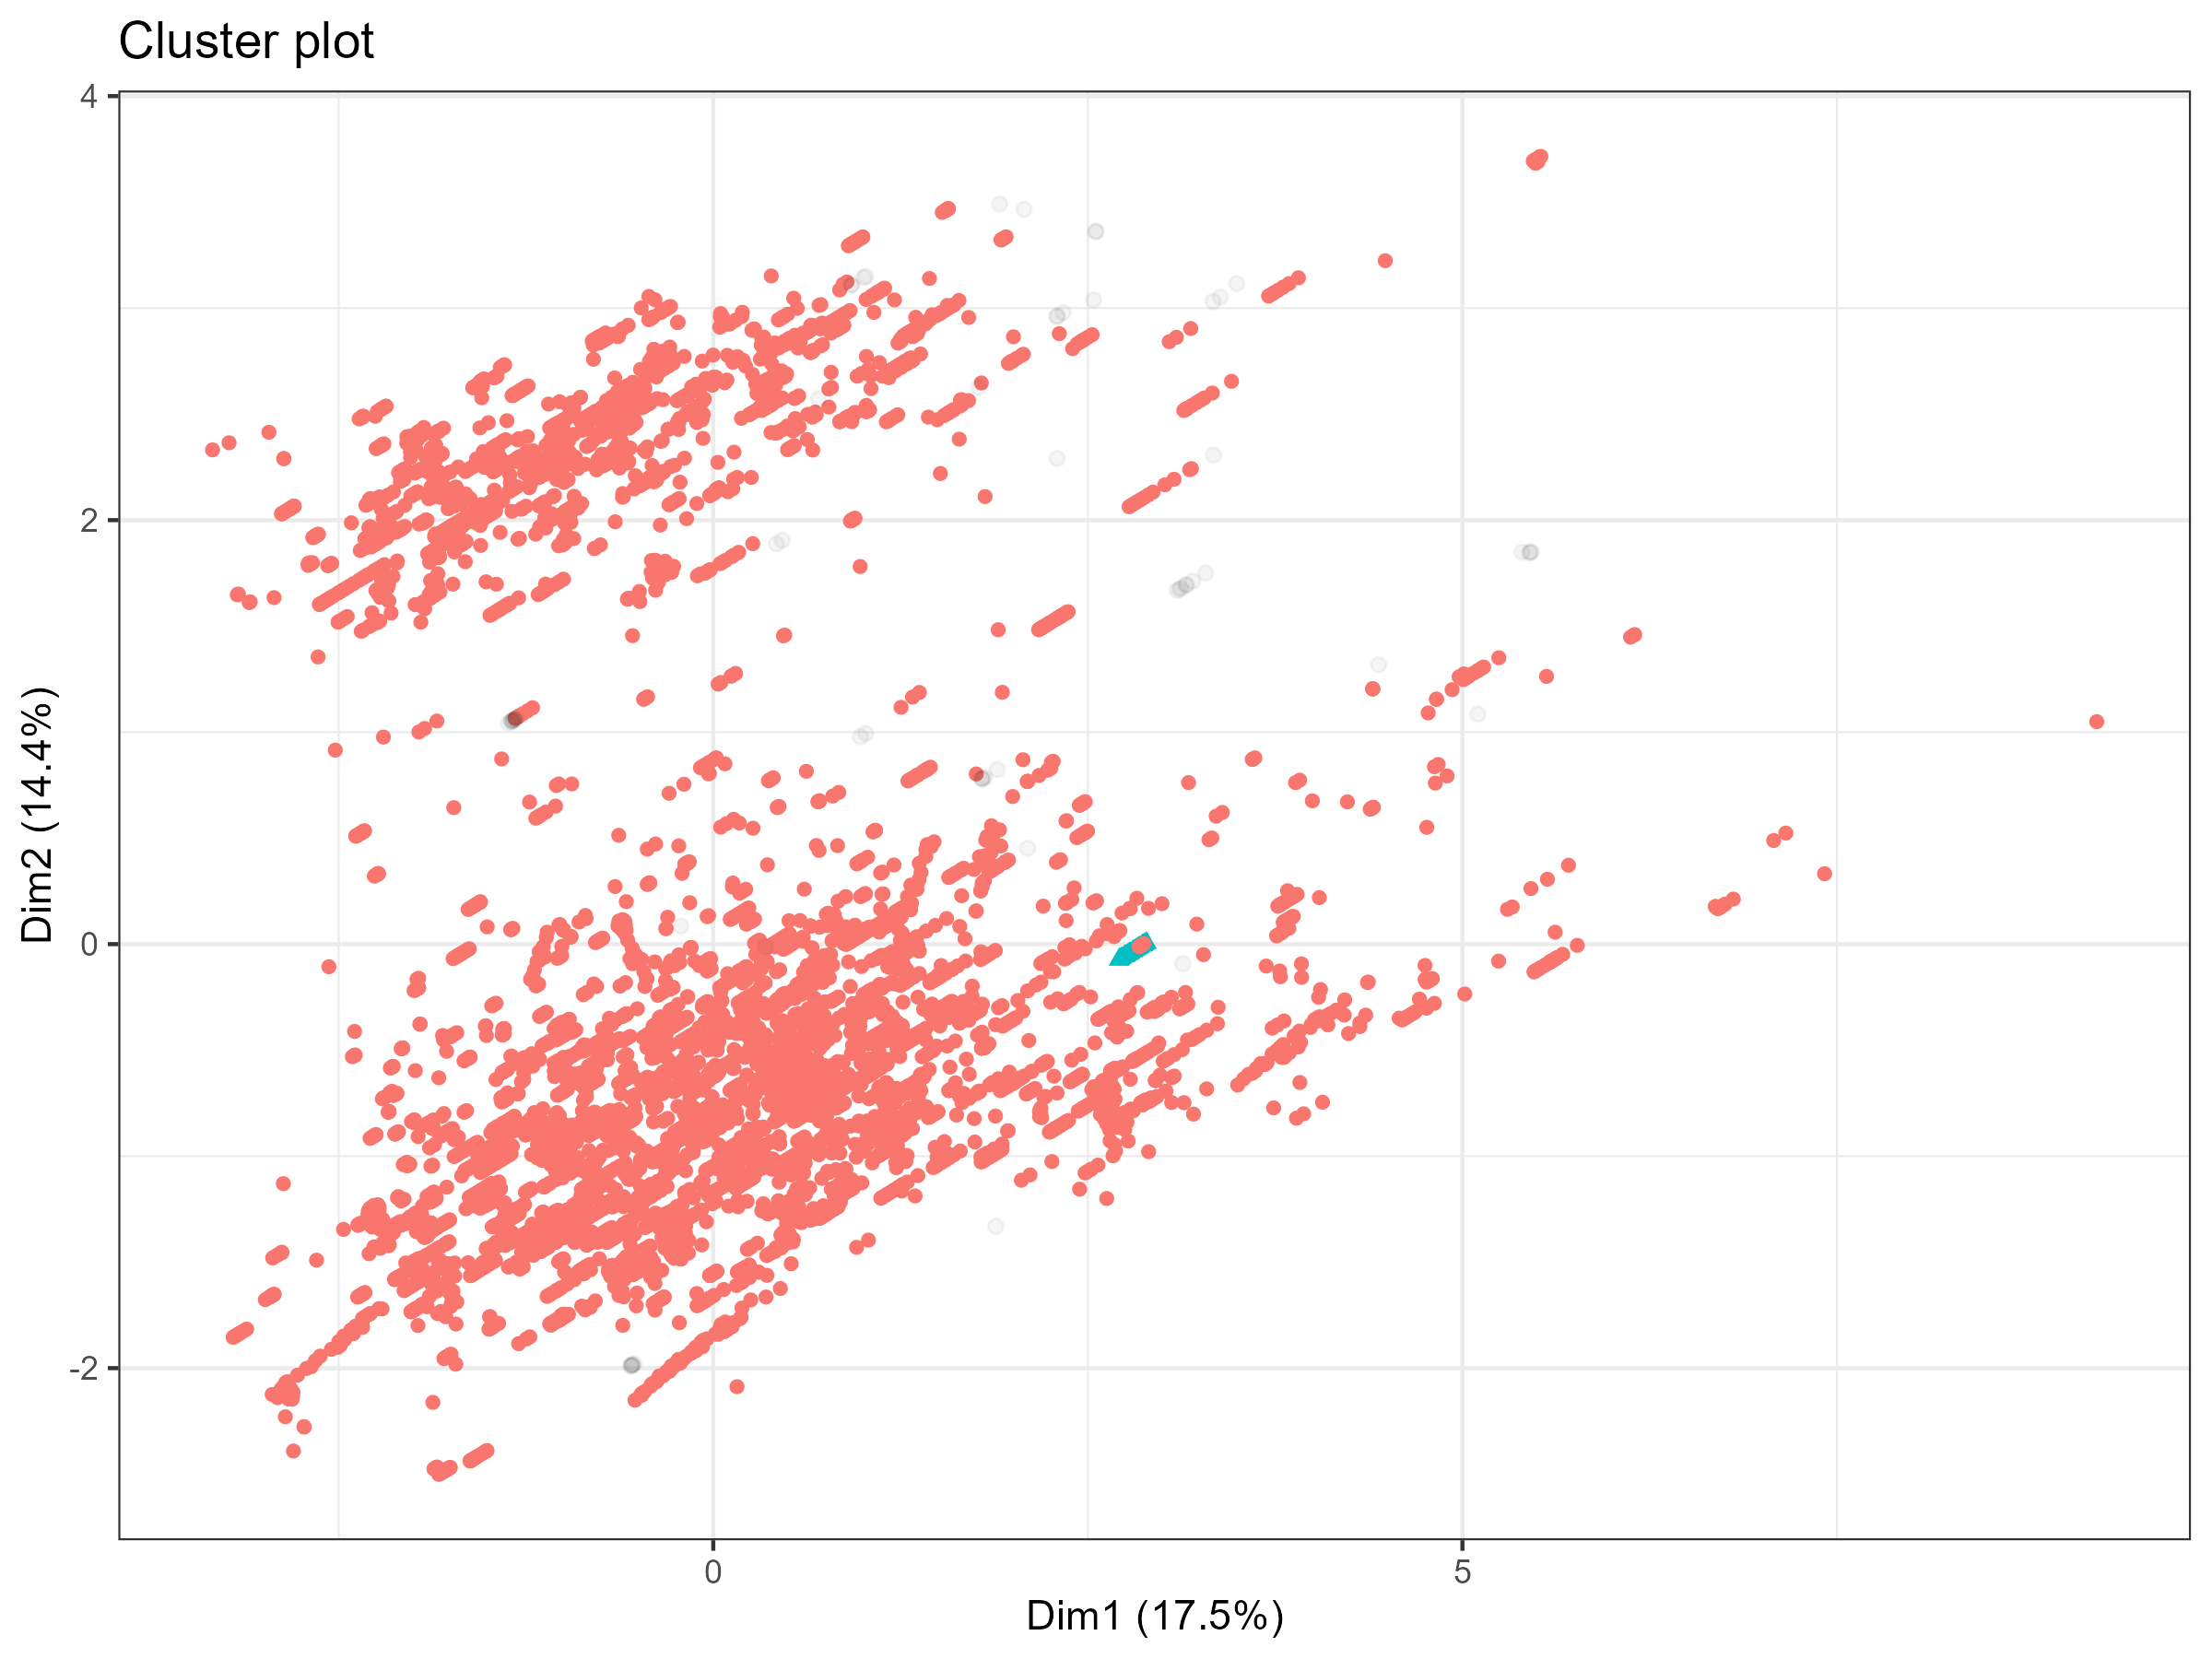
\includegraphics[width=0.8\textwidth]{Images/4_clustering/DBSCAN/dbscanauto.png}
    \caption{Resultats del clústering usant DBSCAN, epsilon knn (0.55, 22)}
    \label{fig:DBSCAN_auto}
\end{figure}

Es pot veure com aquests valors no han servit gens per millorar els resultats: ara, enlloc d'haver-hi molts clústers petits, n'hi ha un de molt gran. En teoria n'hi ha dos més, però son tan petits que són pràcticament imperceptibles.

Buscant de forma artificial uns valors de èpsilon i de mínim de punts, el resultat del DBSCAN ha sigut millor (figura \ref{fig:DBSCAN_manual}), tot i que no ha variat gaire respecte al k means: hem trobat els dos grans grups esmentats anteriorment. Per fer-ho, s'ha usat una epsilon de 0.4 i un mínim de punts de 70 (molt elevat). Amb valors més petits de mínim de punts, apareixien altre cop els clústers molt petits, que no aporten gaire res. Jugant amb la epsilon (per exemple, 0.35) es van obtenir alguns clústers dins del clúster gran de baix: un amb els valors més baixos de la dimensió 2, un altre amb els valors més alts de la dimensió 1 i un altre amb valors alts de les dues dimensions (figura \ref{fig:DBSCAN_manual2}). Tot i això, aquests clústers eren bastant petits.

\begin{figure}[H]
    \centering
    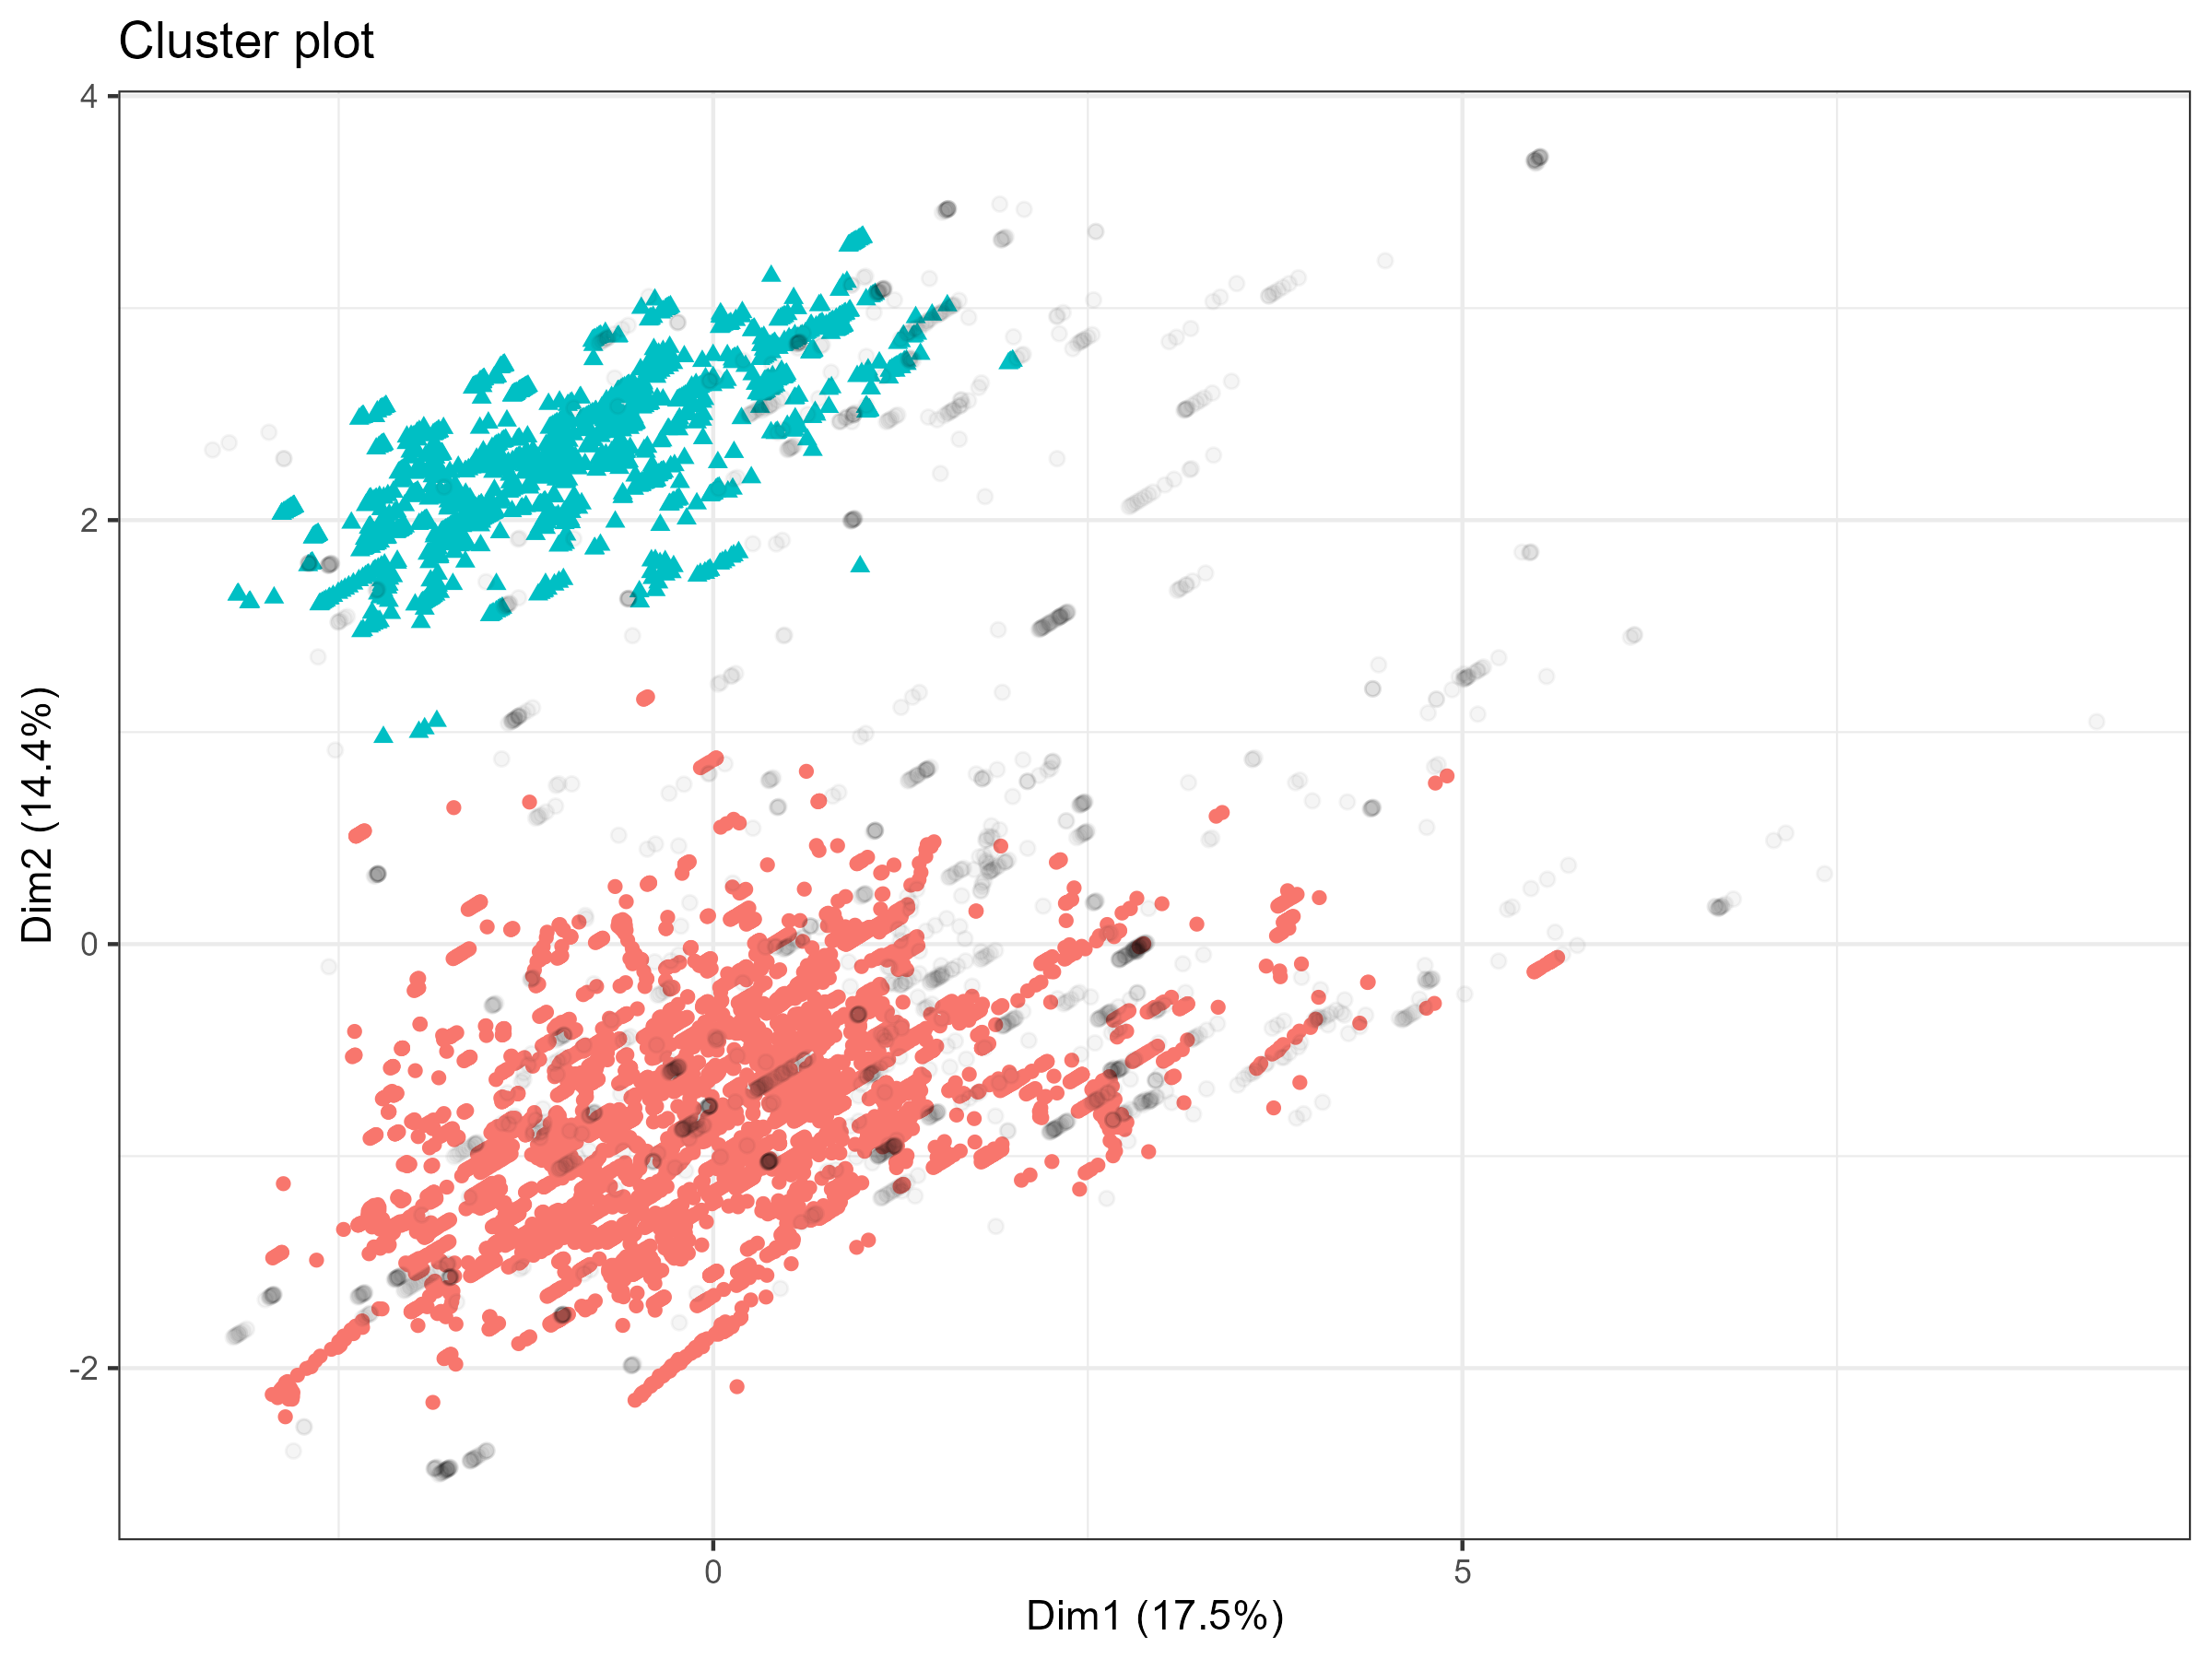
\includegraphics[width=0.8\textwidth]{Images/4_clustering/DBSCAN/dbscanforca.png}
    \caption{Resultats del clústering usant DBSCAN, epsilon manual (0.4, 70)}
    \label{fig:DBSCAN_manual}
\end{figure}

\begin{figure}[H]
    \centering
    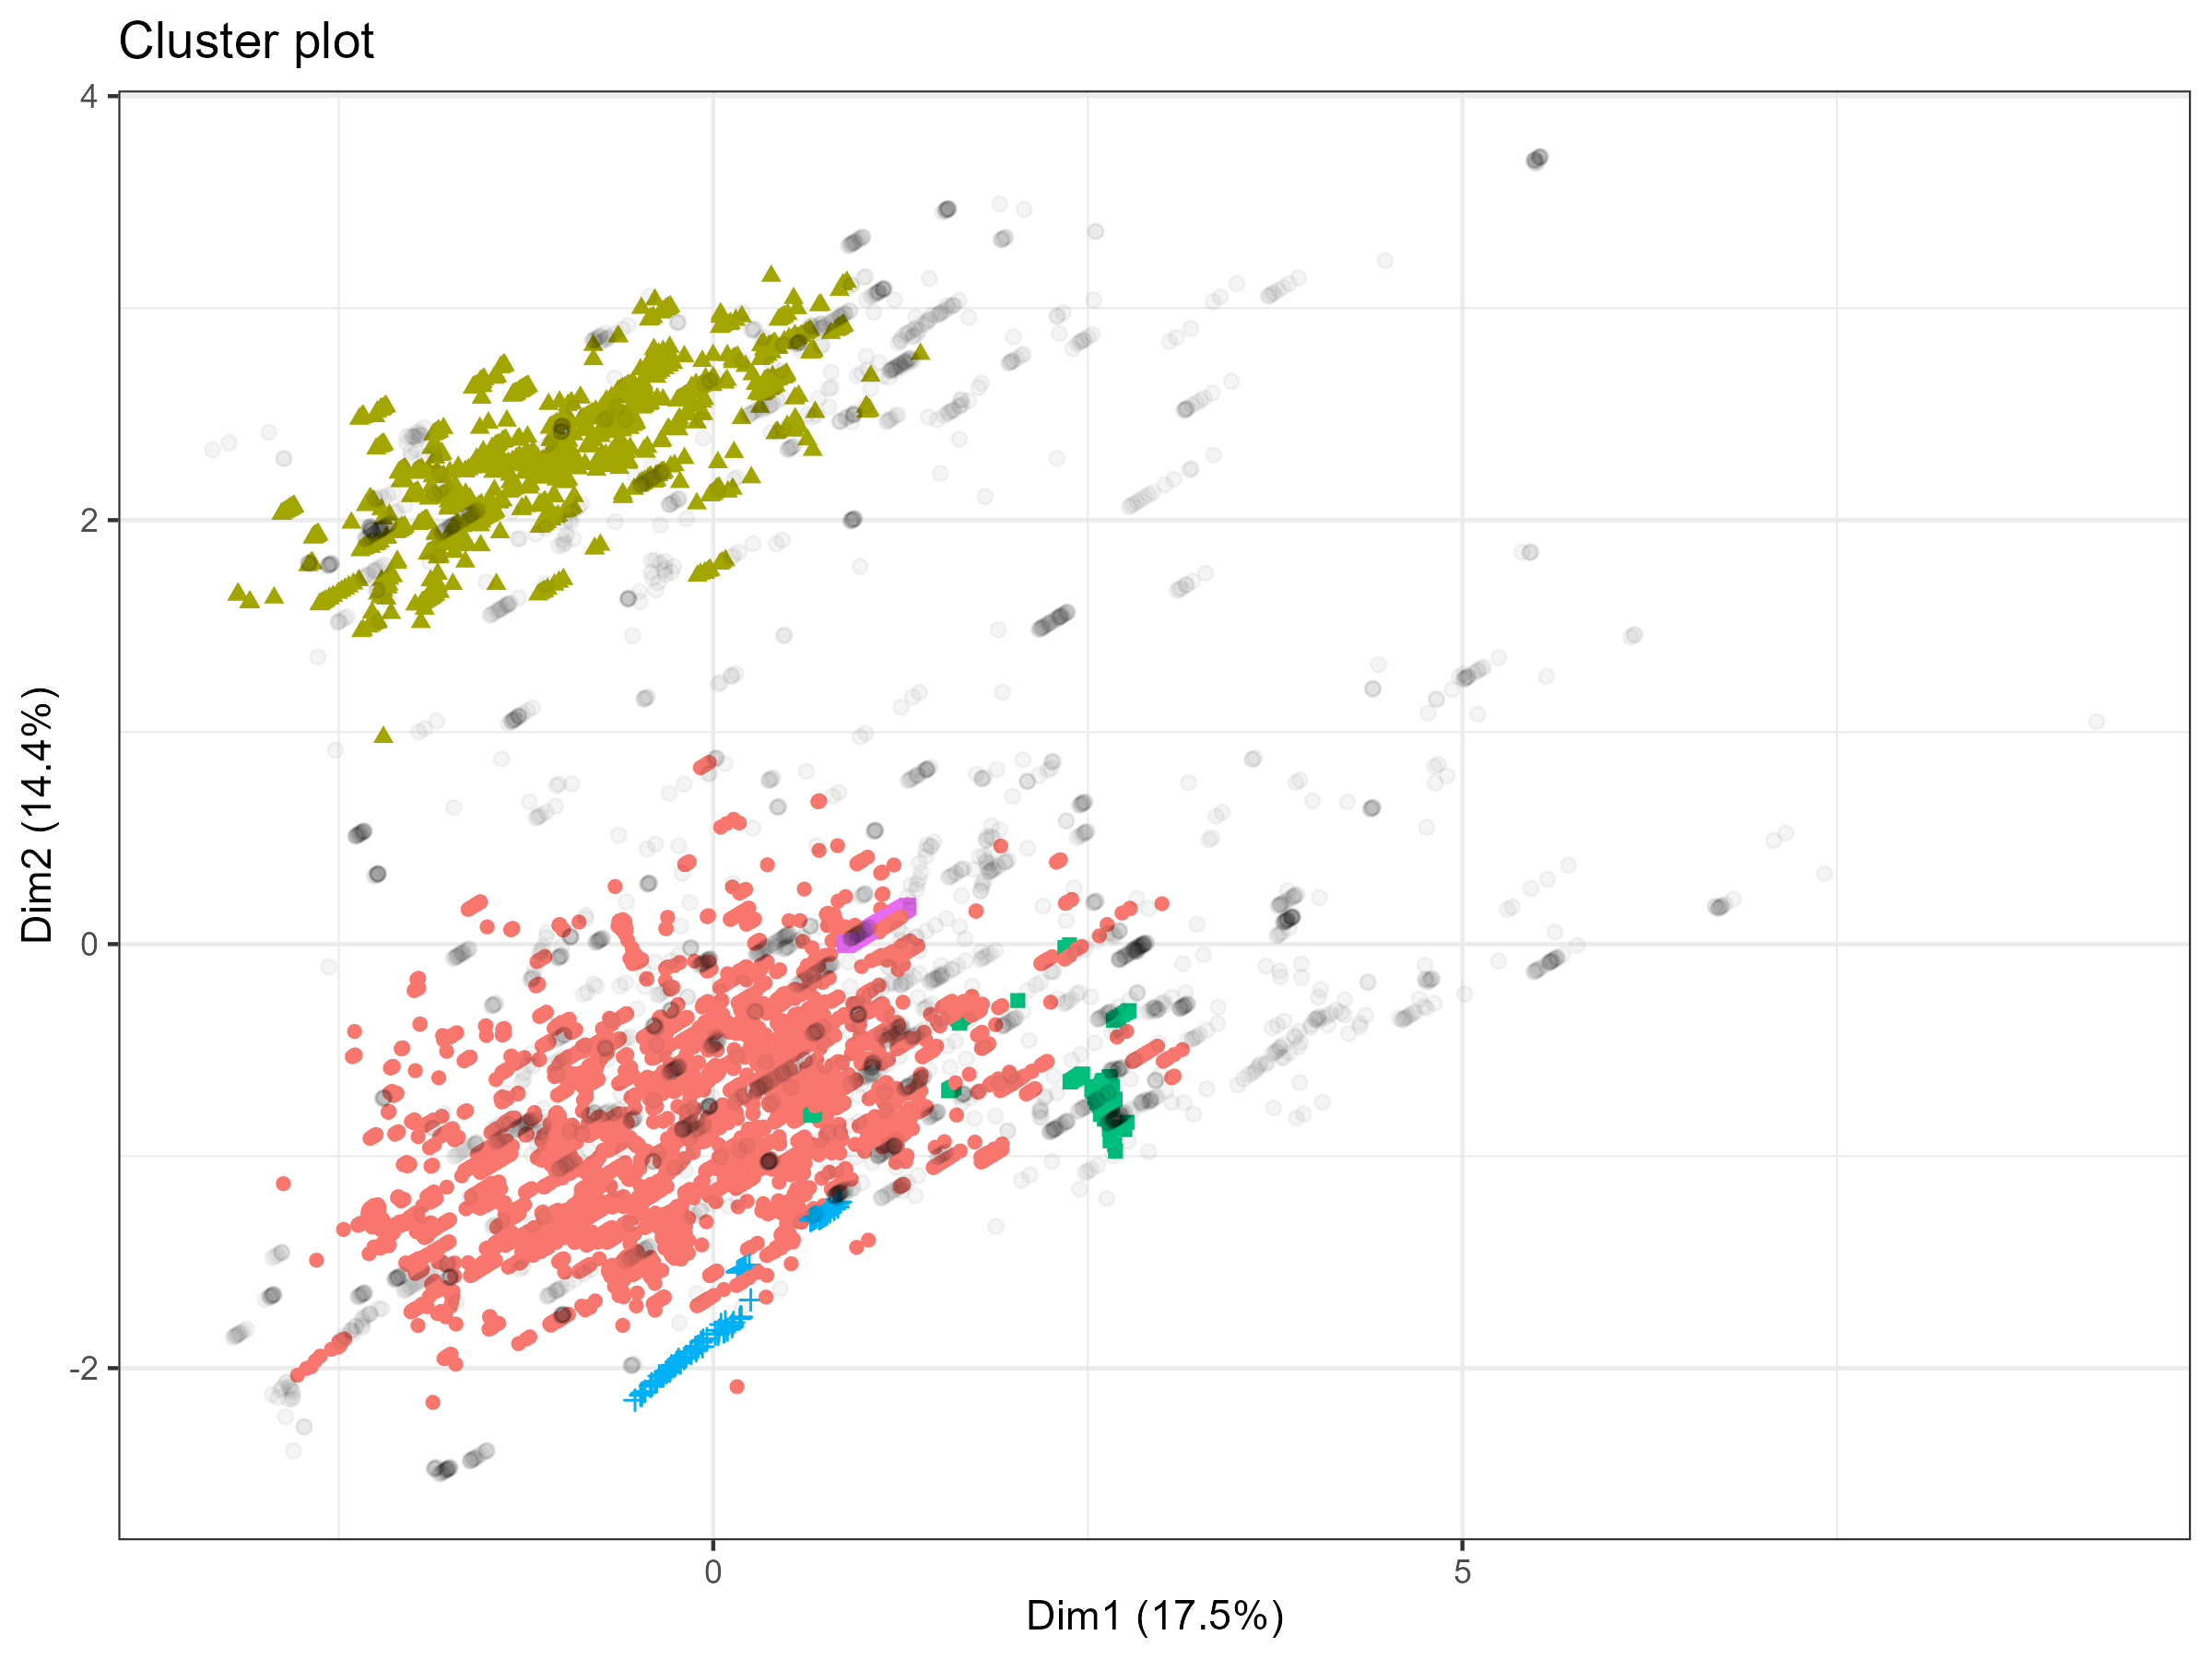
\includegraphics[width=0.8\textwidth]{Images/4_clustering/DBSCAN/dbscanforcaalt.png}
    \caption{Resultats del clústering usant DBSCAN, epsilon manual v2 (0.35, 70)}
    \label{fig:DBSCAN_manual2}
\end{figure}

En aquest apartat, el clústering escollit després de valorar totes les opcions ha sigut el DBSCAN usant epsilon 0.47 i minPts 70. Amb aquest obtenim les dues classes que s'han comentat, i 508 outliers.

A més del DBSCAN, es plantejava usar un algorisme derivat d’aquest, però que usa una tècnica diferent: OPTICS (\cite{ankerst_1999_optics}). Aquest analitza on “pot anar” cada punt, assignant-li una \textit{reachability}. En la base de dades, el reachability plot, usant els paràmetres epsilon 0.55 i minPts 22 es poden observar a la figura \ref{fig:OPTICS_inicial}.

\begin{figure}[H]
    \centering
    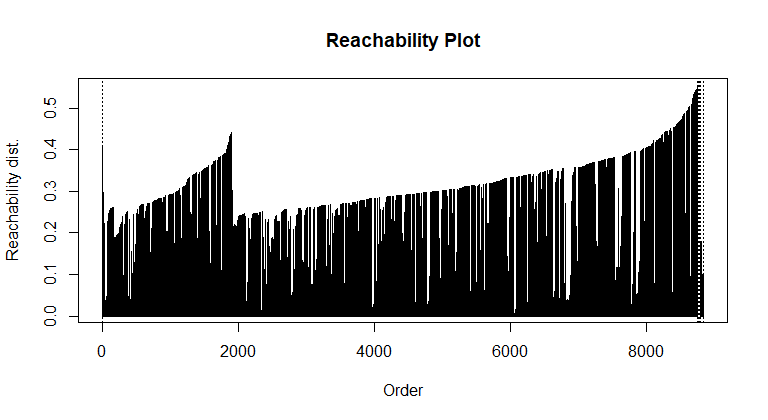
\includegraphics[width=0.8\textwidth]{Images/4_clustering/optics/reachability1.png}
    \caption{Reachability de OPTICS inicial (0.55, 22)}
    \label{fig:OPTICS_inicial}
\end{figure}

Per tal d'escollir un altre epsilon i minPts que anés millor, s'ha provat utilitzant un Grid Search tots els epsilon entre 0.1 i 1 de 0.05 en 0.05 i tots els minPts entre 10 i 70 de 10 en 10. Després d'aquesta cera, els millors valors escollits han estat 0.9 i 10 punts. El Reachability plot queda, tallant a 0.4, tal que (figura \ref{fig:OPTICS_grid}):

\begin{figure}[H]
    \centering
    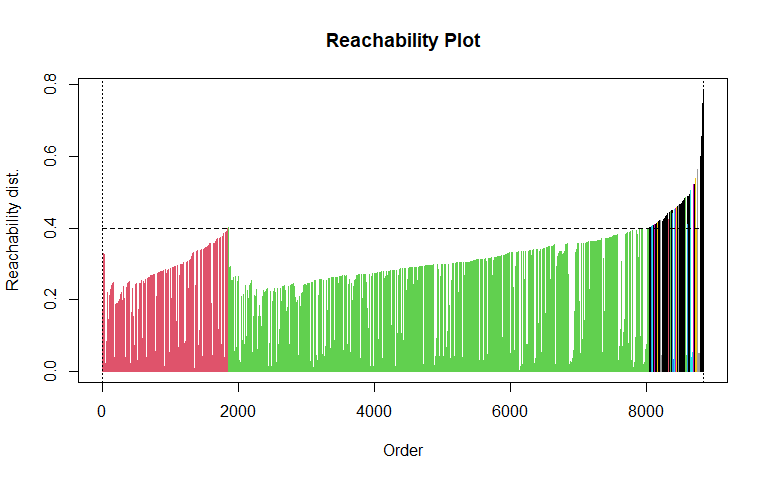
\includegraphics[width=0.8\textwidth]{Images/4_clustering/optics/reachabilitygrid.png}
    \caption{Reachability de OPTICS usant grid search (0.9, 10)}
    \label{fig:OPTICS_grid}
\end{figure}

D'aquí, podem extreure un clústering que es pot visualitzar igual que feiem amb el DBSCAN (figura \ref{fig:OPTICS_grid_res}).

\begin{figure}[H]
    \centering
    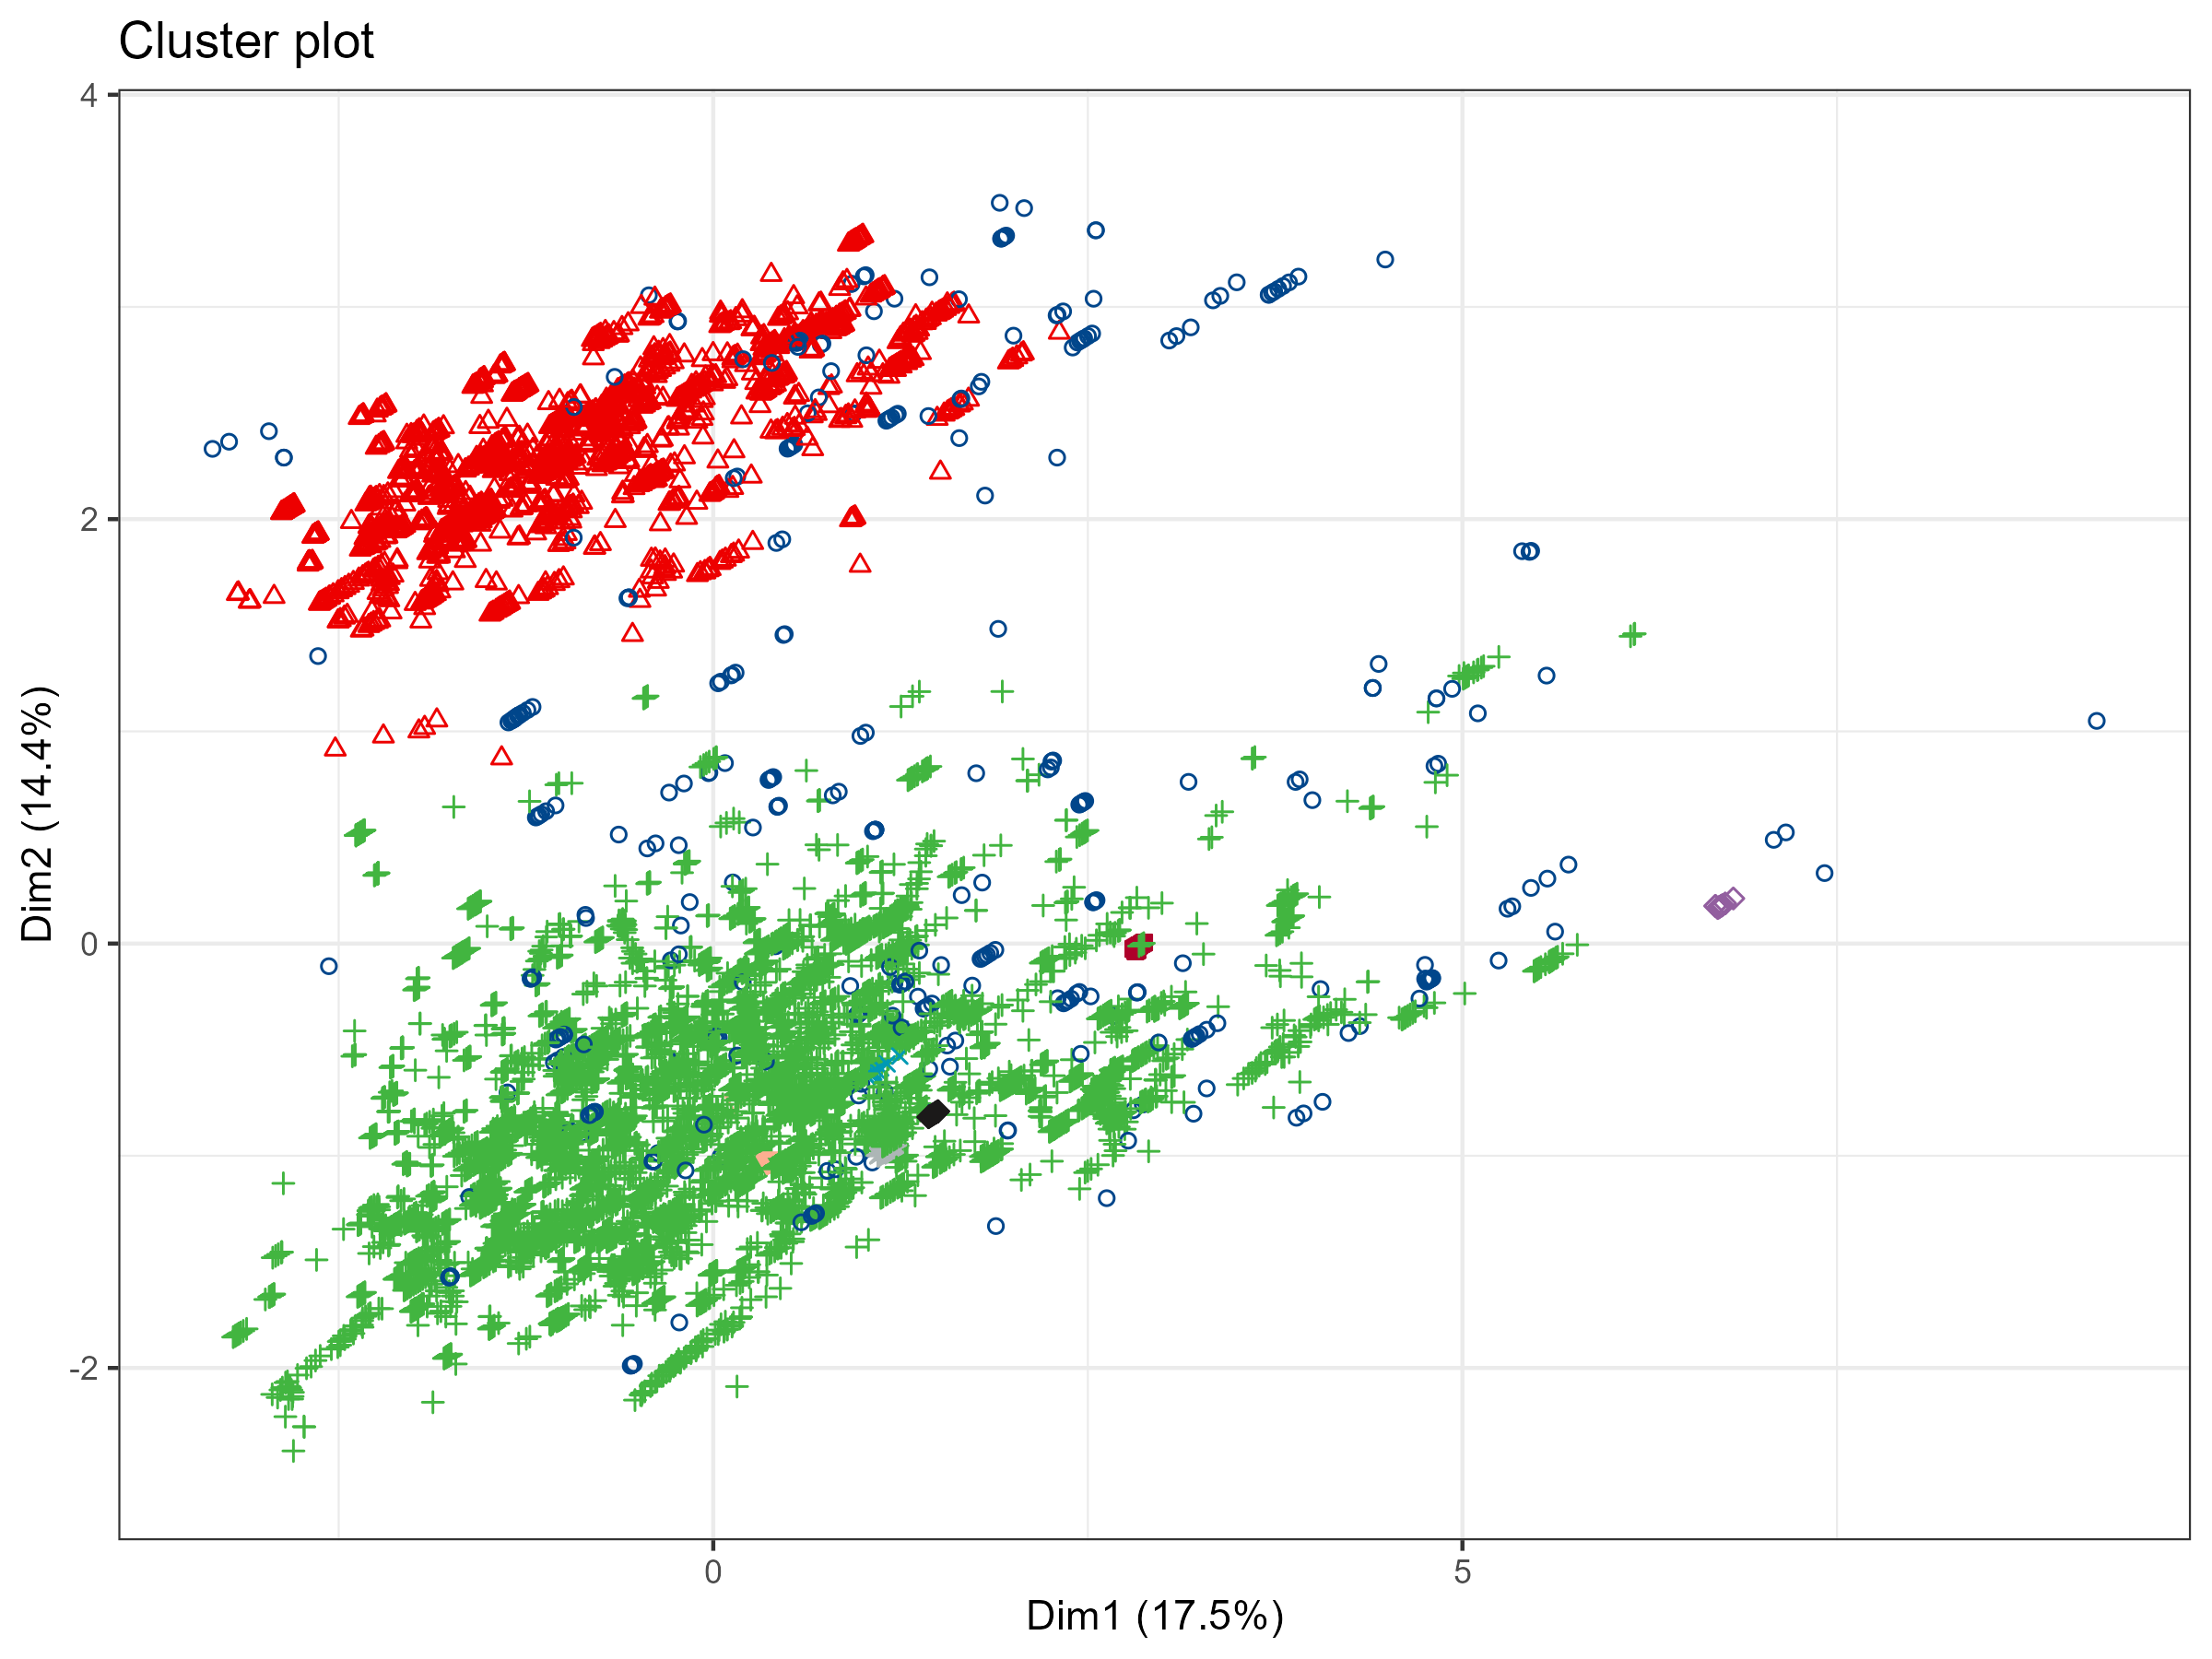
\includegraphics[width=0.8\textwidth]{Images/4_clustering/optics/opticsgrid.png}
    \caption{Resultats del clústering usant OPTICS, grid search (0.9, 10)}
    \label{fig:OPTICS_grid_res}
\end{figure}


S'observen dos clústers principals (tot i que realment n'hi ha uns 20). També veiem bastants outliers (en total 792) i clústers petits al sector dret, similar als que veiem amb el DBSCAN. L'alternativa a aquest gridSearch era usar el silhouette, però no dóna bons resultats en aquest cas, creant més de 300 clústers diferents (figura \ref{fig:OPTICS_silo}).
\begin{figure}[H]
    \centering
    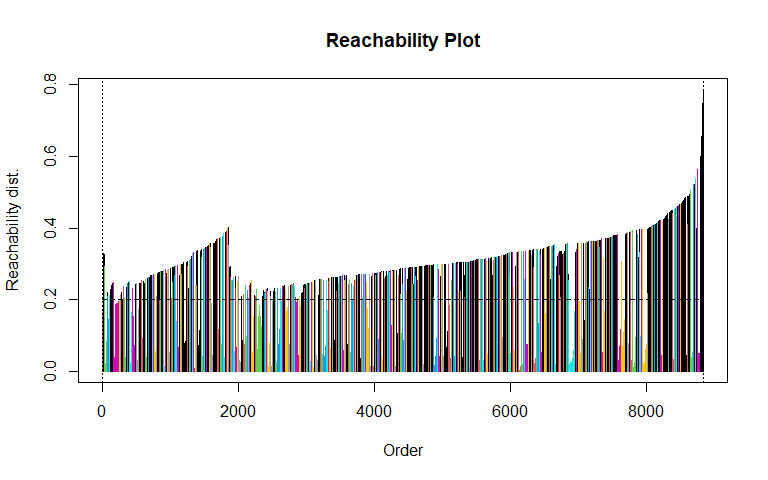
\includegraphics[width=0.8\textwidth]{Images/4_clustering/optics/siloreachability.png}
    \caption{Reachability de OPTICS usant silhouette (0.2, 22)}
    \label{fig:OPTICS_silo}
\end{figure}

En conclusió, sembla ser que l'optics no és una bona tècnica de clústering per aquestes dades. Com a molt, és capaç d'acostar-se als resultats obtinguts amb el DBSCAN. En general, les dues tècniques no han sigut capaces de crear clústers lo suficientment interessants i equilibrats com per poder extreure'n bona informació, o sigui que probablement no siguin les millors per aquestes dades. En aquest cas, el KMEANS creava uns clústers més interessants, i encara que no detectés outliers, probablement serien agrupacions més interessants.


\subsection{Clústering de sèries temporals}

S'ha realitzat una anàlisi de clústering de sèries temporals per a les cançons més escoltades mensualment a Spotify entre els anys 2017 i 2021. L'objectiu ha estat identificar patrons de comportament en les tendències de streams, que poden revelar agrupacions de cançons amb trajectòries similars en el temps, incloent hits ràpids o cançons amb una presència sostinguda en el temps.

Per dur a terme aquesta anàlisi, primer s'han carregat i preparat les dades, transformant-les per adequar-se a l'anàlisi de sèries temporals. Aquesta preparació ha inclòs la transformació de les variables \texttt{year\_week} i \texttt{month\_week} en una única columna de text per al mes i any, així com la pivotació de les dades per tenir aquesta nova variable \texttt{year\_month} en columnes i \texttt{track\_name} en files. Per a cada valor de fila i columna es va fer una agregació de totes les reproduccions de la cançó en aquell mes en concret.

S'ha seleccionat la variable \texttt{streams} per a l'anàlisi, considerant que aquesta proporcionaria el major benefici per a l'empresa al analitzar les cançons amb tendències de popularitat ràpida o sostinguda. S'ha prestat molta atenció al fet que, degut a que les dades només inclouen les cançons que estan dins del top 40 global de Spotify, les streams d'una cançó en un mes on no apareix cap vegada s'han considerat com a 0. Aquesta aproximació s'ha justificat amb l'ús de la Distància Temporal Dinàmica (DTW) per al càlcul de similituds, entenent que els valors 0 tenen menys pes en la comparació, i per tant, l'anàlisi es centra més en les tendències presents que en les absències.

Amb les dades preparades, s'ha realitzat un clústering jeràrquic utilitzant la distància DTW i el mètode de Ward. Aquest mètode s'ha escollit per la seva capacitat de crear grups basats en la minimització de la variància dins dels clústers, ideal per identificar grups de cançons amb patrons de streams similars al llarg del temps. 

Després de l'anàlisi jeràrquic, s'ha realitzat el dendrograma per poder escollir quin és el nombre més adequat de classes.

\begin{figure}[H]
    \centering
    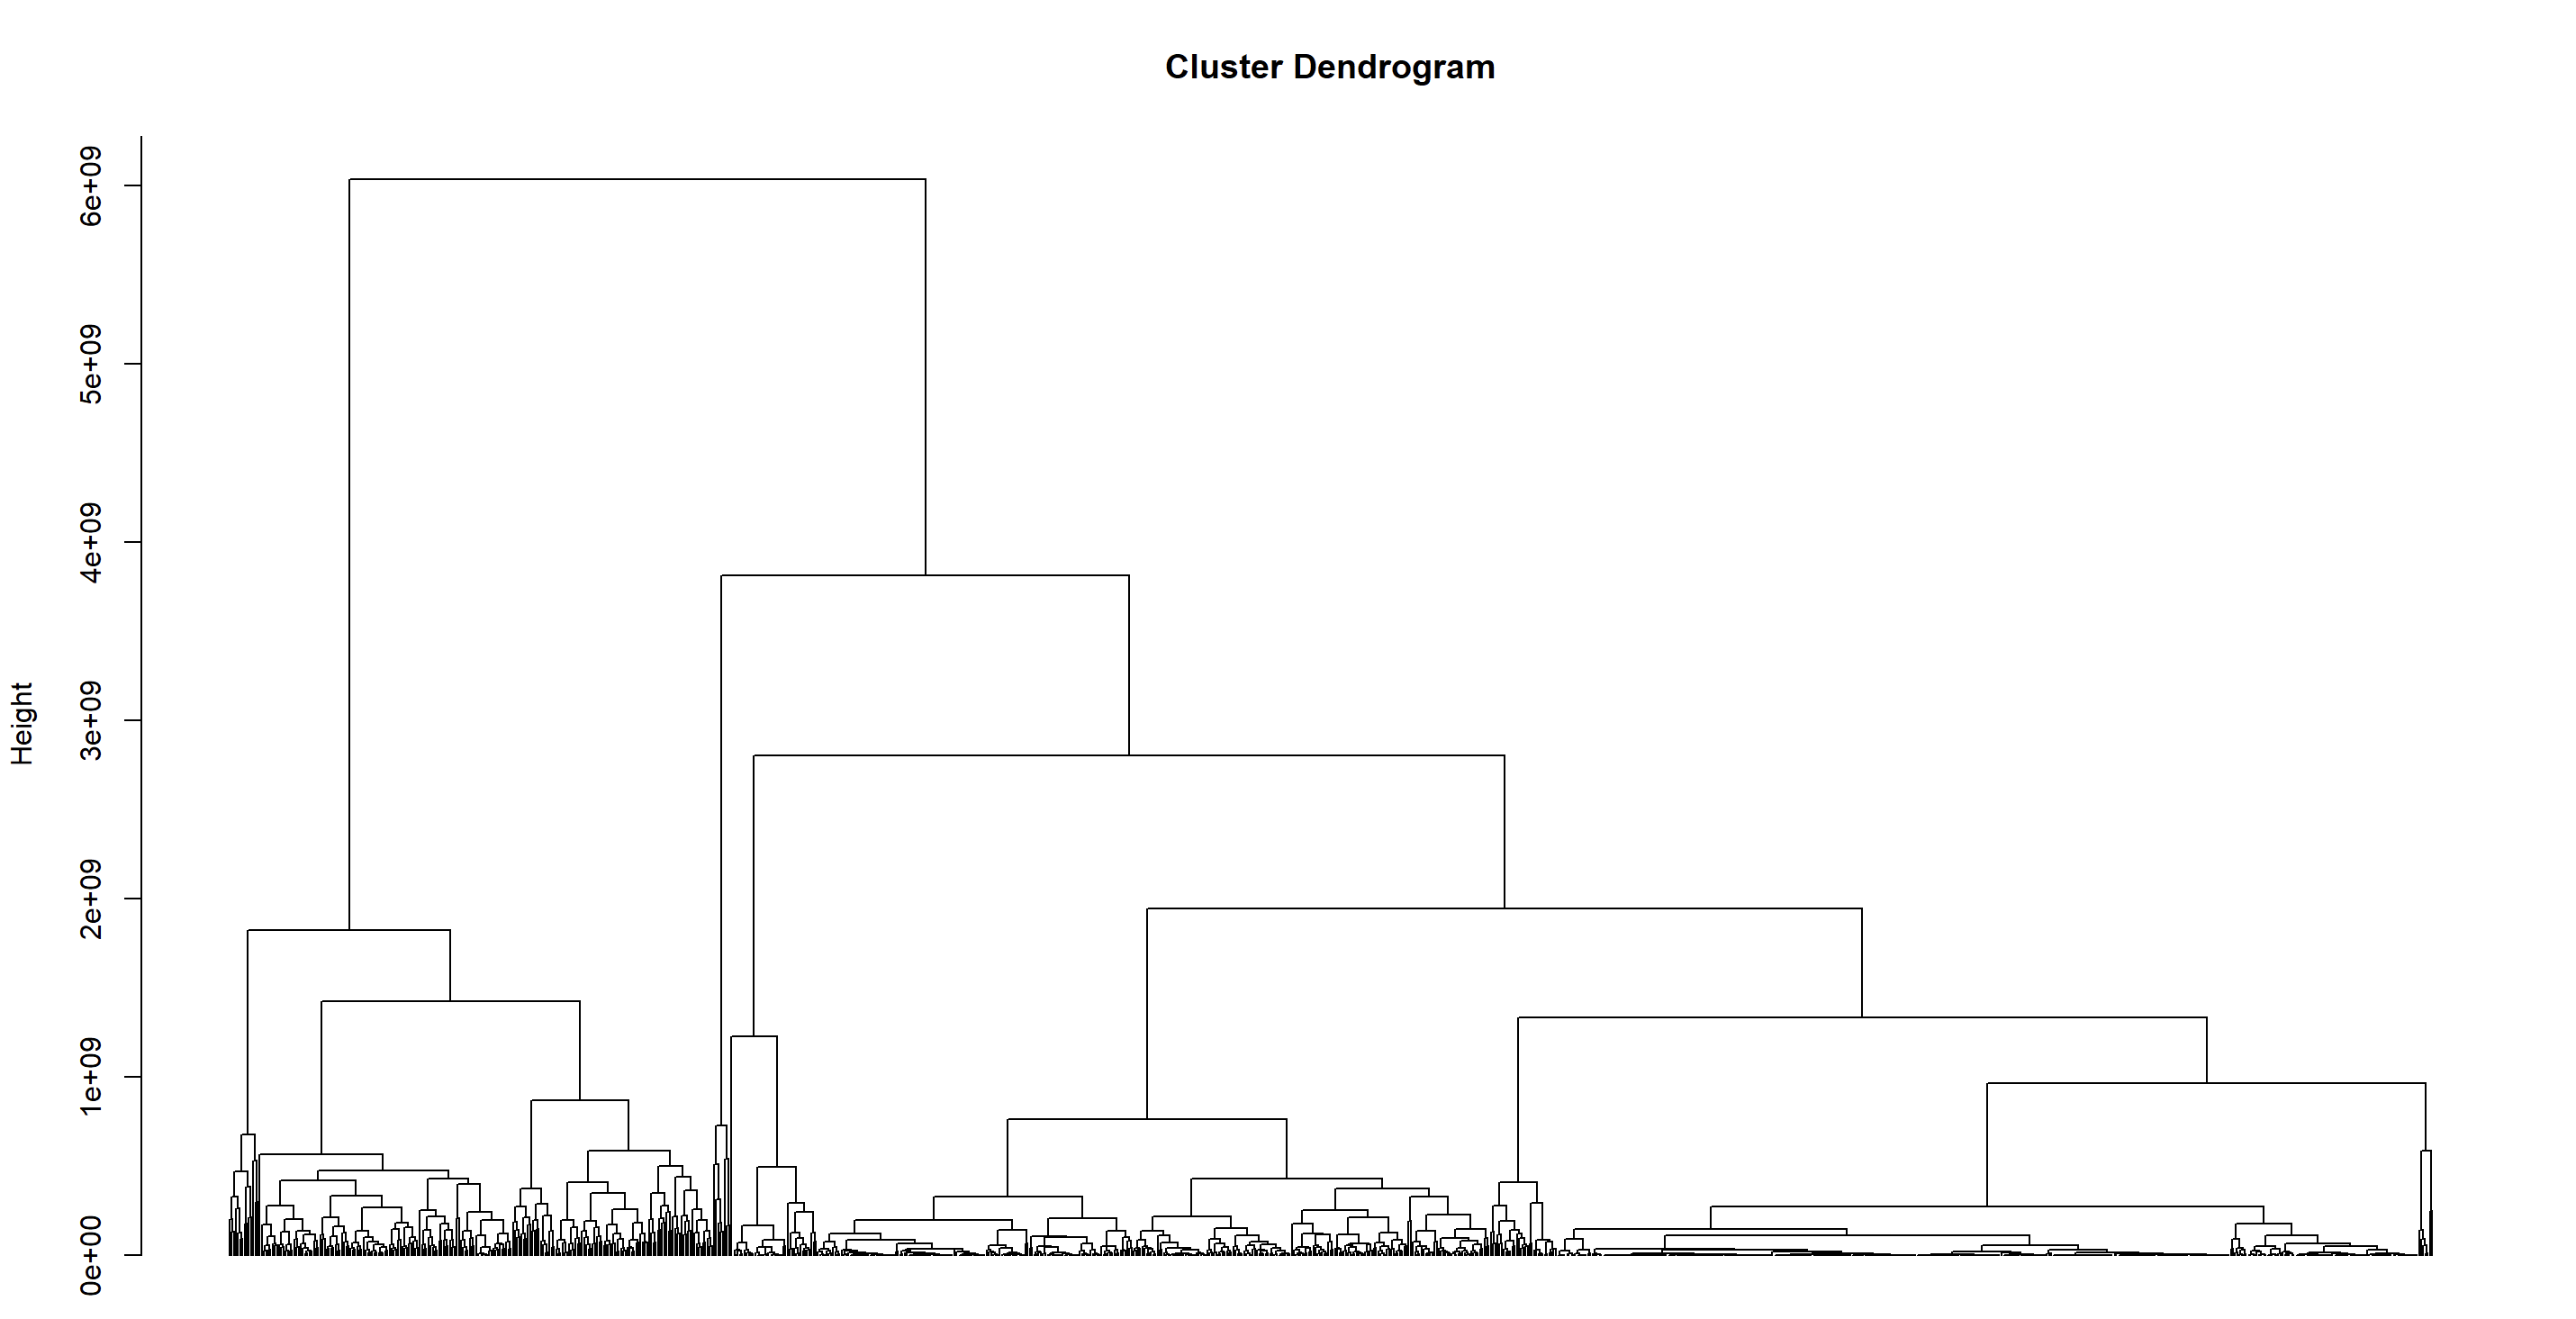
\includegraphics[width=\textwidth]{Images/4_clustering/time_series/dendrograma_original.png}
    \caption{Dendrograma de cançons utilitzant distància \texttt{DTW} i mètode \texttt{ward.D2}}
    \label{fig:TS_dendrograma_original}
\end{figure}

Com es pot veure en la figura \ref{fig:TS_dendrograma_original} el nombre \textit{k} a escollir no és gaire evident degut al desbalanceig de la majoria de clústers. Després d'analitzar aquest equilibri de classes, s'ha realitzat un tall per obtenir 5 classes diferents per tal d'intentar tenir una quantitat de cançons similar a tots els clústers (intentant mantenir una \textit{k} petita igualment).

Com es pot veure en la següent taula \ref{tab:TS_clustering_results} les 3 primeres classes tenen un nombre prou equilibrat de cançons mentre que en el quart n'hi ha moltes menys i en el cinquè gairebé no n'hi ha cap. Aquest fet és curiós degut a que molt probablement aquestes cançons agrupades en classes tan reduïdes podrien estar molt relacionades entre si podent arribar a conclusions interessants.

\begin{table}[H]
\centering
\begin{tabular}{|c|c|c|c|c|}
\hline
1    & 2    & 3   & 4   & 5 \\ \hline
311 & 436 & 224 & 40 & 8  \\ \hline
\end{tabular}
\caption{Resultat del clústering de les sèries temporals}
\label{tab:TS_clustering_results}
\end{table}

Una vegada s'ha escollit el valor de $k = 5$, en la figura \ref{fig:TS_dendrograma_colors} es pot veure el dendrograma colorejat per tal de visualitzar els diferents clústers. El color verd representa el clúster número 3, el color lila el 5, el blau el 4, el vermell l'1 i el mostassa el 2.

\begin{figure}[H]
    \centering
    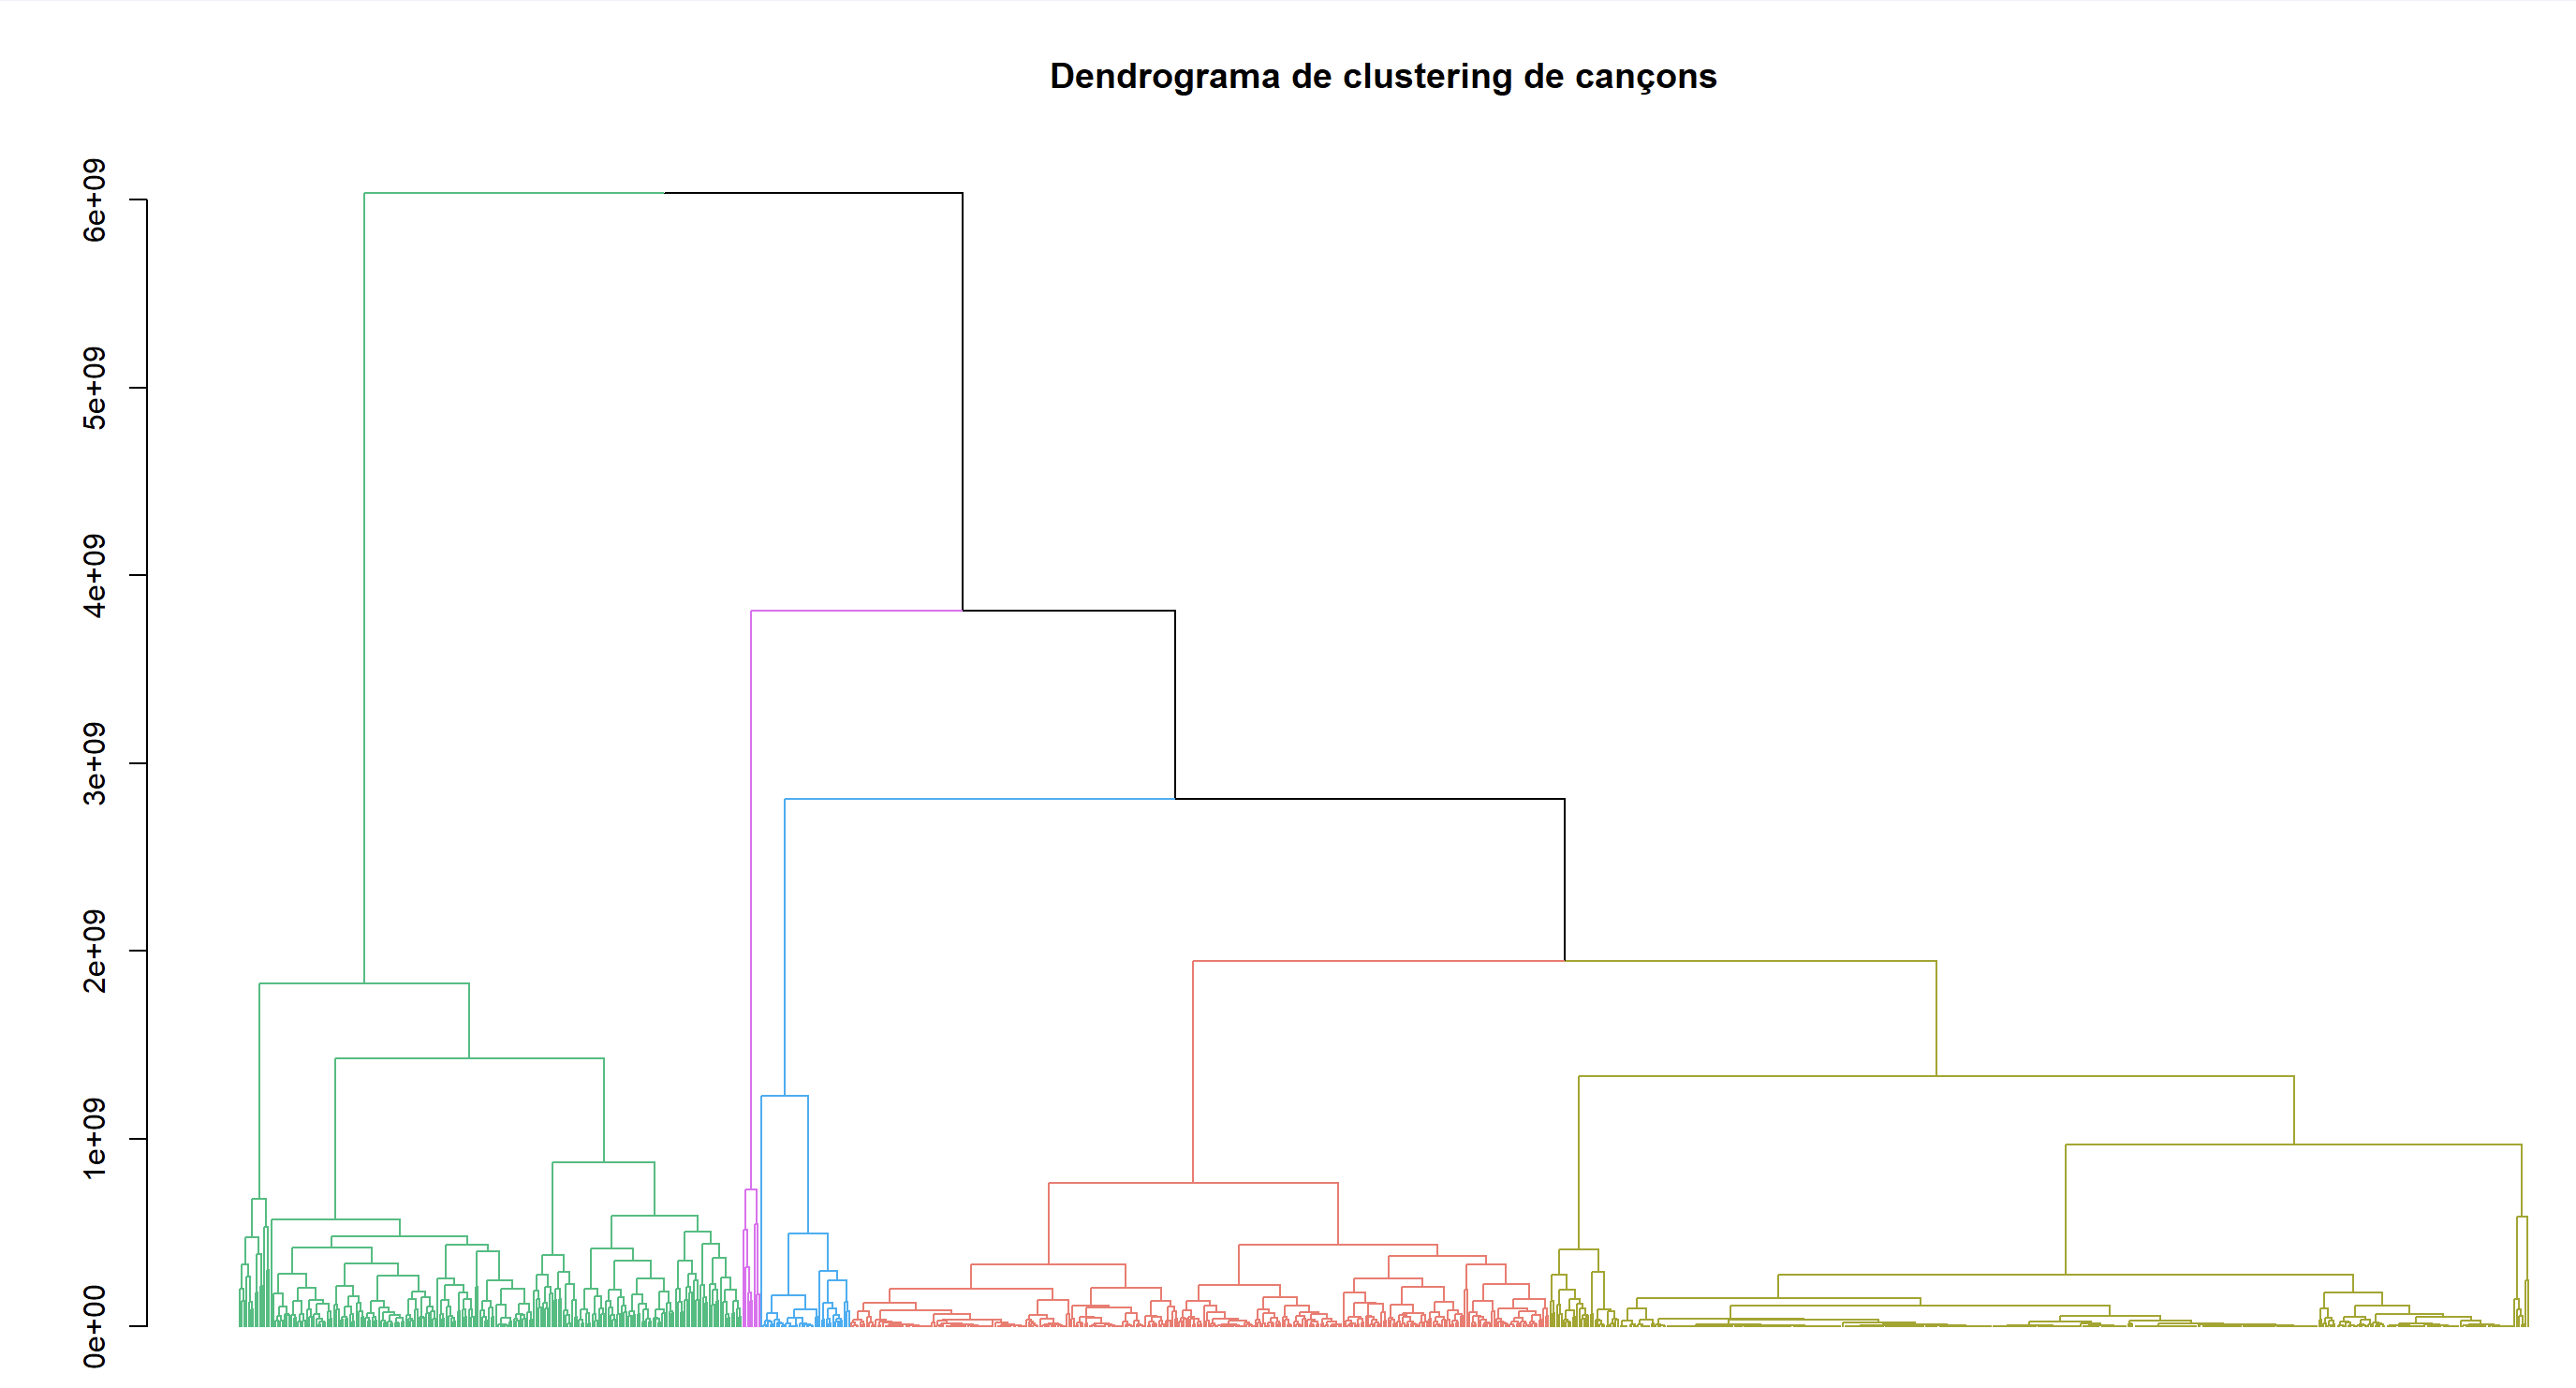
\includegraphics[width=\textwidth]{Images/4_clustering/time_series/dendrograma_colors.png}
    \caption{Dendrograma de cançons utilitzant distància \texttt{DTW} i mètode \texttt{ward.D2} amb els clústers colorejats ($k = 5$)}
    \label{fig:TS_dendrograma_colors}
\end{figure}

\subsubsection{Anàlisi dels resultats}

Amb els clústers ja establerts, s'ha procedit a realitzar un anàlisi detallat dels resultats amb l'objectiu d'interpretar i comprendre els motius subjacents que han conduït a la formació d'aquestes agrupacions

Les visualitzacions i anàlisis post-clústering, com ara la comparació entre els clústers i la durada mitjana de les cançons per cada agrupació, ofereixen una perspectiva més profunda permetent descobrir patrons amagats que ajudin a entendre millor la situació musical de l'aplicació.

Pel que fa a la figura \ref{fig:TS_tsclust_sc} podem observar les evolucions de les reproduccions per a cada clúster al llarg del temps.  Simplement al fer una breu ullada ja podem veure, més o menys, com estan distribuïdes les cançons. \\

\begin{itemize}
    \item \textbf{Clúster 1:} Aquest grup mostra un patró consistent en la quantitat de \textit{streams} amb un alt nivell de superposició de les sèries alhora que allargada, indicant una quantitat de streams sostinguda.
    
    \item \textbf{Clúster 2:} Aquest clúster presenta uns pics molt marcats al llarg dels anys indicant èxit ocasionalment que podria ser a causa de promocions o esdeveniments o inclús d'altres aplicacions que tenen molt poder d'influència com ara \textit{TikTok}. Cal recordar que la majoria de cançons es troben en aquest grup, i en aquests pics no s'hi veuen moltes cançons, de manera que hi ha una gran quantitat de cançons (les que no formen els pics) que no són tan populars i conformen la majoria del clúster.
    
    \item \textbf{Clúster 3:} Aquesta classe és molt similar al primer clúster però amb una diferència més significativa en les variacions entre cançons, encara que segueixen tenint una popularitat allargada. A més, els valors màxims són considerablement més alts que els del clúster 1, de manera que segurament hi ha cançons més populars en aquest clúster.
    
    \item \textbf{Clúster 4:} En aquest grup trobem les cançons que eren populars a l'inici de la creació del \textit{dataset} però que ràpidament van perdre l'interès, possiblement \textit{hits} d'aquella temporada. Cal mencionar com ja s'ha vist anteriorment que aquest clúster compta amb molt poques cançons, concretament 40.
    
    \item \textbf{Clúster 5:} Aquest grup, que és el més petit de tots, és el que té un període més llarg d'èxit i on les cançons tarden més en sortir del top després del pic. A més, els valors màxims són molt alts, de manera que segurament conté cançons molt populars.
\end{itemize}


\begin{figure}[H]
    \centering
    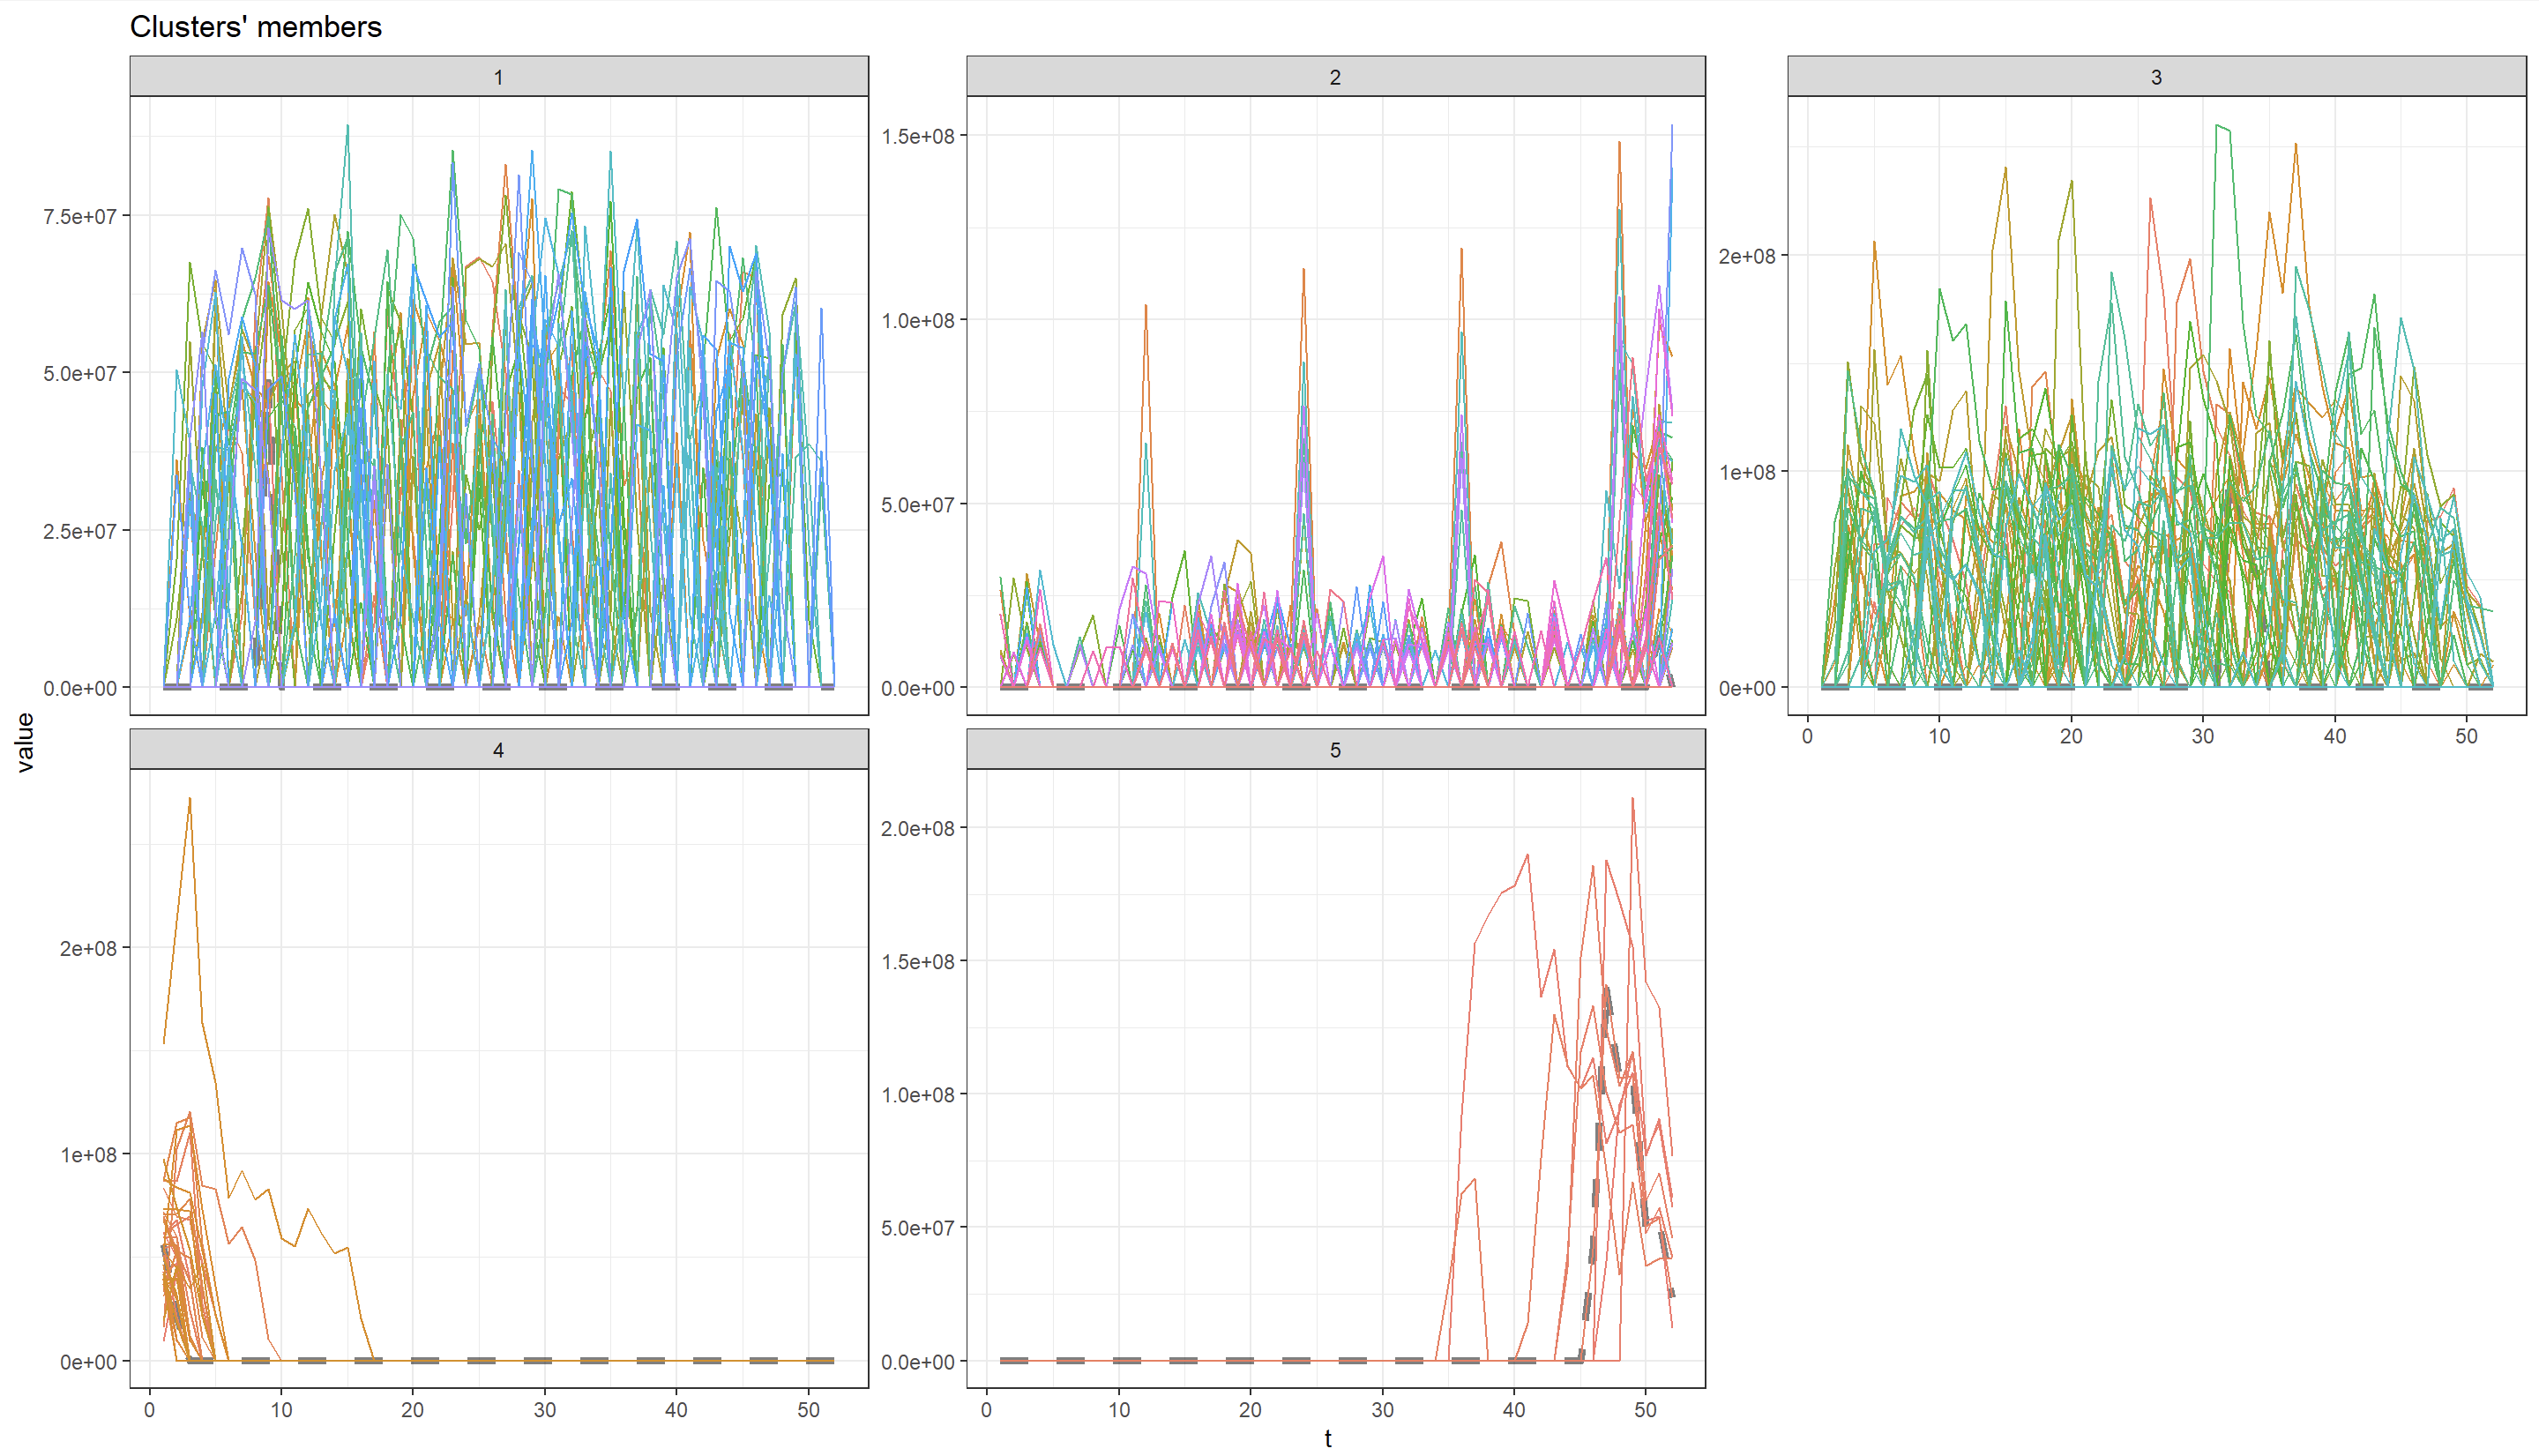
\includegraphics[width=0.8\textwidth]{Images/4_clustering/time_series/tsclust_sc.png}
    \caption{Gràfics de \textit{tsclust} amb l'evolució de streams per cada clúster}
    \label{fig:TS_tsclust_sc}
\end{figure}


Per poder acabar de visualitzar millor les conclusions anteriors s'ha creat un \textit{plot} per a cada classe representant l'evolució dels streams mensuals per cançó. Com podem veure en la figura \ref{fig:ts_clust_streams_month_cluster}, és molt similar a l'anterior però ens permet entendre millor les distribucions de les sèries. 

Tal i com s'ha mencionat, es pot mencionar que la diferència principal entre els clústers 1 i 3 és que aquests últims són bastant més populars alhora que la variància de streams és major entre cançons. També podem confirmar els forts pics espontanis del grup 2 i la major durada i gran popularitat de l'últim clúster (el 5).

A més, es pot veure com el clúster 3 (que conté les cançons que són generalment més populars) té una falta de cançons a l'inici i al final de la línia temporal. Això sembla justificar que el clúster 4 (amb nivells de popularitat semblants al grup 3) és el que conté les primeres cançons que haurien d'anar al clúster 3 (segurament separades pel fet de que han estat ``tallades'' per l'inici de la línia temporal, de manera que la seva sèrie temporal té una forma diferent); mentre que les cançons del clúster 5 semblen ser les cançons populars que haurien de correspondre al clúster 3, i les menys populars semblen haver anat al clúster 2 (degut a l'increment de reproduccions en aquest clúster al final de la seva línia temporal).

\begin{figure}[H]
    \centering
    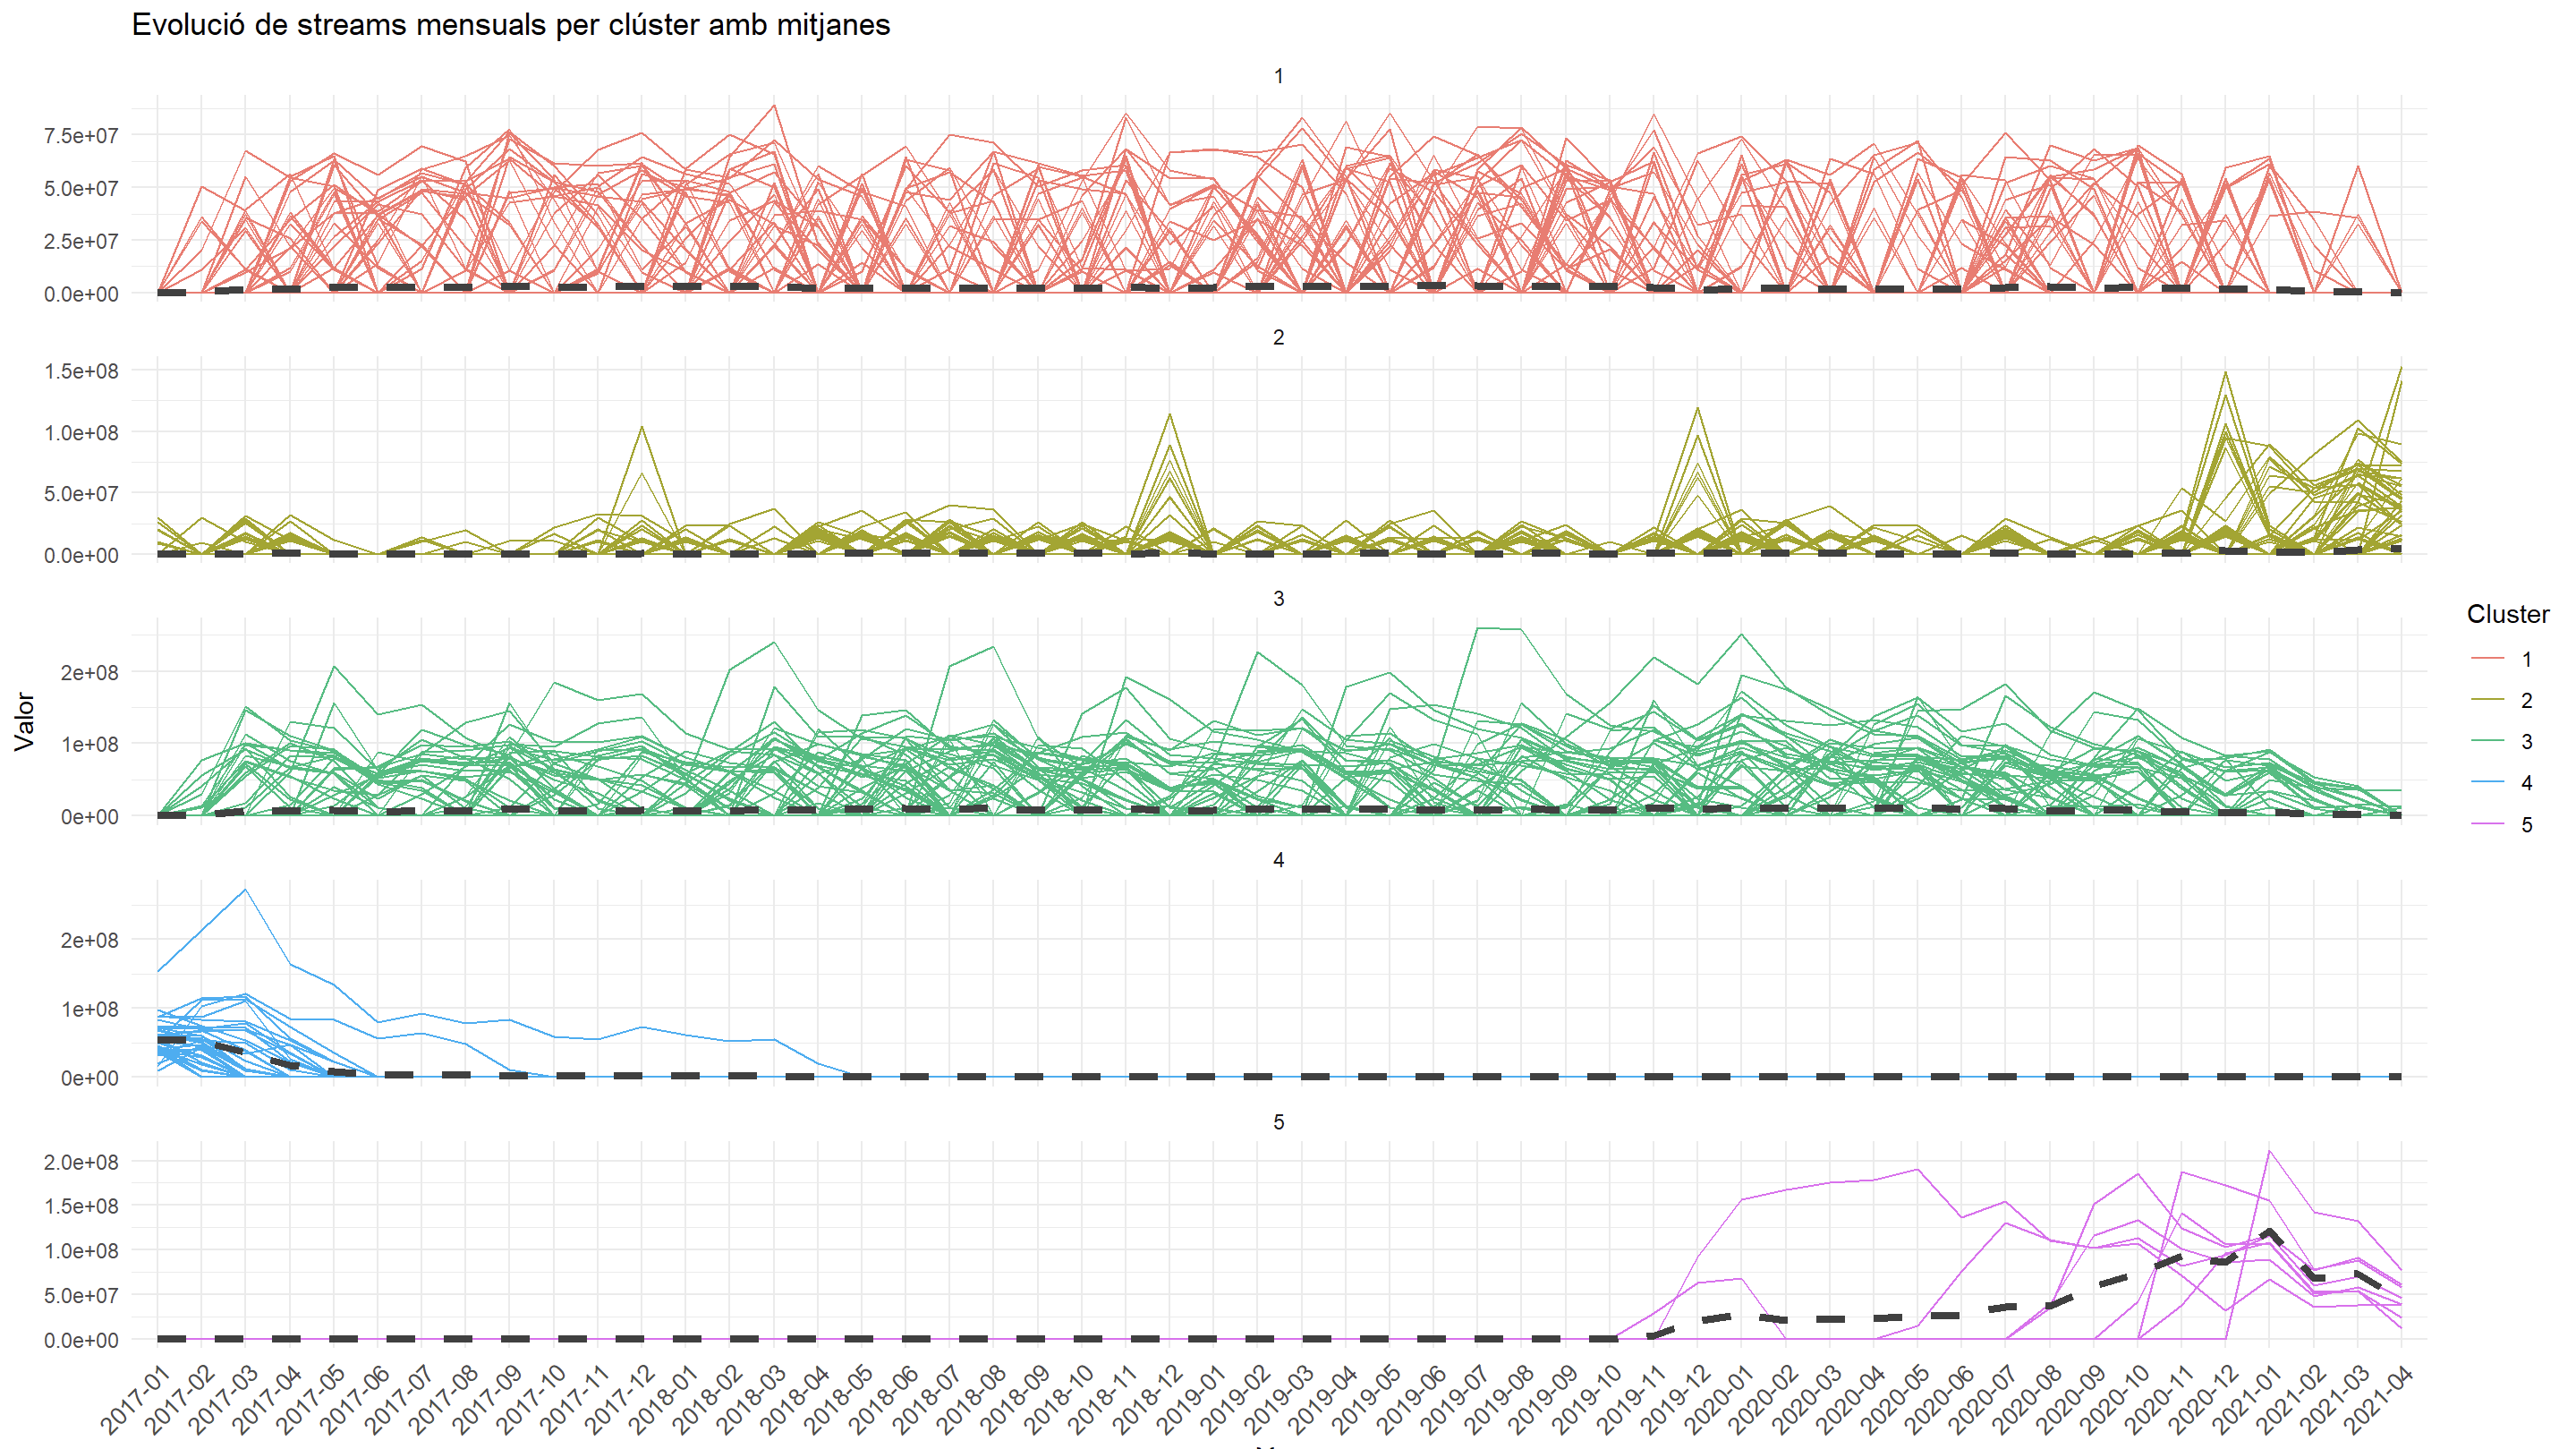
\includegraphics[width=0.8\textwidth]{Images/4_clustering/time_series/streams_cada_mes_per_cluster_amb_mitjana.png}
    \caption{Gràfics de l'evolució de les streams per a cada cançó dins de cada clúster}
    \label{fig:ts_clust_streams_month_cluster}
\end{figure}

Després d'analitzar aquestes sèries s'ha considerat important seguir l'estudi observant la mitjana de mesos actius de les cançons de cada grup indicant-nos així quins clústers contenen els èxits més prolongats i confirmant les conclusions anteriors.

En el primer \textit{barplot} \ref{fig:TS_barplot_mitjanes_mesos_actius} mostra la mitjana de mesos actius per clúster on es pot observar que el clúster 5, que és el més petit, conté les cançons que mantenen la popularitat constant durant el període de temps més llarg. El segon clúster que compleix això és el 3, com ja s'havia observat en l'anàlisi previ. 

Si ens fixem en el \textit{boxplot} \ref{fig:TS_boxplot_mesos_actius} podem observar i confirmar l'espontaneïtat de la classe 2 on pràcticament totes les cançons duren un sol mes en el top, encara s'hi poden observar \textit{outliers}.

\begin{figure}[H]
    \centering
    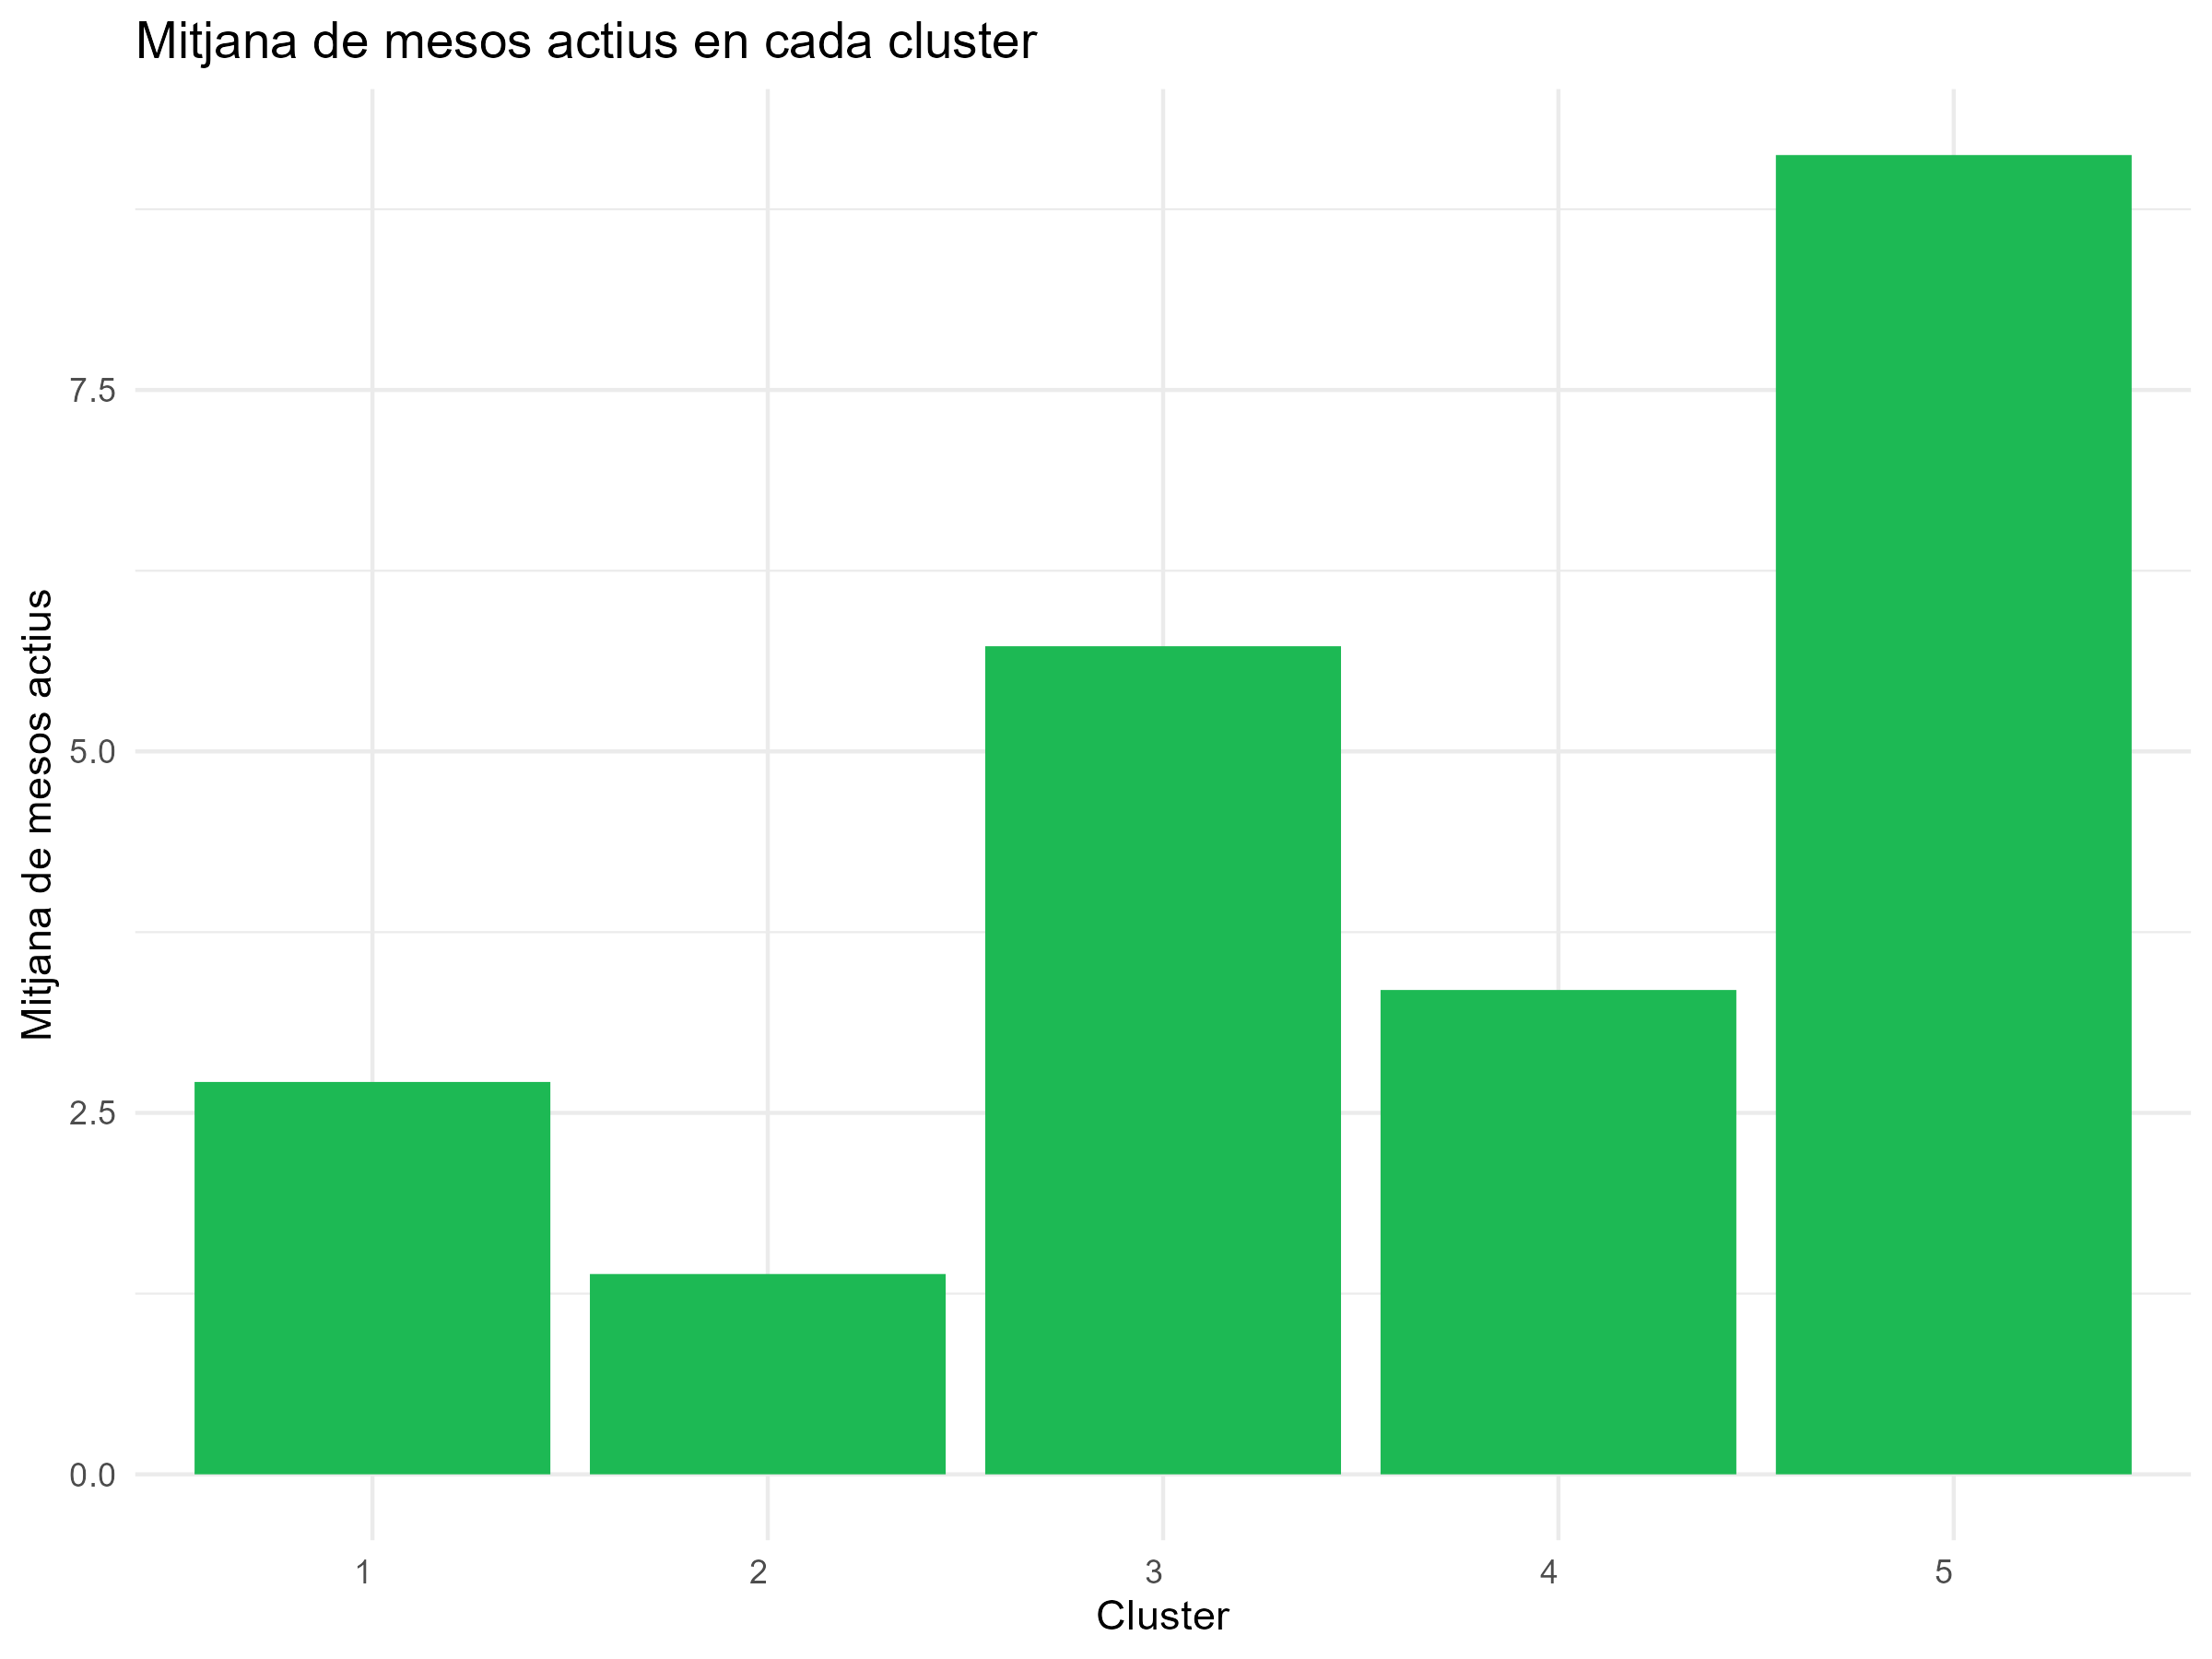
\includegraphics[width=0.8\textwidth]{Images/4_clustering/time_series/barplot_mitjanes_mesos_actius.png}
    \caption{Barplot de la mitjana de mesos actius de les cançons per cada clúster}
    \label{fig:TS_barplot_mitjanes_mesos_actius}
\end{figure}

\begin{figure}[H]
    \centering
    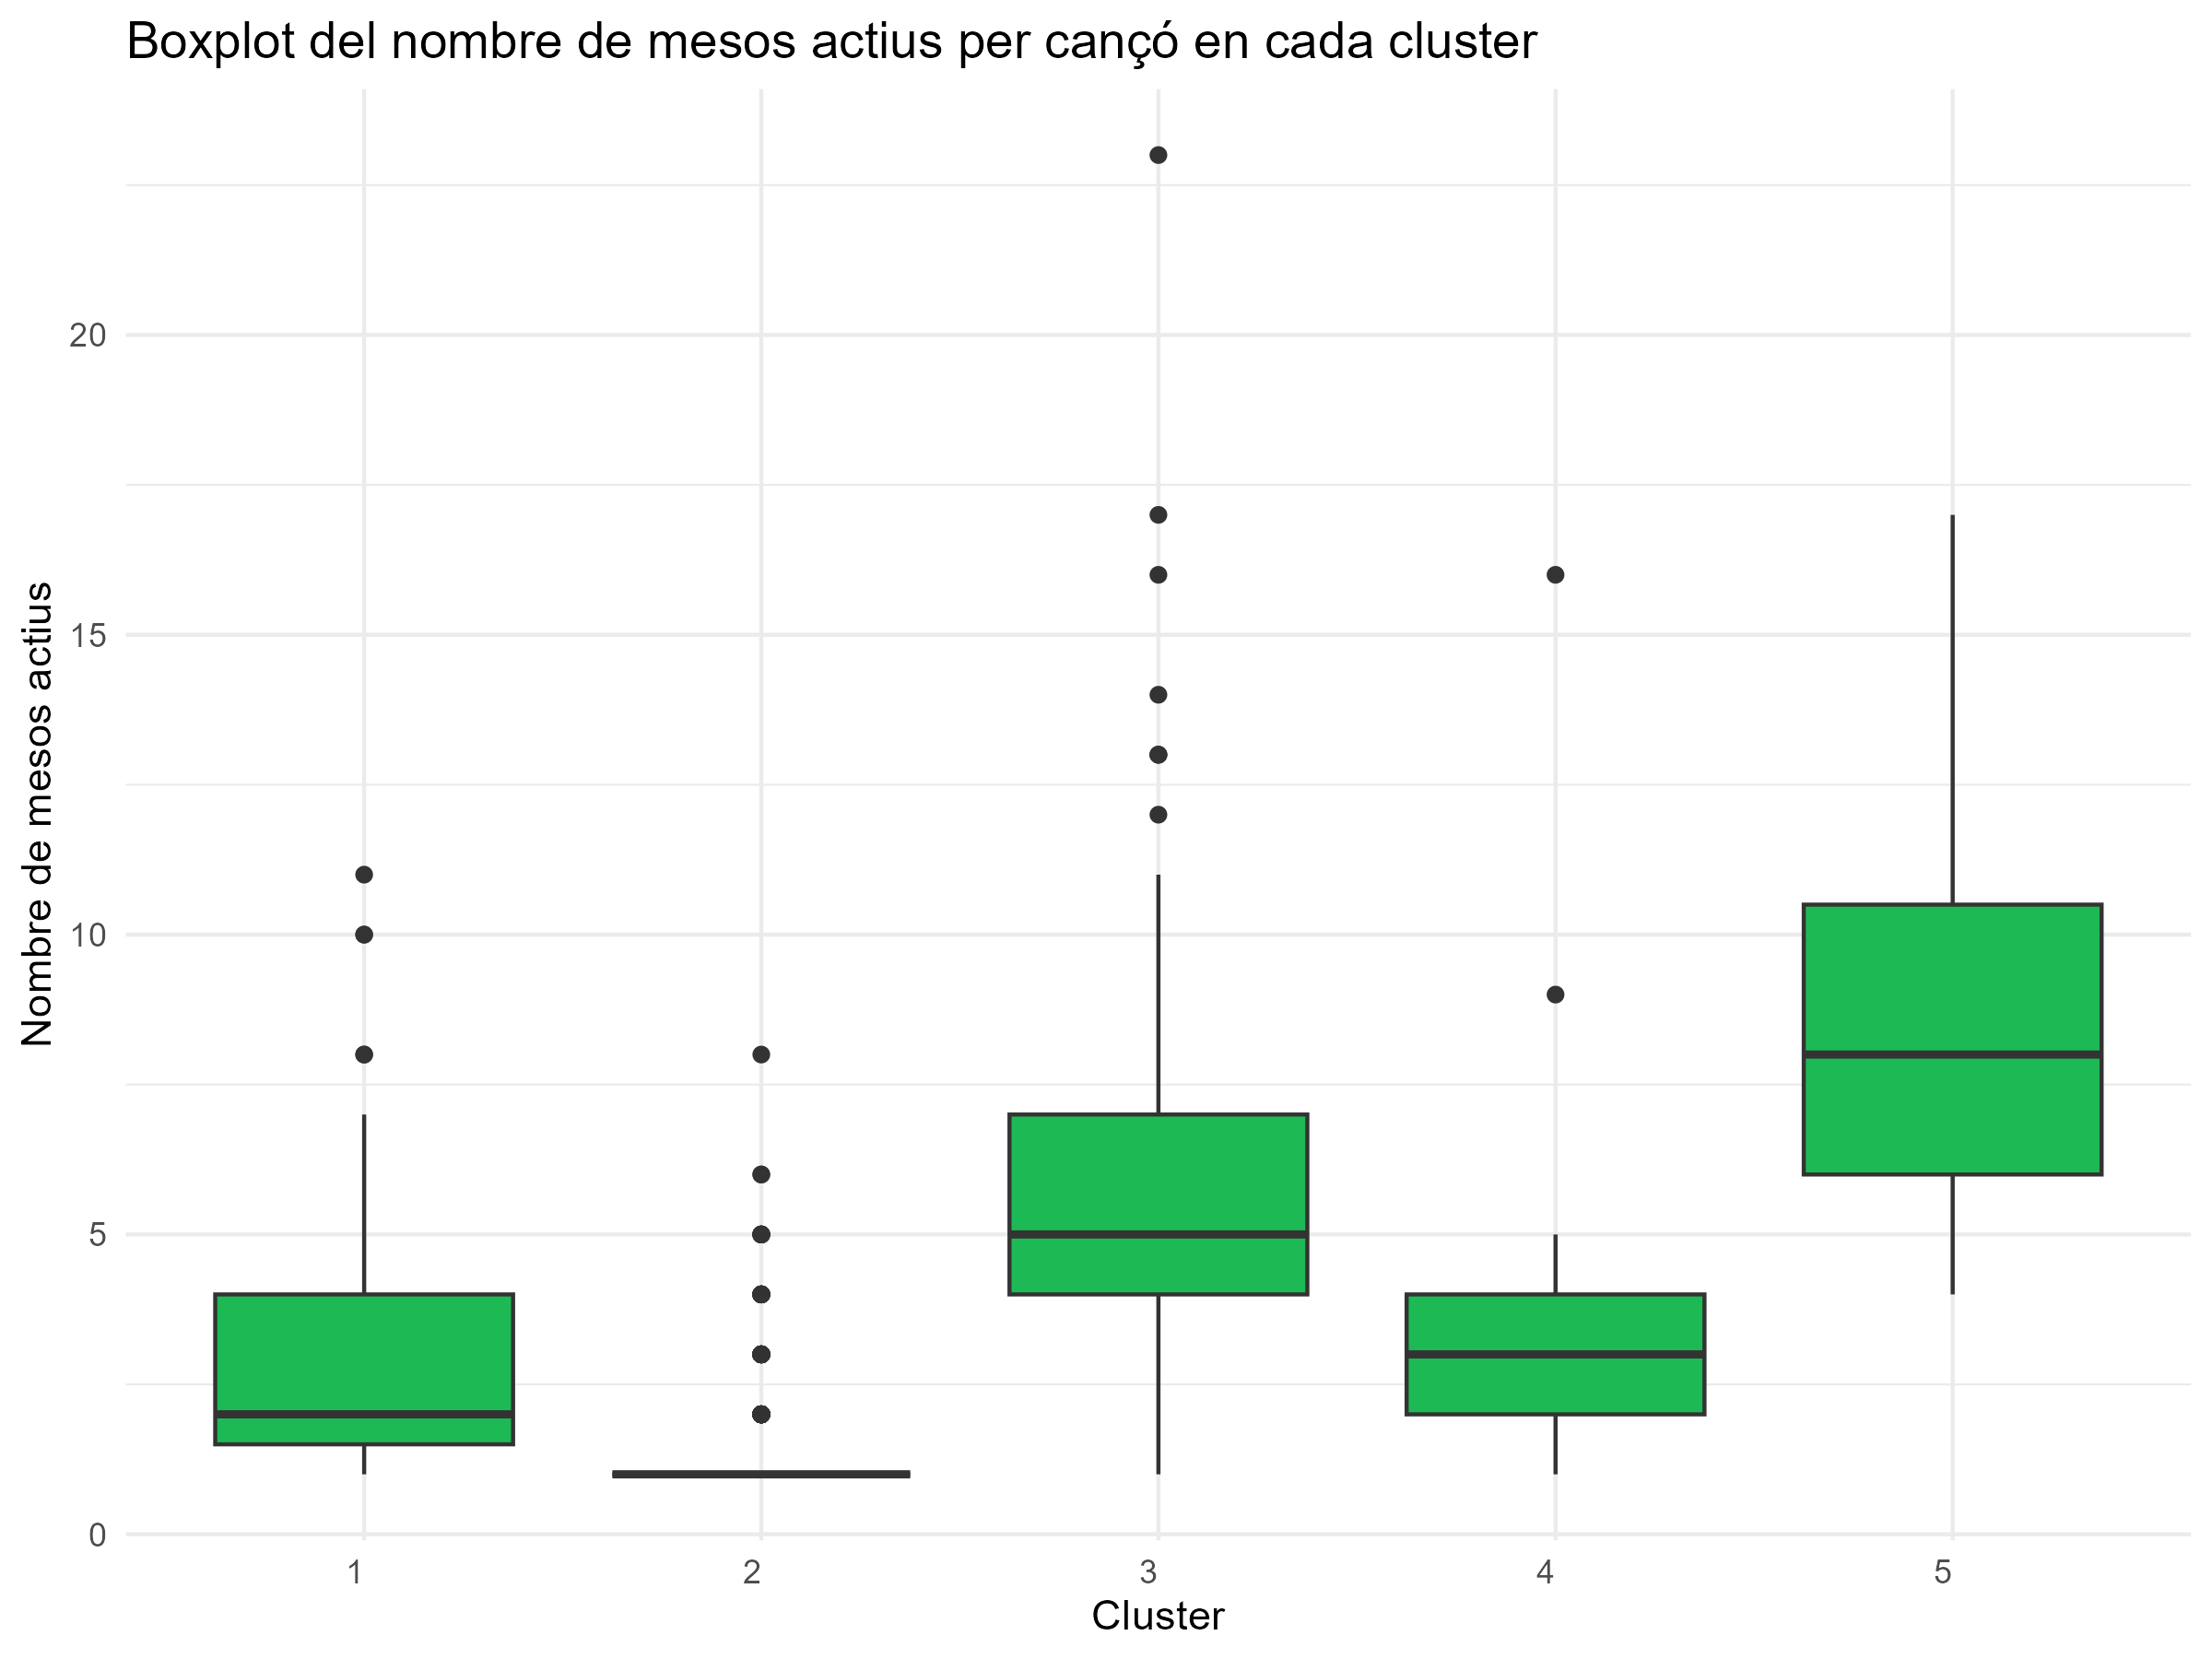
\includegraphics[width=0.8\textwidth]{Images/4_clustering/time_series/boxplot_mesos_actius.png}
    \caption{Boxplot de la distribució de mesos actius de les cançons per cada clúster}
    \label{fig:TS_boxplot_mesos_actius}
\end{figure}

Per poder comprendre millor els clústers, s'ha realitzat un gràfic agrupat per mesos per poder veure si hi ha algun patró estacional ens els diferents clústers. Com es pot veure en la figura \ref{fig:TS_evol_streams_per_mes_i_cluster}, aparentment en els 3 primers clústers no hi ha gaire diferència entre mesos, tan sols es podria comentar un lleuger augment de reproduccions durant els mesos d'estiu.

Pel que fa als clústers 4 i 5, com ja s'ha mencionat prèviament corresponen a les cançons que inicien i acaben els tops en el dataset. Com que els primers valors es van mesurar al gener de 2017, podem veure que en el clúster número 4 (color blau) durant els primers mesos de l'any té moltes streams però a partir del juny ja pràcticament no en té. Per altra banda, el clúster 5, concentra els seus streams durant els mesos d'hivern, ja que és quan hi ha els últims valors mesurats del dataset.

\begin{figure}[H]
    \centering
    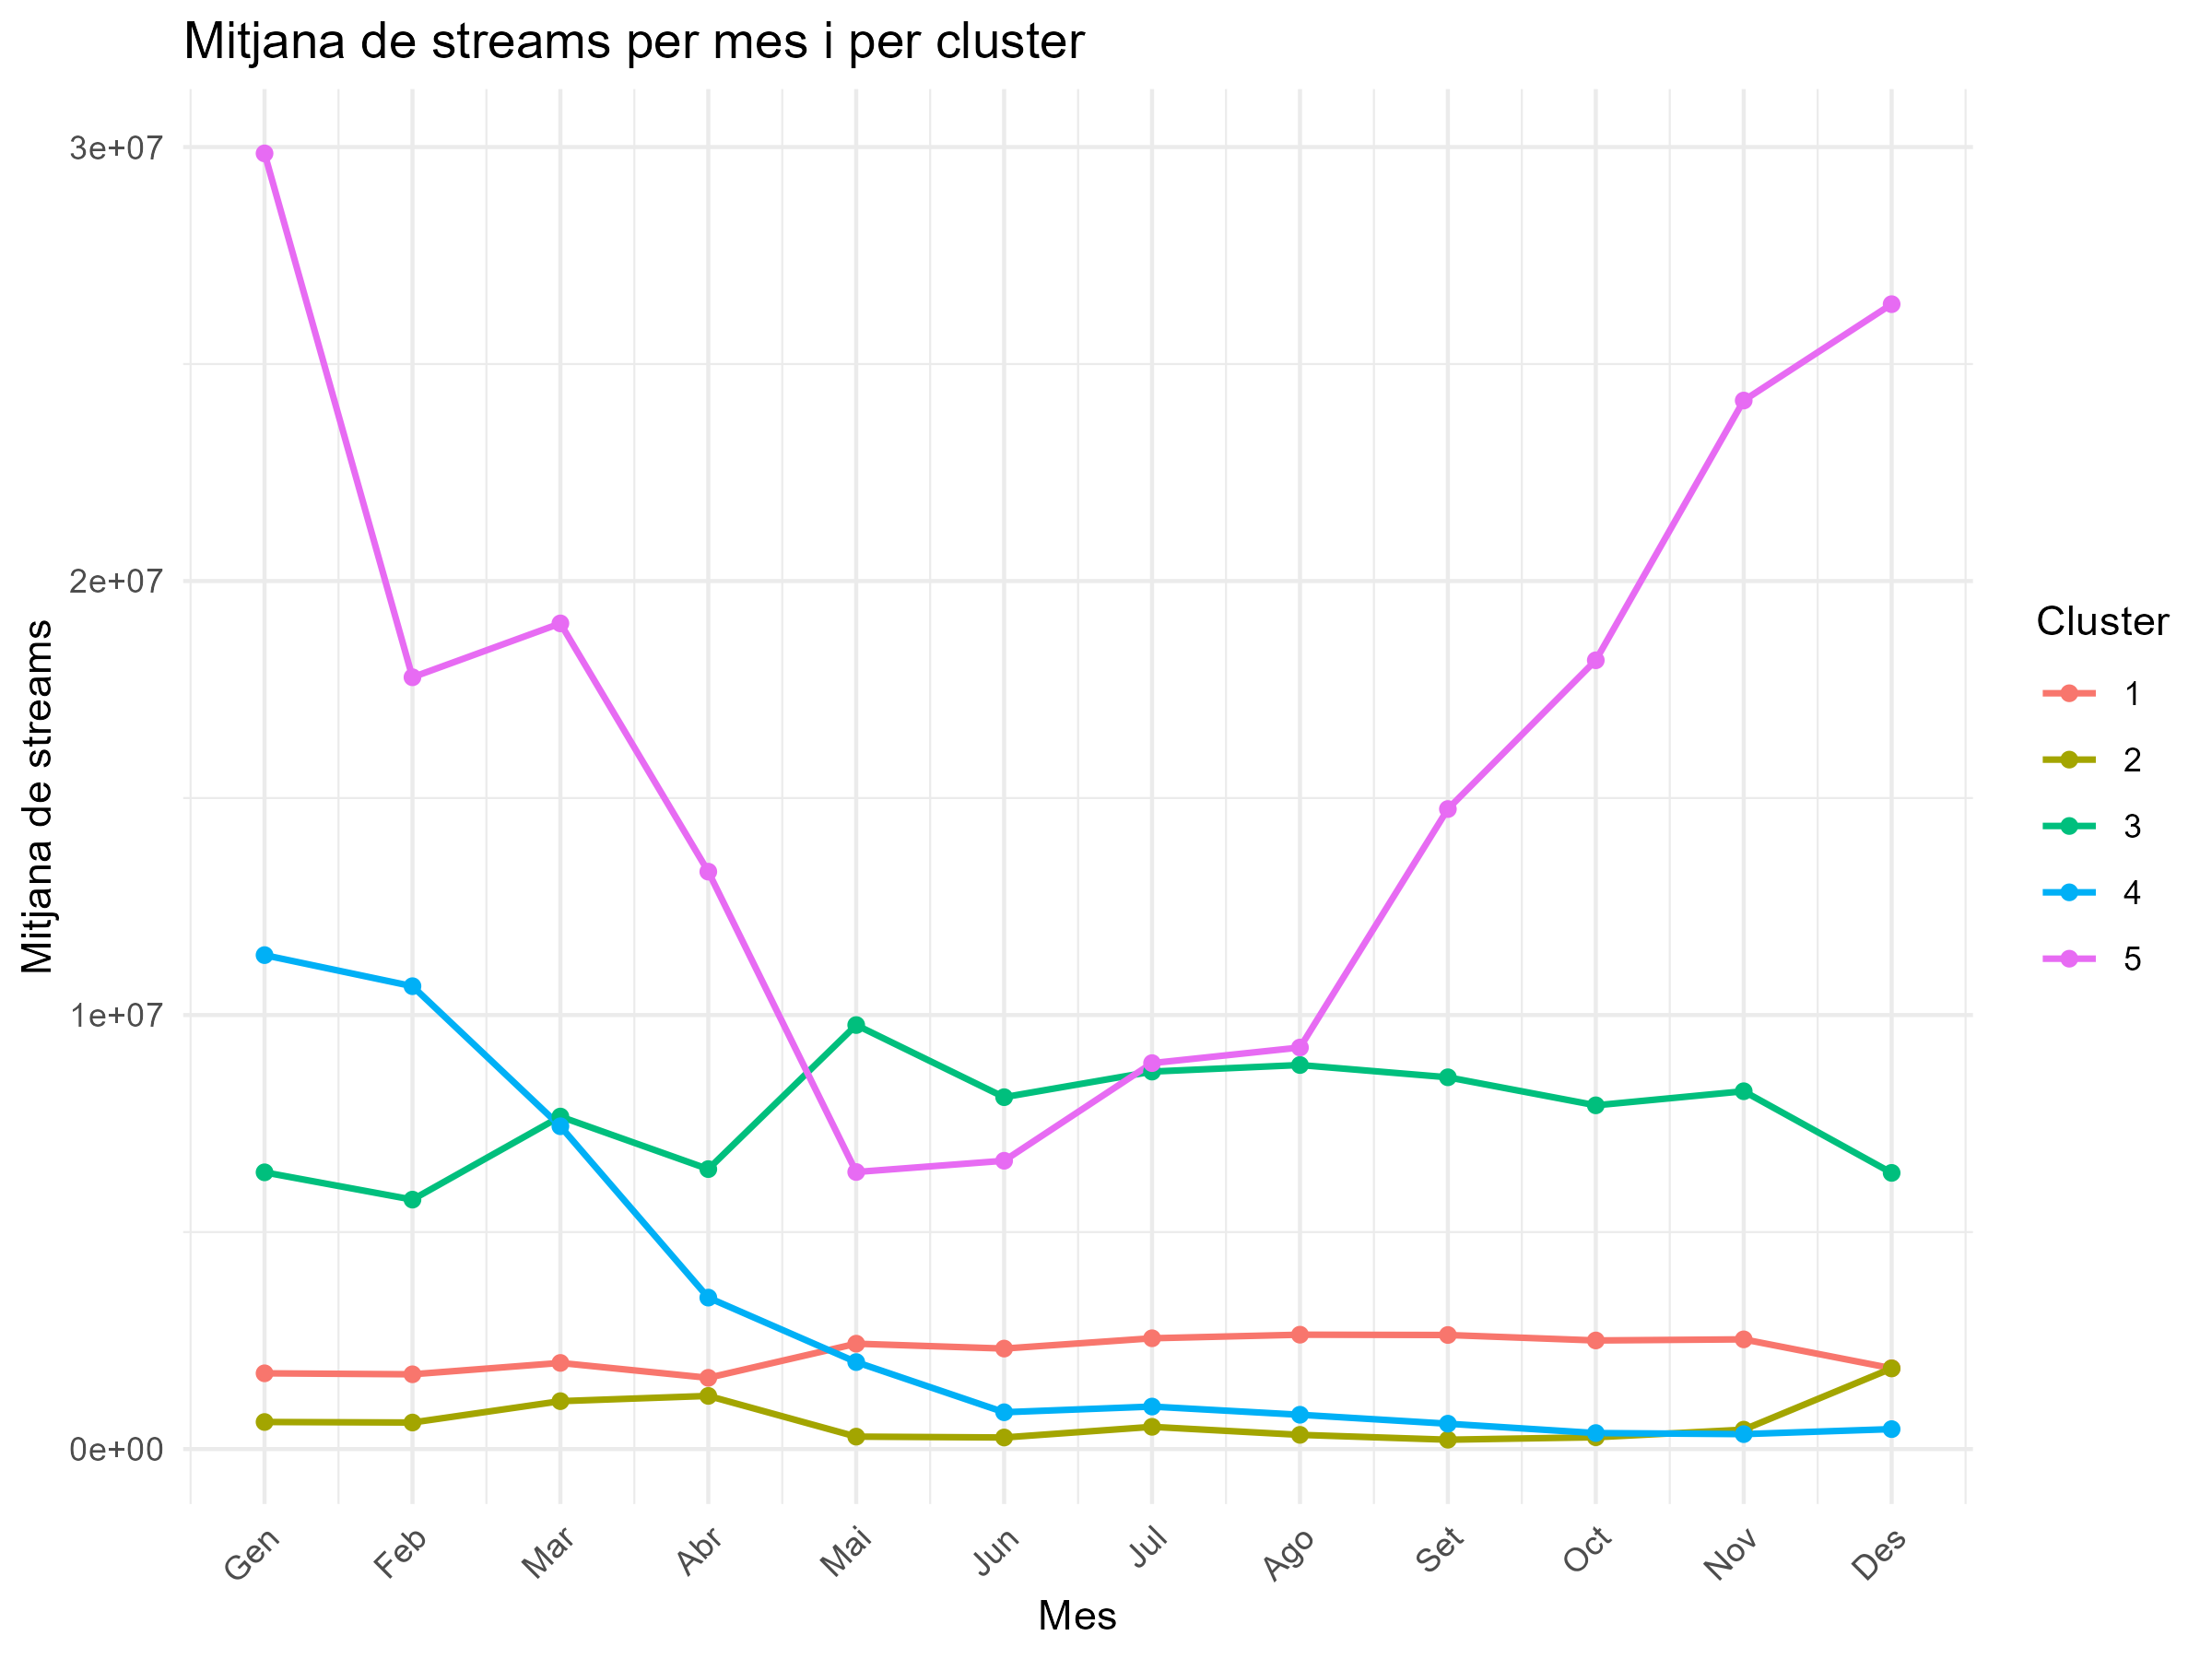
\includegraphics[width=0.8\textwidth]{Images/4_clustering/time_series/evol_streams_per_mes_i_cluster.png}
    \caption{Gràfic amb la mitjana dels streams de cada clúster en funció dels mesos}
    \label{fig:TS_evol_streams_per_mes_i_cluster}
\end{figure}

Com s'ha mencionat prèviament, quan una cançó no apareix en el top 40 durant tot el mes, el seu valor de streams s'ha considerat 0. Això implica que en el gràfic de la figura \ref{fig:TS_evol_streams_per_mes_i_cluster} les mitjanes inclouen molts zeros, de manera que els resultats poden estar condicionats per la quantitat de mesos actius de cada clúster (que ja s'ha vist prèviament). Per tal de veure l'evolució de les mitjanes de streams al llarg dels mesos només tenint en compte quan les cançons estan al top 40 (sense considerar els zeros) s'ha creat el gràfic de la figura \ref{fig:TS_evol_streams_per_mes_i_cluster_no_zeros}. Com es pot veure, el canvi és important, i ara s'aprecia com, per exemple, el clúster 2 té un increment de streams en el mes de desembre (tal i com es veia en els pics mencionats prèviament), però durant tot i així té una mitjana de streams baixa al llarg de tot l'any. Pel que fa al clúster 1, és el més estable de tots i no conté cançons gaire populars. Per altra banda, el clúster 4 té un increment important de streams durant els mesos d'estiu i també al desembre, mantenint en general un nivell mig de popularitat en les seves cançons (tot i que s'ha de tenir en compte que conté cançons només populars al principi del registre, dem manera que en aquest gràfic no s'ha de tenir gaire en compte la seva estacionalitat). Pel que fa al clúster 3, té en general una popularitat alta durant totes les èpoques, sense grans diferències entre elles. Finalment, el clúster oscil·la molt (segurament degut a que només conté 8 cançons) i té una popularitat molt alta en tots els mesos, però especialment durant els primers mesos d'estiu, a la tardor i al gener (tot i que no es pot estudiar gaire la seva estacionalitat degut a que conté cançons només del final del registre).

\begin{figure}[H]
    \centering
    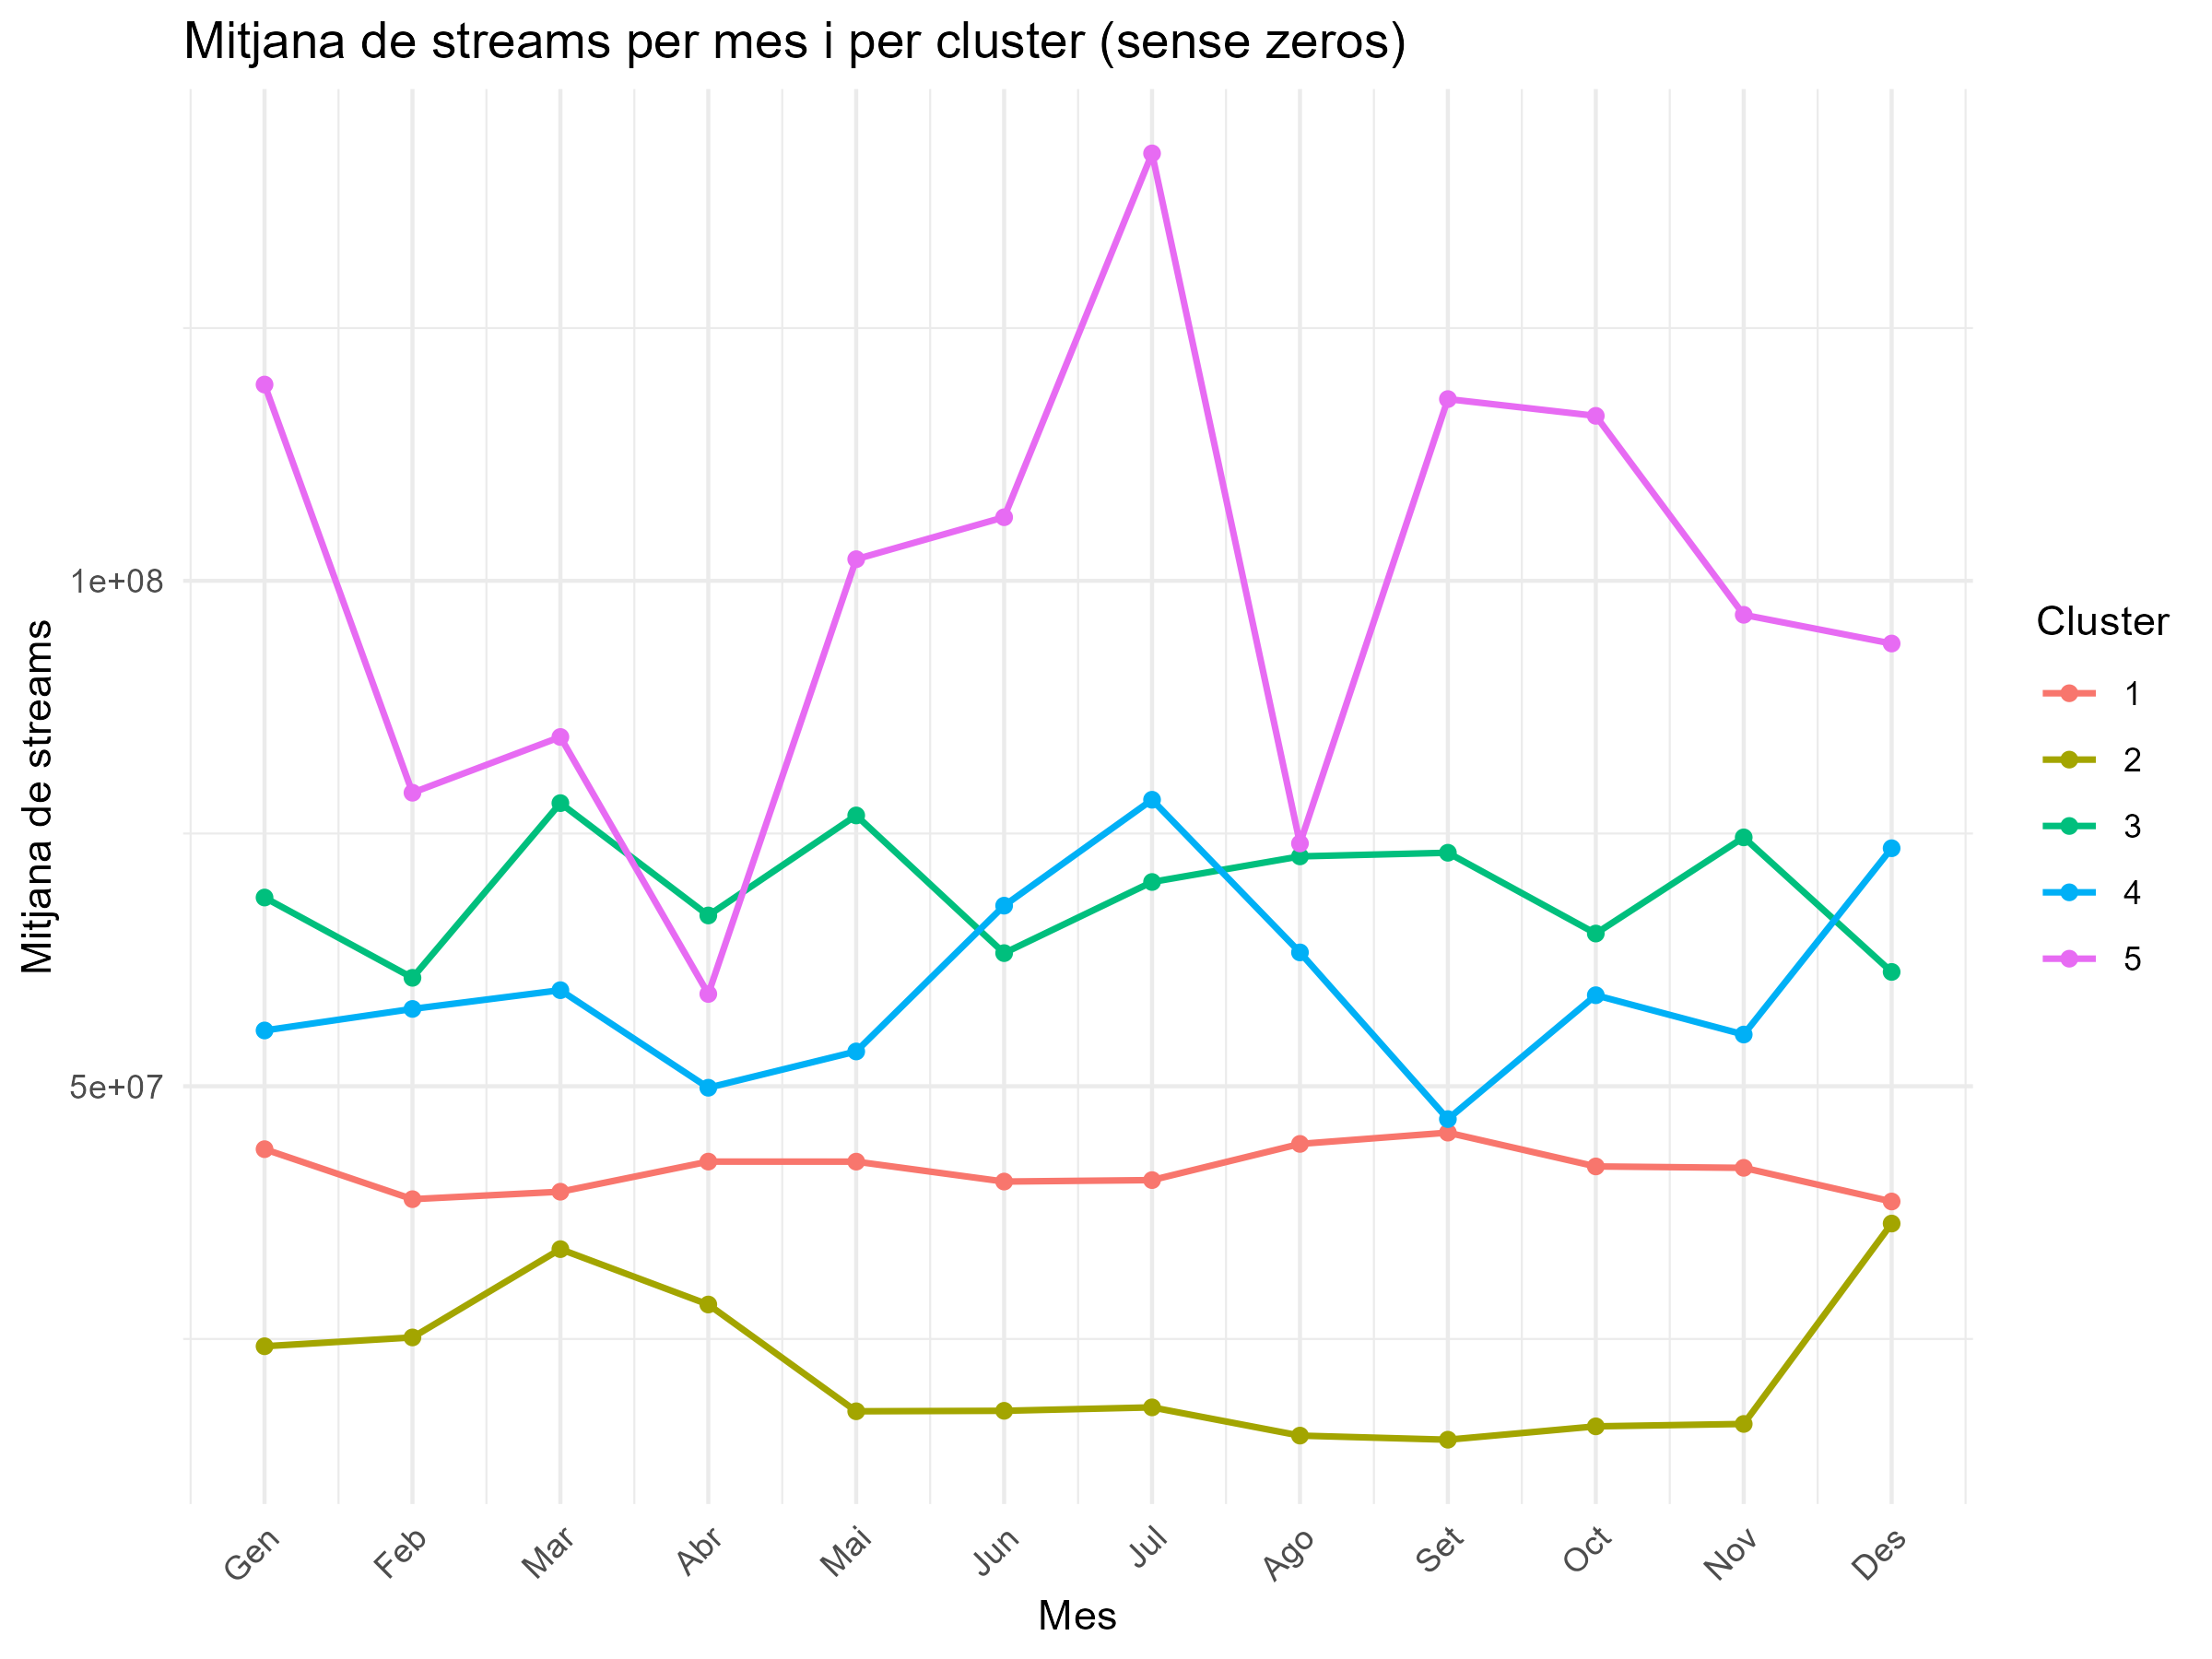
\includegraphics[width=0.8\textwidth]{Images/4_clustering/time_series/evol_streams_per_mes_i_cluster_no_0.png}
    \caption{Gràfic amb l'evolució de la mitjana de streams (sense considerar quan el valor és zero) de cada clúster en funció dels mesos}
    \label{fig:TS_evol_streams_per_mes_i_cluster_no_zeros}
\end{figure}

Amb tot el que s'ha vist, les conclusions són similars a les que s'han mencionat en l'anàlisi inicial. S'ha de tenir en compte que realizar un \textit{profiling} d'aquests clústers no és especialment fàcil, ja que s'han realitzat només tenint en compte el component temporal de streams en la base de dades, ignorant totes les altres variables.

Resumidament, es poden concloure les següents descripcions pels 5 clústers:
\begin{itemize}
    \item \textbf{Clúster 1:} Cançons poc populars i amb una durada no gaire sostinguda al llarg dels mesos.
    
    \item \textbf{Clúster 2:} El grup amb les cançons generalment menys populars i espontànies, tot i que amb alguns hits puntuals al desembre, que s'ha analitzat i, curiosament, no corresponen a cançons de nadal. Sembla contenir les cançons finals no tant populars del clúster 3.
    
    \item \textbf{Clúster 3:} Les cançons generalment més populars, sense ser les més antigues ni les més recents, i bastant sostingudes al llarg dels mesos en el top 40.
    
    \item \textbf{Clúster 4:} Cançons una mica menys populars que en el grup 3 i menys sostingudes, probablement perquè es concentren en els primers anys de la base de dades. Semblen ser les cançons inicials que manquen al clúster 3.
    
    \item \textbf{Clúster 5:} Les cançons més populars, més sostingudes al llarg dels mesos i que encara es trobaven presents al final del registre. Semblen ser les cançons populars finals que manquen al clúster 3.
\end{itemize}

Cal mencionar que l'existència dels clústers 4 i 5 pot ser deguda a que es troben en els inicis/finals dels mesos comptabilitzats a la base de dades, de manera que la seva sèrie temporal probablement té una forma especial (retallada pels extrems) que ha provocat que la distància DTW els separi, resultant en els dos grups amb menys cançons (només 40 i 8).

A més, també es pot afegir que en la figura \ref{fig:TS_dendrograma_colors} es confirma que els clústers 1 i 2 són els més similars, la qual cosa es podia preveure degut a la poca quantitat de streams que comparteixen.


%\newpage
\section{Profiling}

Un cop hem utilitzat diferents tècniques de clustering per agrupar les nostres dades, escollint els hiperparàmetres, ara toca fer el profiling. El profiling ens servirà per analitzar els clústers formats durant el clustering jeràrquic i veure com s'han dividit les dades. Per realitzar això, utilitzarem una sèrie de tests d'hipòtesi i gràfiques diverses. També s'intentarà fer una comparació dels clústers que s'han format durant aquest quatrimestre als clústers que van sorgir a ME. Això ens permetrà veure si les noves variables que hem afegit a la base de dades han afectat a l'agrupació o no. 

Primer de tot, trobem interessant veure quantes mostres hi ha a cada un dels clústers. Com veiem a la figura \ref{fig:Cat_BarPlot_cluster_hier}, els 5 clústers escollits no tenen la mateixa mida. Els clústers 1, 2 i 4 tenen mida semblant. No obstant, el tercer clúster té una mida bastant superior als altres i el cinquè clúster no arriba a 1000 instàncies.

\begin{figure}[H] 
    \centering
    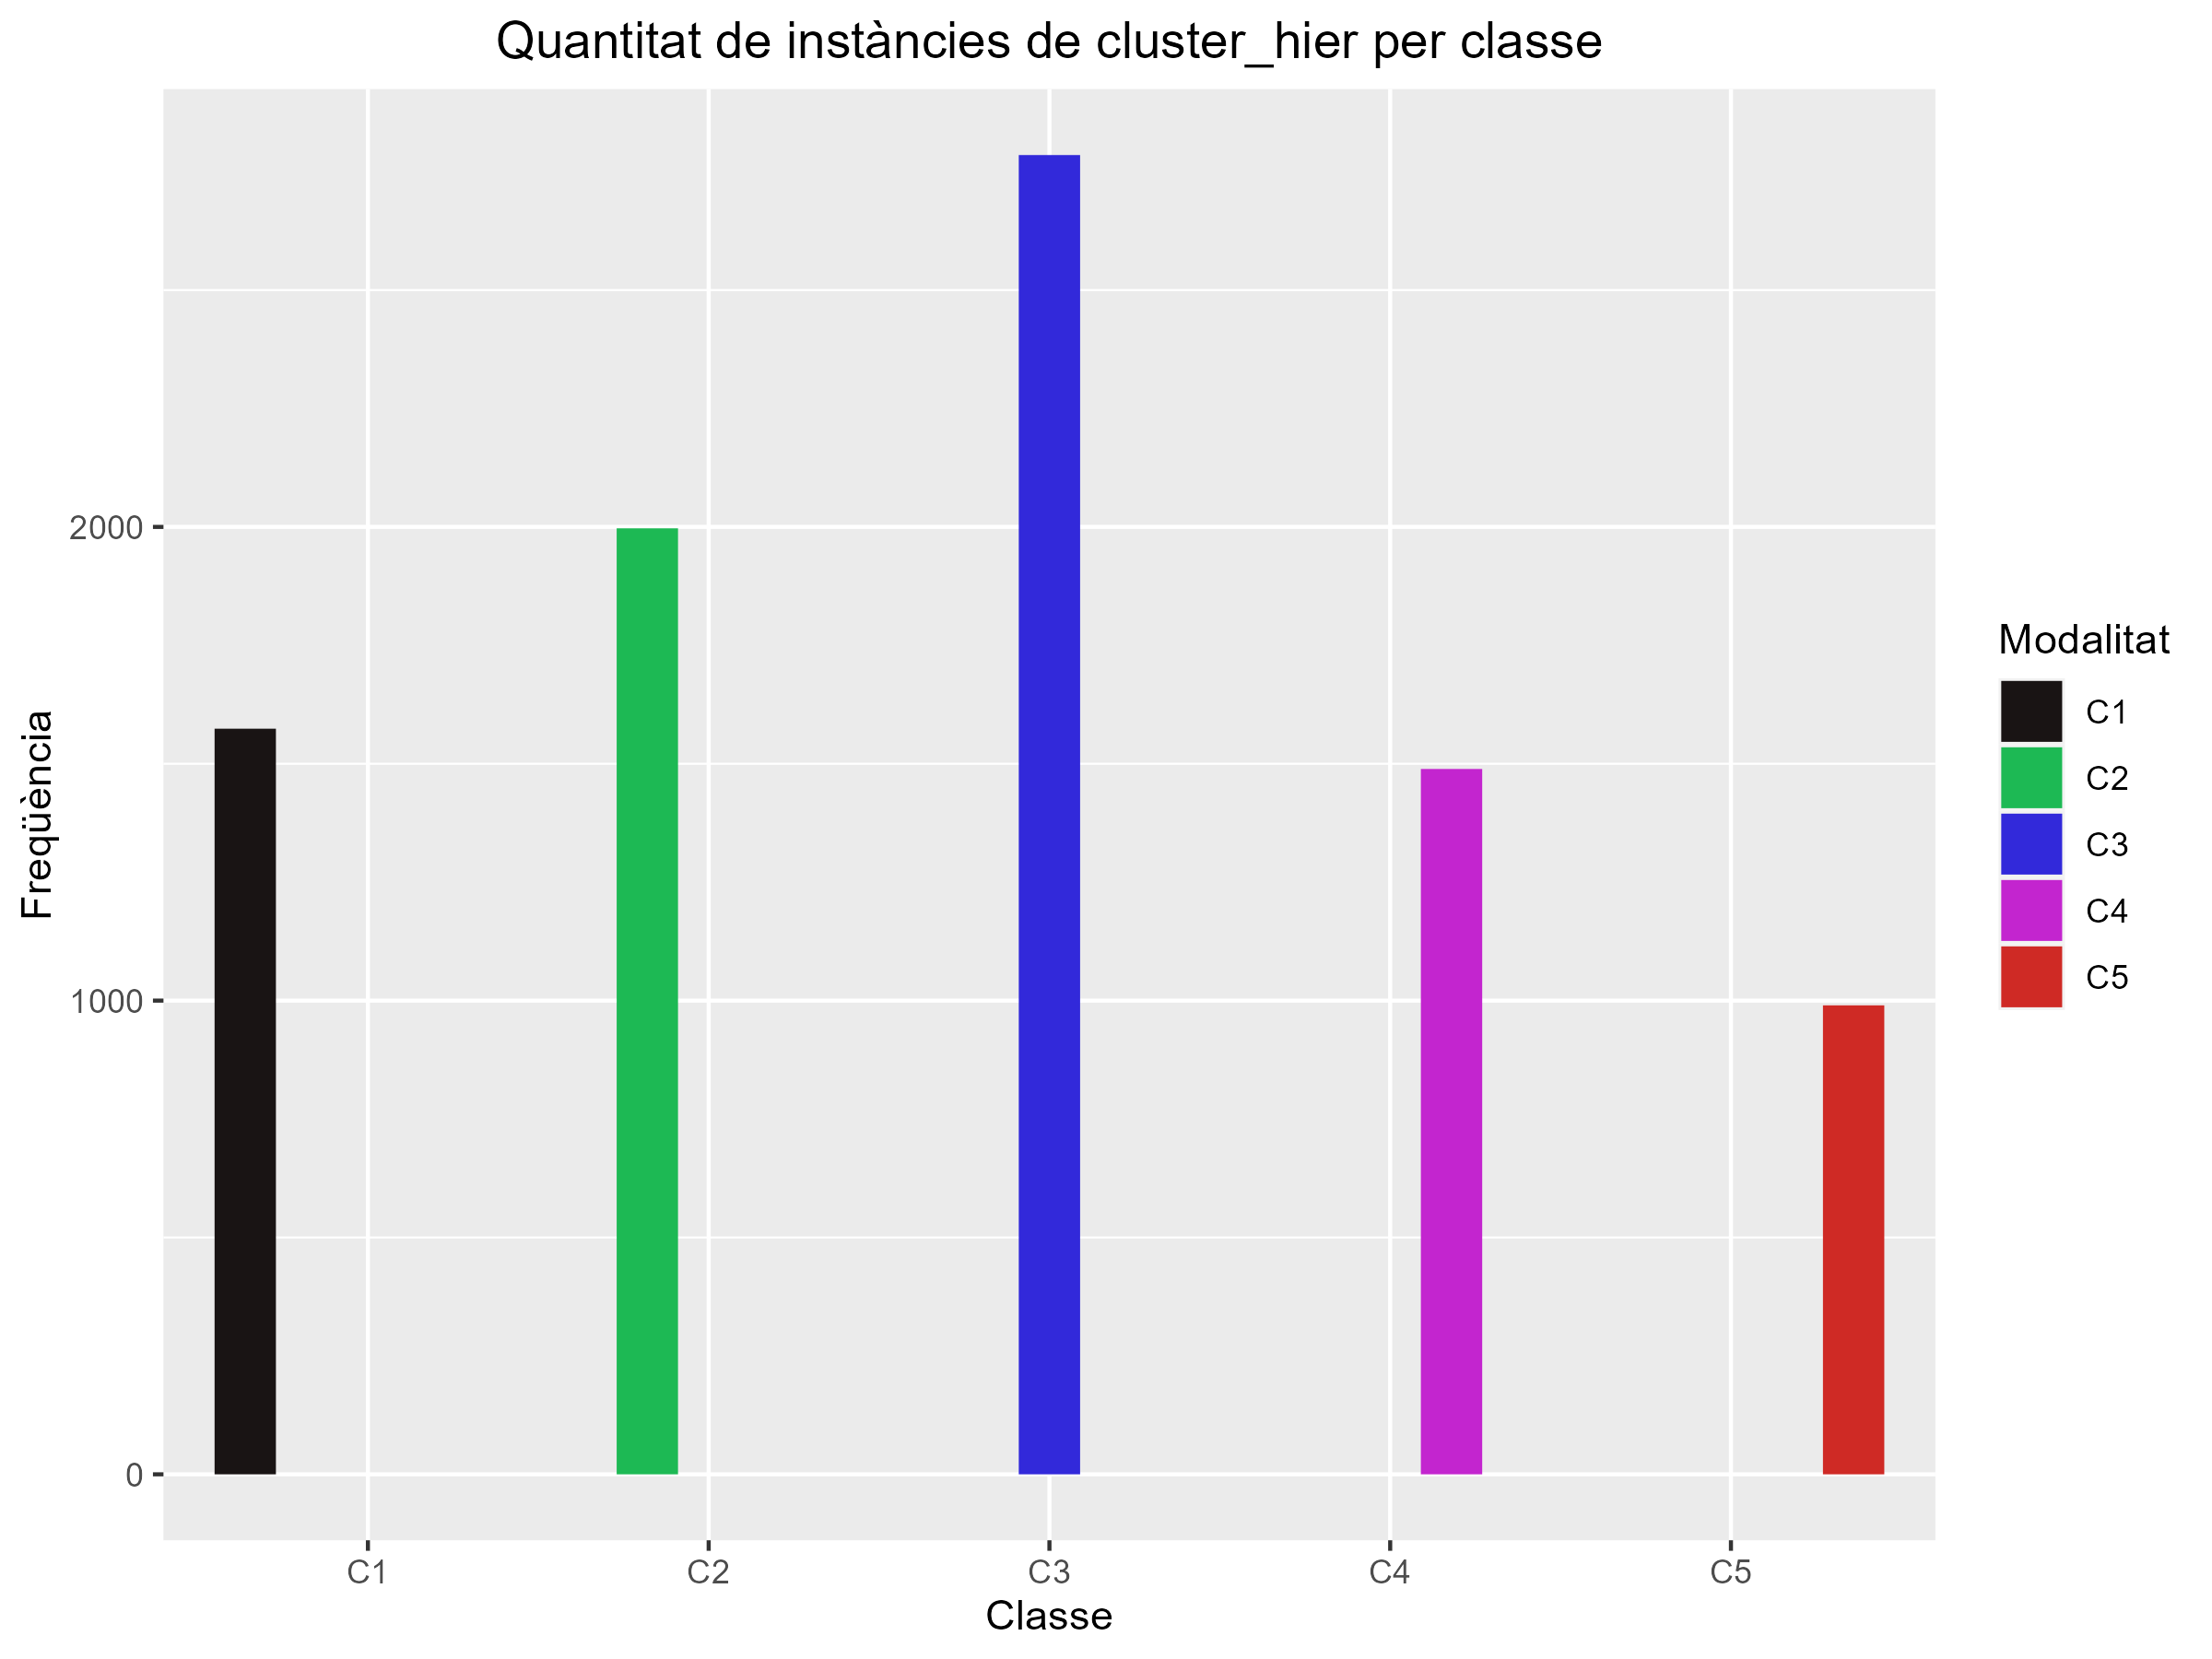
\includegraphics[width=0.7\textwidth]{Images/5_Profiling/categoriques/cat/Cat_BarPlot_cluster_hier.png}
    \caption{Barplot amb la quantitat d'instàncies per clúster}
    \label{fig:Cat_BarPlot_cluster_hier}
\end{figure}

És important, a l'hora de la visualització, tenir en compte que els gràfics de barres estan desbalancejat i que no afecti a la nostra anàlisi. 

\subsection{Variables numèriques}

En el cas de les numèriques, per veure si cada una de les variables és significativa en els clústers, utilitzarem test d'hipòtesi amb els quals ja estem familiaritzats. Farem servir el ANOVA, el Kruskal-Wallis i el t-test i els acompanyarem amb BarPlots i Boxplots per visualitzar les diferències.

El que fa l'ANOVA és comparar les mitjanes de cada variable numèrica en cada un dels clústers, amb això mira si hi ha una diferència significativa entre les mitjanes. La nostra hipòtesi nul·la és que no hi ha diferències significatives entre les mitjanes a cada classe, i la hipòtesi alternativa serà que almenys alguna de les mitjanes de la nostra variable numèrica és diferent depenent de les clases. 

Ja sabem que el test ANOVA assumeix que les nostres variables segueixen una distribució normal, però com el nostre dataset és superior a 100 mostres, segons el teorema del límit central, assumim que la distribució de les nostres variables s'assemblarà a una distribució normal per poder fer aquests tests. Tot i això, per si a cas, també es fa servir un altre test que en aquest cas no requereix que les seves variables sí que tinguin una distribució normal, que és el Kruskal-Wallis. Aquest test té com a objectiu comparar dues mostres, i saber si pertanyen a la mateixa població amb variàncies similars o les segves variàncies són significativament diferents. 

Finalment, també s'ha fet un t-test, que el que fa és comparar les mitjanes de les distribucions que tindrà cada variable dins de cadascun dels clústers amb la mitjana generat que té la variable. Per aquest test la nostra hipòtesi nul·la serà que les mitjanes de la distribució de la variable dins del clústers comparada amb la distribució de la variable total no són significativament diferents. 

Ara sí, podem començar a mirar variable per variable si aporten significativament al clustering format i si ho fan, en quina de les quatre classes està afectant més. En el cas de les numèriques, no s'han afegit noves variables durant el preprocessing, per tant, es faran els tests per les mateixes variables del quatrimestre passat però més tard ja mirarem si es fan coses similars o la formació dels clústers no té res a veure. 

\begin{figure}[H]
\centering
    \begin{minipage}{.49\textwidth}
        \centering
        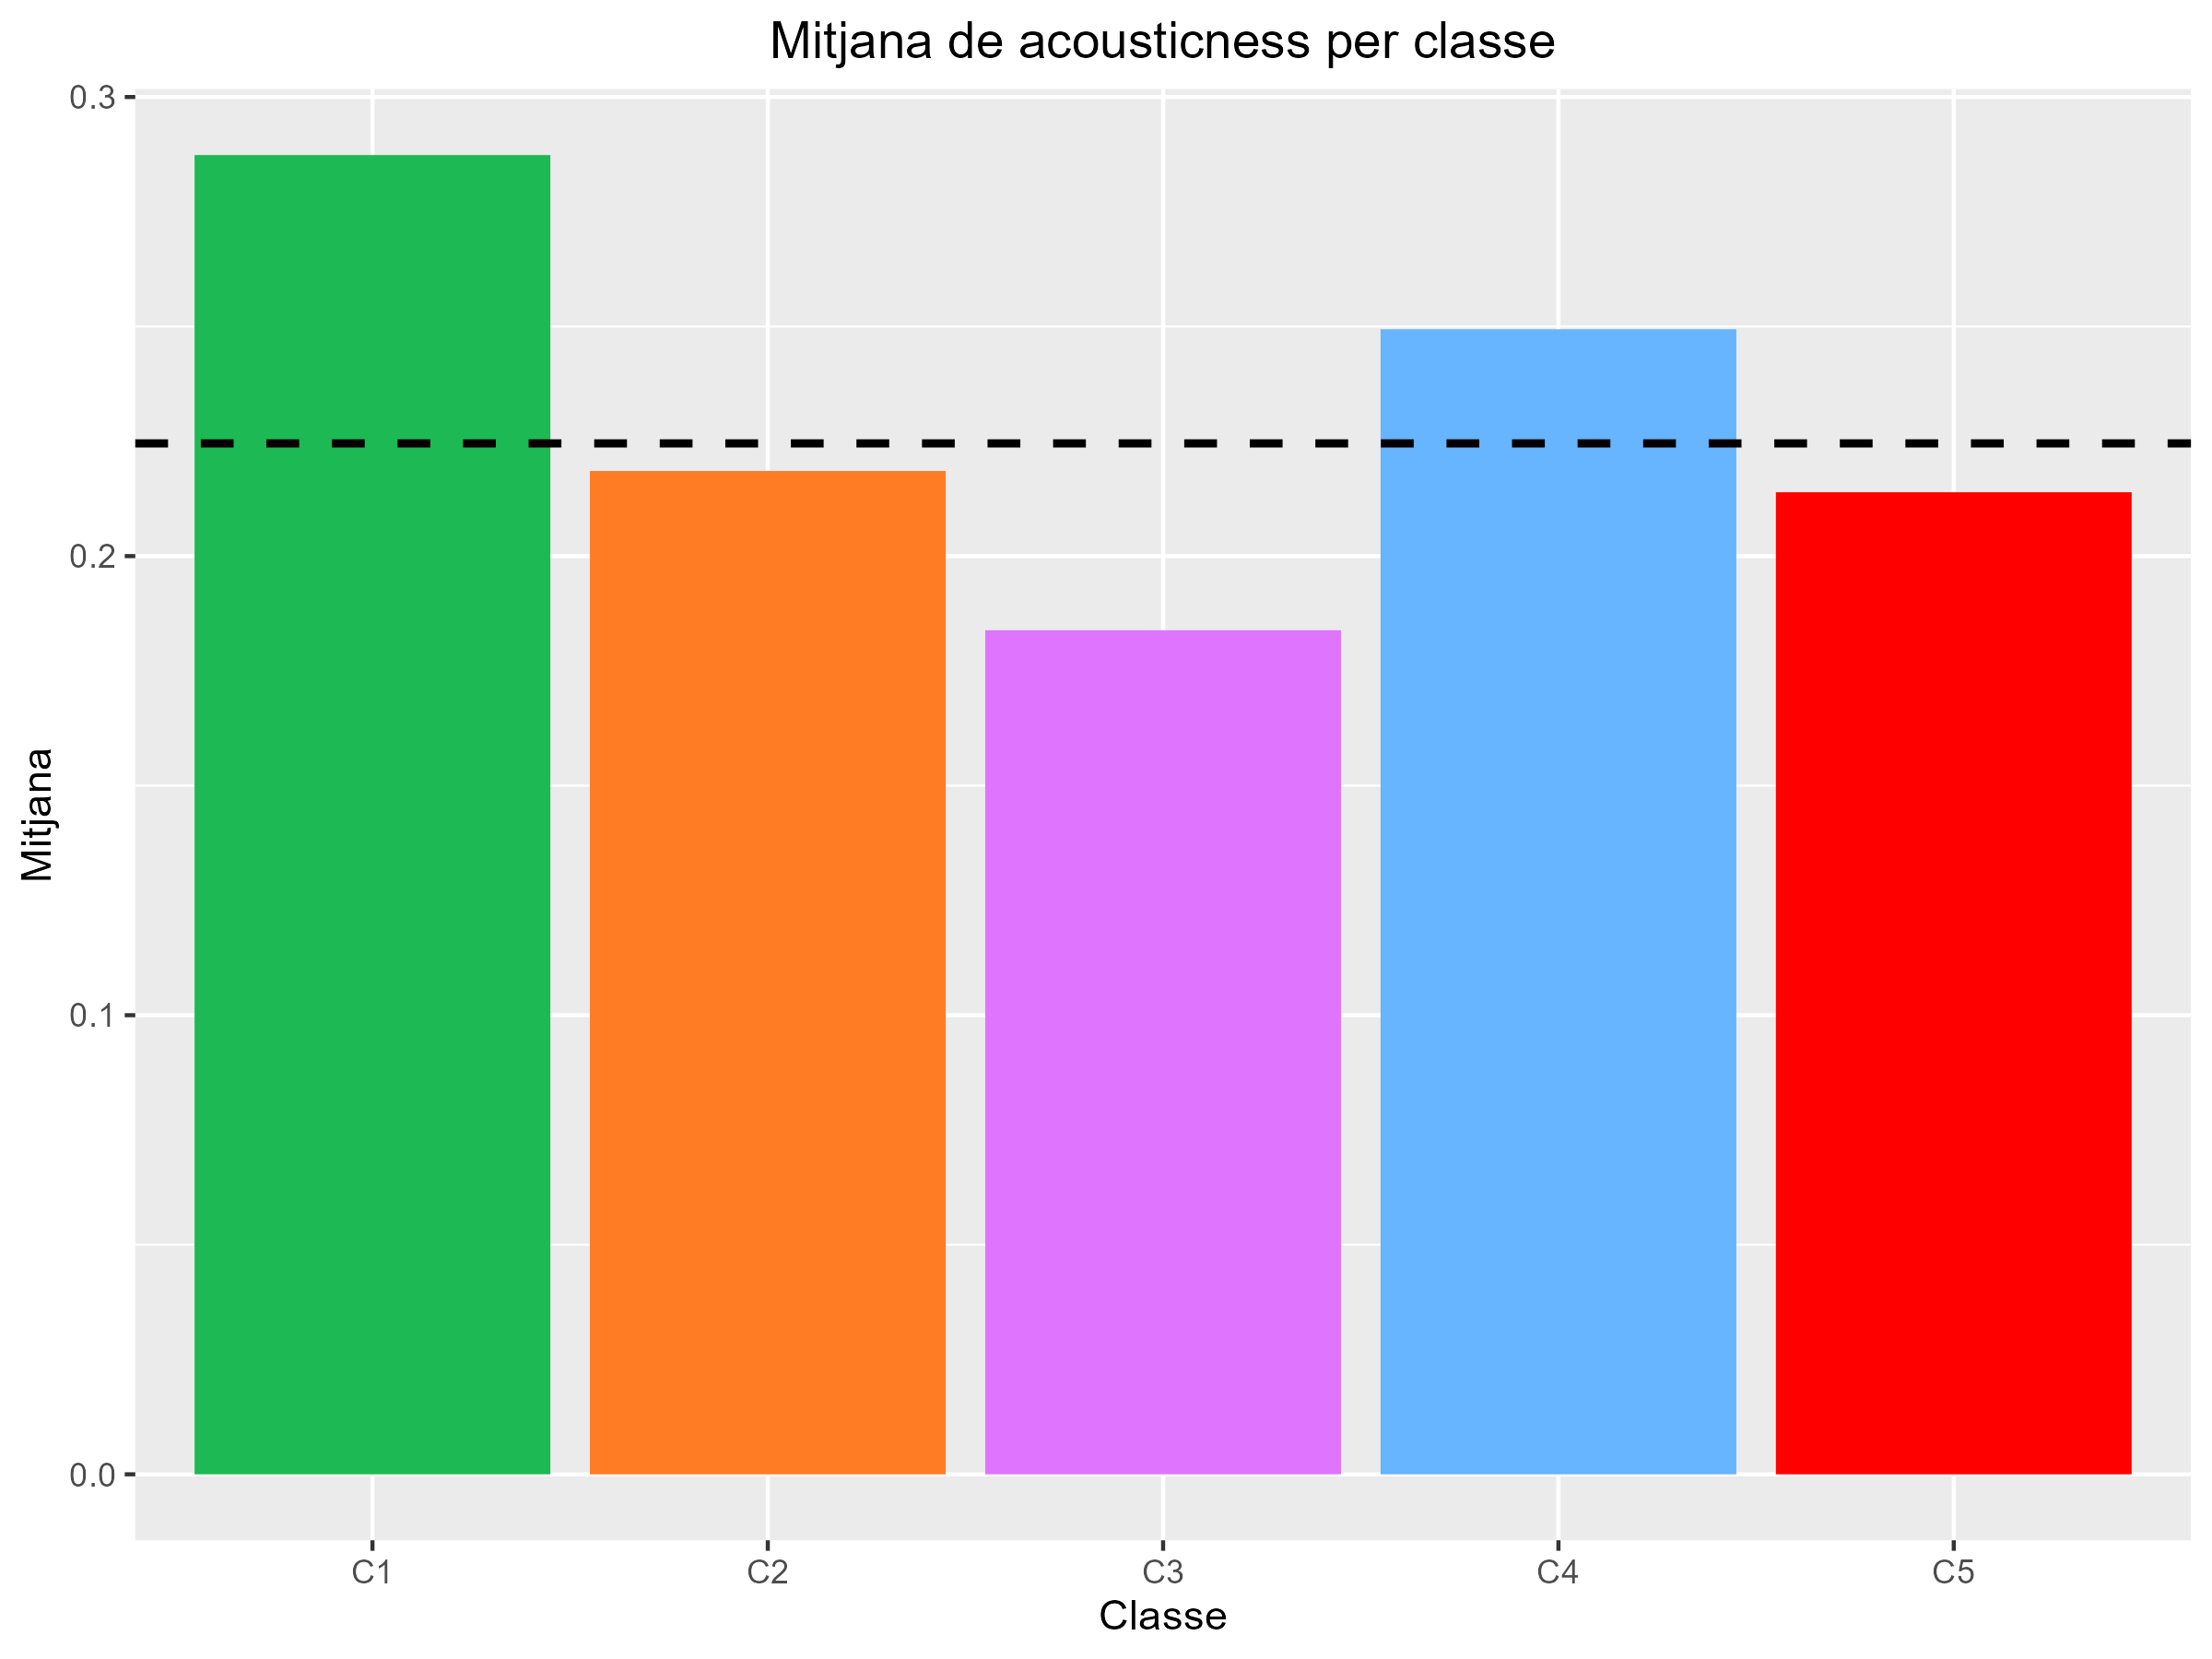
\includegraphics[width=0.95\linewidth]{Images/5_Profiling/numeriques/Num_BarPlot_acousticness.png}
        \caption{Barplot amb les mitjanes \\ d'acousticness per clúster}
        \label{fig:Num_BarPlot_acousticness}
    \end{minipage}%
    \begin{minipage}{.49\textwidth}
        \centering
        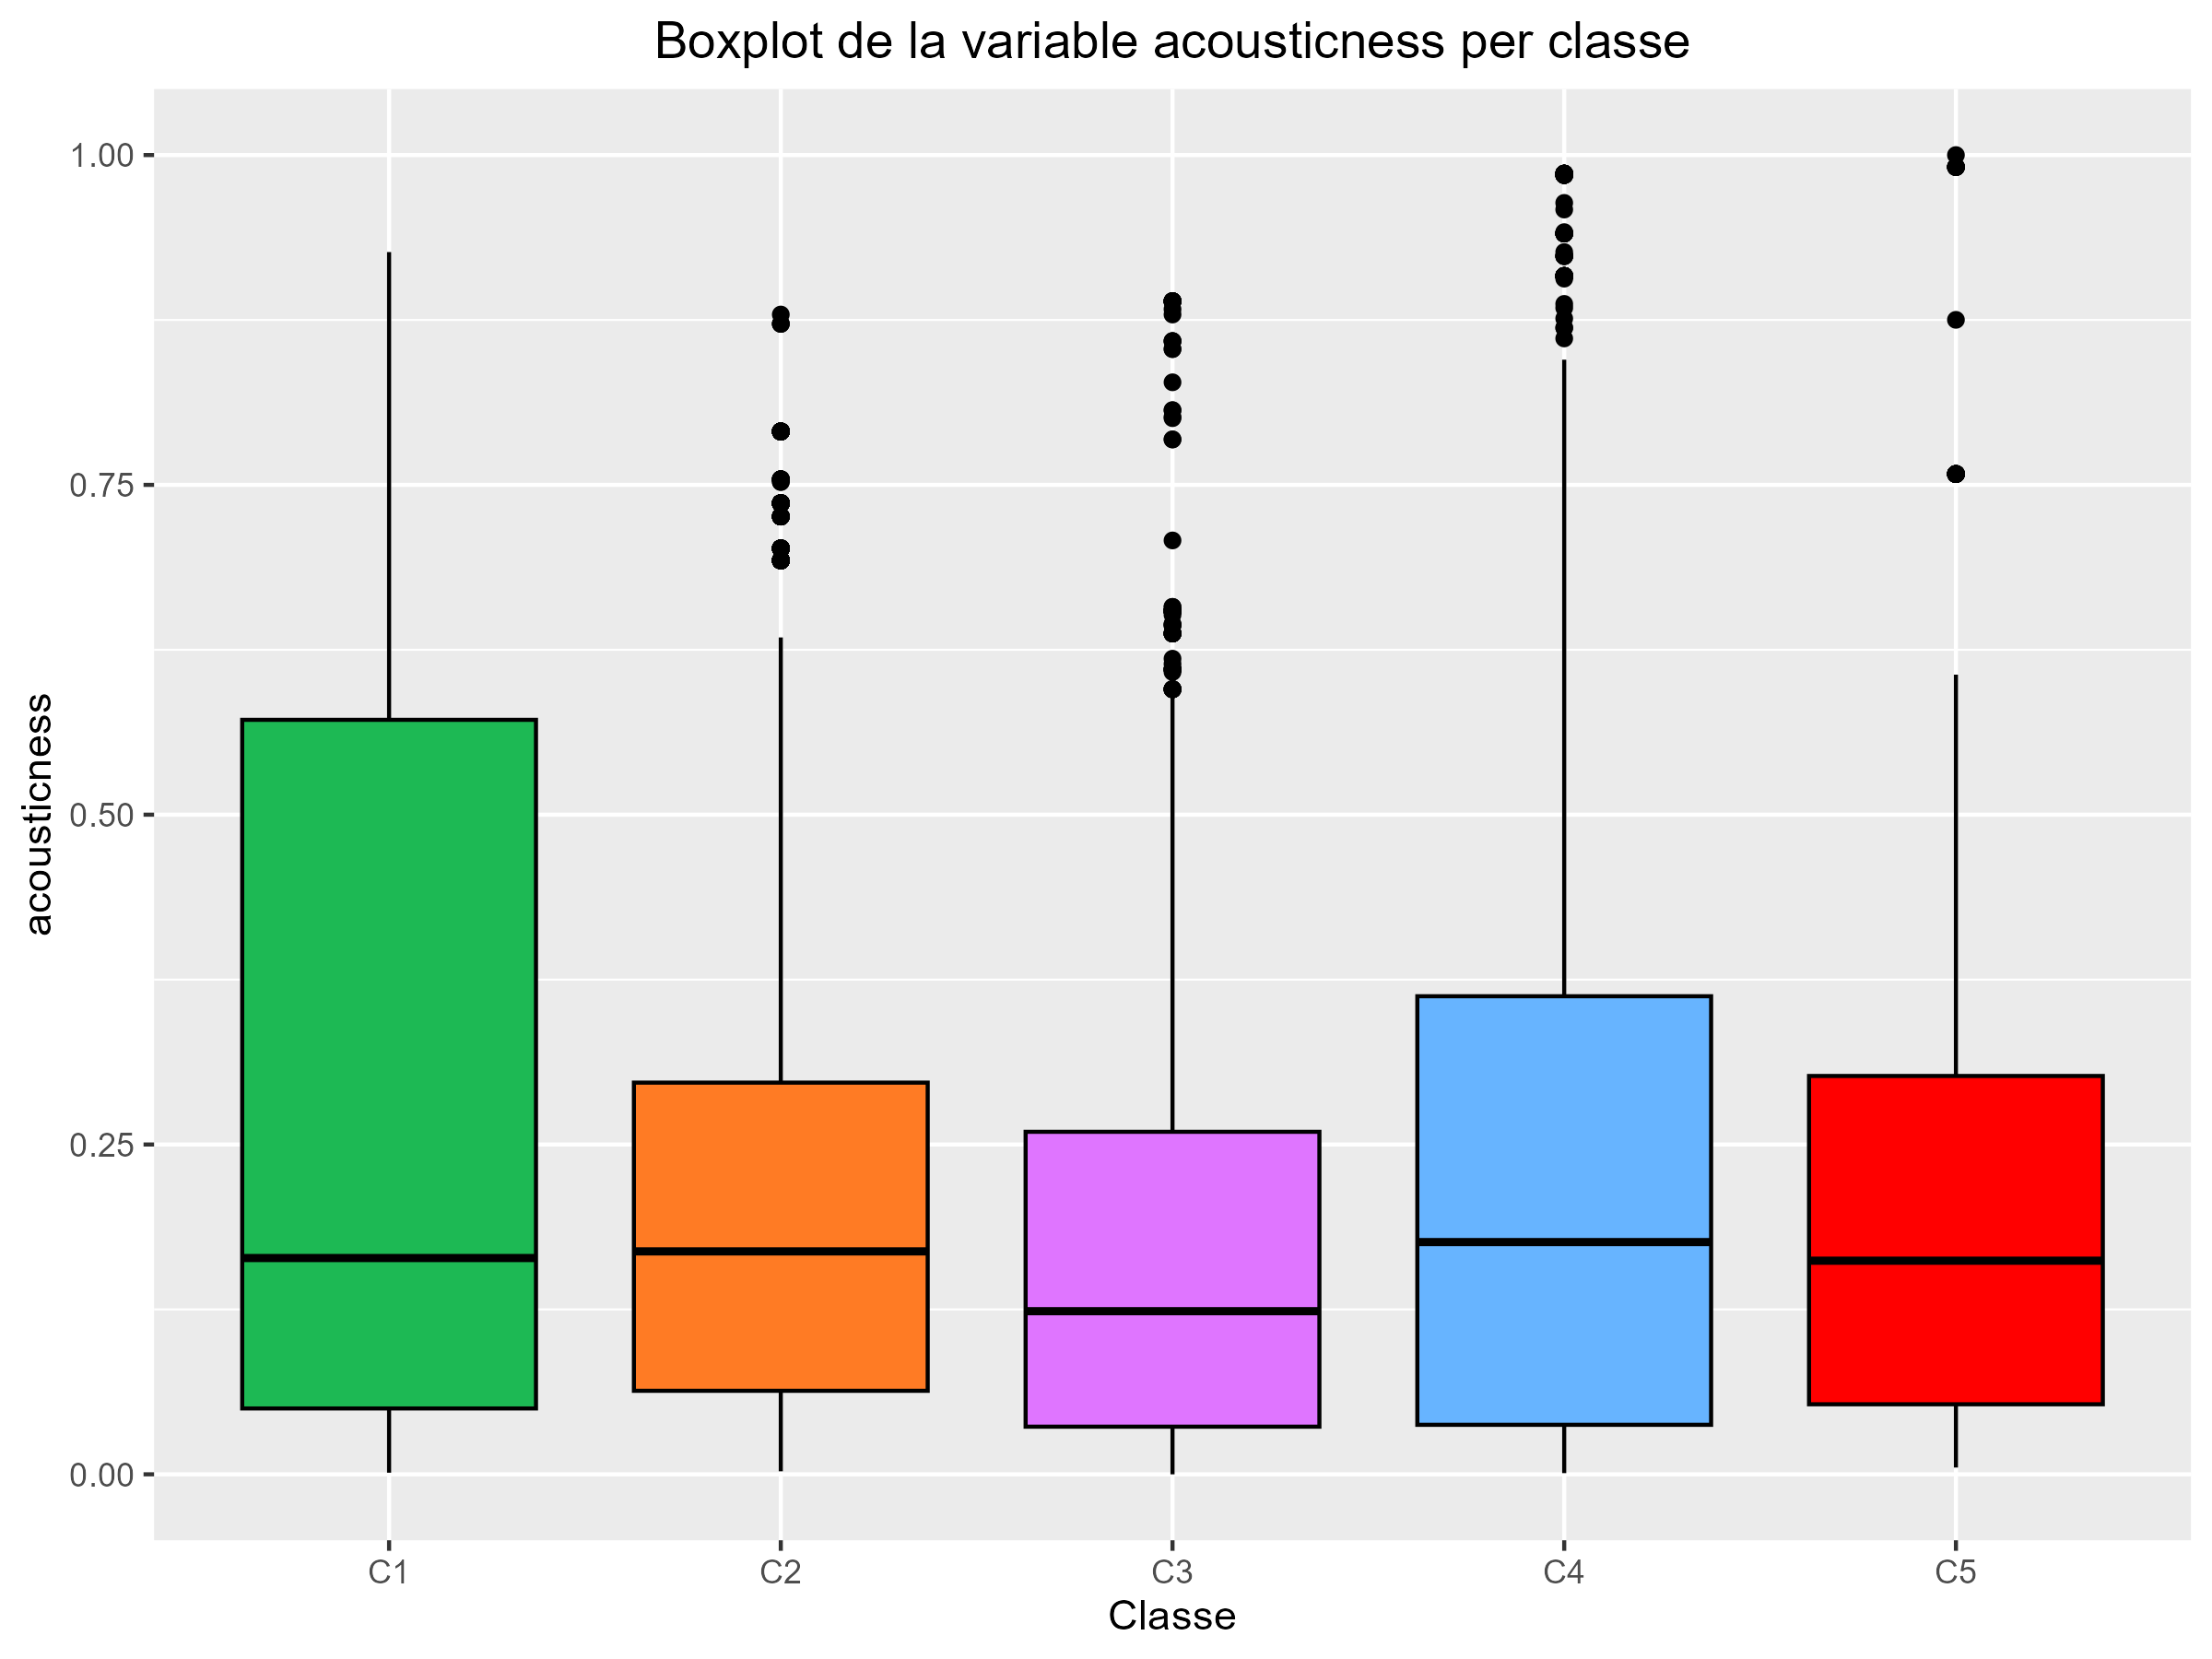
\includegraphics[width=0.95\linewidth]{Images/5_Profiling/numeriques/Num_BoxPlot_acousticness.png}
        \caption{Boxplots d'acousticness per clúster}
        \label{fig:Num_BoxPlot_acousticness}
    \end{minipage}%
\end{figure}

La primera variable en la que ens fixem és l'acousticness. Veiem que la mitjana del primer clúster és molt més alta que la dels altres. Això ens indica que a la primera classe és on hi ha les cançons més aviat acústiques. Les classes dos i cinc tenen la mitjana pràcticament igual que la mitjana total, cosa que vol dir que no els hi afecta lo acústica que és una cançó. Finalment la classe 3 és la que té la mitjana més baixa de la total volent dir que allà hi ha cançons menys acústiques. 

\begin{figure}[H]
\centering
    \begin{minipage}{.49\textwidth}
        \centering
        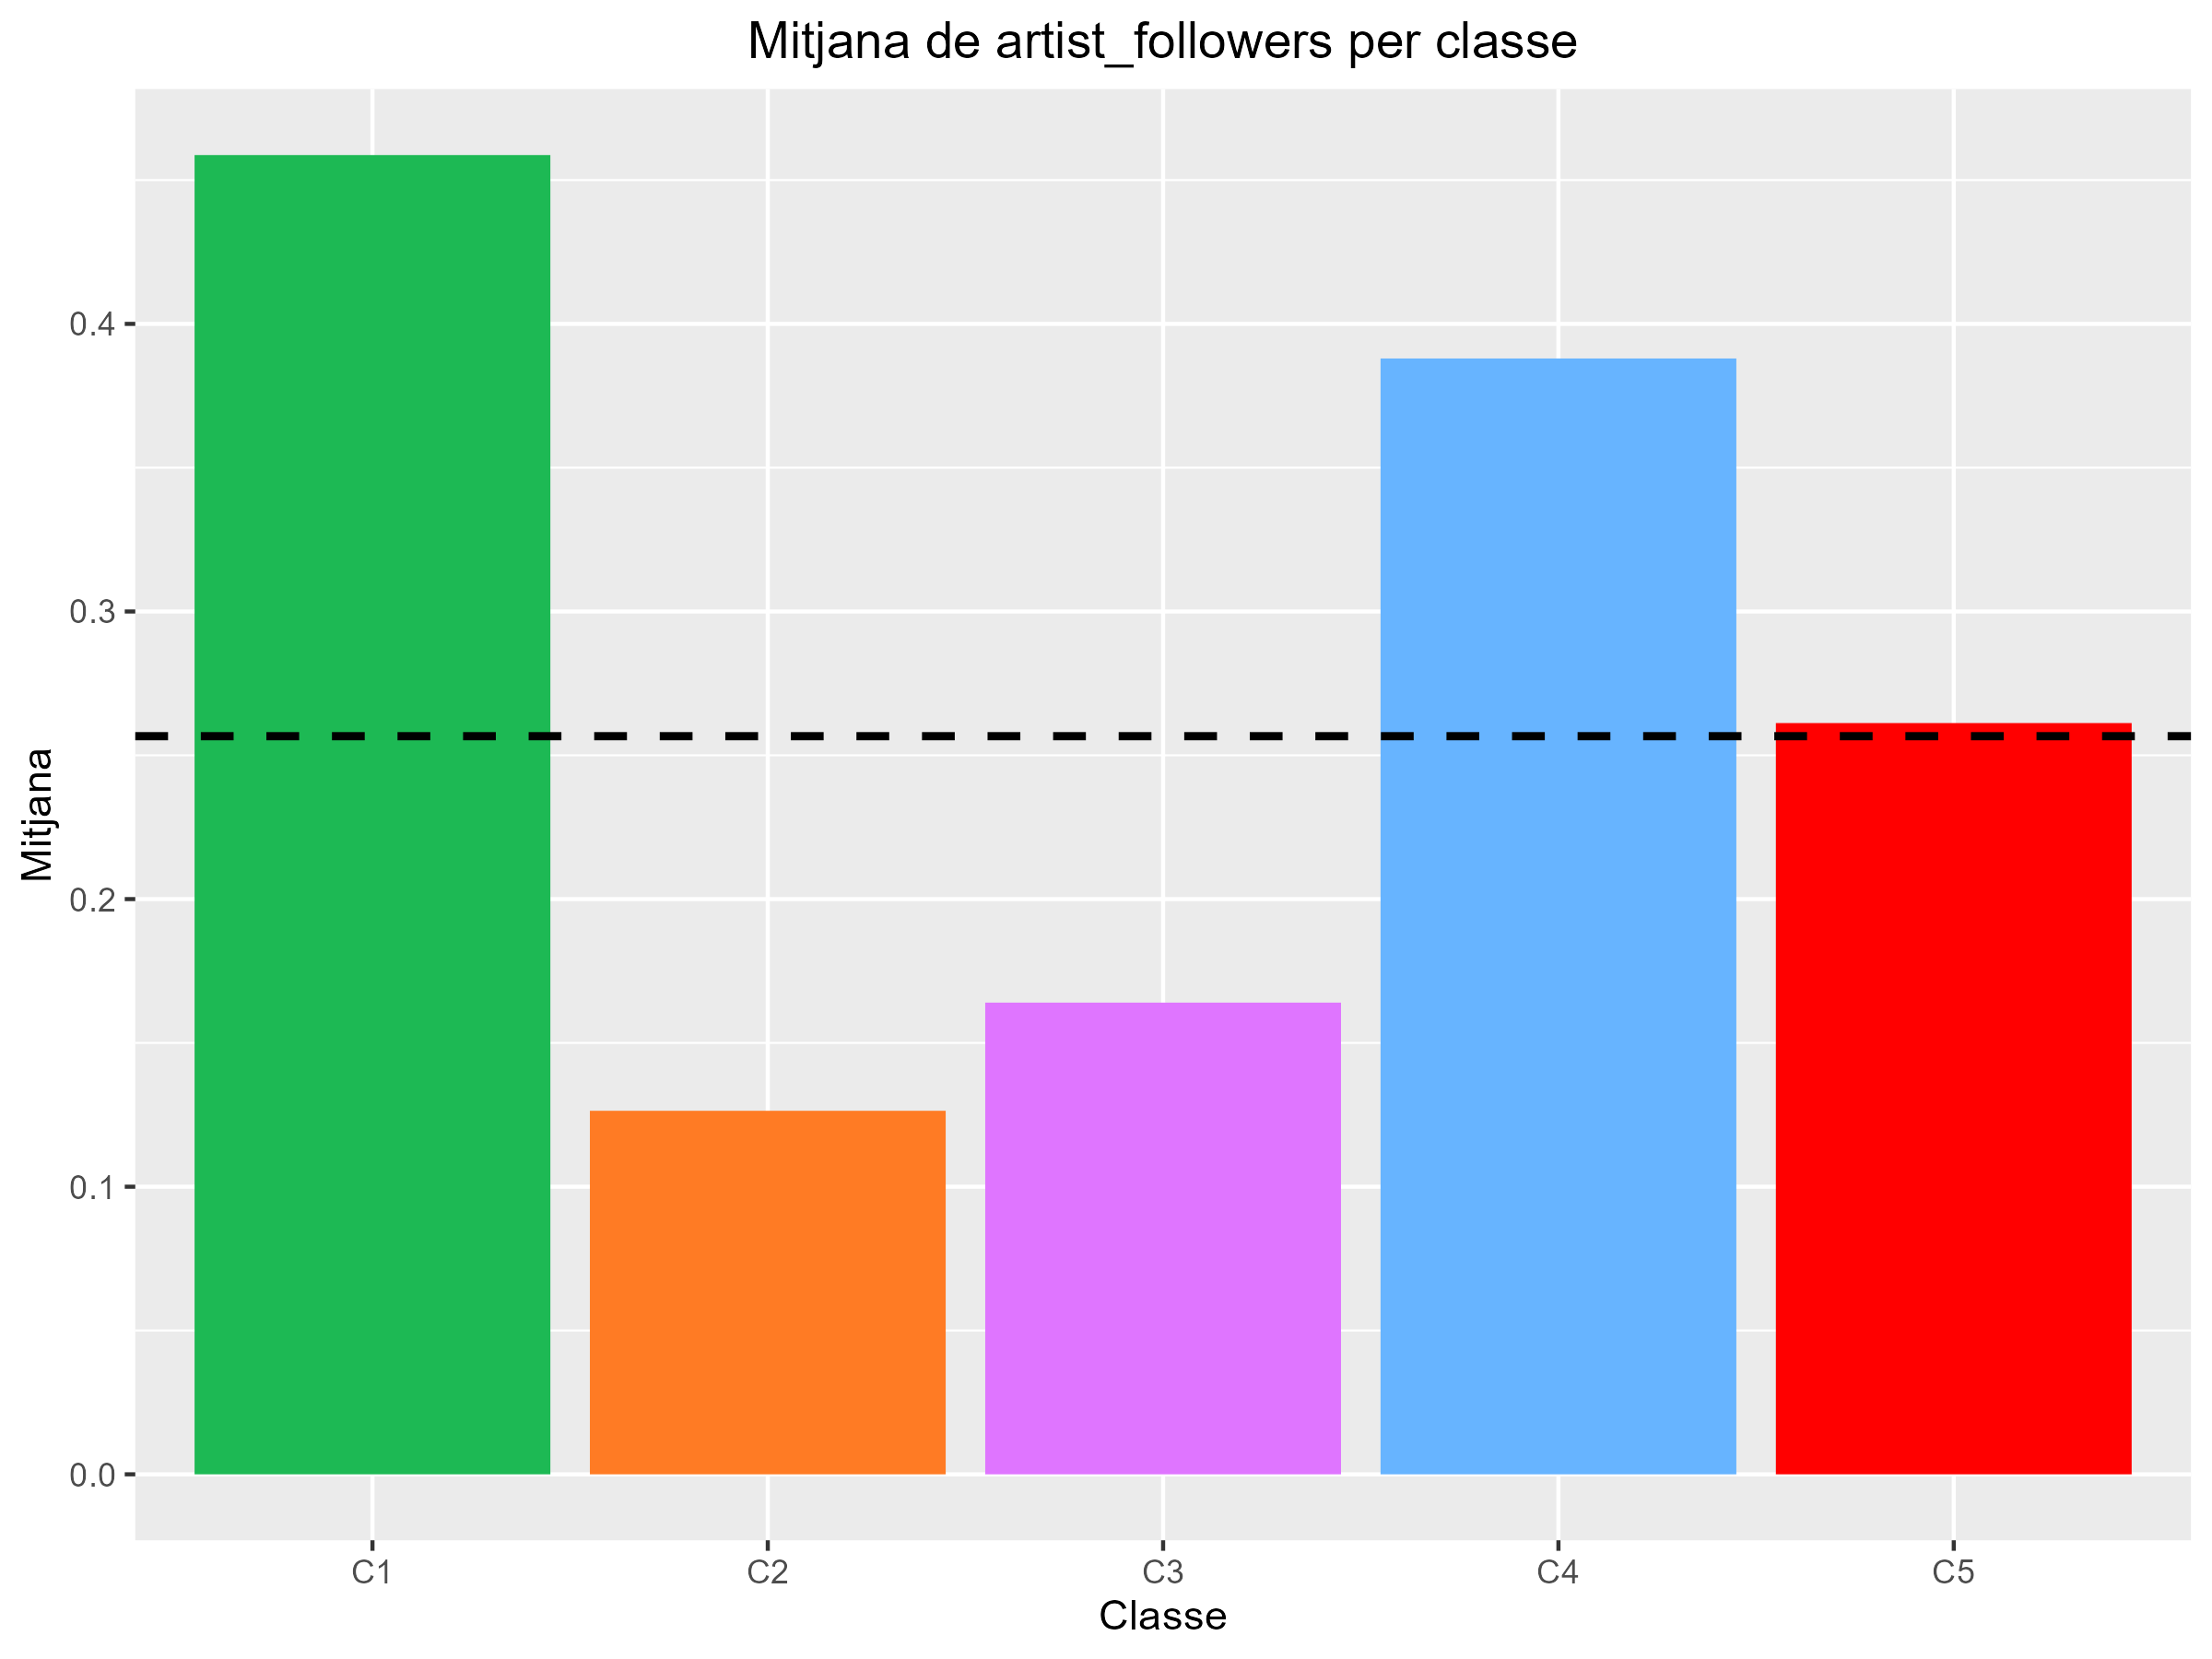
\includegraphics[width=0.95\linewidth]{Images/5_Profiling/numeriques/Num_BarPlot_artist_followers.png}
        \caption{Barplot amb les mitjanes \\ d'artist\_followers per clúster}
        \label{fig:Num_BarPlot_artist_followers}
    \end{minipage}%
    \begin{minipage}{.49\textwidth}
        \centering
        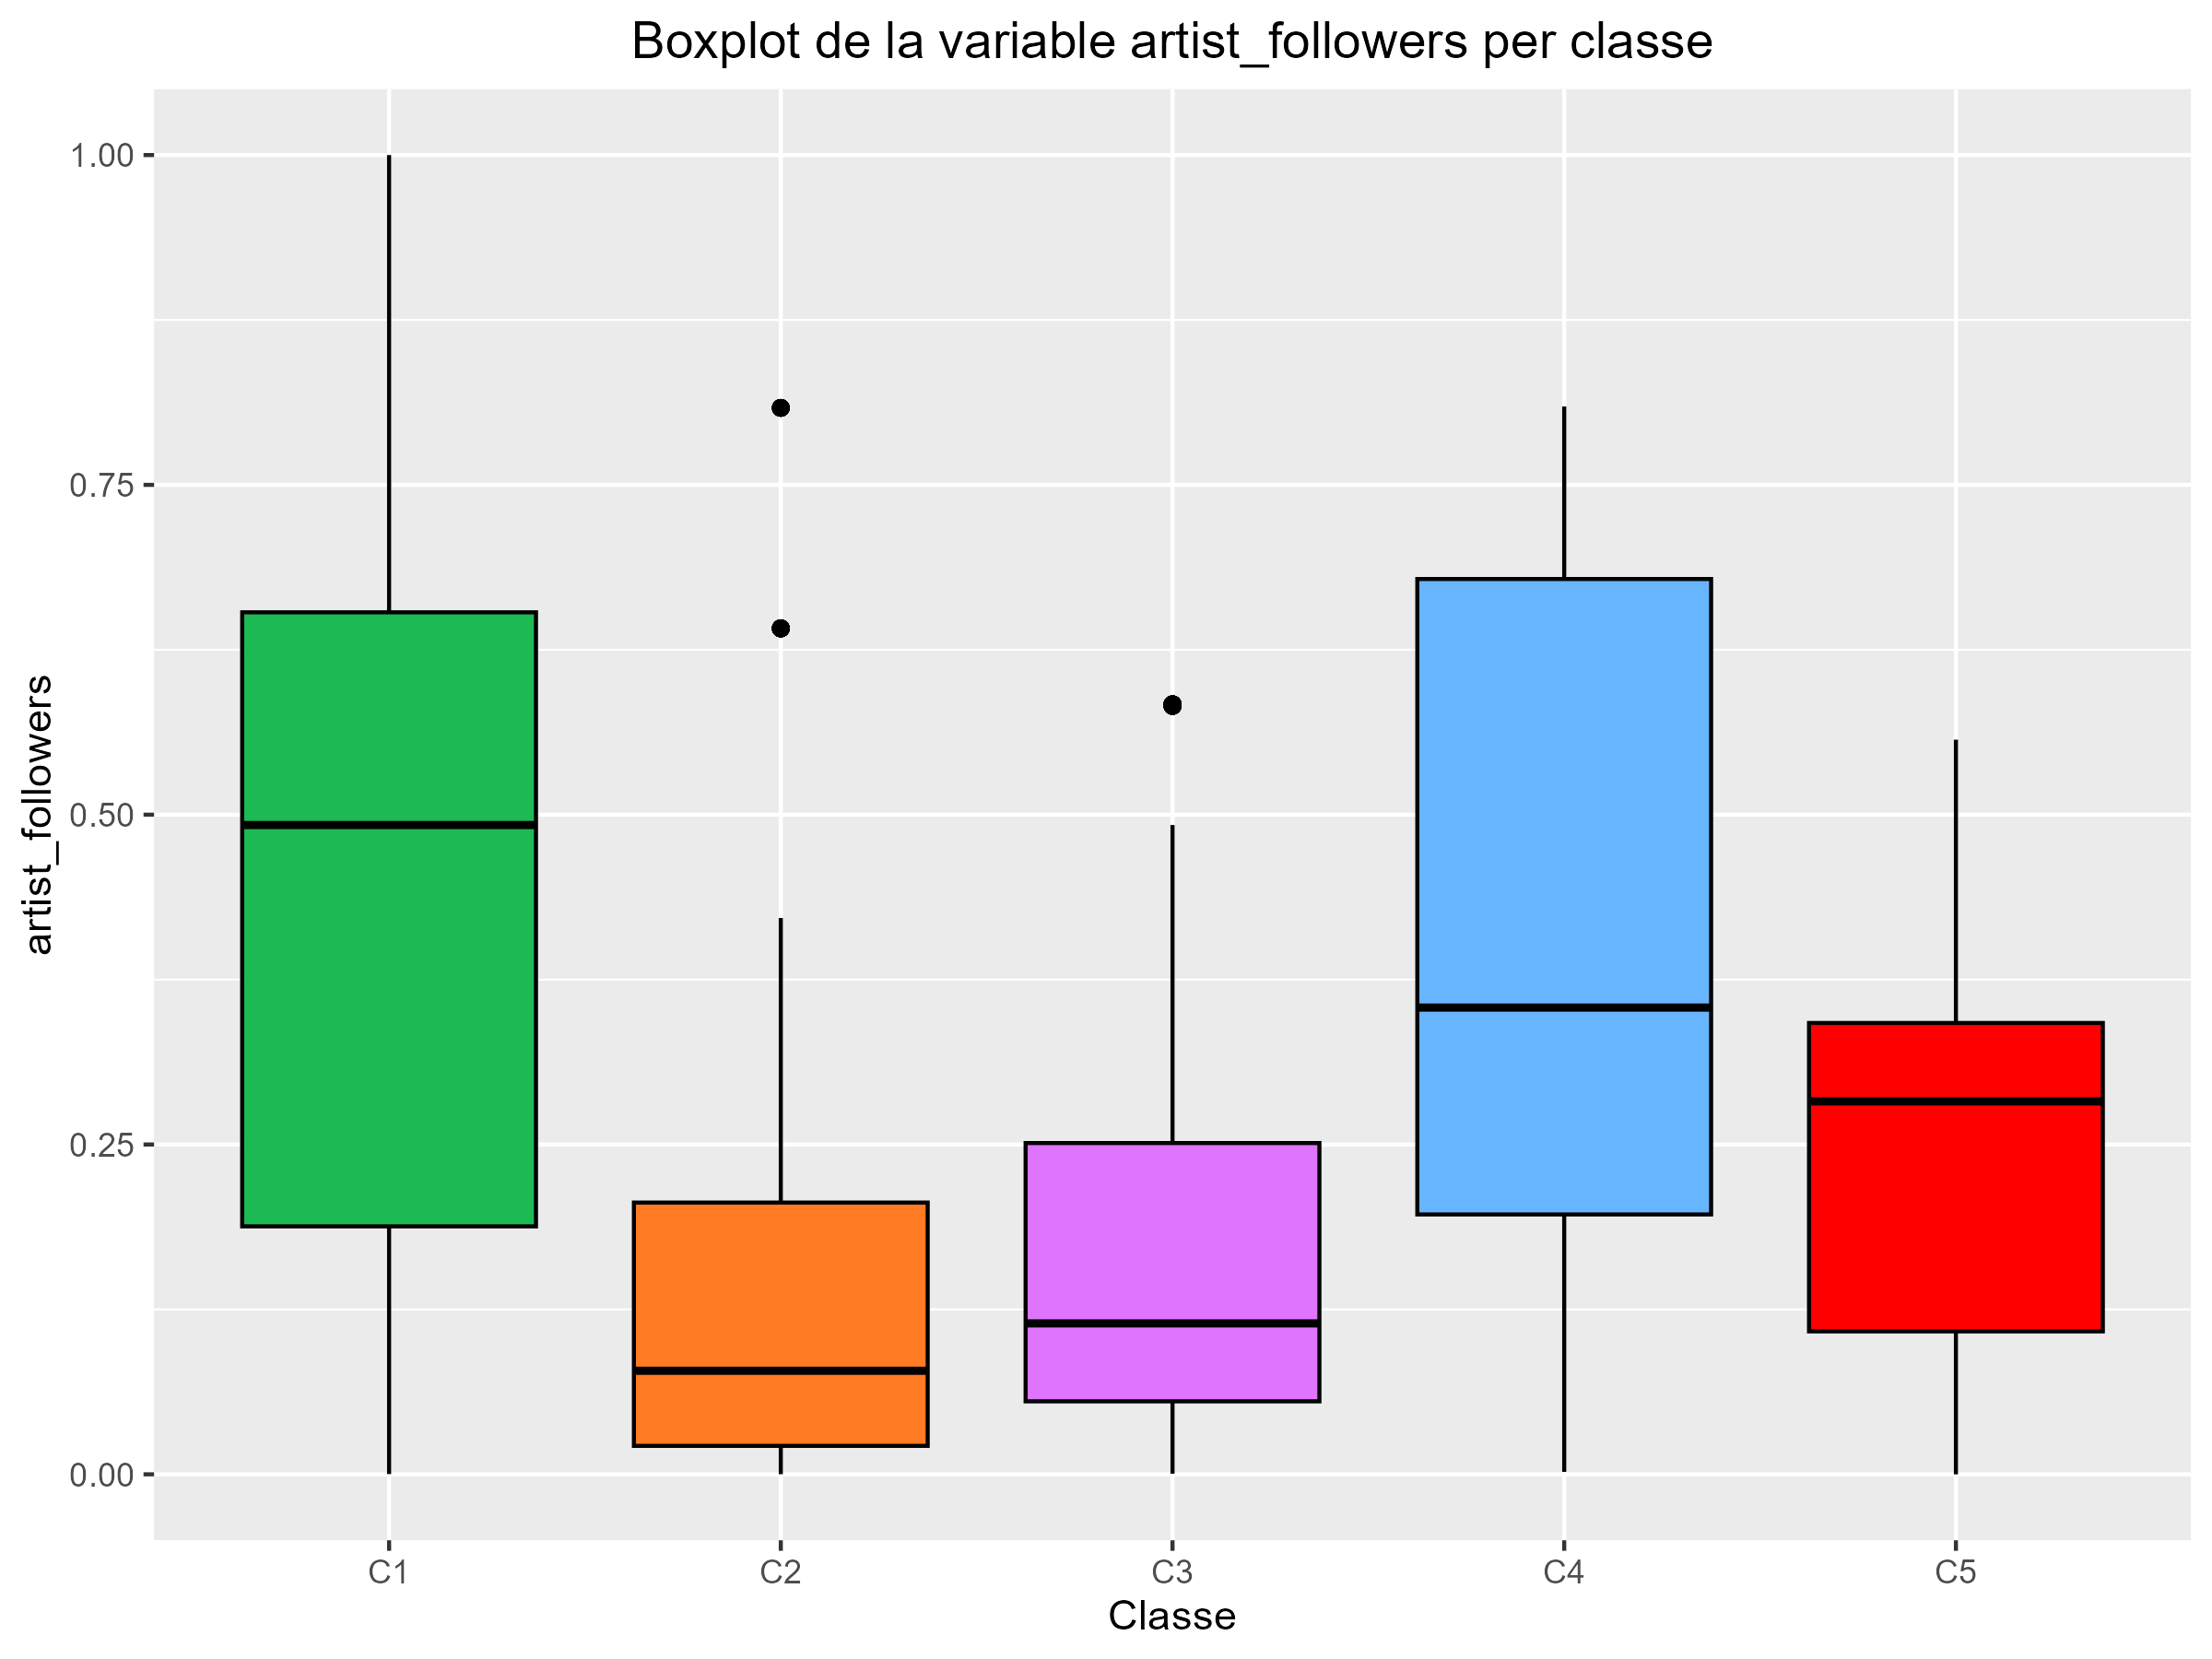
\includegraphics[width=0.95\linewidth]{Images/5_Profiling/numeriques/Num_BoxPlot_artist_followers.png}
        \caption{Boxplots d'artist\_followers per clúster}
        \label{fig:Num_BoxPlot_artist_followers}
    \end{minipage}%
\end{figure}

També es veuen diferències molt significatives entre les mitjanes d'artist\_followers. Veiem que, amb molta diferència, la classe u és on hi ha els artistes amb més followers. La classe quatre també té artistes amb molts seguidors, i hi ha molta diferència amb els clústers 2 i 3 que tenen la mitjana molt baixa i per tant tenen molts menys seguidors. Finalment, la classe 5 té la mateixa mitjana que la total indicant que no li afecten els seguidors de l'artista. 

\begin{figure}[H]
\centering
    \begin{minipage}{.49\textwidth}
        \centering
        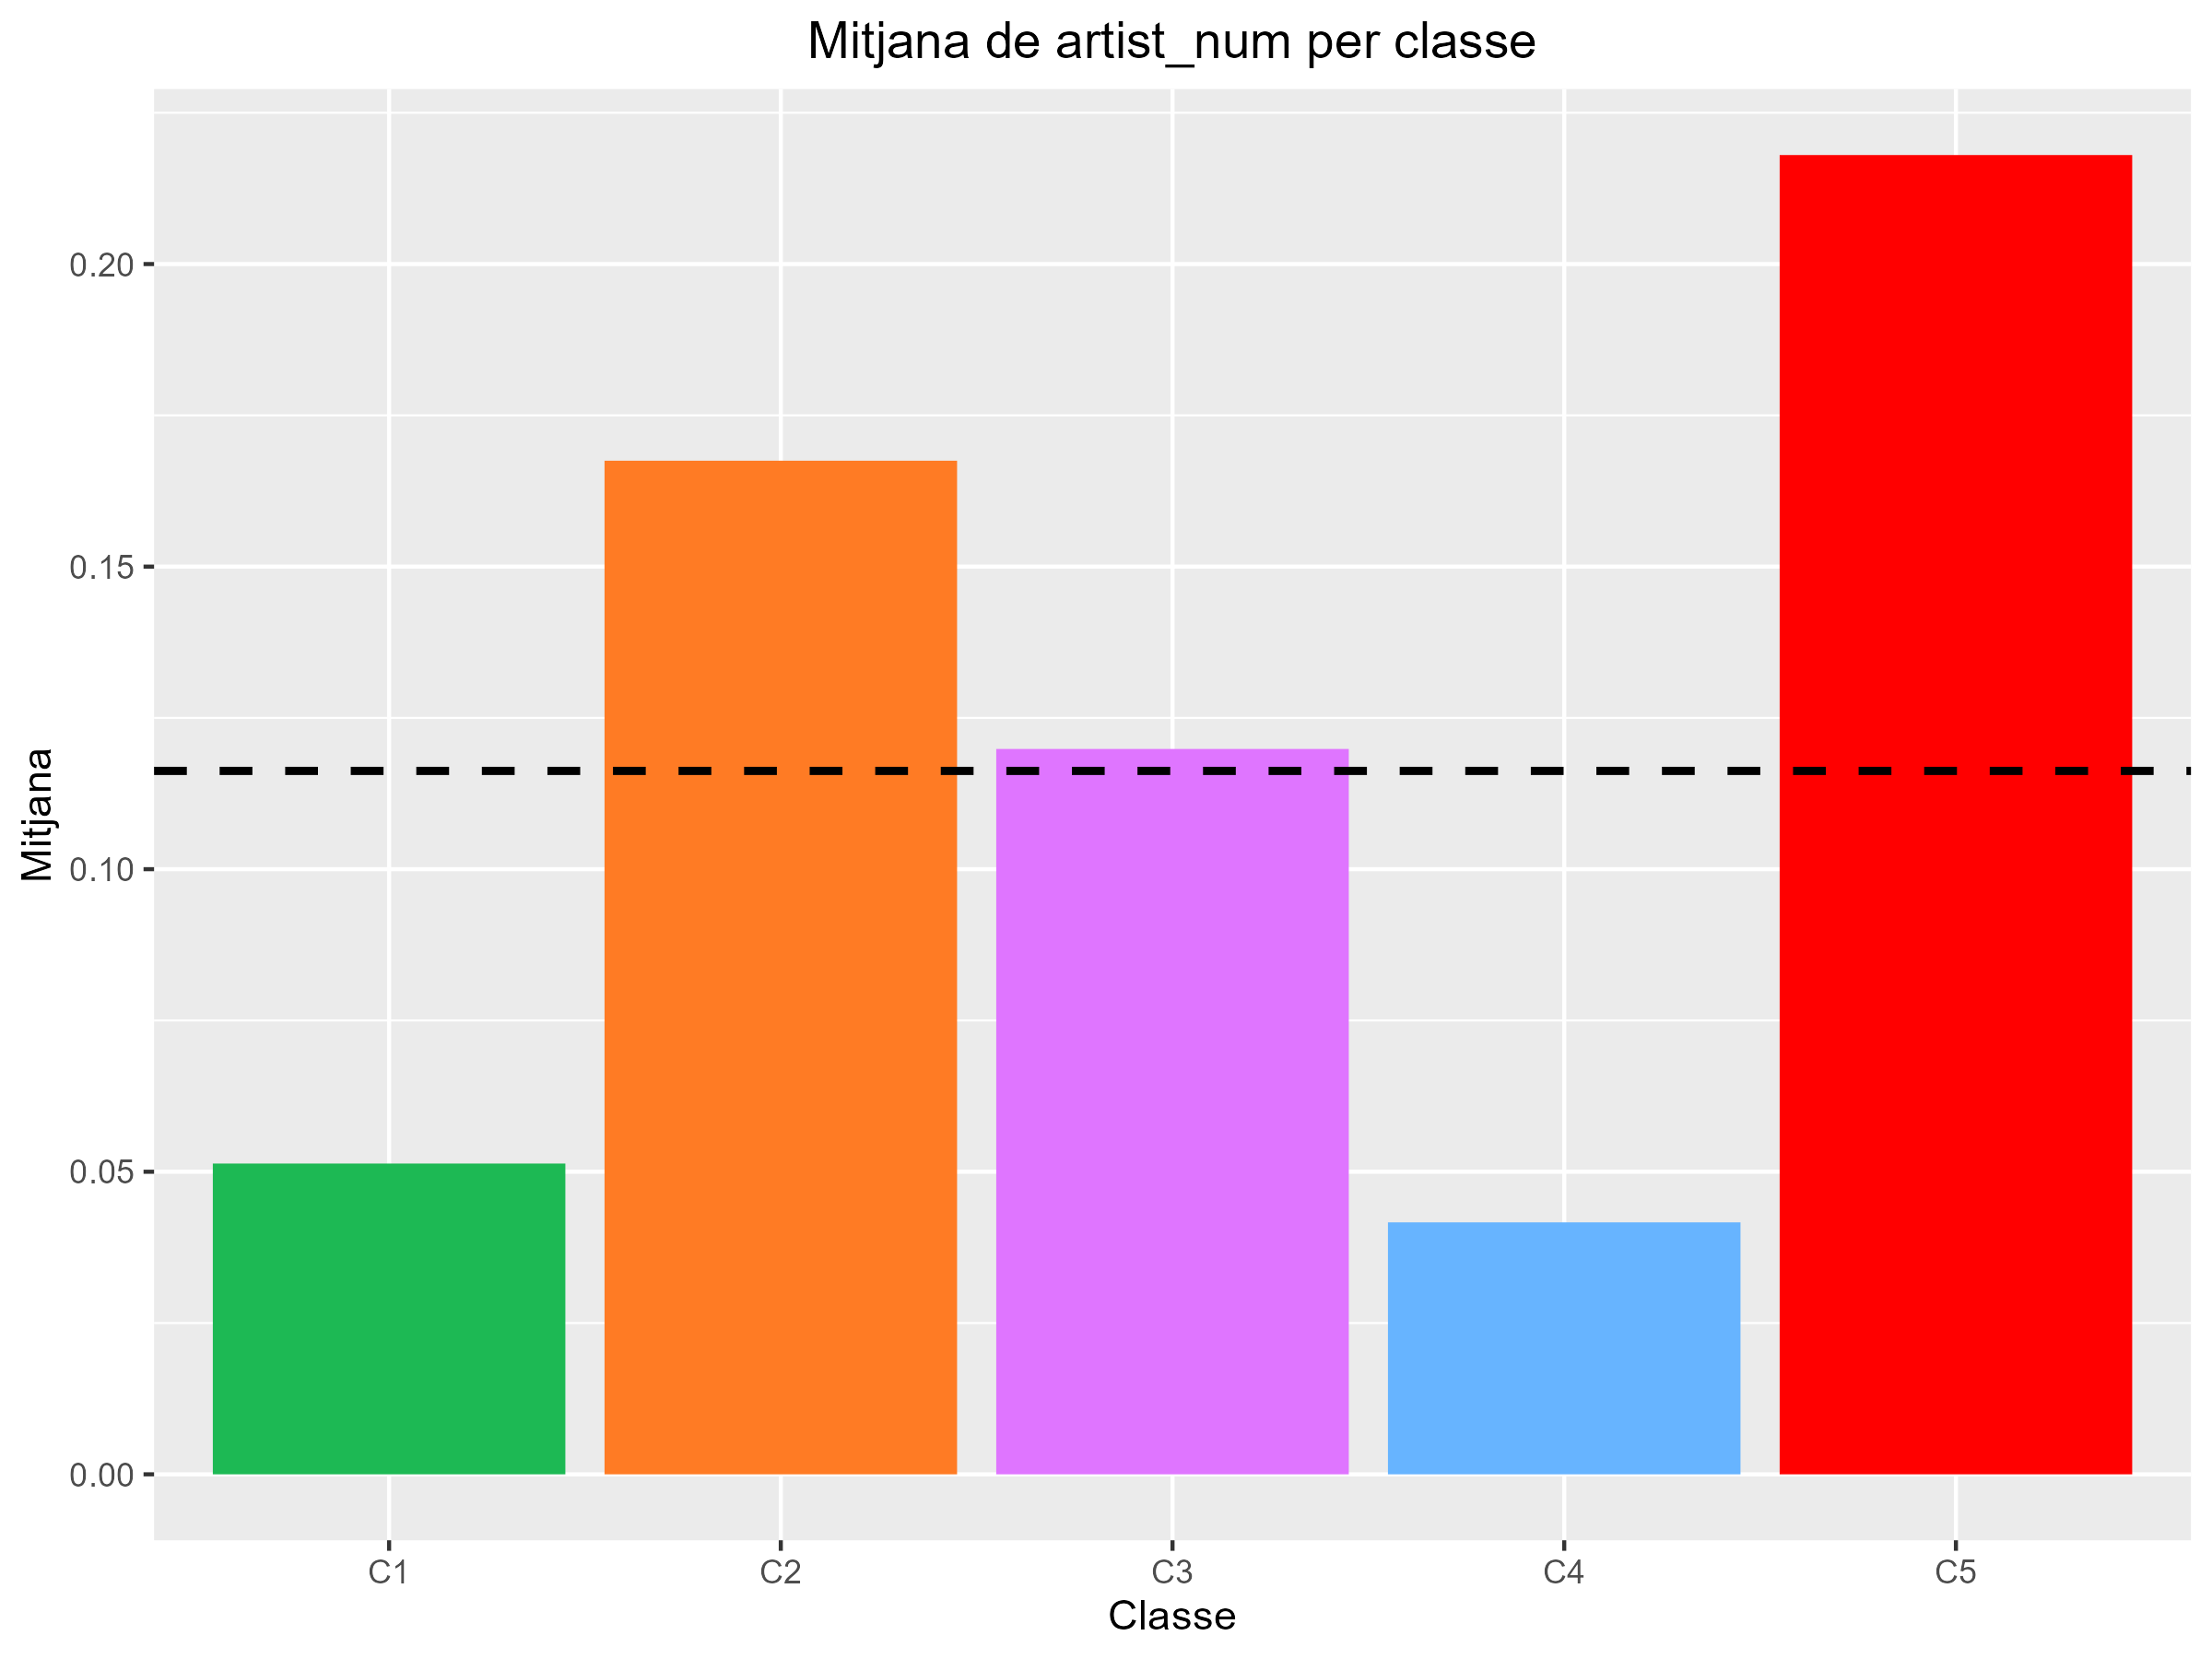
\includegraphics[width=0.95\linewidth]{Images/5_Profiling/numeriques/Num_BarPlot_artist_num.png}
        \caption{Barplot amb les mitjanes \\ d'artist\_num per clúster}
        \label{fig:Num_BarPlot_artist_num}
    \end{minipage}%
    \begin{minipage}{.49\textwidth}
        \centering
        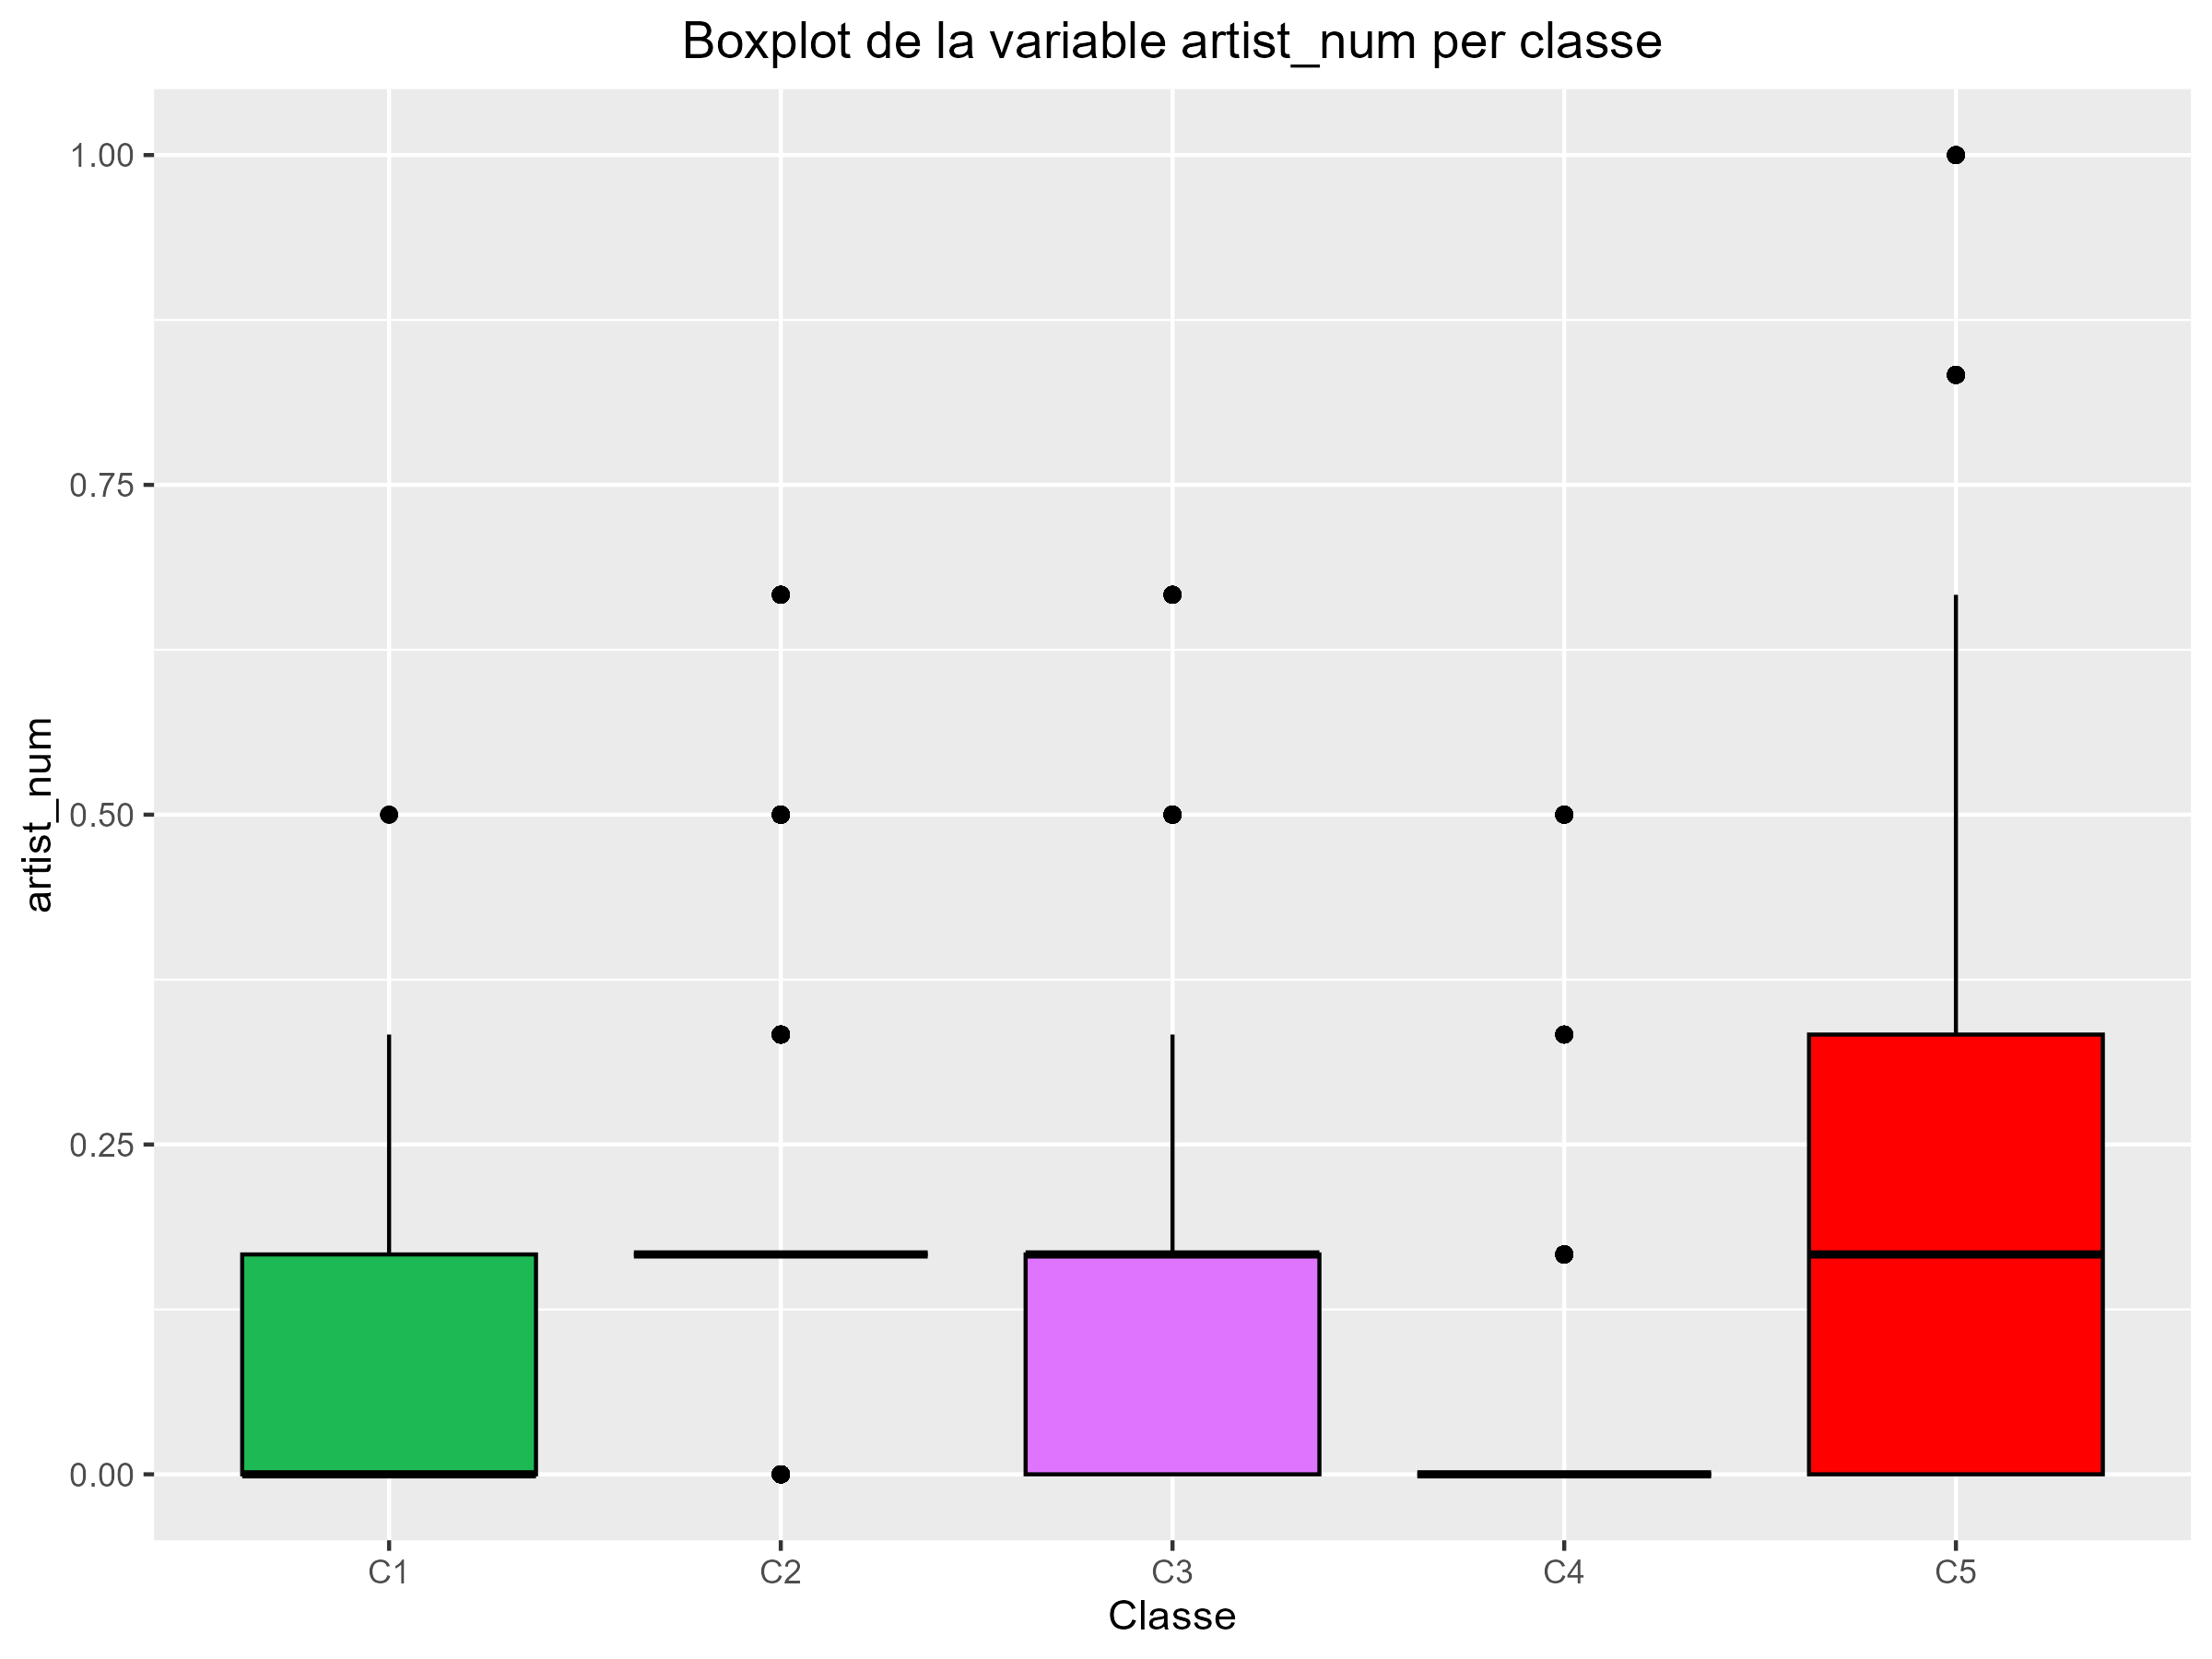
\includegraphics[width=0.95\linewidth]{Images/5_Profiling/numeriques/Num_BoxPlot_artist_num.png}
        \caption{Boxplots d'artist\_num per clúster}
        \label{fig:Num_BoxPlot_artist_num}
    \end{minipage}%
\end{figure}
Artist\_num també veiem que és una variable que està afectant a la creació dels nostres clústers. Veiem que els clústers amb les mitjanes més baixes són el 1 i el 4, i això indica que tenen cançons que involucren a pocs artistes, o menys que la resta. En canvi, els clústers 2 i 5, sobretot el 5, tenen la mitjana molt més alta, i observant el boxplot trobem que allà és on estan les cançons que tenen, en general, molts més artistes colaborant. Hi ha una gran variabilitat en el nombre d'artistes que colaboren en aquest últim clúster. 

\begin{figure}[H]
\centering
    \begin{minipage}{.49\textwidth}
        \centering
        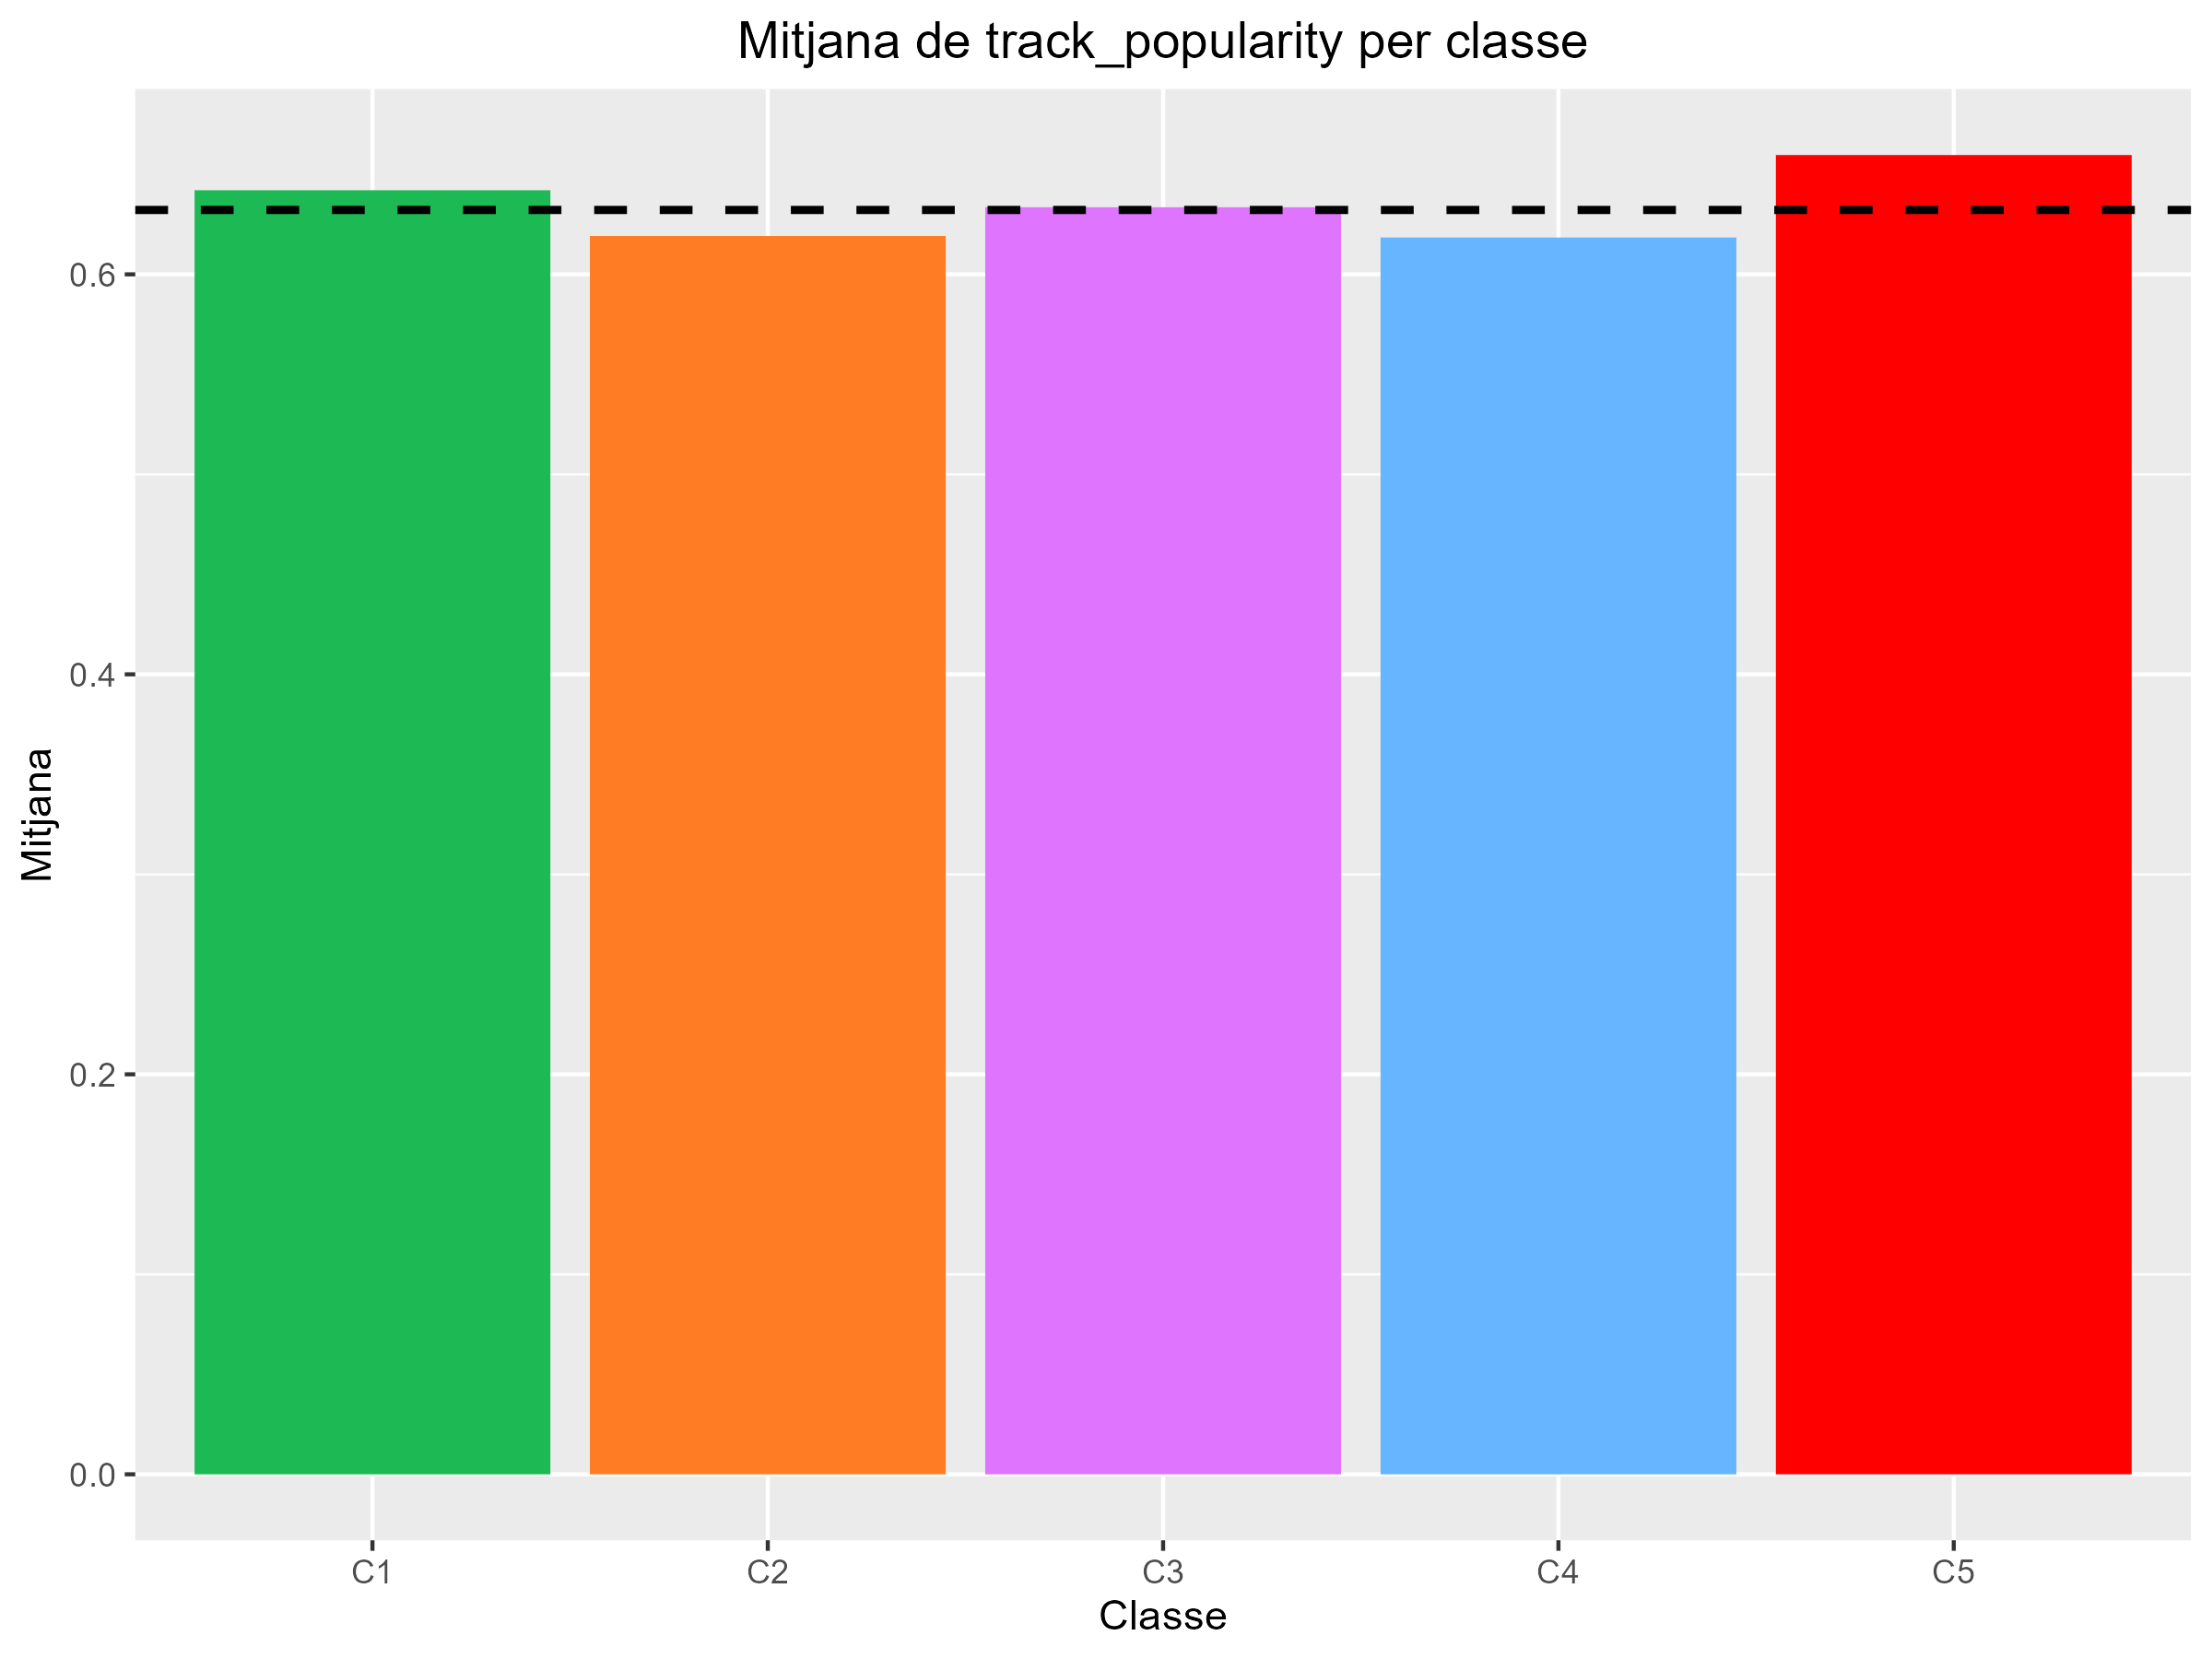
\includegraphics[width=0.95\linewidth]{Images/5_Profiling/numeriques/Num_BarPlot_track_popularity.png}
        \caption{Barplot amb les mitjanes \\ d'track\_popularity per clúster}
        \label{fig:Num_BarPlot_track_popularity}
    \end{minipage}%
    \begin{minipage}{.49\textwidth}
        \centering
        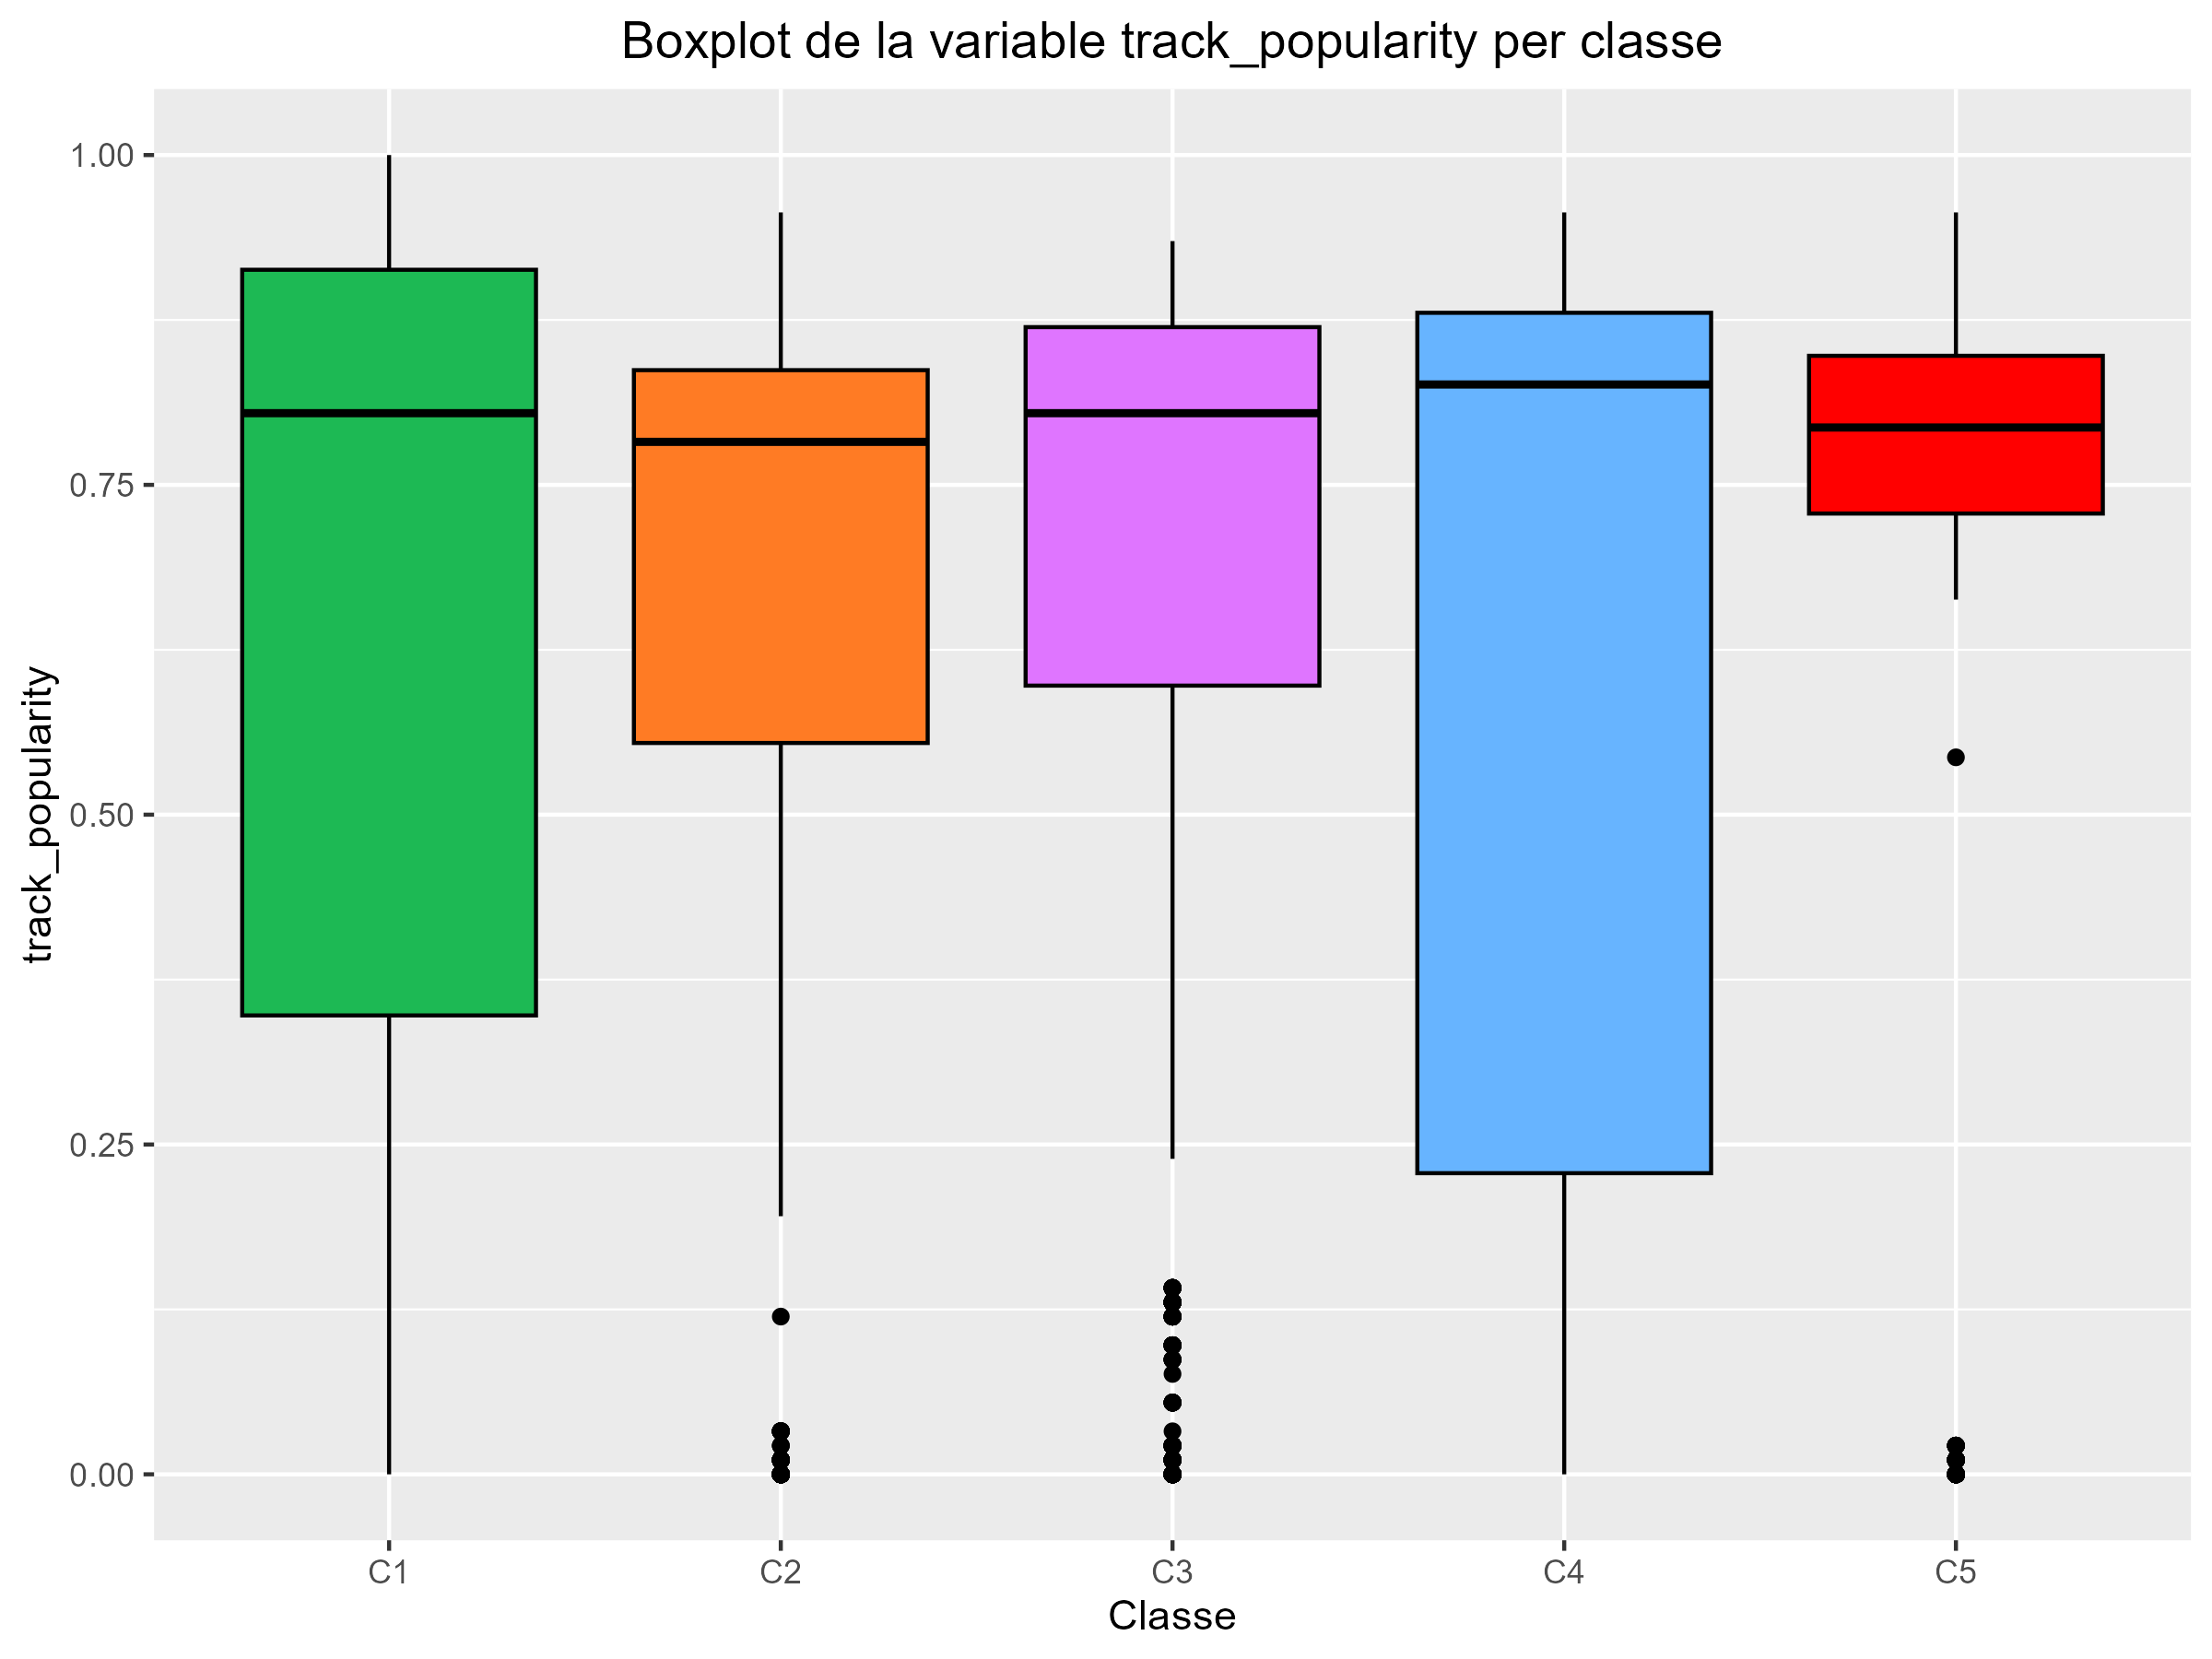
\includegraphics[width=0.95\linewidth]{Images/5_Profiling/numeriques/Num_BoxPlot_track_popularity.png}
        \caption{Boxplots d'track\_popularity per clúster}
        \label{fig:Num_BoxPlot_track_popularity}
    \end{minipage}%
\end{figure}

Una variable que ens ha sorprès molt és la variable track\_popularity, ja que l'any passat, els clústers es van dividir molt segons les popularitats de les cançons i dels albums i aquest any tots tenien mitjanes semblants. Tot i que al Barplot veiem que les mitjanes són totes extremadament semblants a la total, al Boxplot es descobreix que els clústers 1 i 4 tenen més variabilitat de les dades i allà és on es troben les cançons amb una mica menys de popularitat. 

\begin{figure}[H]
\centering
    \begin{minipage}{.49\textwidth}
        \centering
        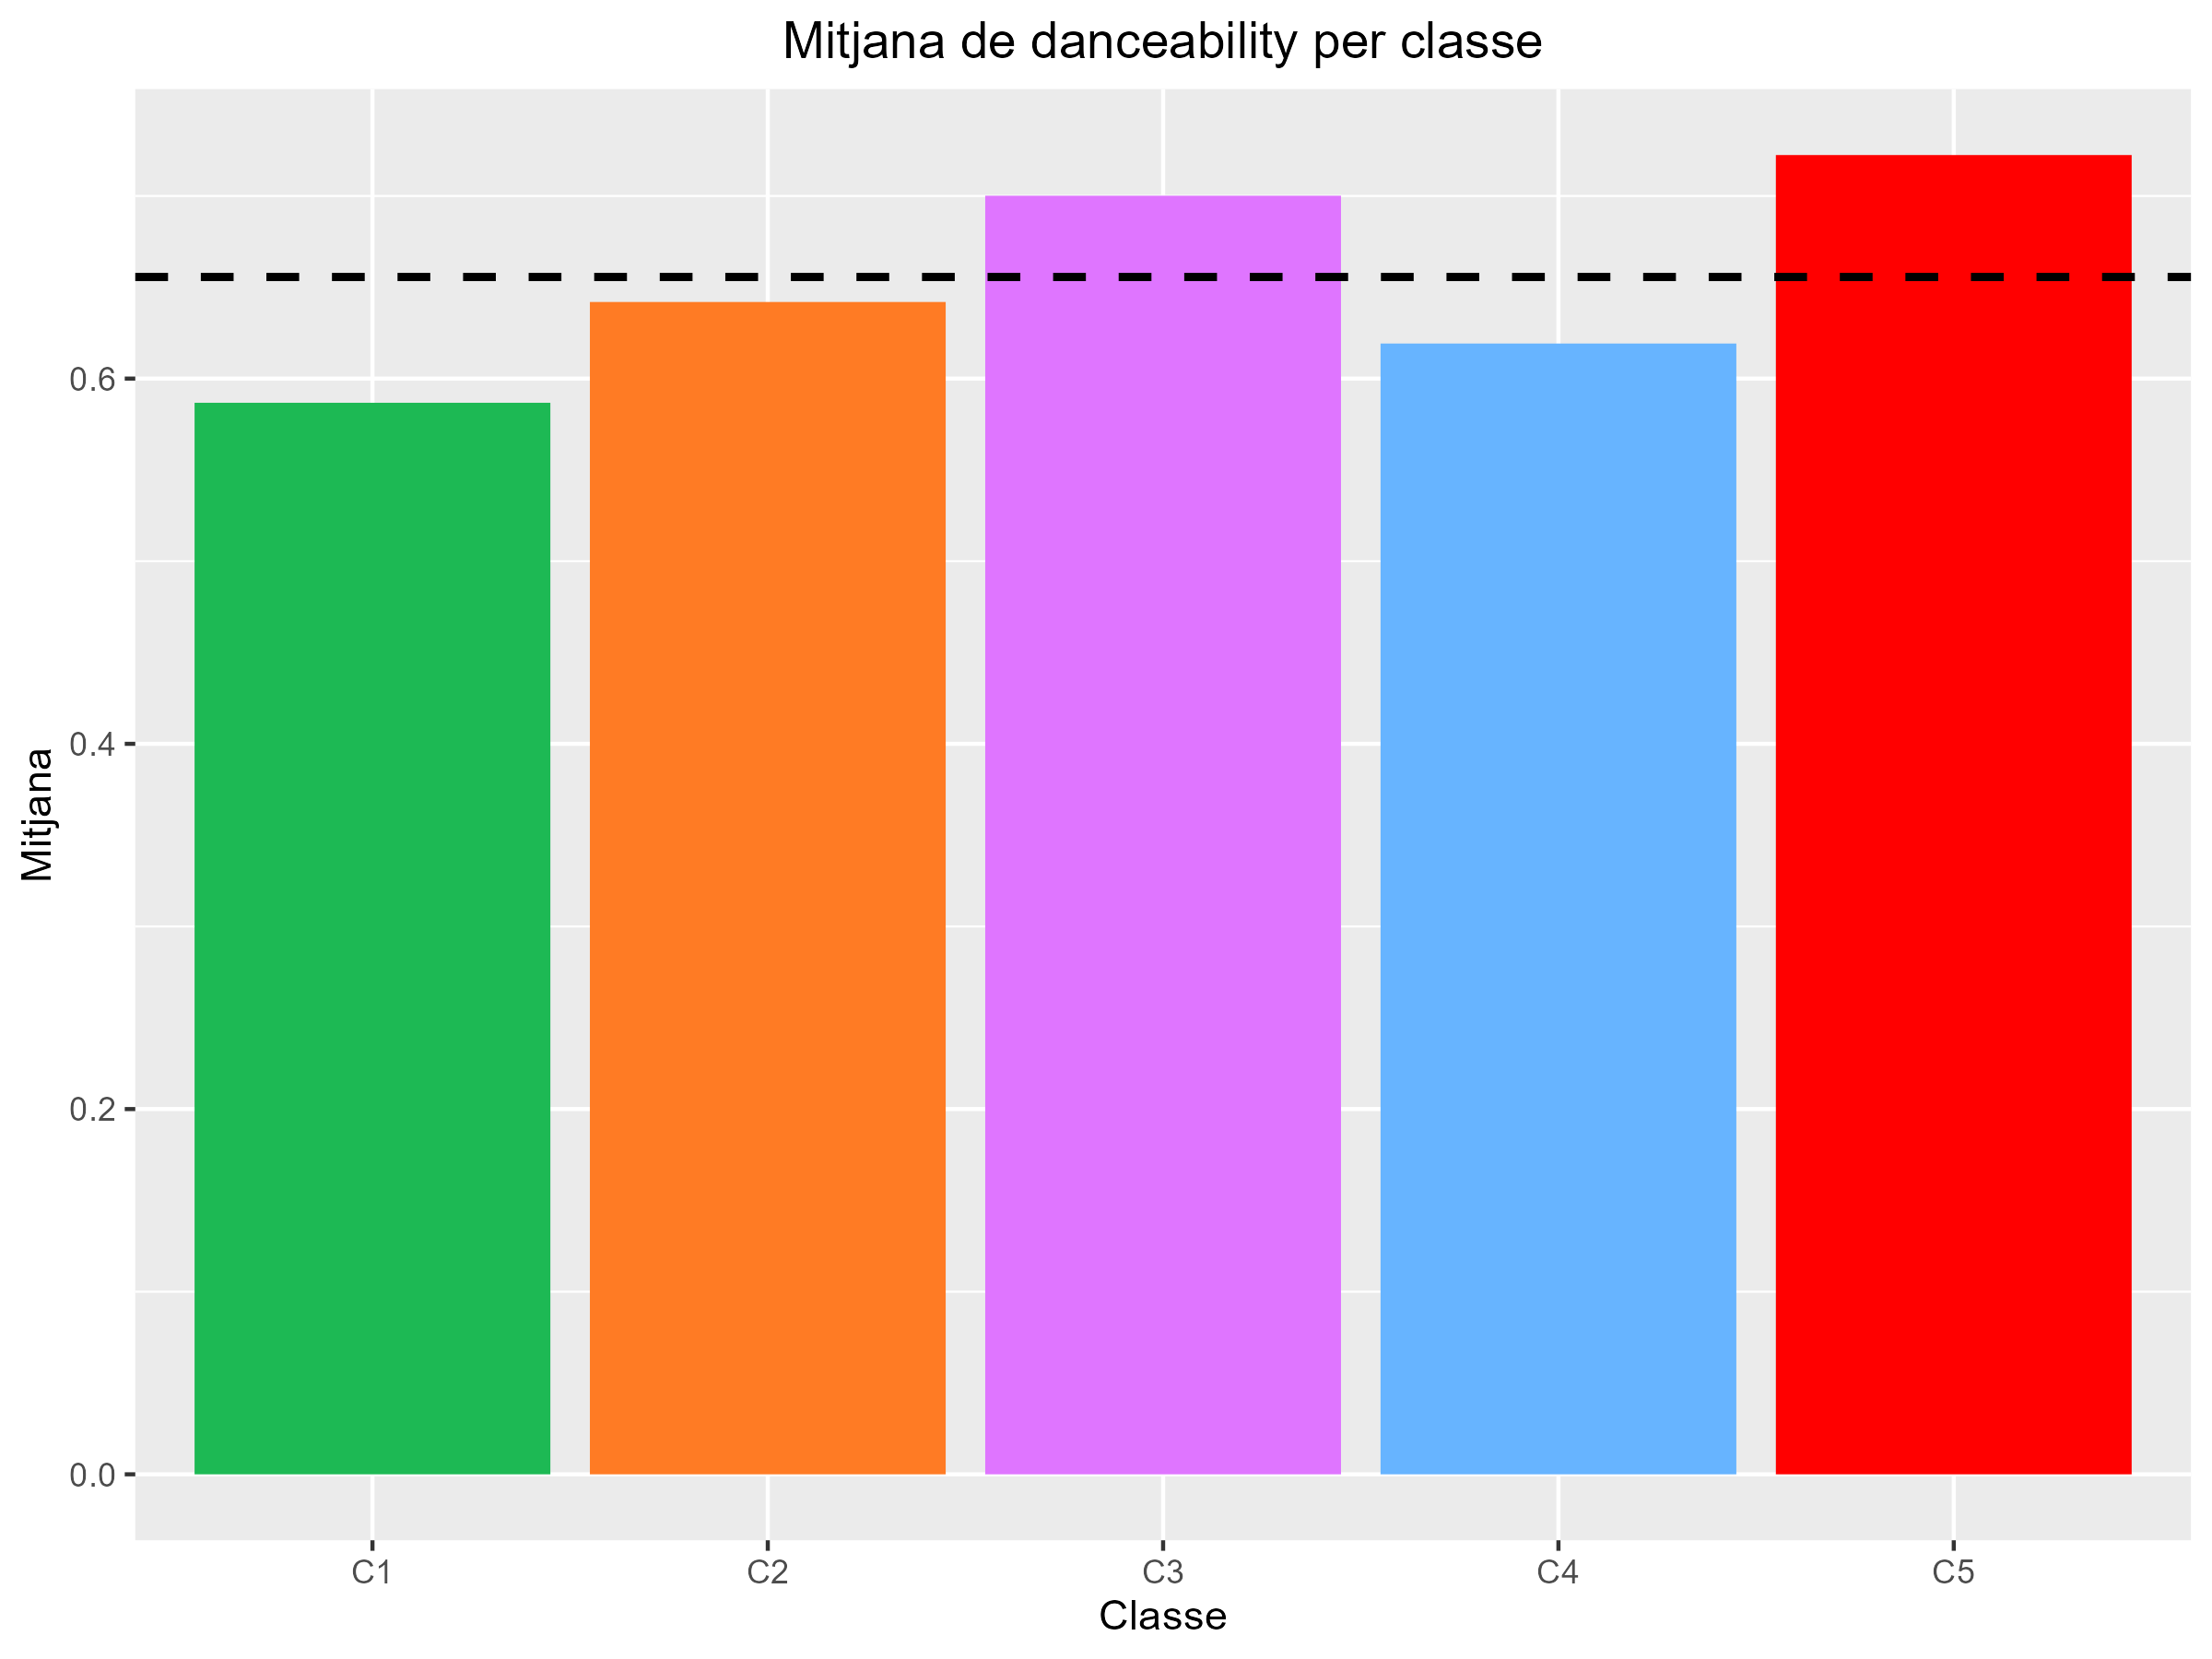
\includegraphics[width=0.95\linewidth]{Images/5_Profiling/numeriques/Num_BarPlot_danceability.png}
        \caption{Barplot amb les mitjanes \\ de danceability per clúster}
        \label{fig:Num_BarPlot_danceability}
    \end{minipage}%
    \begin{minipage}{.49\textwidth}
        \centering
        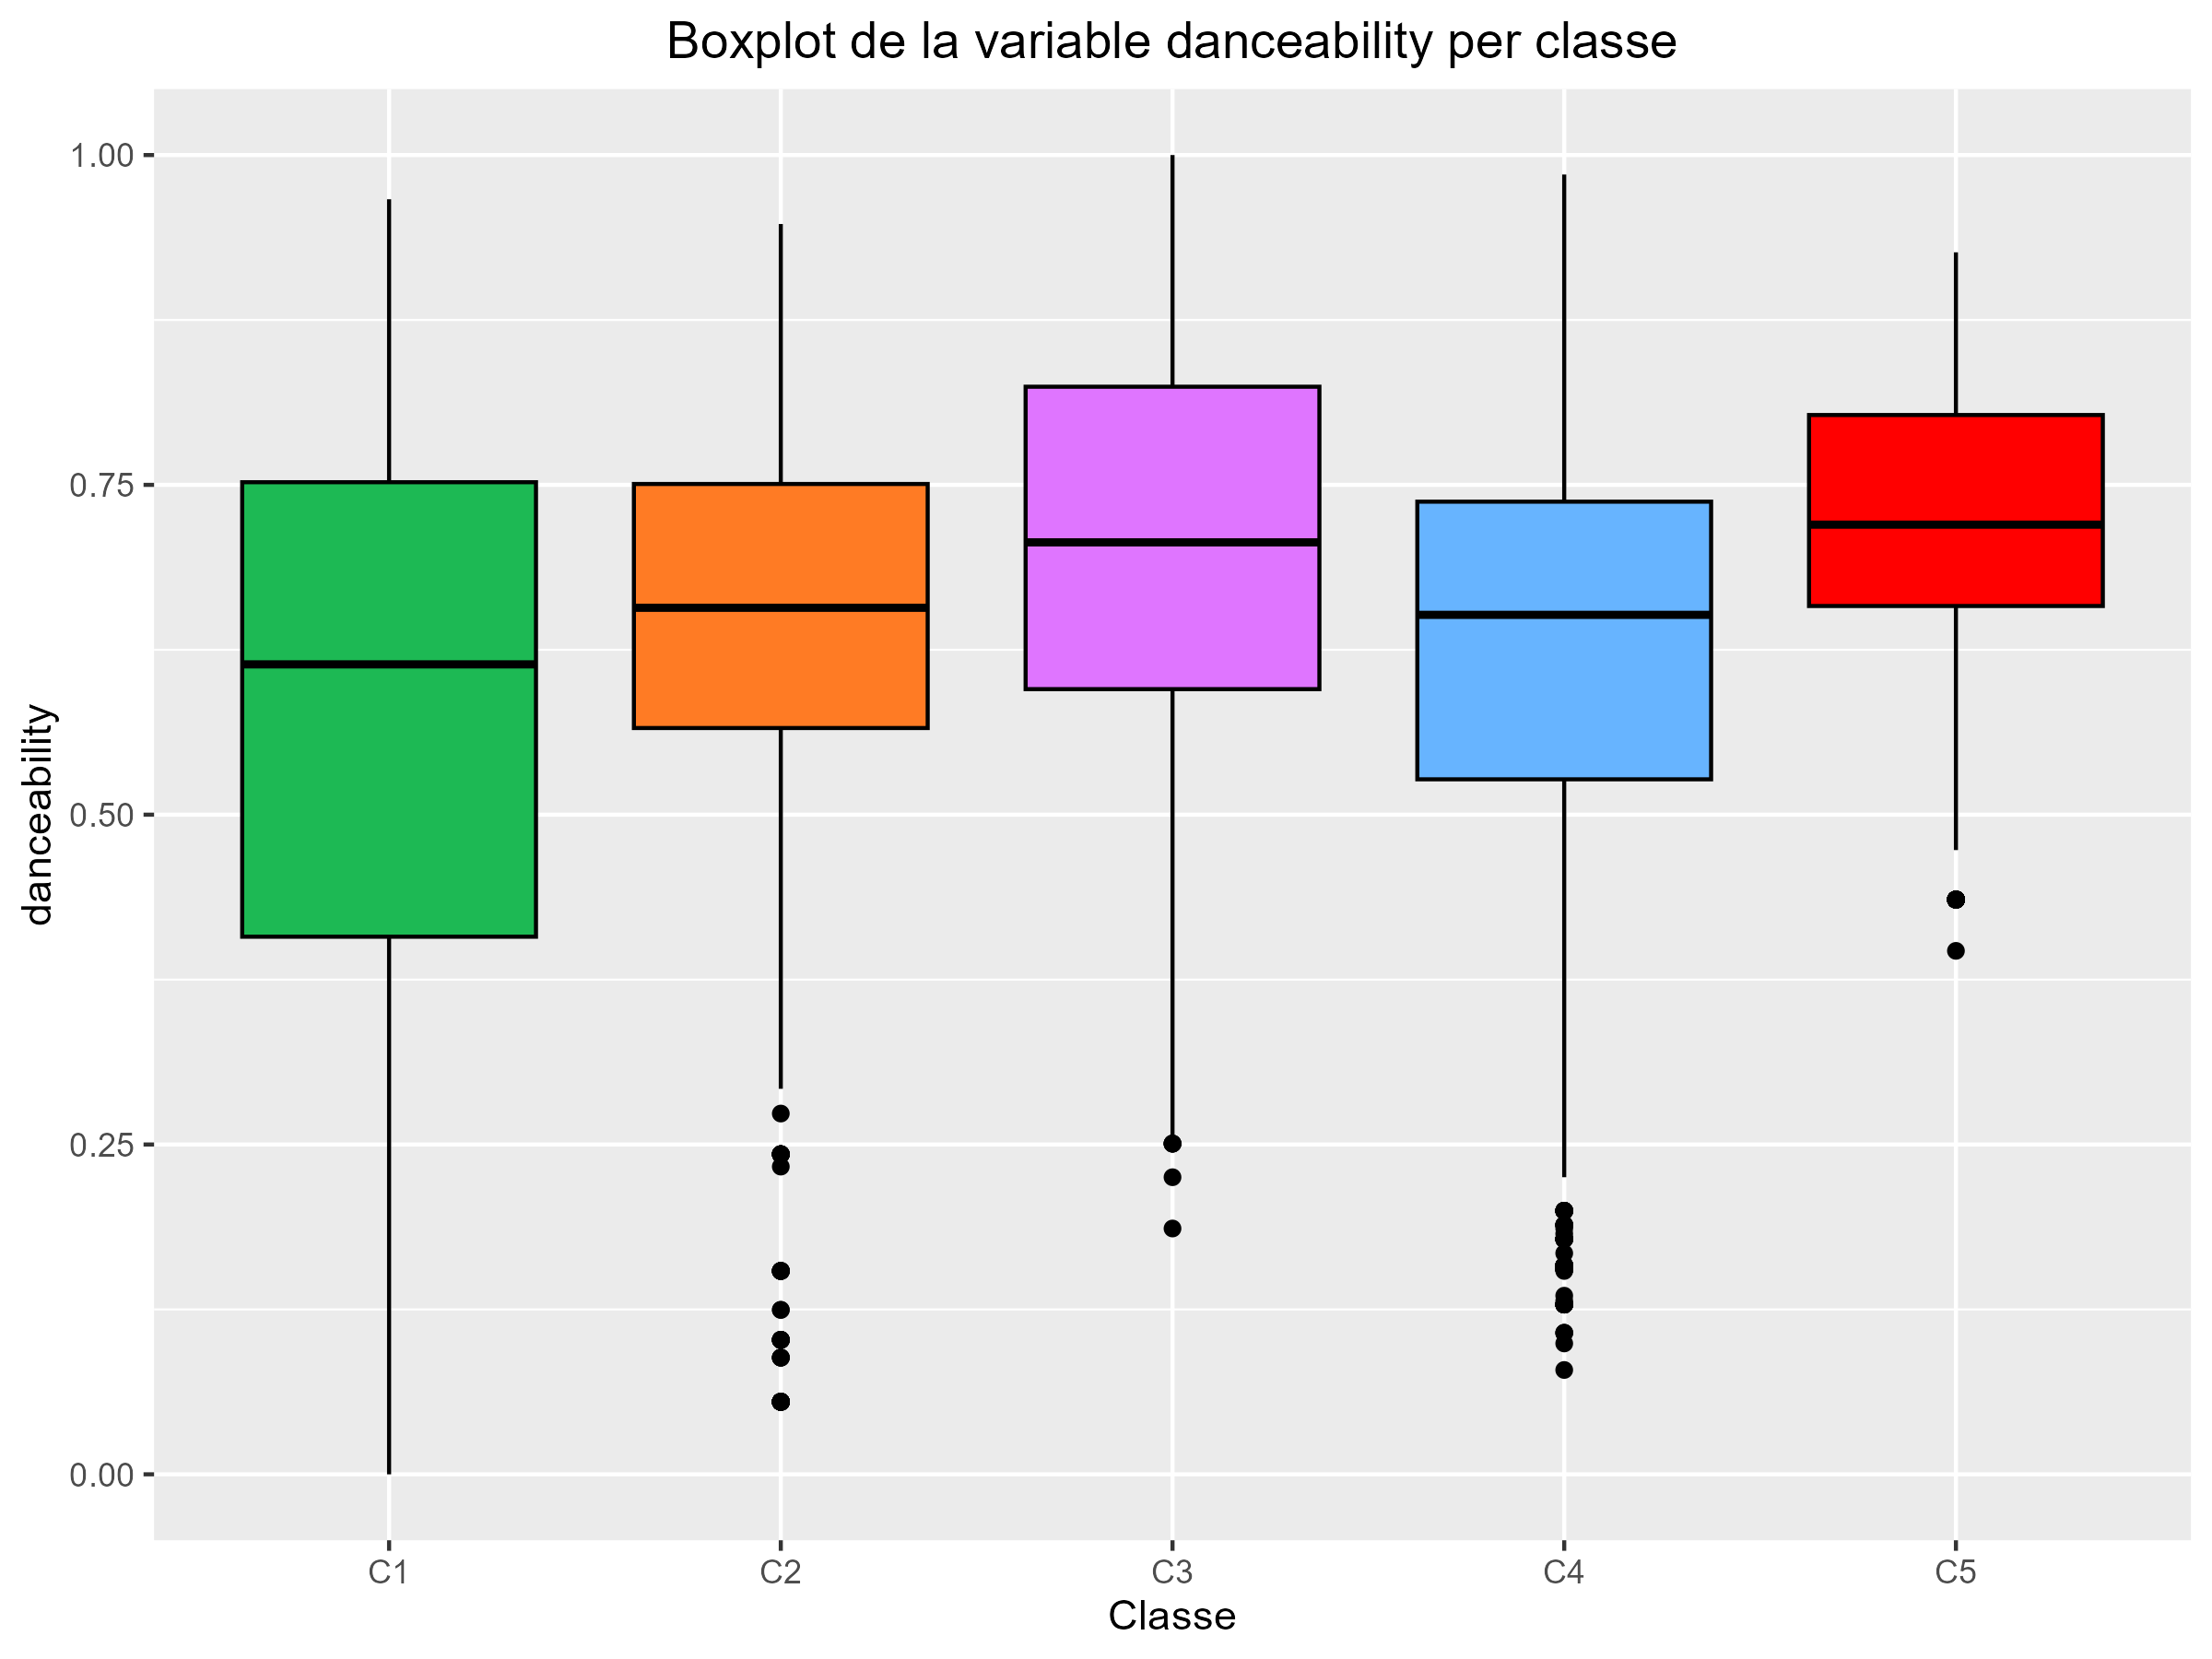
\includegraphics[width=0.95\linewidth]{Images/5_Profiling/numeriques/Num_BoxPlot_danceability.png}
        \caption{Boxplots de danceability per clúster}
        \label{fig:Num_BoxPlot_danceability}
    \end{minipage}%
\end{figure}
En el cas de danceability ens trobem que al primer clúster hi ha les cançons menys ballables en general. En canvi, en els clústers 3 i 5 hi ha cançons que són més ballables que la mitjana. 

\begin{figure}[H]
\centering
    \begin{minipage}{.49\textwidth}
        \centering
        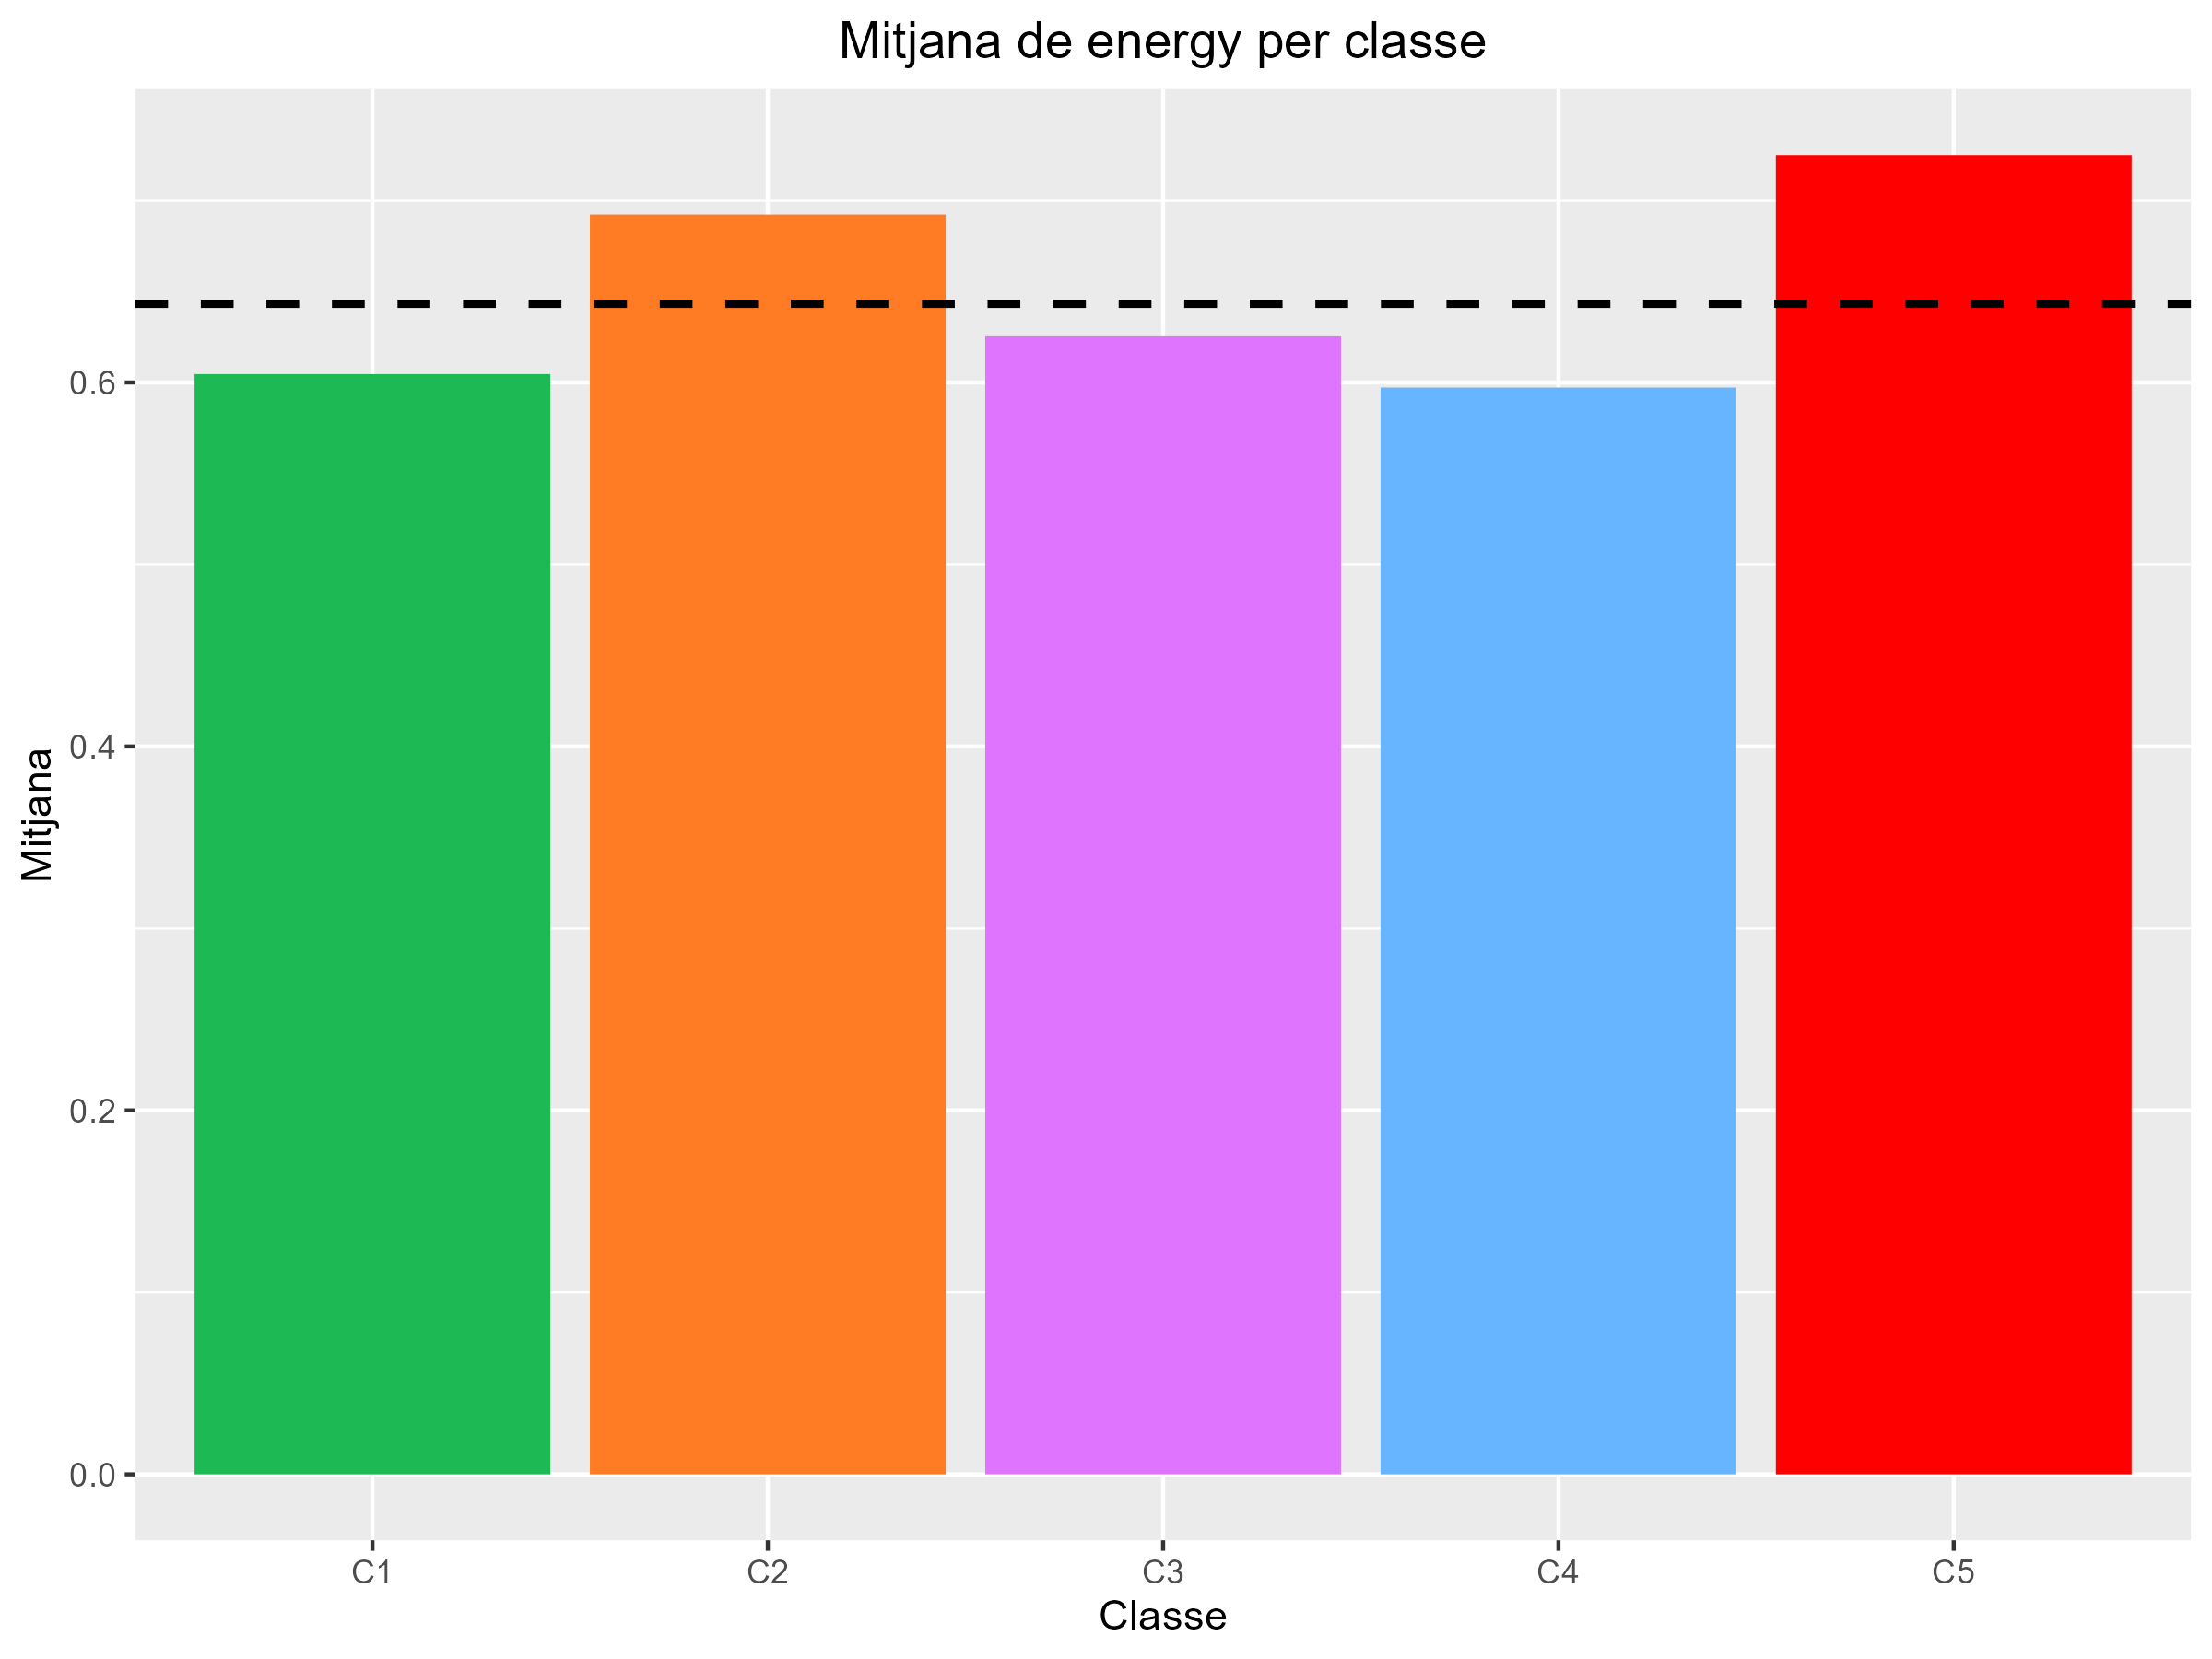
\includegraphics[width=0.95\linewidth]{Images/5_Profiling/numeriques/Num_BarPlot_energy.png}
        \caption{Barplot amb les mitjanes \\ de energy per clúster}
        \label{fig:Num_BarPlot_streams}
    \end{minipage}%
    \begin{minipage}{.49\textwidth}
        \centering
        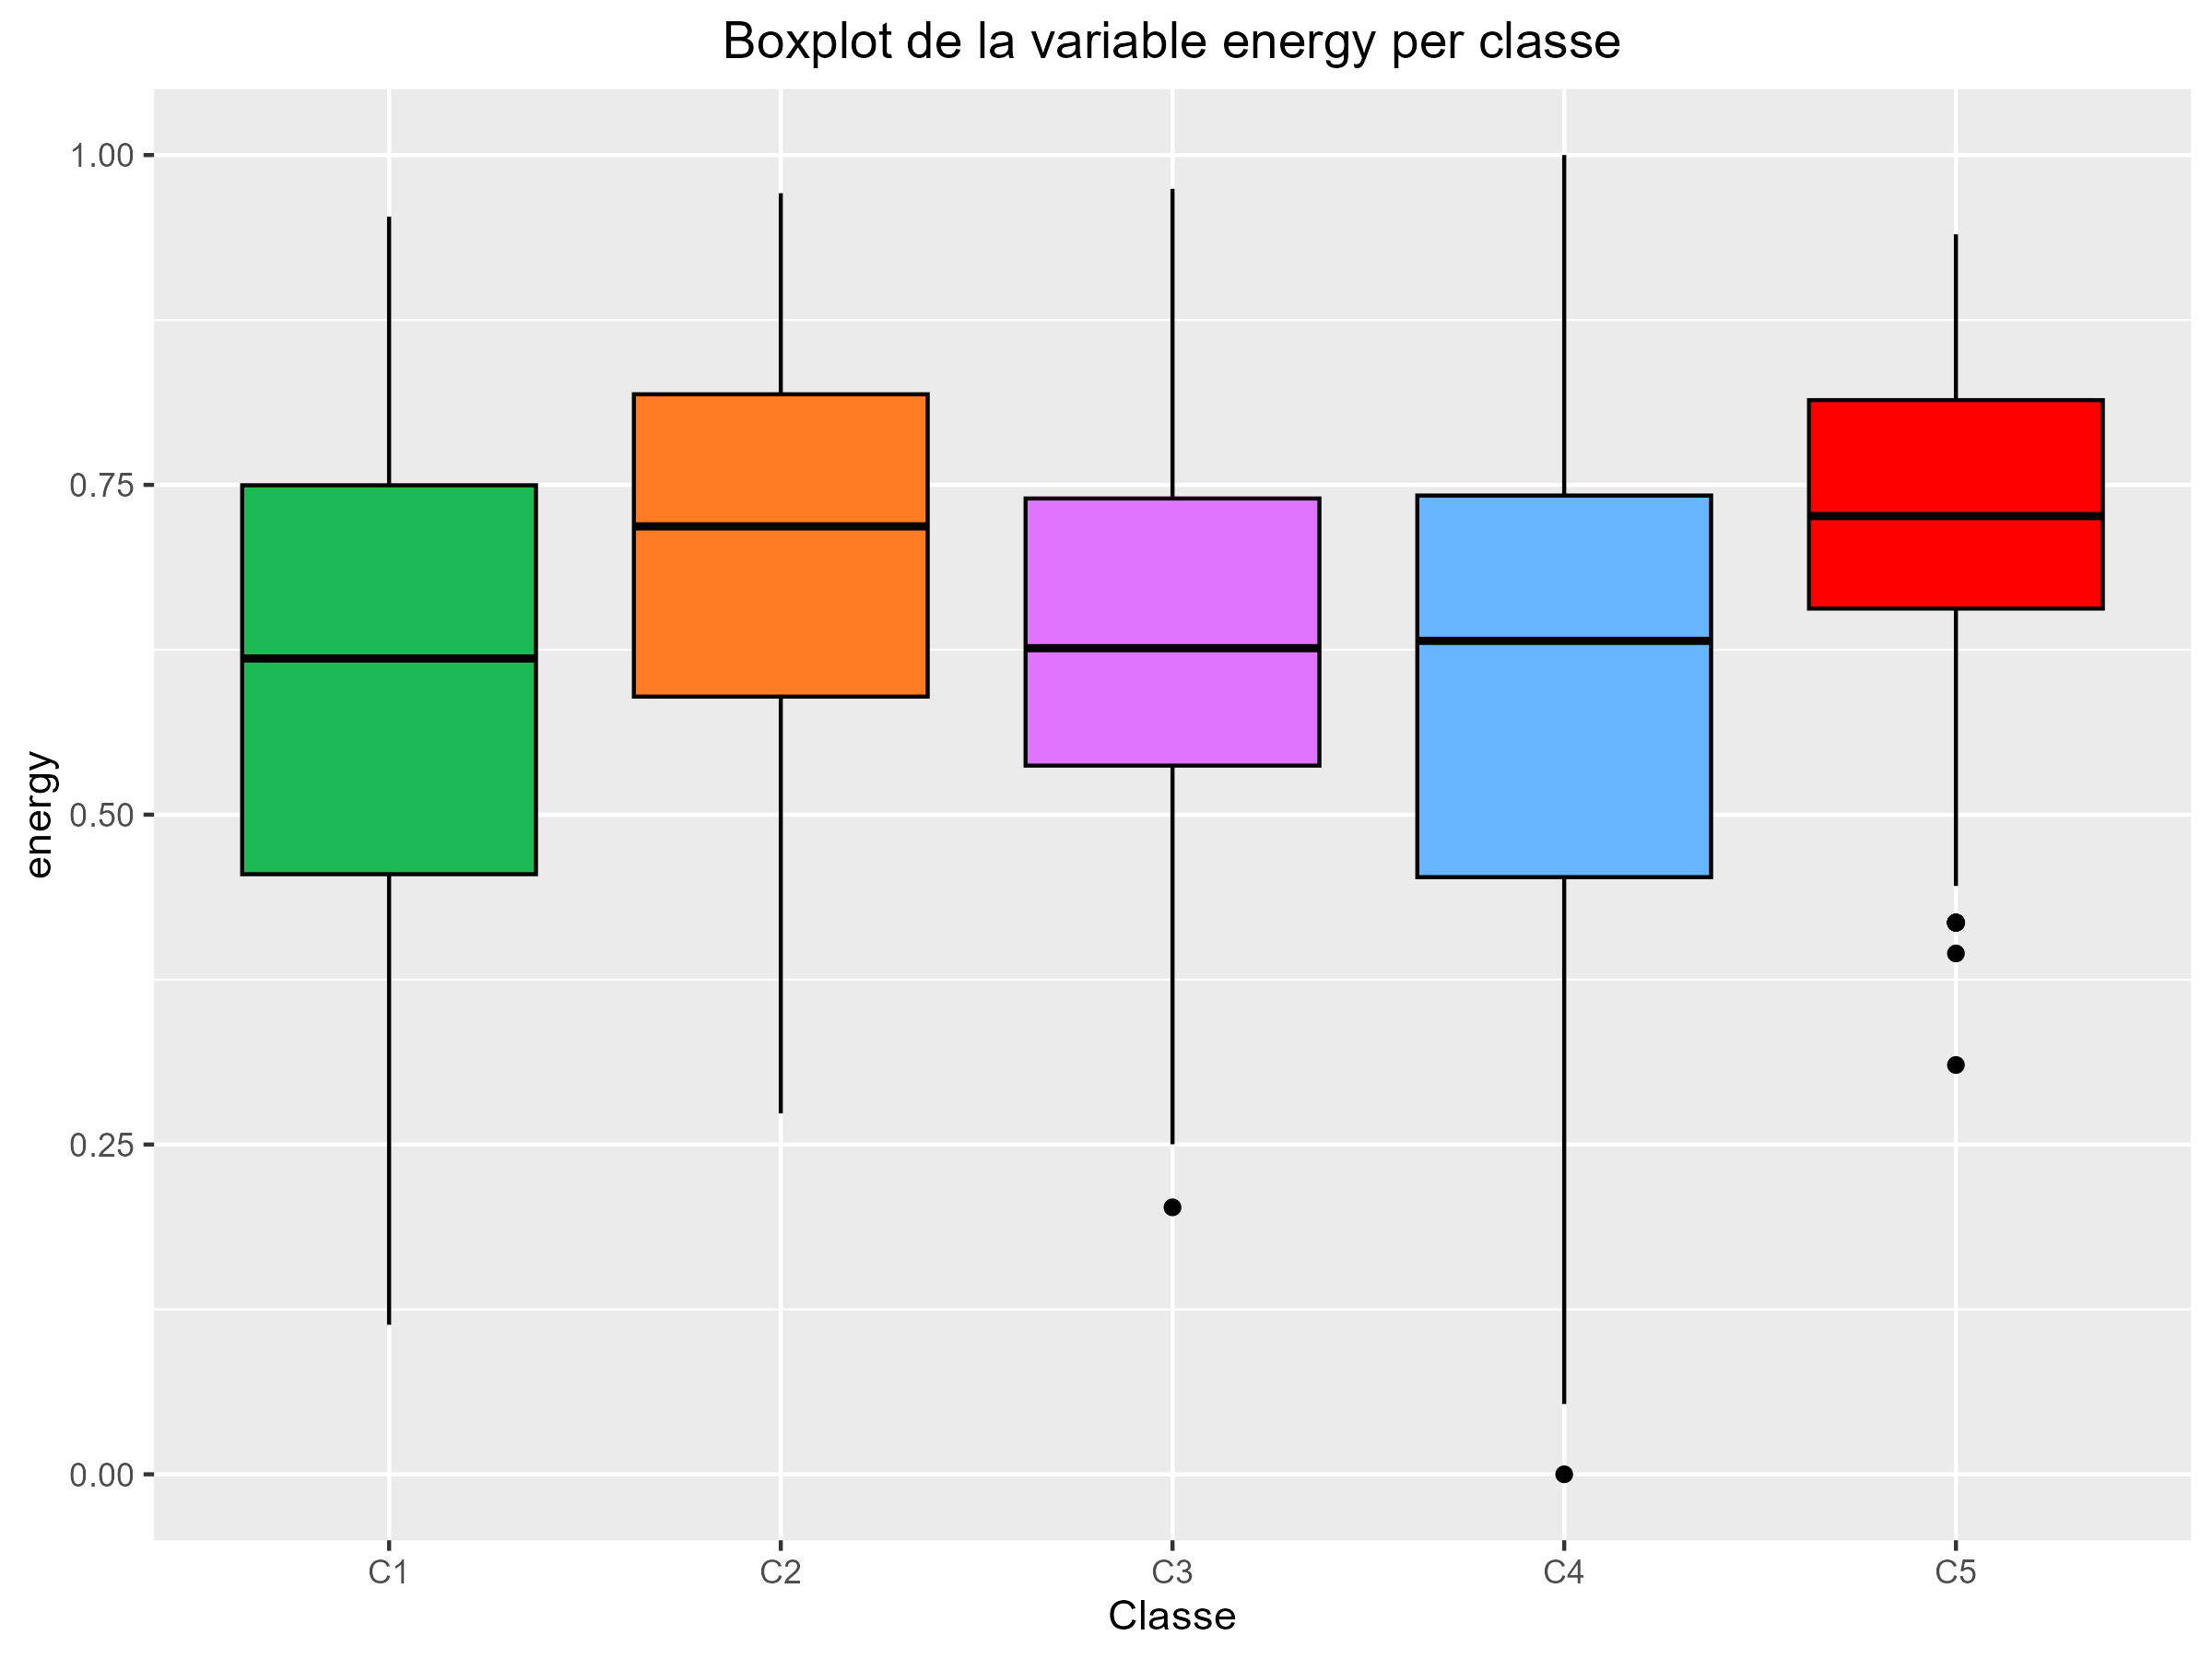
\includegraphics[width=0.95\linewidth]{Images/5_Profiling/numeriques/Num_BoxPlot_energy.png}
        \caption{Boxplots de energy per clúster}
        \label{fig:Num_BoxPlot_streams}
    \end{minipage}%
\end{figure}
En el cas de energy, el clúster 5 conté les cançons que són més energètiques, seguit del 2. Els altres tenen cançons menys energètiques però no molt menys que la mitjana. 
\begin{figure}[H]
\centering
    \begin{minipage}{.49\textwidth}
        \centering
        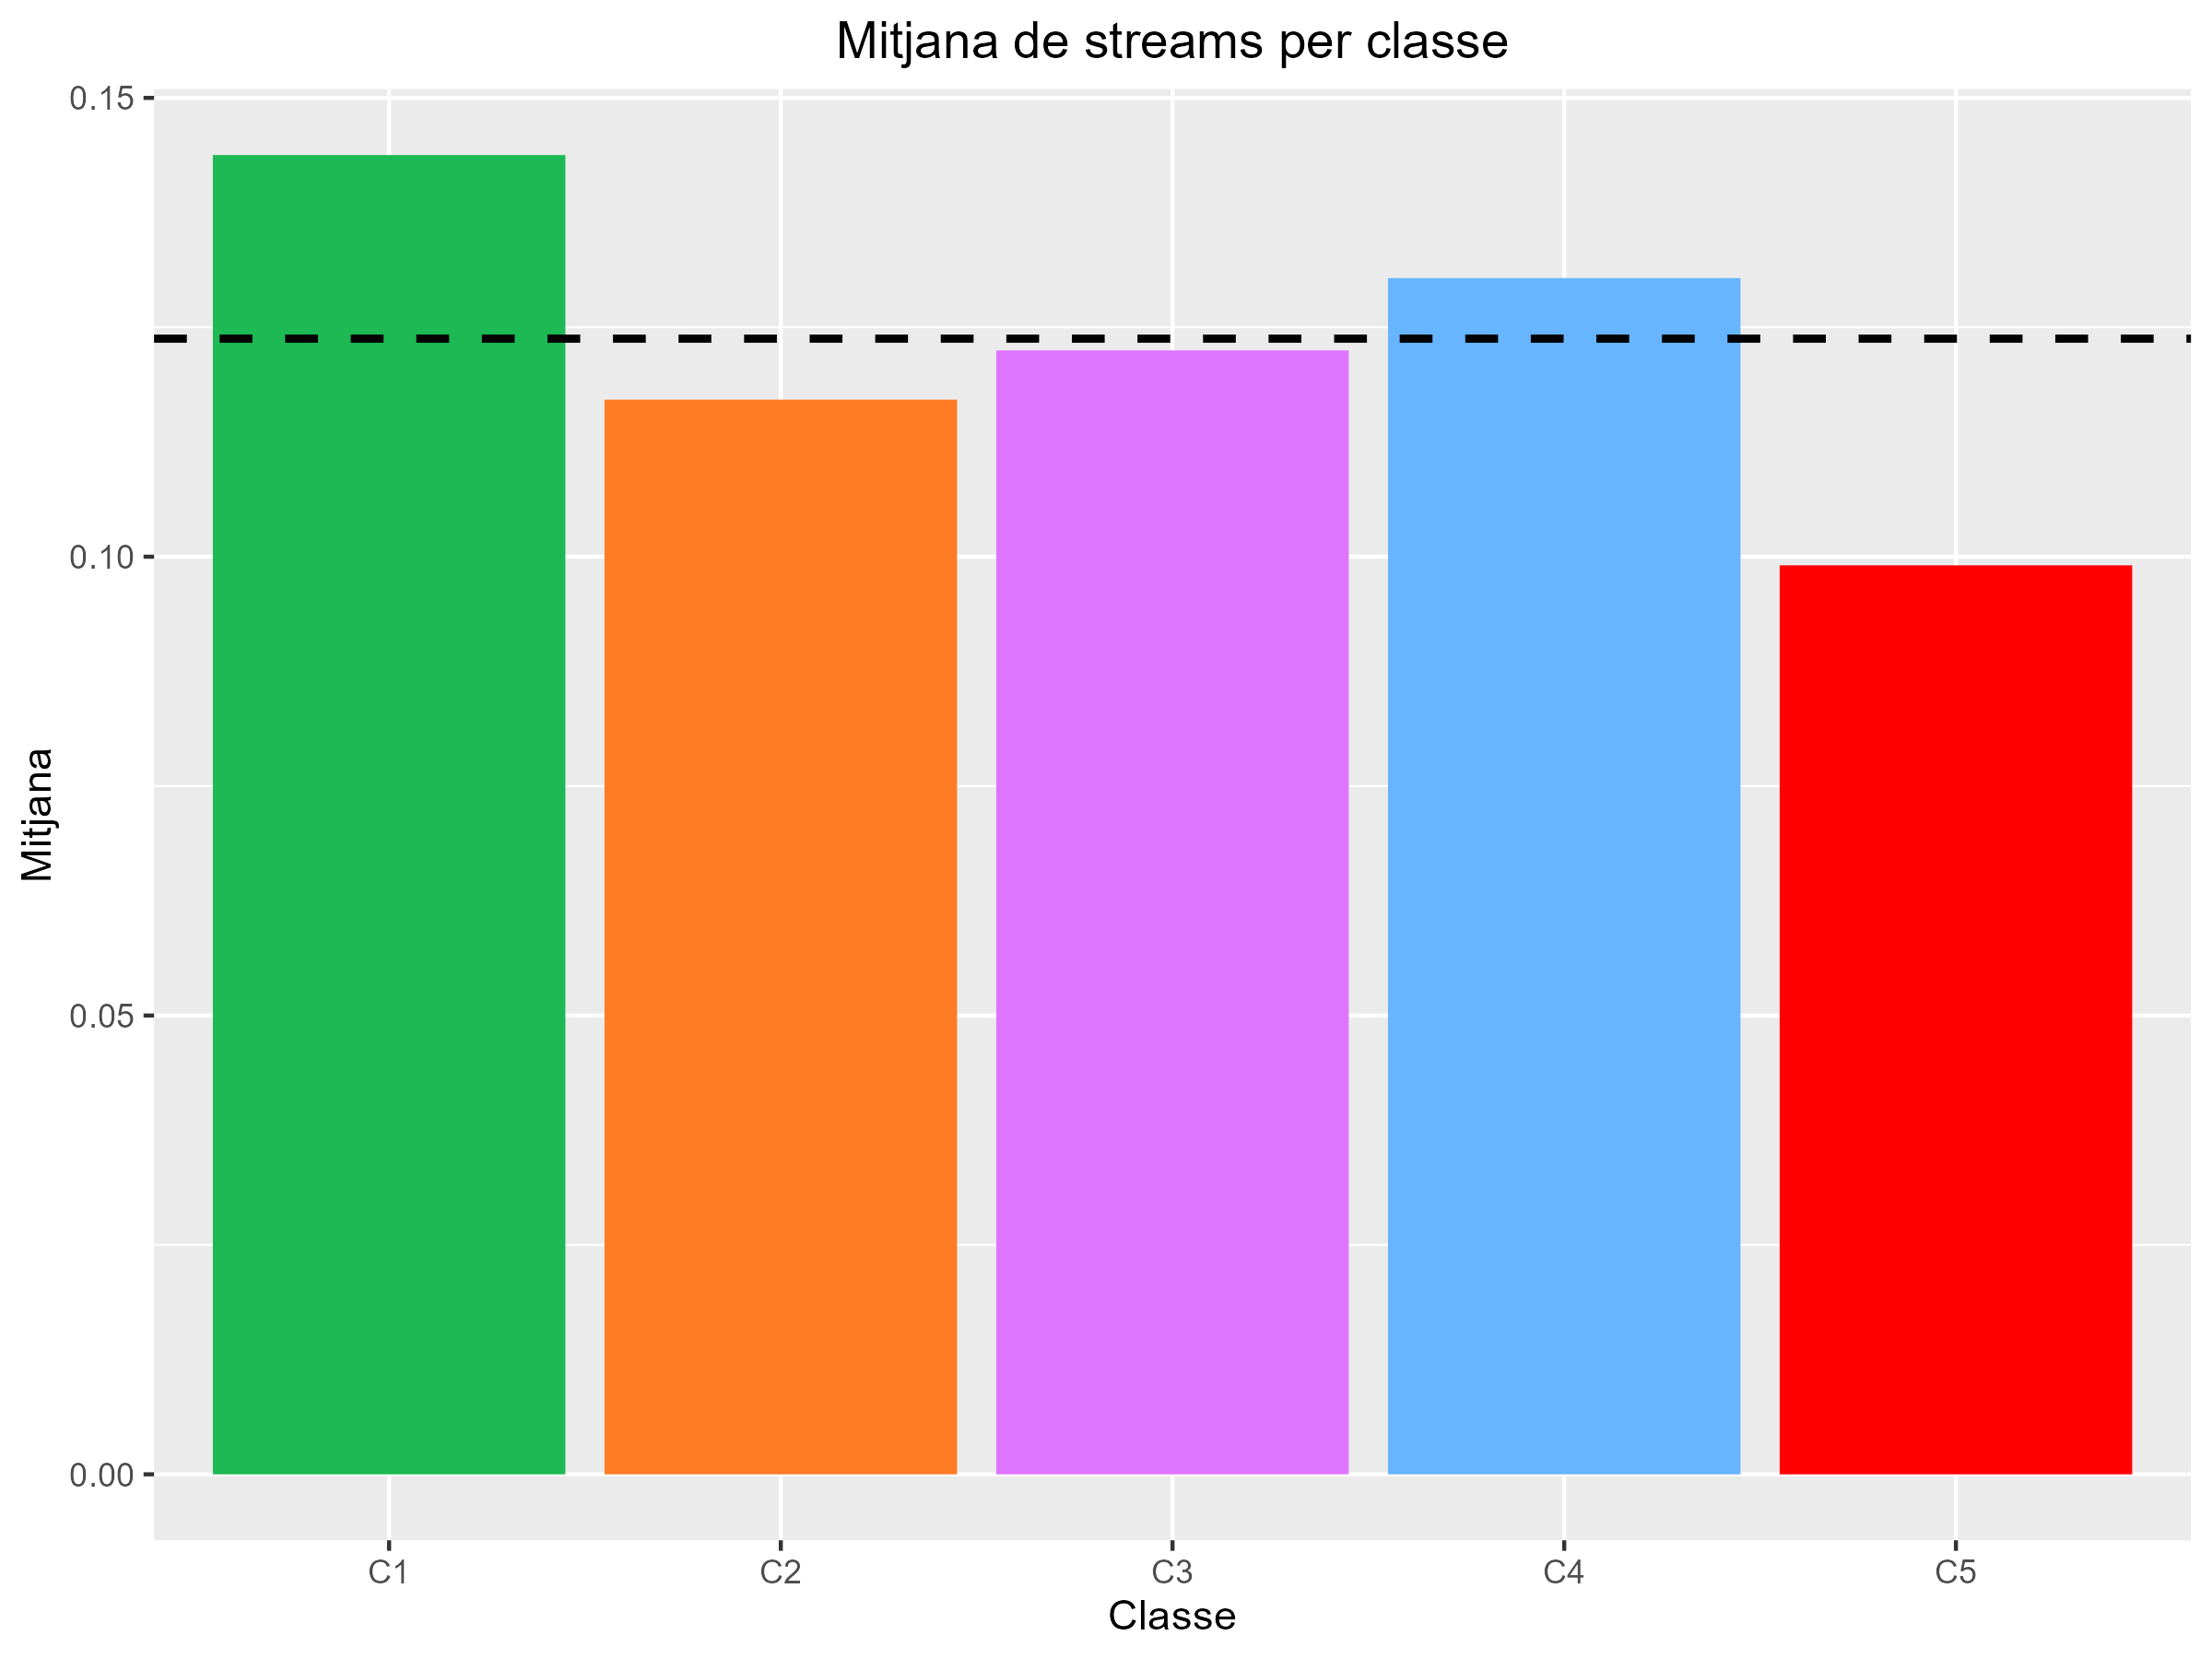
\includegraphics[width=0.95\linewidth]{Images/5_Profiling/numeriques/Num_BarPlot_streams.png}
        \caption{Barplot amb les mitjanes \\ de streams per clúster}
        \label{fig:Num_BarPlot_streams}
    \end{minipage}%
    \begin{minipage}{.49\textwidth}
        \centering
        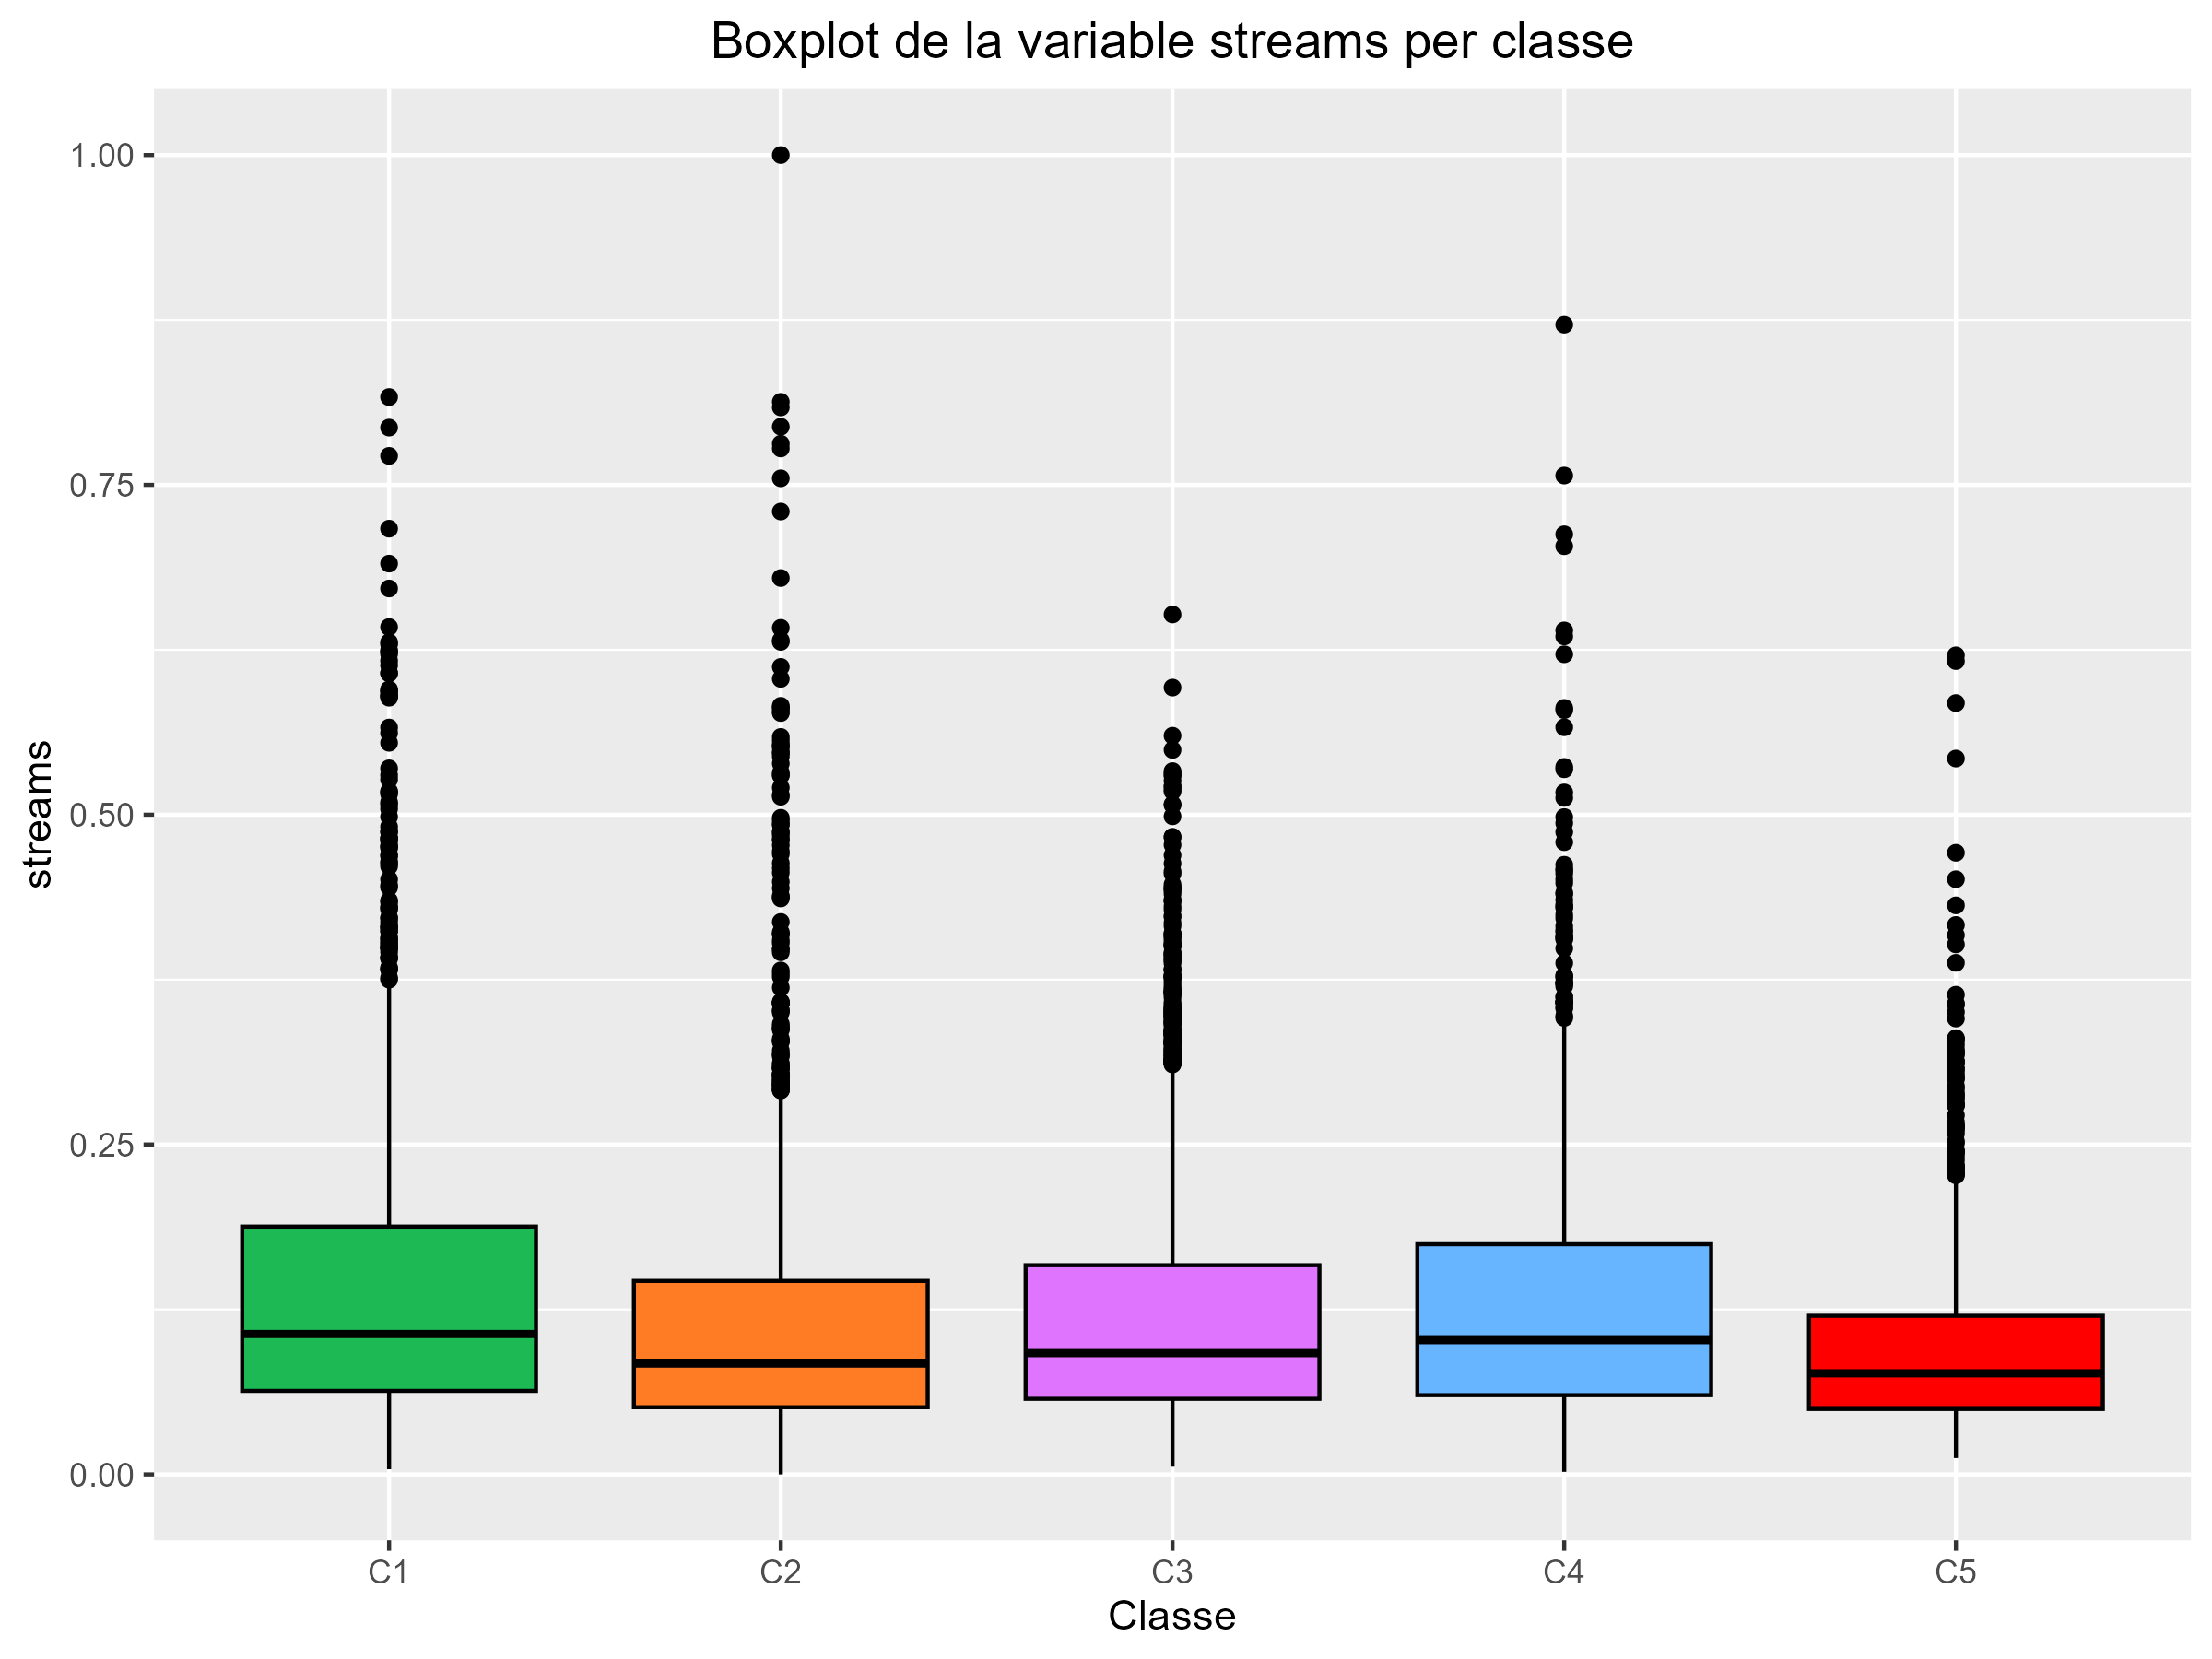
\includegraphics[width=0.95\linewidth]{Images/5_Profiling/numeriques/Num_BoxPlot_streams.png}
        \caption{Boxplots de streams per clúster}
        \label{fig:Num_BoxPlot_streams}
    \end{minipage}%
\end{figure}

A la variable streams ens trobem que la classe 1 té una mitjana relativament alta de streams. També veiem que el cinquè clúster és on hi ha les cançons amb una mitjana més baixa de reproduccions. Tot i això, ja veiem als boxplots que aquestes diferència no són extremadament significatives. 

\begin{figure}[H]
\centering
    \begin{minipage}{.49\textwidth}
        \centering
        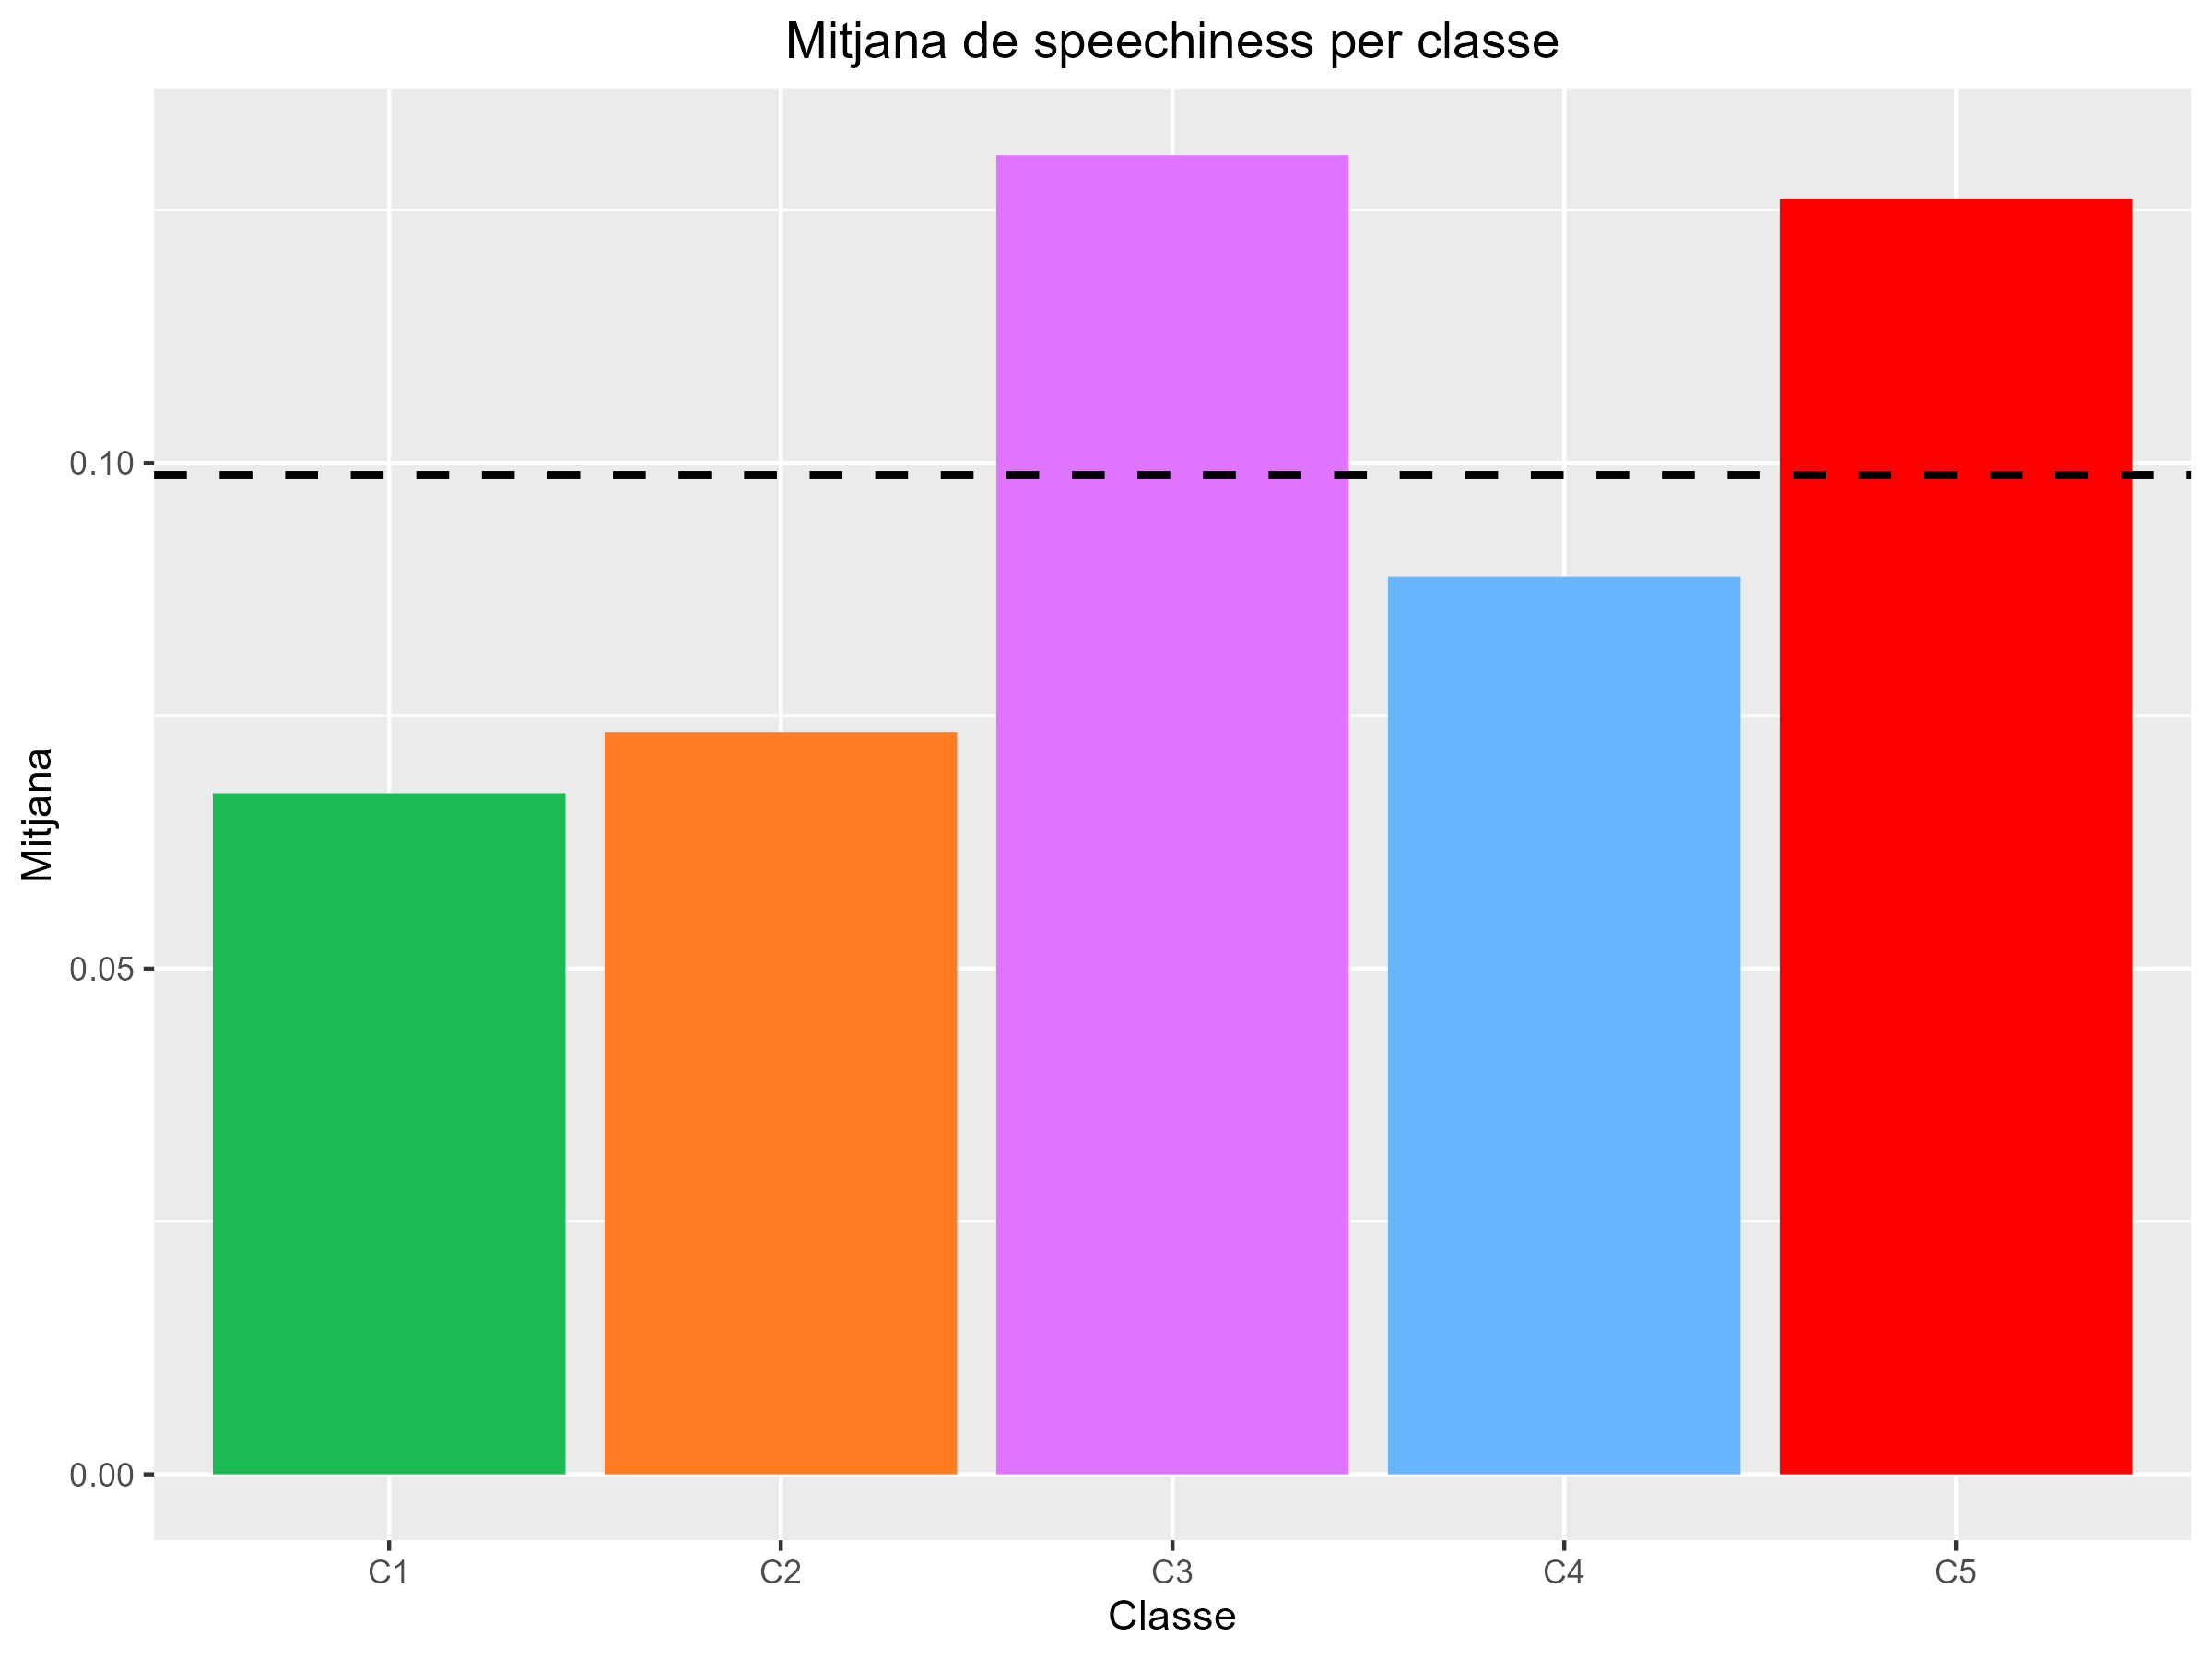
\includegraphics[width=0.95\linewidth]{Images/5_Profiling/numeriques/Num_BarPlot_speechiness.png}
        \caption{Barplot amb les mitjanes \\ de speechiness per clúster}
        \label{fig:Num_BarPlot_speechiness}
    \end{minipage}%
    \begin{minipage}{.49\textwidth}
        \centering
        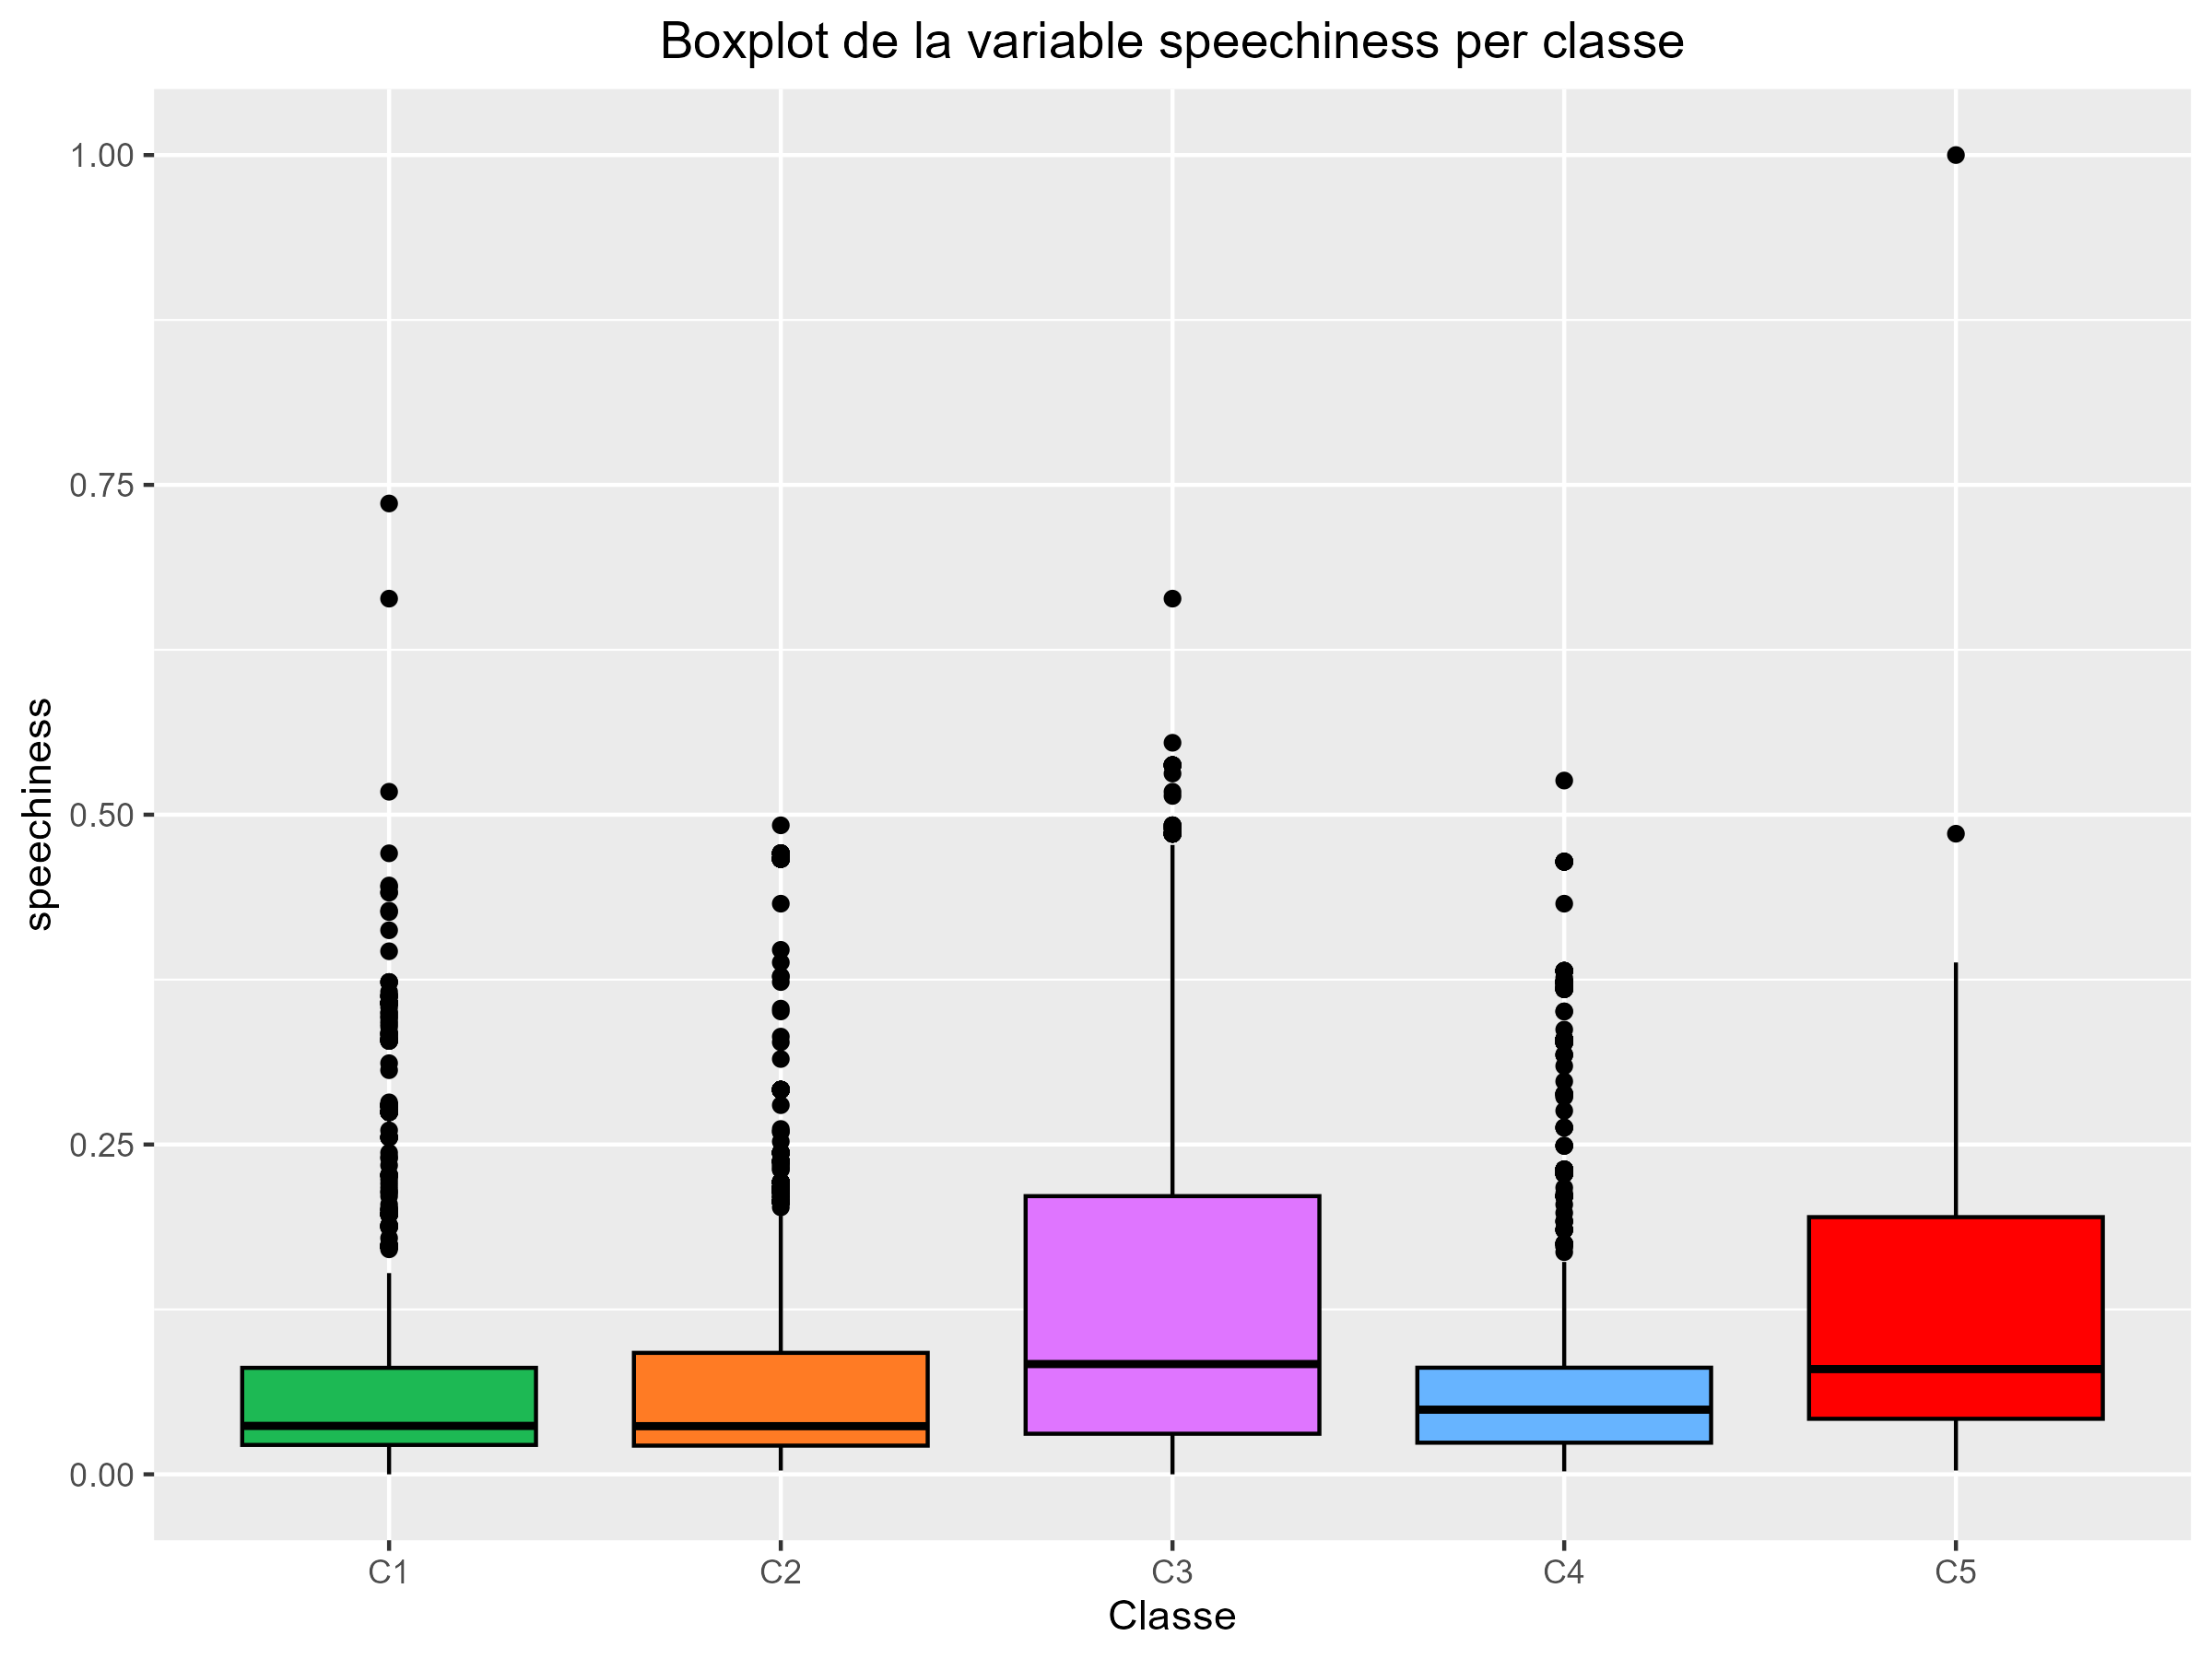
\includegraphics[width=0.95\linewidth]{Images/5_Profiling/numeriques/Num_BoxPlot_speechiness.png}
        \caption{Boxplots de speechiness per clúster}
        \label{fig:Num_BoxPlot_speechiness}
    \end{minipage}%
\end{figure}

Finalment, trobem que la variable speechiness ha influenciat de manera significativa als clústers formats. Amb molta diferència, les mitjanes de les classes 3 i 5 són molt més altes que la mitjana total, i això vol dir que allà es troben les cançons en les que predomina molt més la veu dels artistes. En canvi en els altres clústers, sobretot al primer i al segon, la mitjana és molt més baixa, indicant que allà estan les cançons en les que no hi ha tanta veu. 



\subsection{Variables categòriques}

En quant a les variables categòriques, farem per cada variable el test de chi-quadrat, que compara les distribucions de la variable categòrica amb la columna contenint els valors dels clústers (cada fila de la nostra base de dades a quin clúster pertany). S'avalua si hi ha un associació significativa entre la variable categòrica i els grups dels clústers proporcionant un p-valor.

Comencem a veure les variables que s'han utilitzat pel clustering.

\begin{figure}[H]
\centering
    \begin{minipage}{.49\textwidth}
        \centering
        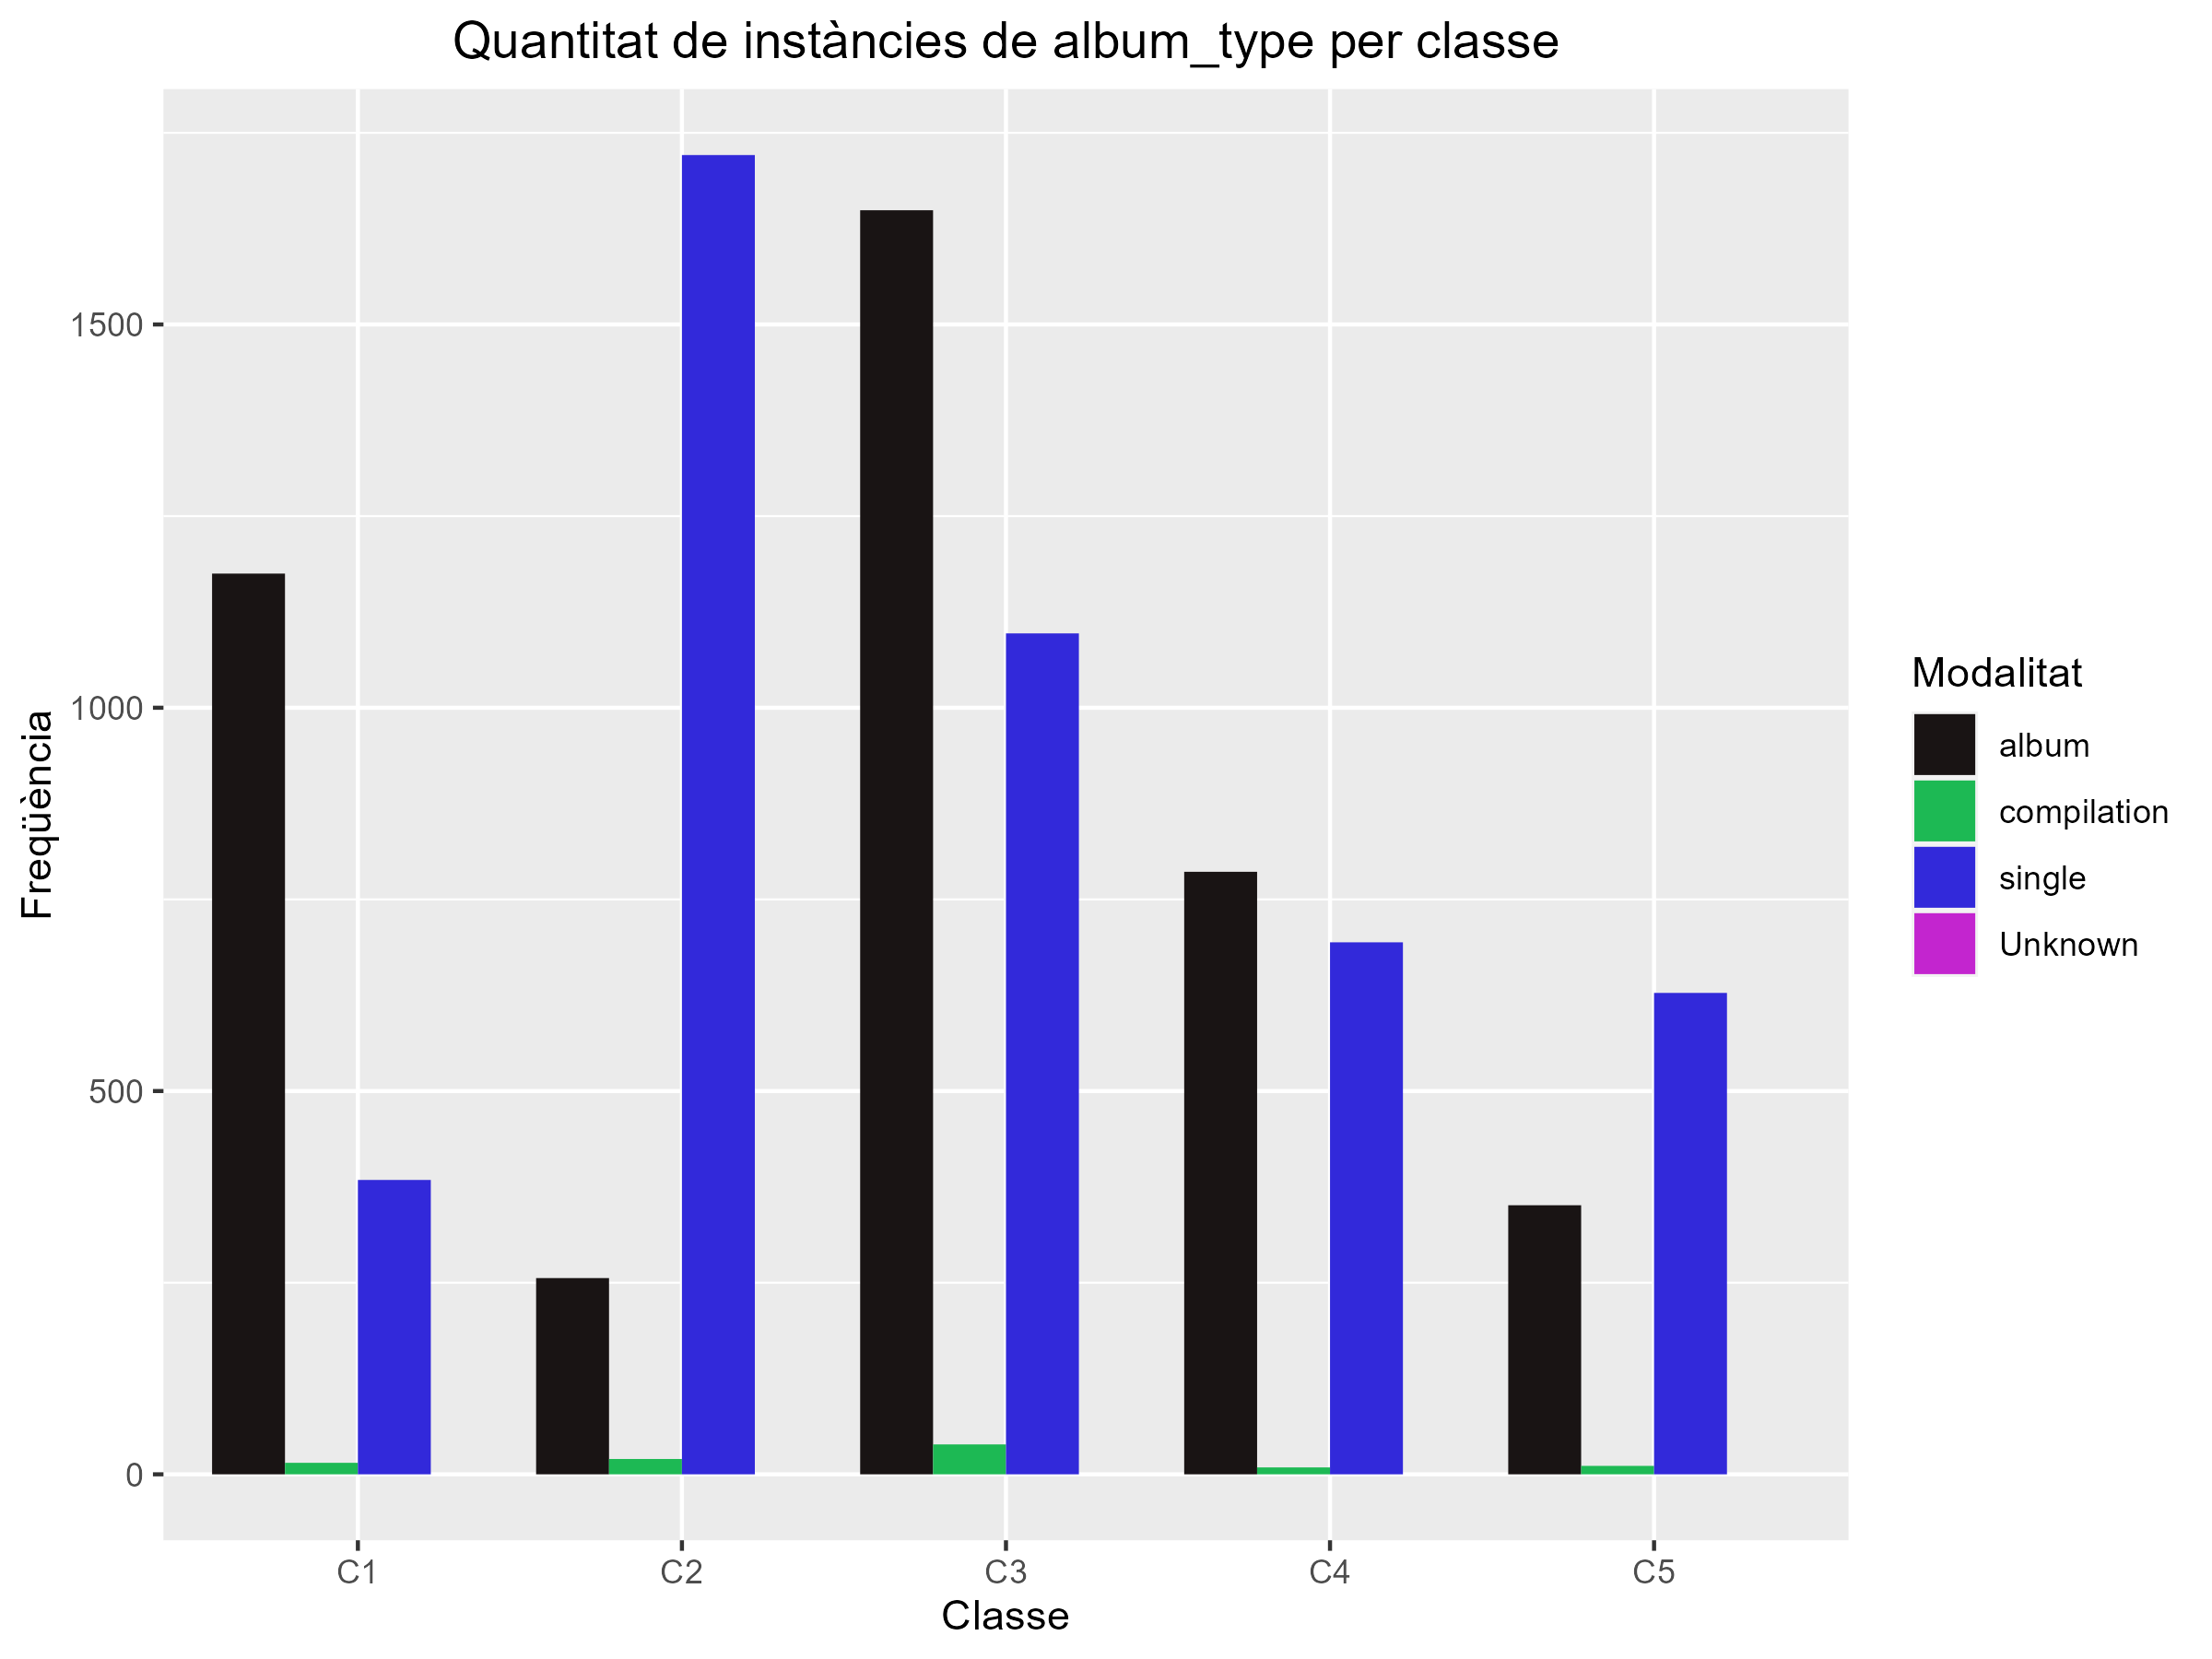
\includegraphics[width=0.95\linewidth]{Images/5_Profiling/categoriques/cat/Cat_BarPlot_album_type.png}
        \caption{Barplot amb els recomptes \\ d'album\_type per clúster}
        \label{fig:Cat_BarPlot_album_type}
    \end{minipage}%
    \begin{minipage}{.49\textwidth}
        \centering
        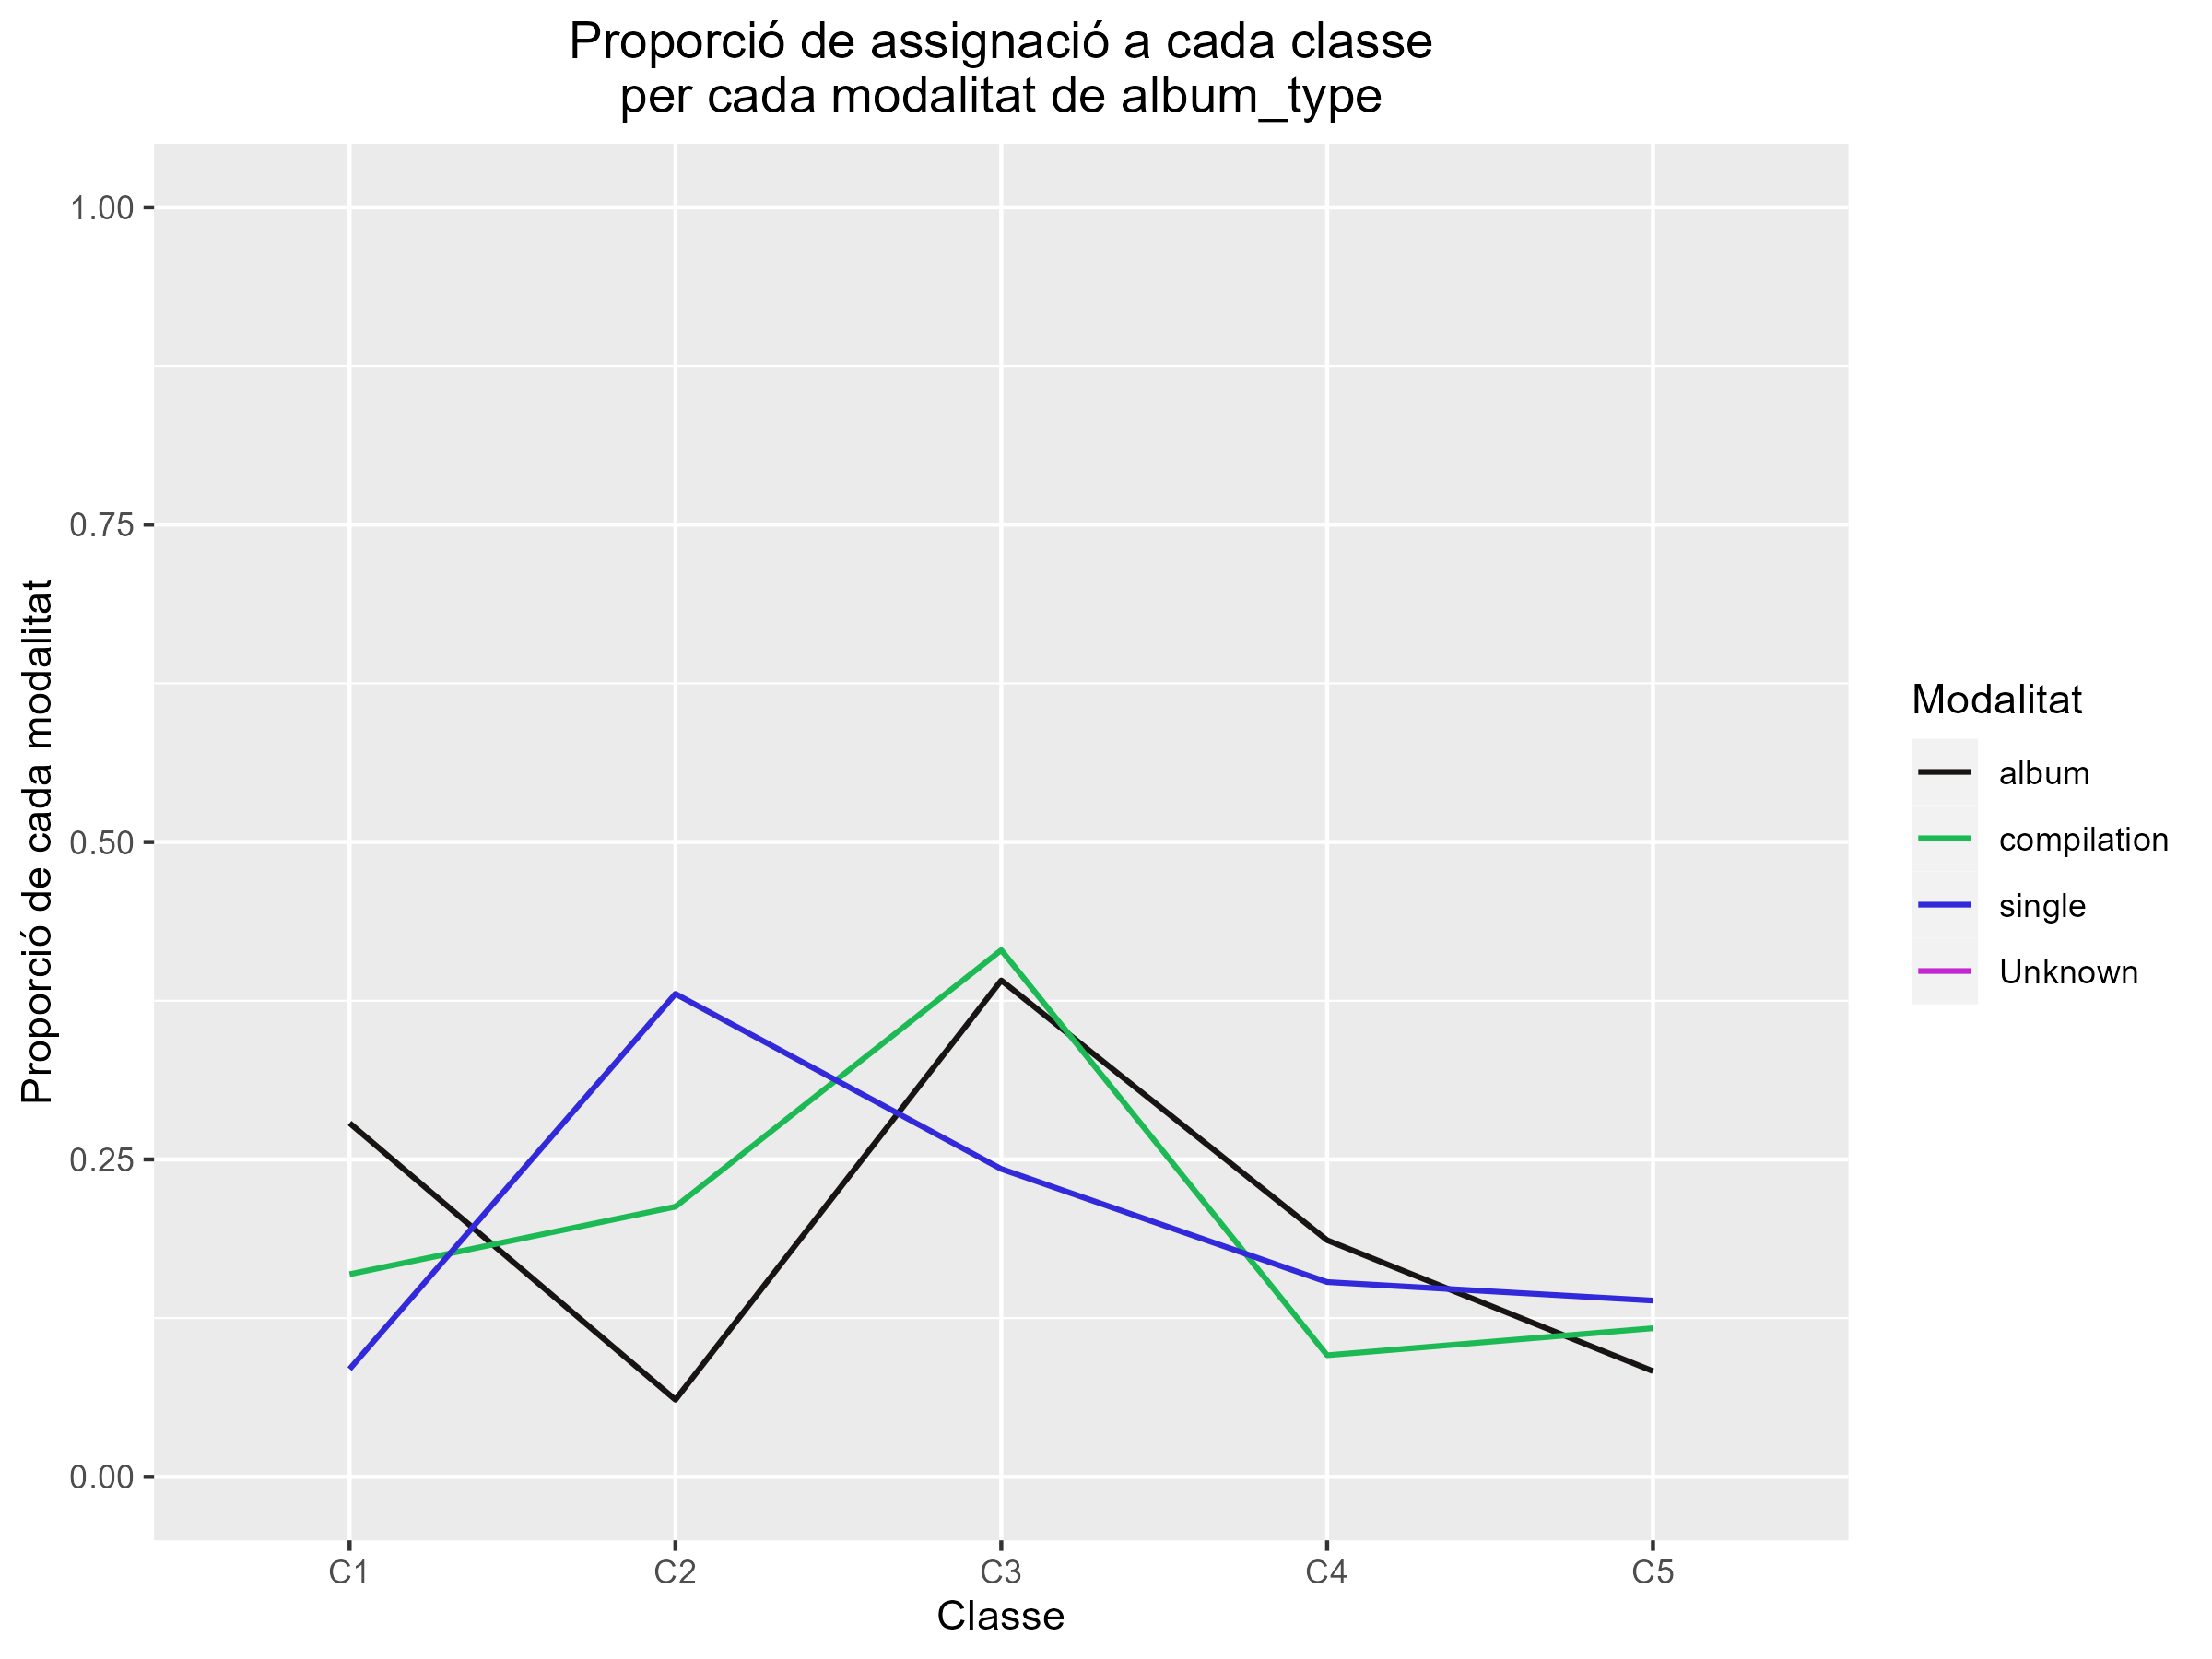
\includegraphics[width=0.95\linewidth]{Images/5_Profiling/categoriques/cat/Cat_SnakePlot_album_type.png}
        \caption{SnakePlot d'album\_type per clúster}
        \label{fig:Cat_SnakePlot_album_type}
    \end{minipage}%
\end{figure}

Com es pot veure als barplots, s'han posat la gran majoria de compilacions i albums a la classe tres. En canvi, al clúster 2 predominen amb molta diferència als singles. A les classes 4 i 5 veiem una proporció semblant de les diferents categories de la variable album\_type. Al clúster 1 també trobem un alt nombre d'instàncies d'album comparades amb les instàncies de single i compilation. Podriem dir que el clúster 3 amb la majoria d'instàncies d'album, podria tenir els valors d'album\_popularity més grans, la qual cosa caldrà seguir comprovant amb més variables. 

\begin{figure}[H]
\centering
    \begin{minipage}{.49\textwidth}
        \centering
        \includegraphics[width=0.95\linewidth]{Images/5_Profiling/categoriques/cat/Cat_BarPlot_christmas.png}
        \caption{Barplot amb els recomptes \\ de christmas per clúster}
        \label{fig:Cat_BarPlot_christmas}
    \end{minipage}%
    \begin{minipage}{.49\textwidth}
        \centering
        \includegraphics[width=0.95\linewidth]{Images/5_Profiling/categoriques/cat/Cat_SnakePlot_christmas.png}
        \caption{SnakePlot de christmas per clúster}
        \label{fig:Cat_SnakePlot_christmas}
    \end{minipage}%
\end{figure}

A la variable christmas, es pot veure que la majoria de les cançons nadalenques es troben al primer clúster. Tot i així també s'observen algunes instàncies al segon clúster. Cal destacar que en el dataset hi ha molt poques instàncies de cançons del gènere christmas, però el fet de que la majoria es concentrin en el clúster 1 ens dona una bona informació sobre aquell clúster. 

%cinema no aporta info

\begin{figure}[H]
\centering
    \begin{minipage}{.49\textwidth}
        \centering
        \includegraphics[width=0.95\linewidth]{Images/5_Profiling/categoriques/cat/Cat_BarPlot_collab.png}
        \caption{Barplot amb els recomptes \\ de collab per clúster}
        \label{fig:Cat_BarPlot_collab}
    \end{minipage}%
    \begin{minipage}{.49\textwidth}
        \centering
        \includegraphics[width=0.95\linewidth]{Images/5_Profiling/categoriques/cat/Cat_SnakePlot_collab.png}
        \caption{SnakePlot de collab per clúster}
        \label{fig:Cat_SnakePlot_collab}
    \end{minipage}%
\end{figure}

A la variable collab, podem obervar que en tots els clústers trobem instàncies tant de cançons amb colaboració com sense. Es pot destacar que als clúster 2 i 5, la majoria d'instàncies són cançons amb colaboració, en canvi els clústers 1 i 4, la majoria de cançons no tenen colaboració. Tot i així, al clúster 3 trobem pràcticament el mateix nombre de cançons amb colaboració i sense.

\begin{figure}[H]
\centering
    \begin{minipage}{.49\textwidth}
        \centering
        \includegraphics[width=0.95\linewidth]{Images/5_Profiling/categoriques/cat/Cat_BarPlot_electro.png}
        \caption{Barplot amb els recomptes \\ de electro per clúster}
        \label{fig:Cat_BarPlot_electro}
    \end{minipage}%
    \begin{minipage}{.49\textwidth}
        \centering
        \includegraphics[width=0.95\linewidth]{Images/5_Profiling/categoriques/cat/Cat_SnakePlot_electro.png}
        \caption{SnakePlot de electro per clúster}
        \label{fig:Cat_SnakePlot_electro}
wa    \end{minipage}%
\end{figure}

A la variable electro, es pot observar que la majoria d'instàncies de les cançons del gènere electro es troben en els clústers 2 i 4. En canvi, els clústers 1 i 3 no contenen pràcticament instàncies d'aquest gènere, a més, el clúster 5 no conté cap instància del gènere electro.

\begin{figure}[H]
\centering
    \begin{minipage}{.49\textwidth}
        \centering
        \includegraphics[width=0.95\linewidth]{Images/5_Profiling/categoriques/cat/Cat_BarPlot_explicit.png}
        \caption{Barplot amb els recomptes \\ de explicit per clúster}
        \label{fig:Cat_BarPlot_explicit}
    \end{minipage}%
    \begin{minipage}{.49\textwidth}
        \centering
        \includegraphics[width=0.95\linewidth]{Images/5_Profiling/categoriques/cat/Cat_SnakePlot_explicit.png}
        \caption{SnakePlot de explicit per clúster}
        \label{fig:Cat_SnakePlot_explicit}
    \end{minipage}%
\end{figure}

A la variable explicit, trobem que la gran majoria de cançons explícites es troben al tercer clúster. Tot i així, els altres clústers també tenen instàncies de cançons explícites, encara que contenen moltes més instàncies de cançons no explícites que d'explícites.

\begin{figure}[H]
\centering
    \begin{minipage}{.49\textwidth}
        \centering
        \includegraphics[width=0.95\linewidth]{Images/5_Profiling/categoriques/cat/Cat_BarPlot_hip_hop.png}
        \caption{Barplot amb els recomptes \\ de hip-hop per clúster}
        \label{fig:Cat_BarPlot_hip_hop}
    \end{minipage}%
    \begin{minipage}{.49\textwidth}
        \centering
        \includegraphics[width=0.95\linewidth]{Images/5_Profiling/categoriques/cat/Cat_SnakePlot_hip_hop.png}
        \caption{SnakePlot de hip-hop per clúster}
        \label{fig:Cat_SnakePlot_hip_hop}
    \end{minipage}%
\end{figure}

A la variable hip\_hop trobem que la majoria d'instàncies es troben en el tercer clúster, tot i així, al cinquè clúster també trobem gran part d'aquestes. En canvi, als altres clústers pràcticament no trobem cap cançó del gènere hip hop.

\begin{figure}[H]
\centering
    \begin{minipage}{.49\textwidth}
        \centering
        \includegraphics[width=0.95\linewidth]{Images/5_Profiling/categoriques/cat/Cat_BarPlot_latino.png}
        \caption{Barplot amb els recomptes \\ de latino per clúster}
        \label{fig:Cat_BarPlot_latino}
    \end{minipage}%
    \begin{minipage}{.49\textwidth}
        \centering
        \includegraphics[width=0.95\linewidth]{Images/5_Profiling/categoriques/cat/Cat_SnakePlot_latino.png}
        \caption{SnakePlot de latino per clúster}
        \label{fig:Cat_SnakePlot_latino}
    \end{minipage}%
\end{figure}

A la variable latino, es pot observar que pràcticament el 90\% de les cançons de gènere latino es troben en el cinquè clúster. Mentre que a la resta de clústers no trobem pràcticament cançons d'aquest gènere.

\begin{figure}[H]
\centering
    \begin{minipage}{.49\textwidth}
        \centering
        \includegraphics[width=0.95\linewidth]{Images/5_Profiling/categoriques/cat/Cat_BarPlot_rock.png}
        \caption{Barplot amb els recomptes \\ de rock per clúster}
        \label{fig:Cat_BarPlot_rock}
    \end{minipage}%
    \begin{minipage}{.49\textwidth}
        \centering
        \includegraphics[width=0.95\linewidth]{Images/5_Profiling/categoriques/cat/Cat_SnakePlot_rock.png}
        \caption{SnakePlot de rock per clúster}
        \label{fig:Cat_SnakePlot_rock}
    \end{minipage}%
\end{figure}

A la variable rock, es pot observar que més del 90\% de les cançons de gènere rock es troben en el primer clúster. Mentre que a la resta de clústers no trobem pràcticament cançons d'aquest gènere. Com es va veure anteriorment, el gènere rock està molt relacionat amb christmas. I com s'ha observat abans, la majoria de cançons christmas es troben en el primer clúster.

\begin{figure}[H]
\centering
    \begin{minipage}{.49\textwidth}
        \centering
        \includegraphics[width=0.95\linewidth]{Images/5_Profiling/categoriques/cat/Cat_BarPlot_time_signature.png}
        \caption{Barplot amb els recomptes \\ de time\_signature per clúster}
        \label{fig:Cat_BarPlot_time_signature}
    \end{minipage}%
    \begin{minipage}{.49\textwidth}
        \centering
        \includegraphics[width=0.95\linewidth]{Images/5_Profiling/categoriques/cat/Cat_SnakePlot_time_signature.png}
        \caption{SnakePlot de time\_signature per clúster}
        \label{fig:Cat_SnakePlot_time_signature}
    \end{minipage}%
\end{figure}

A la variable time\_signature relacionada amb el compàs d'una cançó, es pot observar que la gran majoria de cançons tenen el compàs 6/4. Tot i així, es pot observar que la majoria de cançons amb compàs 5/4 es troben al clúster 1. Al clúster 3 es troben la majoria de cançons amb compàs 7/4 i 3/4.

Finalment, mirarem la influència de les variables noves creades aquest quatrimestre i veurem com han influenciat als clústers. 

\begin{figure}[H]
\centering
    \begin{minipage}{.49\textwidth}
        \centering
        \includegraphics[width=0.95\linewidth]{Images/5_Profiling/categoriques/cat/Cat_BarPlot_is_group.png}
        \caption{Barplot amb els recomptes \\ de is\_group per clúster}
        \label{fig:Cat_BarPlot_is_group}
    \end{minipage}%
    \begin{minipage}{.49\textwidth}
        \centering
        \includegraphics[width=0.95\linewidth]{Images/5_Profiling/categoriques/cat/Cat_SnakePlot_is_group.png}
        \caption{SnakePlot de is\_group per clúster}
        \label{fig:Cat_SnakePlot_is_group}
    \end{minipage}%
\end{figure}

A la variable is\_group, es pot observar que en tots els clústers la majoria d'instàncies són cançons sense grup, això és degut a que molt poques cançons son cantades per grup. Tot i així, la majoria d'instàncies de cançons amb grup es troben als dos primers clústers mostrant un p-valor menor a 0.05, per tant podem afirmar que aquesta categoria és significant en aquest clúster. Aquelles instàncies que no se sap si és un grup o no es troben al tercer clúster.

\begin{figure}[H]
\centering
    \begin{minipage}{.49\textwidth}
        \centering
        \includegraphics[width=0.95\linewidth]{Images/5_Profiling/categoriques/cat/Cat_BarPlot_gender.png}
        \caption{Barplot amb els recomptes \\ de gender per clúster}
        \label{fig:Cat_BarPlot_gender}
    \end{minipage}%
    \begin{minipage}{.49\textwidth}
        \centering
        \includegraphics[width=0.95\linewidth]{Images/5_Profiling/categoriques/cat/Cat_SnakePlot_gender.png}
        \caption{SnakePlot de gender per clúster}
        \label{fig:Cat_SnakePlot_gender}
    \end{minipage}%
\end{figure}

A la variable gender, cal destacar que la majoria d'instàncies són homes, per tant, trobem moltes més instàncies d'aquest tipus en els clústers en comparació a altres categories. Tot i així, podem dir que la majoria de cançons cantades per homes es troben en els clústers 1,2,3 i 5. La majoria de cançons cantades per dones i persones no-binàries es troben en el clúster 4, mostrant una importància de la categoria en el clúster amb uns p-valors menors a 0.05. Les cançons les quals no se sap el gènere de l'artista (unknown) es troben en el segon clúster. Per últim, la majoria de les cançons cantades per grups o duos que tenen diversos gèneres, es troben en els dos primers clústers. 

Per últim, la variable nationality, com té moltes categories, al realitzar el plot no es detecta bé quins són els països amb més instàncies, per tant, s'ha decidit fer una taula on apareguin les categories del clúster que apareixen més de 400 cops. 

\begin{table}[H]
\centering
\begin{tabular}{|c|c|c|c|c|}
\hline
\textbf{C1}          & \textbf{C2}          & \textbf{C3}         & \textbf{C4}         & \textbf{C5}        \\ \hline
Canadá               & United Kingdom       & United States       & United States       & Puerto Rico        \\ 
United Kingdom       & United States        &                     &                     &                    \\ 
United States        &                      &                     &                     &                    \\ \hline
\end{tabular}
\caption{Resultado del clustering jerárquico}
\label{tab:clustering_results}
\end{table}

\subsection{Conclusions}

Un cop s'han analitzat les variable individuals respecte cada clúster podem extreure conclusions i podem dir com s'han dividit els cinc clústers. 

\textbf{CLÚSTER 1:} Cançons més acústiques, amb cançons que tenen bastanta popularitat i streams. Té una baixa speechiness, i presencia de pocs artistes col·laboradors. Composat majoritàriament de cançons rock, de nadal i pop. La majoria de cançons es troben en àlbums i formades per grups de gèneres barrejats i d'homes però sense colaboracions. Trobem que la majoria de cançons tenen un compàs 5/4 generalment trobat a les cançons pop i rock.  

% Acústiques, bastanta popularitat i streams, baixa speechiness, pocs artistes, ROCK, NADAL, POp, grups de genere barrejats i sense colabs

\textbf{CLÚSTER 2:} Tenen més quantitat de col·laboracions i per tant, també trobem que el número d'artistes és més gran que els altres clústers i hi predominen els singles. Trobem cançons amb molta energia, loudness i  valence i veiem que predomina el gènere electro, amb cançons poc parlades. Tendeixen a ser cantades per homes. Es podria dir que en aquest clúster es troben les cançons menys populars.

% Moltes colabs, número d'artistes és més gran, i singles. Cançons amb energia, loudness i valence. Genere electro amb cançons poc parlades i per homes. 

\textbf{CLÚSTER 3:} Té en general cançons menys acústiques i amb més speechiness. Hi ha molts àlbums i compilacions, i hi ha moltes cançons explícites i del gènere hip\_hop. La majoria d'aquestes cançons són ballables, amb molta energia i amb un ritme alt.

% menys acustiques i amb més speechiness. Albums i compilacions explícites del gènere hip-hop, que són ballables, amb energia i ritme alt. 

\textbf{CLÚSTER 4:} Són cançons sobretot cantades per dones i persones no binàries, només trobem cançons del gènere electro i pop. Aquestes cançons tenen un alt nombre de seguidors dels artistes i amb moltes reproduccions. No trobem pràcticament cap col·laboració.  

% Per dones i no binaries, de electro i pop. Amb molts seguidors i reproducció, sense colaboració. 

\textbf{CLÚSTER 5:} Hi ha moltes col·laboracions, el que comporta que hi hagi cançons amb múltiples artistes, i en general és el clúster amb les cançons que tenen menys streams. Hi trobem la gran majoria de cançons llatines, amb molta energia, ballables, amb molt volum i alt ritme i molt parlades, majoritàriament cantades per homes. A comparació amb el segon clúster, les cançons del cinquè clúster tenen una mitjana de popularitat d'àlbum i d'artista i de seguidors de l'artista més alta.

% Moltes colabs, molts artistes, amb menys streams que els altres. Llatines amb energia, ballables i amb molt volum , alt ritme i molt parlades per homes.  

Una vegada hem descrit i explicat cada un dels clústers, hem plantejat dues aplicacions pràctiques en què les nostres conclusions poden ser útils per a certs clients. Aquestes conclusions són semblants sinò pràcticament iguals a les de l'any passat, però afegint les nostres variables noves. 

\textbf{Possible cas pràctic 1}: Les plataformes de streaming busquen sempre augmentar la retenció dels usuaris ofering contingut que s'ajusti als gustos de cada persones. El clustering fet pot ajudar a fer-ho ja que, per exemple, a una persona que gaudeix més d'escoltar veus femenines de pop, se li afegiran cançons a les playlists del clúster 1 o del 4. Dividir i agrupar les dades ajudarà a millorar l'experiència de cada usuari. 

També pot ajudar a la promoció de nous artistes. Per tenir molts streams, podem imitar les característiques del clúster 1.

\textbf{Possible cas pràctic 2}: Aquest clustering ens servirà també per artistes que vulguin assegurar-se entrar a la llista d'èxits. Inspirant-nos en els clústers 2 i 5, els artistes haurien de treure singles amb molta energía, loudness i valence i de gèneres. També amb el clúster 3, pels artístes que es dediquen al hiphop, haurien de treure singles ballables i amb molt speechiness per tenir més atenció del públic. Les compilacions i àlbums explícits en ajuden a tenir més atenció de l'audiència dins del hip\_hop. 

En conclusió, hem vist que la majoria de clústers es diferencien especialment pels gèneres de les cançons. Això ho valorem positivament, ja que ens permet veure les característiques de cada gènere i quines condicions han de complir les cançons de cada gènere per poder arribar als top 40 cançons de Spotify. A més, també es poden distingir els clústers per la popularitat de les seves cançons, àlbums o artistes. També s'ha de destacar que les noves variables han influenciat al clustering suficient com per alterar el nombre de classes que s'han fet. En general, creiem que els clústers generats són relativament fàcils d'interpretar i els resultats són coherents amb tot el que s'ha anat veient al llarg de projecte, de manera que podem concloure que el nostre hierarchical clustering ha estat realitzat correctament i la informació que ens ha proporcionat pot ser de gran utilitat en diversos exemples pràctics.



% key, major_mode, month_week, month_release, pop, rank_group, weekday_release, year_week no diu res important

% nationality???

% PB: No sé dónde colocar lo de los termómetros y el TLP, de momento hago otra sección, porque habrá que explicar un pelín cómo los hemos utilizado, pero luego referenciaré mucho profiling para analizar los resultados, porque es prácticamente lo mismo.

%\documentclass{article}
\usepackage[utf8]{inputenc}
\usepackage{csquotes}
\usepackage[catalan]{babel}
\usepackage{amssymb} %Para usar símbolos matemáticos
%\usepackage{amsmath} %Para usar entornos matemáticos
\usepackage{float}
\usepackage{amsmath}
\usepackage{fancyhdr} % Required for making headers and footers

%Composición
\usepackage[
  top=2cm,
  bottom=2cm,
  left=3.25cm,
  right=3.25cm,
  headheight=50pt, % as per the warning by fancyhdr
  includehead,includefoot,
  heightrounded, % to avoid spurious underfull messages
]{geometry}
\usepackage{setspace}
\renewcommand{\baselinestretch}{1.4}
\setlength{\parindent}{0pt} % Change the identation in new paragraphs (default = 20pt)
\setlength{\parskip}{1.5em} % Change added space in new paragraph (default = 0em)

%Paquet per afegir codi maco
\usepackage{caption}
\DeclareCaptionFont{orange}{\color{orange}}
\captionsetup{labelfont=orange} 

\usepackage[usenames,dvipsnames,table,xcdraw]{xcolor}
\usepackage{listings}
\lstdefinestyle{sql}{
        basicstyle=\ttfamily,
        keywordstyle=\color{red},
        stringstyle=\color{Mahogany},
        commentstyle=\color{PineGreen},
        breaklines=true,
        showstringspaces=false,
        numbers=left,
        backgroundcolor=\color{gray!20},
        numberstyle=\tiny\color{gray},
        stepnumber=1,
        numbersep=10pt}
\lstset{language=R,
        basicstyle=\ttfamily,
        keywordstyle=\color{blue},
        stringstyle=\color{Mahogany},
        commentstyle=\color{PineGreen},
        breaklines=true,
        showstringspaces=false,
        numbers=left,
        backgroundcolor=\color{gray!20},
        numberstyle=\tiny\color{gray},
        stepnumber=1,
        numbersep=10pt}
        \usepackage[usenames,dvipsnames]{xcolor}

%Citas y referencias
\usepackage{hyperref}
\hypersetup{urlcolor=cyan}

\usepackage[style=numeric]{biblatex}
\addbibresource{references.bib}

%comentaris multilinea
\usepackage{comment}

%Imágenes
\usepackage{graphicx}
\graphicspath{ {./} }
\usepackage[justification=centering]{caption}

%Cabeceras
\usepackage{fancyhdr}
\fancypagestyle{logos}
{
    \fancyhf{}
    \fancyhead[L]{\includegraphics[scale=0.04]{Images/upc.png}}    
    \fancyhead[R]{\includegraphics[scale=0.04]{Images/fib.png}}
}

%Inicio del documento


\begin{document}

\section{Traffic Light Panel }

Un cop analitzats els resultats del profiling clàssic, hem aprofitat la interpretabilitat dels \textit{Traffic Light Panel}s (TLPs), amb tal de poder mostrar les importpàncies i els papers que juguen les variables en cadescuna de les diferents 5 clases generades al clustering jeràrquic (tal i com s'ha explicat a la secció \ref{section:clustering_jerarquic3}) a una persona que no estigui familiaritzada amb el àmbit de la estadística, com podria ser la persona que ens hagi encarregat aquesta tasca. A més, aquesta facil interpretabilitat també ens podria aportar alguna que altre conclusió que s'ens hagi pogut escapar al profiling clàsic.

\subsection{Class Panel Graph}

Amb tal de construir aquesta gràfica, el primer pas és construir un \textit{Class Panel Graph} (CPG), en el que podrem apreciar les diferents distribucions per cada variable dins dels diferents clusters. Degut a la gran quantitat de variables dins del nostre dataset (46 en total), com a la seva naturaleza, no té sentit incloure totes elles dins del CLP, ja que ens quedaría un CLP gigant i amb variables com \textit{artist\_name} (variable amb 301 modalitats diferents), fent així que el CLP perdi la seva gran fortaleza: la interpretabilitat.

Així doncs, vam decidir deixar fora les següents variables categòriques:

\begin{itemize}
    \item Les variables que simbolitzin el temps, degut tant a la gran quantitat de modalitats que porten, com al fet que hi han 6 variables temporals, complicant encara més la interpretabilitat del CPG. Dins d'aquesta categoria entran: \textit{year\_release}, \textit{month\_release}, \textit{day\_release}, \textit{weekday\_release}, \textit{year\_week}, \textit{month\_week} i \textit{week\_index}.
    
    \item Totes aquelles variables categòriques que representin id's o noms, ja que dificularíen la interpretabilitat del CPG i no aportaríen quasi informació util, creuant 5 classes amb més de 5 modalitats. Aquest grup inclou \textit{track\_id}, \textit{track\_name},\textit{ album\_name}, \textit{albumm\_label} i \textit{artist\_name}.

    \item Les variables de geolocalització, ja que no porem classificarles amb 3 colors al TLP: \textit{nationality} i\textit{city}

    \item La variable \textit{key}, per el gran numero de modalitats que té i la dificultat de classificarla amb 3 colors al TLP.
\end{itemize}

Finalment, ens quedarien totes les variables numériques junt amb les variables que indican el genre d'una canço, \textit{ablum\_type}, \textit{collab}, \textit{explicit}, \textit{major\_mode}, \textit{rank\_group}, \textit{gender} i \textit{is\_group}. 

La grafica de la figura \ref{} es el CPG amb les variables ja explicades. Com es pot comprovar, en el que a les variables numèriques respecta, artist\_followers, artist\_popularity i artist\_num tenen una clara diferència entre les clases. Energy també sembla que jugui un paper important, a pesar de no haver sigut de gran importancia mirant els boxplots al profiling clasic.  Valence també sembla tindre una variancia significant en el cinqué cluster respecte a la resta, indicant que les cançons dins d'aaquest grup tindran una major mesura de ``felicitat''. Finalment, indicar que tempo també té una distribució diferent al 5é cluster, poseent una distribució binomial, molt diferent a la resta de distribucions de la resta de clusters. En les variables streams i speechiness, a diferencia de lo comentat en les seccions anteriores, sembla que no hagi tantes diferencies.

Per un altre banda, en les variables categòriques si es veuen diferencies mes aparents. En quant als generes, els clusters 1, 2 i 4 son clarament cançons de \textit{pop}, mentres que els 3 i 5 son predominantment de hip\_hop. També trobem que el genere latino es concentra clarament al 5é grup, i que les cançons explícites venen a agruparse al cluster 3.
 
\subsection{Termòmetre}

Un cop analitzat per sobre el CPG i amb ajuda de les descripcions univariants de les diferents variables (la seva mitjana, moda i els quartils), començem a crear els termometres que ens ajudaràn a crear un TLP facilment interpretalble per qualsevol persona. Tot i que els termometres haurian de crearse amb ajuda d'un expert en el camp de la base de dades, al no compter amb dit expert, vam escollirlos apojannos en tant el 1er i 3er quartil, com en la forma de la distribució de les variables.

Per crear aquests termòmetres, hem separat les variables escollides en el anterior apartat entre aquelles numèriques i categòriques; ja que els termòmetres de les numèriques i categòriques tenen estructures diferentes. 

Un cop separades, per a cada variable numèrica s'han apuntat en una taula d'excel el seu valor màxim i mínim, i els seus dos limits: que separan el color vert del groc (\textbf{b}), i el groc del vermell (\textbf{a}). El color verd s'assignat al conjunt de valors agrupat entre el valor màxim de la variable i la $b$, el vermell al conjunt de dades amb valors de la variable que es trobin entre el mínim i la $a$, i el groc s'assignat a les dades amb valors entre la $a$ i la $b$. En la majoría dels casos, degut a la distribució de les variables, hem apropat molt la $a$ i la $b$ al primer i tercer quartil. 

% PB: FOTOS DE LOS TERMÓMETROS i FOTO DEL TERMÓMETRO DE EJEMPLO CON A i B

En el que a les variables categóriques respecta, hem classificat cadescuna de les seves modalitats amb el color vert o vermell, fent que aquelles no clasificades siguin el color groc. En una altre taula d'excel s'han apuntat les diferentes modalitats que pertanyen al color vert separades per un espai en la columna \textit{green\_vector}, i s'ha fet el mateix per les modalitats vermelles.

Per les variables binàries (els generes de les cançons), hem decidit que el valor \textit{TRUE} sigui el relacionat amb el color verd, i el valor \textit{FALSE} amb el vermell. La variable rank\_group era també sencilla de classificar: de vert la modalitat 1-10 (ja que lo millor per un artista es tindre la seva cançó amunt dels rànkins) i de vermell 30-40, que seguiría el pitjor puesto que es pot tindre a la nostre base de dades. La variable \textit{gender} vam escollir el genre femení com a color vert i el masculí com a vermell, en \textit{album\_type} single va ser la modalitat verde i album la vermella.

Com es pot comprovar, per molt que l'objectiu del termòmetre sigui representar un conjunt de valors de una variable com a ``dolents'' i  un altre com a ``millor'', en la nostre base de dades això no té molt de sentit, ja que que una cançó sigui o no del genre hip\_hop, per exemple, no implica cap sentit de millor o pitjor. Si bé potser coincideix que en variables com \textit{streams} o \textit{popularity}, els valors alts si van relacionats amb la idea de que una canço tindra més exit (que no vol dir que sigui millor, evidentment això es subjectiu), en la majoria de elles, no té sentit relacionar el vert amb bo i el vermell amb dolent; si no que seràn colors que facilitaràn la interpretació, i en la majoría dels casos, el vert representarà valors alts de la variable (numèriques) o valors \textit{TRUE} (categòriques), el vermell el contrari, i el groc un punt mig. 

%PB: FOTO DEL EXCEL CON LAS CATEGÓRICAS

A continuació, hem creat un petit script de python que llegirà aquestes taulas d'excel i les traduirà a una serie de llistas de R, escrivintlas dins del script que utilitzarem per crear un pseudo-TLP.


\subsection{pseudo-TLP a partir de termòmetre}

Tenint ja preparats els valors $a$ i $b$ que delimitaràn la region verde de la groga i la groga de la vermella en les variables numériques, i els colors asignats a cada modalitat en les variables categòriques, hem creat un pseudo-TLP. Aquest pseudo-TLP es un CPG on pintem del seu color corresponent cada subplot per cada variable en cada cluster.

En el cas de les variables numèriques, hem escollit el color corresponent de cada subplot utilitzant la mediana. És a dir, calculem la mediana de cada variable dins del primer, segon, tercer, quart i quint cluster. A continuació, mirem on quedaría aquest valor dins del termometre, i s'escull aquest color pel subplot de aquesta variable amb el cluster corresponent. Aquesta técnica es bastant robusta a distribucions amb cuas molt largas o amb outliers molt distants, degut a que aquests fenomens faran que la mitjana no caigui en la zona on més valors tindrem, mentres que la mediana, en canvi, caurà on estiguin la majoria de valors, com es pot veure en la figura \ref{}. Tot i així, aquesta mesura fallarà en cas de aplicarla amb distribucions bimodals, algo que s'hauria de tindre en compte.

Per una altre banda, les variables categòriques han sigut clasificades mitjaçant l'us de la moda. Així doncs, en cas d'una variable binomial com \textit{pop}, al haver'hi més valors \textit{TRUE} que \textit{FALSE} en el cluster 1, el color assignat a aquest cluster amb la variable \textit{pop} serà verd.

Tot i així, aprofitant que en les variables binomials no s'està utilitzant el color groc, hem decidit crear una petita variació del termòmetre explicat a classe, basat en el següent pensament: el fet que hagi més instàncies d'una modalitat que de l'altre, no vol dir que aquesta sigui predominant del tot dins de la clase, ja que es pot donar el cas que hagin 300 \textit{TRUE}s i 289 \textit{FALSE}s, implicant que, realment, no n'hi ha una gran diferència dins d'aquesta variable. Així doncs, hem escollit un umbral, tal que si la diferencia de instancias entre les dues modalitats predominants (les més freqüents) de una variable es menor qu'aquest umbral, el color de la variable en aquest cluster sigui groc. En cas de variables amb més de dos modalitats, no lo hem implementat a tot i que sabem que ara el color groc podra tindre dos significats: o bé pertanyerà a una classe groga o les seves dos modalitats principals es reparteixen de manera prou uniforme.

Havent aplicat ja aquestes regles amb tal d'escollir els diferents colors, ens ha quedat el següent pseudo-TLP: figura \ref{}. Tal i com es pot apreciar, en les variables numèriques tenim certes diferències tant en artist\_num com en artist\_followers, tal i com s'ha vist al profiling clasic. Tot i així, a diferència de lo conluït al profiling anterior, artist\_popularity també té una moda i distribució diferent a aquelles dels clusters 1, 3, 4 i 5 al cluster número 2, implicant artistes una mica menys populars dins d'aquest clusters. Loudness té una petita diferència de moda, ja que la distribució del cluster 5 té una cua esquerra menys corta que la resta de distribucions a les altres clases, implicant cançons una mica més sorolloses. La variable valence també una moda diferent, tot i que la distribució no canvia tant, degut principalment a que la moda es troba just al limit entre els colors verd i groc del seu semàfor (el limit siguint 0.6 i la moda 0.656). Finalment, la resta de variables no tenen cap diferència significant en el que a la moda o distribució respecta. Cal comentar que la variable tempo no té cap diferència de color degut, probablement, a la distribució binomial que té.

Per una altre banda, mirant les variables categòriques, trobem les mateixes conclusions en la variable album\_type, amb més albums als clusters 1 i 3, més singles als clusters 2 i 5, i casi cap diferencia al 4. En el que als genres musicals respecta, pop es concentra en les clases 1, 2 i 4, mentres que hip\_hop es concentra en les clases oposades. Electro coincideix als clusters 2 i 4 amb pop i latino es troba al cluster 5. Rock, christmas i cinema no són predominants en cap cluster, troban-se així, totes de color vermell. La variable collab es concentra en els clusters 2 i 5, mentres que en el 3 existeix un repart proporcional d'ambdues modalitats. Explicit es concentra al cluster 3, major\_mode al 1 i 4 però amb un repart bastant equitatiu, i rank\_group es divideix de manera molt uniforme. Finalment, destacar que les artistes de gener femení es troben al cluster 4 i que is\_grooup es sempre majoritariament \textit{FALSE}.

\subsection{TLP final}

Un cop analitzats els resultats del pseudo-TLP complet i apojan-nos en el treball fet al profiling clasic, tal i com s'explica al article on s'explica detalladament el TLP, s'haurien de treure les variables que no aportin cap informació a les clases en un TLP final, amb tal de fer-lo encara més interpretable del que ja és. Així doncs, hem decidit treure les variables que ni al pseudo-TLP previ (figura \ref{}) ni al profiling clàsic han aportat cap mena de variancia. Aquestes serían: track\_popularity, album\_popularity, liveness, tempo, duration, cinema, rock i cinema.

\subsection{Anàlisi de resultasts}
- Analitzar resultats de colors
- Explicar la seva utilitat (entenibilitat per algú que no sigui estadistic)
- Comparar amb Profiling

\end{document}

\section{Mètodes Factorials}


\subsection{Anàlisi de Correspondències Múltiples}

Per tal d'indagar una mica més a la nostra base de dades i aprofitar les variables que podem extreure per l'entrenament de la xarxa neuronal, es durà a terme una Anàlisi de Correspondències Múltiple (ACM). Per culpa de la gran quantitat de variables categòriques, i sobretot, al gran nombre de modalitats que tenim en varies de les variables, sabem que la projecció que maximitzi la variància expressada per les diferents variables no seria prou prometedora.

Així doncs, predient la baixa variància explicada per la projecció, hem decidit excloure aquelles variables amb gran quantitat de modalitats, com totes les temporals, noms de cançons o noms d'artistes. En total, s'han fet servir les següents variables categòriques: \textit{album\_type}, \textit{key}, \textit{time\_signature},\textit{ rank\_group}, \textit{nationality}, \textit{gender},\textit{ is\_group}, \textit{pop}, \textit{hip\_hop}, \textit{rock}, \textit{electro}, \textit{christmas}, \textit{cinema}, \textit{latino}, \textit{collab} i \textit{major\_mode}. En fer l'ACM amb aquestes variables, trobem massa modalitats a la variable \textit{nationality}, cosa que complica una mica la visualització de les diferents projeccions de les modalitats i baixa molt la explicabilitat de cadascun dels eixos, tal i com es pot visualitzar a la figura \ref{fig:ACM1_varianciaDimensions}. Així i tot, s'intentarà fer l'anàlisi amb aquesta variable inclosa, ja que algunes d'aquestes modalitats sí que tenen valor significatiu, implicant informació valuosa a l'hora d'entrenar la xarxa.

\begin{figure}[H]
    \centering
    \includegraphics[width=0.5\linewidth]{Images/6_Factorial_Methods/ACM/ACM1_varianciaDimensions.png}
    \caption{Variància aportada per les primeres 10 dimensions amb més explicabilitat del \textit{ACM}}
    \label{fig:ACM1_varianciaDimensions}
\end{figure}

Tal com es pot veure a la figura \ref{fig:ACM1_contribVars1}, les modalitats els gèneres tenen una gran contribució al primer eix (sobretot \textit{latino}, \textit{pop}, \textit{hip\_hop} i \textit{electro}), junt amb algunes nacionalitats com Puerto Rico, Colòmbia o UK. Destacar també la lleugera importància que tenen el gènere femení, masculí i \textit{mixed} en aquest primer eix. En la figura \ref{fig:ACM1_contribVars2}, en canvi, observem com altres gèneres musicals (\textit{rock}, \textit{christmas} i \textit{pop}, però aquest últim menys que en l'eix previ) predominen aquest segon eix. A aquests gèneres també se'ls hi suma el gènere \textit{mixed}, la variable \textit{is\_group} i es veu que el fet que una cançó pertanyi a un \textit{album} o sigui un \textit{single} té una mica d'influència en aquest eix també.

\begin{figure}[H]
\centering
    \begin{minipage}{.5\textwidth}
        \centering
        \includegraphics[width=0.95\linewidth]{Images/6_Factorial_Methods/ACM/ACM1_contribVars1.png}
    \caption{Contribució de les top 20 modalitats al primer eix}
    \label{fig:ACM1_contribVars1}
    \end{minipage}%
    \begin{minipage}{.5\textwidth}
        \centering
        \includegraphics[width=0.95\linewidth]{Images/6_Factorial_Methods/ACM/ACM1_contribVars2.png}
    \caption{Contribució de les top 20 modalitats al segon eix}
    \label{fig:ACM1_contribVars2}
    \end{minipage}%
\end{figure}

Si observem la figura \ref{fig:ACM1_variablesCos2} i ens fixem només en les modalitats de colors no verds (aquelles que aportin més \textit{cos2}), veiem com el primer eix marca una divisió entre cançons \textit{pop} i \textit{electro} en la seva part positiva, i \textit{hip\_hop} i \textit{latino} en la part negativa de l'eix. A més, trobem les nacionalitats de Colòmbia i Puerto Rico completament relacionades amb el gènere \textit{latino} (part esquerra de l'eix), mentre que la nacionalitat de UK Unit es troba cap a la dreta, més relacionada amb \textit{pop} i \textit{electro}. També es pot veure com el gènere d'artistes femenines es troba a la dreta d'aquest primer eix, mentre que el masculí queda en la part negativa.

Per una altra banda, al segon eix (figura \ref{fig:ACM1_variablesCos2}) trobem clarament destacats els gèneres \textit{rock} i \textit{christmas} en la part positiva. \textit{is\_group\_TRUE} (encarregada d'indicar aquelles cançons compostes per grups) també es troba en la part superior de l'eix, segurament estant correlacionada amb els gèneres ja anomenats. Finalment, cal destacar que la part negativa de l'eix està bastant poc marcada, sense tenir cap modalitat amb un fort valor de \textit{cos2} que ens faciliti la seva classificació. Així i tot, cal destacar també la petita però remarcable relació d'aquest eix amb àlbums i singles, trobant-se els primers en la part positiva de l'eix, i els segons en la negativa.

\begin{figure}[H]
    \centering
    \includegraphics[width=0.8\linewidth]{Images/6_Factorial_Methods/ACM/ACM1_variablesCos2.png}
    \caption{Projecció de les modalitats utilitzades pel \textit{ACM}, acolorides segons el seu nivell de \textit{cos2}}
    \label{fig:ACM1_variablesCos2}
\end{figure}

Finalment, amb l'objectiu d'interpretar encara millor la projecció de les dades en aquests primers dos eixos, s'han creat les següents figures, que comparen la projecció de les cançons en funció d'algunes variables categòriques. En la figura \ref{fig:ACM1_indByGender}, s'observa clarament com el gènere masculí es troba cap a l'esquerra, al costat contrari que el femení. També es pot veure com el gènere \textit{mixed} (que fa referència a grups o bandes), es troba en la part positiva del primer eix, cosa completament relacionat amb la figura \ref{fig:ACM1_indByIsGroup}, on veiem com els grups també es troben en la part superior del gràfic, a diferència dels artistes que no formen part de grups. Per una altra banda, els singles també semblen trobar-se en la part superior del gràfic, tot i que sembla que es trobin sempre sobre els cúmuls de punts, dividint aquests cúmuls entre singles i àlbums (veure figura \ref{fig:ACM1_indByVarsAlbum}).


\begin{figure}[H]
    \centering
    \includegraphics[width=0.7\linewidth]{Images/6_Factorial_Methods/ACM/ACM1_indByGender.png}
    \caption{Projecció dels individus del \textit{ACM} segons la variable \textit{gender}}
    \label{fig:ACM1_indByGender}
\end{figure}

\begin{figure}[H]
    \centering
    \includegraphics[width=0.7\linewidth]{Images/6_Factorial_Methods/ACM/ACM1_indByIsGroup.png}
    \caption{Projecció dels individus del \textit{ACM} segons la variable \textit{IsGroup}}
    \label{fig:ACM1_indByIsGroup}
\end{figure}

\begin{figure}[H]
    \centering
    \includegraphics[width=0.7\linewidth]{Images/6_Factorial_Methods/ACM/ACM1_indByVarsAlbum.png}
    \caption{Projecció dels individus del \textit{ACM} segons la variable \textit{Album}}
    \label{fig:ACM1_indByVarsAlbum}
\end{figure}

En el que als gèneres musicals respecta, \textit{christmas} es concentra en la part superior de la gràfica (figura \ref{fig:ACM1_indByVarsChristmas}), estant relacionada clarament amb rock (figura \ref{fig:ACM1_indByVarsRock}). Les variables \textit{hip\_hop} i \textit{pop}, com era d'esperar, s'enfronten en el primer eix, quedant \textit{pop} a la dreta i \textit{hip\_hop} a l'esquerra de l'eix. La relació entre \textit{Electro} i \textit{hip\_hop} no és tan marcada com la de \textit{pop}, però si és cert que té una relació inversa amb \textit{hip\_hop} (figura \ref{fig:ACM1_indByElectro}). Finalment, cal destacar com les cançons que pertanyen al gènere \textit{latino} es troben completament aïllades cap a l'esquerra del gràfic, com es pot observar a la figura \ref{fig:ACM1_indByVarsLatino}.

\begin{figure}[H]
    \centering
    \includegraphics[width=0.7\linewidth]{Images/6_Factorial_Methods/ACM/ACM1_indByVarsChristmas.png}
    \caption{Projecció dels individus del \textit{ACM} segons la variable \textit{christmas}}
    \label{fig:ACM1_indByVarsChristmas}
\end{figure}

\begin{figure}[H]
    \centering
    \includegraphics[width=0.7\linewidth]{Images/6_Factorial_Methods/ACM/ACM1_indByVarsRock.png}
    \caption{Projecció dels individus del \textit{ACM} segons la variable \textit{rock}}
    \label{fig:ACM1_indByVarsRock}
\end{figure}

\begin{figure}[H]
    \centering
    \includegraphics[width=0.7\linewidth]{Images/6_Factorial_Methods/ACM/ACM1_indByVarsHipHop.png}
    \caption{Projecció dels individus del \textit{ACM} segons la variable \textit{hip\_hop}}
    \label{fig:ACM1_indByVarsHipHop}
\end{figure}

\begin{figure}[H]
    \centering
    \includegraphics[width=0.7\linewidth]{Images/6_Factorial_Methods/ACM/ACM1_indByVarsPop.png}
    \caption{Projecció dels individus del \textit{ACM} segons la variable \textit{pop}}
    \label{fig:ACM1_indByVarsPop}
\end{figure}

\begin{figure}[H]
    \centering
    \includegraphics[width=0.7\linewidth]{Images/6_Factorial_Methods/ACM/ACM1_indByElectro.png}
    \caption{Projecció dels individus del \textit{ACM} segons la variable \textit{electro}}
    \label{fig:ACM1_indByElectro}
\end{figure}

\begin{figure}[H]
    \centering
    \includegraphics[width=0.7\linewidth]{Images/6_Factorial_Methods/ACM/ACM1_indByVarsLatino.png}
    \caption{Projecció dels individus del \textit{ACM} segons la variable \textit{latino}}
    \label{fig:ACM1_indByVarsLatino}
\end{figure}

\subsubsection{Interpretació final dels eixos}

En conclusió, donades les interpretacions fetes a la secció prèvia, podem extraure els següents significats pels eixos del \textit{ACM} que s'utilitzarà per entrenar la xarxa neuronal:

\begin{itemize}
    \item Eix 1: \begin{itemize}
        \item \textbf{Part Positiva:} \textit{pop}, \textit{electro}, artistes femenines i nacionalitat de Gran Bretanya.
        \item \textbf{Part Negativa:}\textit{ hip\_hop}, \textit{latino}, artistes masculins i nacionalitats de Colòmbia i Puerto Rico.
    \end{itemize}
    \item Eix 2: \begin{itemize}
        \item \textbf{Part Positiva:} \textit{Christmas}, \textit{rock}, àlbums i bandes.
        \item \textbf{Part Negativa:} singles i artistes individuals.
    \end{itemize}
\end{itemize}

En general, cal destacar que tot i que aquests resultats semblin prou lògics, l'explicabilitat dels dos primers eixos encara és molt baixa (inferior al 10\%), així que les conclusions extradides no tindrien per què ser certes. Així i tot, cal remarcar que l'objectiu d'aquest \textit{ACM} no era trobar grans conclusions, sinó projectar les nostres variables en dimensions que maximitzin la variància explicada, amb l'objectiu d'entrenar la xarxa neuronal amb millor rendiment.   

\subsection{Anàlisi de Components Principals}
A més de l'Anàlisi de Correspondències Múltiples per les variables categòriques, també s'ha realitzat un Anàlisi de Components Principals per les variables numèriques que la base de dades. Això ha permès fer una reducció de dimensionalitat i eliminar la correlació entre les variables del dataset (ja que tots els components principals són ortogonals).

Per tal de realitzar aquest anàlisi, no s'han considerat totes les variables de la base de dades original, ja que n'hi ha que no aportaven gran informació o que eren molt similars. Per tant, tal i com es va fer la prèvia assignatura (Modelització Estadística),  no s'han considerat les variables album\_popularity i artist\_followers, ja que sempre tenen valors molt similars a la variable track\_popularity; és a dir, estan molt correlacionades i, si s'afegissin les 3, els primers components representarien principalment la correlació entre aquestes variables, però podria haver altres patrons o estructures en la base de dades que no es veurien representades en els components.

Per altra banda, no s'han considerat certes variables categòriques amb moltes classes a l'hora de projectar els seus centroides en els diferents components, ja que hi hauria masses centroides i no es podrien interpretar correctament els resultats. Algunes d'aquestes variables són track\_name, artist\_name, album\_label, lyrics, city, etc.

L'objectiu final és obtenir els primers \textit{N} components que representin el 80\% de la variància de les dades originals, per tal d'eliminar soroll i reduir bastant la dimensionalitat. Posteriorment, s'entrenarà un model amb aquestes dades (i amb les de l'ACM), però abans d'això s'interpretaran els diferents components per tal d'entendre què representa cada un d'ells.

Una vegada executat l'ACP, es pot veure en la figura \ref{fig:6_FM:variancia_per_components} es pot veure el percentatge de variància explicada per cada un dels components trobats. Es pot veure que el primer component no arriba ni tal sols al 20\% de la variància explicada, mentre que el segon component només n'explica aproximadament un 10\%. Això vol dir que en els gràfics bidimensionals que es facin hi haurà poca variància representada, de manera que no es poden prendre els resultats com a una representació totalment certa de la base de dades original.

\begin{figure}[H]
    \centering
    \includegraphics[width=0.8\linewidth]{Images/6_Factorial_Methods/ACP/Percentatge_varianca_per_component.png}
    \caption{Percentatge de variància explicada per cada un dels components principals}
    \label{fig:6_FM:variancia_per_components}
\end{figure}

Si es sumen aquests percentatges, es pot veure en la figura \ref{fig:6_FM:variancia_acumulada} que el nombre de components necessaris per representar un 80\% de la variància és \textit{N = 9}.

\begin{figure}[H]
    \centering
    \includegraphics[width=0.8\linewidth]{Images/6_Factorial_Methods/ACP/Variancia_acumulada.png}
    \caption{Percentatge de variància acumulada en funció del nombre de components}
    \label{fig:6_FM:variancia_acumulada}
\end{figure}

\subsubsection{Variables numèriques i interpretació de components}

Seguidament, s'han projectat les variables numèriques a sobre dels diferents components per poder interpretar-los i etiquetar-los. S'ha de tenir en compte que molts d'aquests components expliquen un percentatge de variància molt baix de la base de dades, de manera que és difícil trobar interpretacions clares o representatives que permetin etiquetar-los.

En la figura \ref{fig:6_FM:ACP_C12} es poden veure els components 1 i 2, que junts representen pràcticament un 30\% de la variància. Es pot observar que el primer component està clarament marcat per una alta correlació negativa amb les variables energy, loudness i valence, mentre que té una alta correlació positiva amb la variable acousticness. Per tant, el primer component està relacionat amb la ``potència'' o ``energia'' de les cançons. Per altra banda, el segon component té principalment una alta correlació positiva amb tempo i artist\_popularity; i una correlació negativa amb valence, danceability i acousticness. Per tant, es podria dir que aquest component representa l'emoció de la cançó i el tipus d'artista.

\begin{figure}[H]
    \centering
    \includegraphics[width=0.8\linewidth]{Images/6_Factorial_Methods/ACP/Num_C1_C2.png}
    \caption{Variables numèriques projectades sobre els components 1 i 2}
    \label{fig:6_FM:ACP_C12}
\end{figure}

Pel que fa als components 3 i 4, en la figura \ref{fig:6_FM:ACP_C34} s'hi pot veure la seva projecció de les variables numèriques. El tercer component està altament correlacionat negativament amb les variables duration i artist\_num. Generalment, les cançons amb més artistes tendeixen a tenir una duració més llarga, ja que ha de donar temps a que tots els artistes puguin cantar. Per tant, el tercer component es pot dir que representa la durada de les cançons. Pel que fa al quart component, té una alta correlació negativa amb les variables speechiness i danceability, de manera que es pot dir que representa com de ballable és la lírica de les cançons.

\begin{figure}[H]
    \centering
    \includegraphics[width=0.8\linewidth]{Images/6_Factorial_Methods/ACP/Num_C3_C4.png}
    \caption{Variables numèriques projectades sobre els components 3 i 4}
    \label{fig:6_FM:ACP_C34}
\end{figure}

En la figura \ref{fig:6_FM:ACP_C56} es pot veure la projecció de les variables numèriques en els components 5 i 6. En el cinquè component, les variables artist\_popularity i streams tenen una forta correlació negativa, mentre que les variables speechiness i tempo hi tenen una correlació negativa. Això ens indica que el component 5 representa l'èxit de les cançons dels artistes depenent del seu gènere musical (ja que el gènere marca molt l'speechiness i el tempo de la cançó). Per altra banda, el component 6 està clarament correlacionat negativament amb la variable liveness, i també una mica amb streams, de manera que està relacionat amb el fet de que les cançons hagin estat gravades en grans concerts en directe.

\begin{figure}[H]
    \centering
    \includegraphics[width=0.8\linewidth]{Images/6_Factorial_Methods/ACP/Num_C5_C6.png}
    \caption{Variables numèriques projectades sobre els components 5 i 6}
    \label{fig:6_FM:ACP_C56}
\end{figure}

En la figura \ref{fig:6_FM:ACP_C78} es poden veure les variables numèriques projectades sobre els components 7 i 8. Clarament, el component y té una altra correlació amb la variable track\_popularity, de manera que representa la popularitat de la cançó al final del registre de la base de dades (ja que les dades de track\_popularity en la base de dades d'aquest projecte han estat mesurades en la última setmana del seu registre). No obstant, el component 8 té una forta correlació negativa amb les variables streams i tempo, de manera que pot representar l'èxit que ha tingut una cançó depenent del seu ritme (similar al component 5).

\begin{figure}[H]
    \centering
    \includegraphics[width=0.8\linewidth]{Images/6_Factorial_Methods/ACP/Num_C7_C8.png}
    \caption{Variables numèriques projectades sobre els components 7 i 8}
    \label{fig:6_FM:ACP_C78}
\end{figure}

Finalment, en la figura \ref{fig:6_FM:ACP_C19} es poden veure les projeccions de les variables numèriques a sobre dels components 1 i 9. El primer component ja ha estat analitzat, però el component 9 ens indica una certa correlació positiva amb les variables acousticness i valence, de manera que es pot dir que representa característiques sobre la musicalitat de les cançons.

\begin{figure}[H]
    \centering
    \includegraphics[width=0.8\linewidth]{Images/6_Factorial_Methods/ACP/Num_C1_C9.png}
    \caption{Variables numèriques projectades sobre els components 1 i 9}
    \label{fig:6_FM:ACP_C19}
\end{figure}

\subsubsection{Variables categòriques}
Una vegada ja s'han analitzat les variables numèriques amb els diferents components, s'han projectat els centroides de les diferents classes de cada variable categòrica en els components 1 i 2 (els que expliquen major percentatge de variància) per tal de comparar-los amb els components i extreure conclusions sobre la base de dades. En la figura \ref{fig:6_FM:ACP_all_cat} es poden veure tots aquests centroides projectats per les variables que han mostrat ser més rellevants (collab, latino, christmas, nationality i time\_signature). No obstant, a continuació s'analitzaran variable per variable.

\begin{figure}[H]
    \centering
    \includegraphics[width=0.8\linewidth]{Images/6_Factorial_Methods/ACP/All_Cat_C1_C2_nationality.png}
    \caption{Centroides de les classes de les 5 variables categòriques que permeten extreure millors conclusions projectades sobre els components 1 i 2}
    \label{fig:6_FM:ACP_all_cat}
\end{figure}

En la figura \ref{fig:6_FM:ACP_collab} es pot veure com el centroide de la classe TRUE es troba separat del de la classe FALSE. Observant les variables numèriques i els eixos es pot concloure que les cançons amb colaboracions de diferents artistes acostumen a tenir una major danceability i valence.

\begin{figure}[H]
    \centering
    \includegraphics[width=0.6\linewidth]{Images/6_Factorial_Methods/ACP/Cat_C1_C2_collab.png}
    \caption{Centroides de les classes de la variable collab projectats en els components 1 i 2}
    \label{fig:6_FM:ACP_collab}
\end{figure}

Pel que fa a la variable latino, la projecció dels seus centroides es pot veure en la figura \ref{fig:6_FM:ACP_latino}. Està clar que les cançons d'aquest gènere tenen una major energy i loudness, de manera que tenen més ``potència''.

\begin{figure}[H]
    \centering
    \includegraphics[width=0.6\linewidth]{Images/6_Factorial_Methods/ACP/Cat_C1_C2_latino.png}
    \caption{Centroides de les classes de la variable latino projectats en els components 1 i 2}
    \label{fig:6_FM:ACP_latino}
\end{figure}

La variable christmas es pot observar en la figura \ref{fig:6_FM:ACP_christmas} i mostra de forma evident com les cançons de nadal tenen una alta correlació amb acousticness, de manera que acostumen a tenir menys lletra i més música amb instruments i sense tants elements electrònics.

\begin{figure}[H]
    \centering
    \includegraphics[width=0.6\linewidth]{Images/6_Factorial_Methods/ACP/Cat_C1_C2_christmas.png}
    \caption{Centroides de les classes de la variable christmas projectats en els components 1 i 2}
    \label{fig:6_FM:ACP_christmas}
\end{figure}

La variable nationality té moltes classes i els seus centroides es poden veure projectats en els dos primers components en la figura \ref{fig:6_FM:ACP_nationality}. Es pot destacar els centroides de les classes més propers a valence i danceability són de països d'amèrica llatina (República Dominicana, Venezuela, Mèxic). Això ens indica que els artistes d'aquests països fan cançons generalment més ballables i alegres.

\begin{figure}[H]
    \centering
    \includegraphics[width=0.6\linewidth]{Images/6_Factorial_Methods/ACP/Cat_C1_C2_nationality.png}
    \caption{Centroides de les classes de la variable nationality projectats en els components 1 i 2}
    \label{fig:6_FM:ACP_nationality}
\end{figure}

Finalment, en la variable time\_signature (compàs), tal i com es pot apreciar en la figura \ref{fig:6_FM:ACP_timesignature}, hi destaca clarament el valor 3 (representant un compàs de 3/4) es troba molt allunyat de la resta de classes. Per la seva projecció en el component1, es pot inferir que es troba en cançons poc energètiques o amb poca ``potència''. Això és coherent amb el fet de que aquest compàs generalment s'utilitza generalment en el gènere de vals, tot i que pot arribar a tenir aparicions en cançons ``tranquiles'' de rock o pop.
\begin{figure}[H]
    \centering
    \includegraphics[width=0.6\linewidth]{Images/6_Factorial_Methods/ACP/Cat_C1_C2_time_signature.png}
    \caption{Centroides de les classes de la variable time\_signature projectats en els components 1 i 2}
    \label{fig:6_FM:ACP_timesignature}
\end{figure}

\subsection{Models}
Una vegada es tenen les dades de l'ACM i l'ACP, s'ha creat un model per tal de predir la variable categòrica explicit (que indica si una cançó és explicita o no). Aquest model és una xarxa neuronal creada mitjançant les llibreries \textit{tensorflow} i \textit{keras3} de R. A més, també s'ha afegit un model base (perceptró) per tal de comparar els resultats amb la xarxa neuronal.

\subsection{Preparació de dades}
Per tal de poder entrenar correctament els models, la base de dades utilitzada conté 50 variables numèriques: 9 corresponent als components de l'ACP que expliquen el 80\% de la variància i 41 corresponents a l'ACM que també expliquen un 80\% de la variància.

Per tal de poder entrenar i validar el model correctament, cal separar la base de dades en una partició de train (entrenament) i un de test. A més, també s'utilitzarà una partició de validation per tal de controlar millor l'aprenentatge del model. Com que en la base de dades d'aquest projecte hi ha cançons que es troben en diferents setmanes (és a dir, cançons que apareixen en diferents files en el dataset), les particions de dades s'han hagut de fer per track\_id (identificador únic de cada cançó) en comptes de per files. Pel que fa a les proporicions, la partició de train conté un 80\% de les cançons, mentre que el test conté el 20\% restant. Dins del 80\% de train, el 20\% (16\% del total) s'utilitzarà per la validació, de manera que l'altre 80\% (64\% del total) s'utilitzarà realment per l'entrenament. Cal mencionar que l'opció de realitzar una validació creuada amb k-folds s'ha descartat degut al temps que tarden els models en entrenar-se, ja que augmentarien molt el temps d'entrenament i seria difícil fer suficients proves per determinar quins són els millors paràmetres o arquitectures dels models. Cal mencionar que totes aquestes particions s'han fet amb \textit{stratify}; és a dir, mantenint les distribucions de valors en les classes de la variable objectiu en totes les particions per tal de poder entrenar i validar el model amb més robustesa.

Una vegada es tenen totes les particions, s'ha observat que en la partició de train hi havia un desbalanç en la variable objectiu. Concretament, en la variable explicit s'hi troben 3466 valors de la classe 0 (FALSE, cançó no explícita) i 2116 de classe 1 (TRUE, cançó explicita). Aquest desbalanç pot acabar generant underfitting i mals resultats dels models. Per tant, per compensar aquest problema s'han provat diferents solucions:
\begin{enumerate}
    \item \textbf{Random oversampling}: Aquest mètode consisteix en duplicar files de la base de dades aleatòriament i de la classe minoritària fins que la quantitat de mostres de totes dues classes s'hagi igualat. Sovint porta a overfitting, ja que conté dades repetides.

    \item \textbf{Random undersampling}: Aquest mètode consisteix en eliminar files de la base de dades aleatòriament i de la classe majoritària fins que la quantitat de mostres de totes dues classes s'hagi igualat. Sovint porta a underfitting, ja que elimina dades de la partició d'entrenament.

    \item \textbf{Weights}: Aquest mètode assigna ``pesos'' (weights) a totes les mostres de la base de dades, donant més pes a les que són de la classe minoritària i menys pes a les de la classe majoritària. Aquest mètode permet no perdre informació de les dades d'entrenament i fa que el model aprengui més amb les dades de la classe minoritària (ja que n'hi ha menys). Aquests pesos es calculen automàticament en funció del nombre d'individus de cada classe per tal de que l'aprenentatge sigui similar en tots dos casos.

    \item \textbf{SMOTE}: Synthetic Minority Oversampling TEchnique és un mètode d'oversampling que considera aleatòriament un dels k veïns d'un individu per tal de crear una nova dada sintètica amb valors que oscil·lin entre els que té l'individu i els que té el veí seleccionat. Això es fa, evidentment, per la classe minoritària fins que s'aconsegueix que estiguin balancejades. Generalment aconsegueix generar dades sintètiques de bona qualitat i permet que els models aprenguin millor.
\end{enumerate}

Aquests mètodes s'han provat i s'ha arribat a la conclusió de que els millors són weights i SMOTE, i el que s'ha acabat utilitzant ha sigut weights, ja que així no s'introdueixen dades sintètiques en la base de dades.

\subsubsection{Model base}
Per al model base s'ha utilitzat un perceptró. Com que es vol realitzar una classificació binària (explicit TRUE o FALSE), el perceptró serà una sola neurona amb funció d'activació sigmoide, que permet obtenir les probabilitats de pertànyer a la classe positiva o a la negativa. Amb aquesta arquitectura, el perceptró té la mateixa estructura que una Regressió Logística i servirà com a model base.

El batch size, optimitzador, learning rate i early stopping utilitzats durant l'entrenament seran sempre els mateixos que per la xarxa neuronal.

\subsubsection{Model avançat}
Aquest model és una xarxa neuronal que s'ha provat amb múltiples paràmetres fins donar amb els que sembla que millor rendiment tenen. 

Per començar, s'ha utilitzat un batch size de 8, de manera que en cada iteració de l'entrenament el model considera només 8 files del dataset. 

L'optimitzador utilitzat ha estat ADAM, ja que generalment és el que proporciona millor rendiment i convergència més ràpida. El learning rate utilitzat s'ha provat amb diferents valors fixes, però finalment s'ha optat per un valor dinàmic, que comença a 0.005 i es redueix un 10\% cada 10000 passos.

Pel que fa al nombre d'epochs, s'ha establert a 100, però s'ha definit un mètode de early stopping per aturar l'entrenament quan l'error de validació no millori més. El paràmetre ``patience'' (nombre d'iteracions en les que es segueix entrenant encara que l'error de validació no millori) s'ha establert a 10.

Per altra banda, s'ha provat amb diferents funcions d'activació per les capes ocultes de la xarxa (ja que la de la sortida ha de ser una sigmoide degut que es tracta d'una classificació binària) i s'ha determinat que la ReLU i la TanH (Tangent Hiperbòlica) són les que millor rendeixen. S'ha escollit TanH ja que generalment ha proporcionat millors resultats.

Com ja s'ha dit, tots aquests paràmetres mencionats també s'utilitzen pel model base per tal de que es puguin comparar millor.

Finalment, pel que fa a l'arquitectura de la xarxa, s'han afegit 3 capes ocultes, amb 128, 128 i 64 neurones, respectivament. A més, després de cada una de les capes ocultes, s'ha afegit una capa de regularització de l'activitat (activity regularization). Aquesta regularització penalitza l'alta activació de neurones, controlant així l'overfitting del model i fent que sigui més robust. Concretament, s'ha establert amb coeficient 0.001 a la penalització de tipus L2, que penalitza proporcionalment al quadrat de la magnitud de les activacions de neurones.

\subsubsection{Resultats}
Abans de res, cal mencionar que els resultats varien lleugerament depenent de l'execució (encara que es fixi una llavor). No obstant, els valors que es mostren a continuació són bastant comuns després d'haver realitzat múltiples execucions.

A més, cal remarcar que la principal mètrica que s'ha utilitzat per avaluar els models és l'F1-Score, i no pas l'accuracy; ja que, com s'ha mencionat anteriorment, les classes de la variable objectiu estan desbalancejades i si es tingués en compte l'accuracy es podria arribar a un model que fa underfit i simplement tendeix a predir la classe majoritària.

En el model base els resultats han estat molt bons, amb F1-Score de 0.7685, accuracy de 0.8172,  precision de 0.8117, recall de 0.7297 i la matriu de confussió que es pot veure en la figura \ref{fig:6_FM:NN_cm_perc}. A més, en les figures \ref{fig:6_FM:NN_loss_perc} i \ref{fig:6_FM:NN_acc_perc} es poden veure l'evolució de l'accuracy i de la loss (error) al llarg de les epochs de l'entrenament, tant per la partició de train com per la de validation. Es pot apreciar que en la partició de validation augmenta l'error a mesura que augmenten les epochs, però això no ens ha de preocupar excessivament ja que l'early stopping recupera els pesos de la iteració amb menys error en la validació.

\begin{figure}[H]
    \centering
    \includegraphics[width=0.8\linewidth]{Images/6_Factorial_Methods/NN/cm_perc.png}
    \caption{Matriu de confusió del model base}
    \label{fig:6_FM:NN_cm_perc}
\end{figure}

\begin{figure}[H]
    \centering
    \includegraphics[width=0.65\linewidth]{Images/6_Factorial_Methods/NN/loss_perc.png}
    \caption{Evolució de l'error de train i validation en funció de les epochs del model base}
    \label{fig:6_FM:NN_loss_perc}
\end{figure}

\begin{figure}[H]
    \centering
    \includegraphics[width=0.65\linewidth]{Images/6_Factorial_Methods/NN/acc_perc.png}
    \caption{Evolució de l'accuracy de train i validation en funció de les epochs del model base}
    \label{fig:6_FM:NN_acc_perc}
\end{figure}

Per altra banda, en el model avançat (xarxa neuronal) els resultats han estat molt bons, amb F1-Score de 0.7698, accuracy de 0.8238,  precision de 0.8424, recall de 0.7087 i la matriu de confussió que es pot veure en la figura \ref{fig:6_FM:NN_cm_mlp}. A més, en les figures \ref{fig:6_FM:NN_loss_mlp} i \ref{fig:6_FM:NN_acc_mlp} es poden veure l'evolució de l'accuracy i de la loss (error) al llarg de les epochs de l'entrenament, tant per la partició de train com per la de validation. Es pot apreciar que en la partició de validation augmenta l'error a mesura que augmenten les epochs, però això no ens ha de preocupar excessivament ja que l'early stopping recupera els pesos de la iteració amb menys error en la validació.

\begin{figure}[H]
    \centering
    \includegraphics[width=0.8\linewidth]{Images/6_Factorial_Methods/NN/cm_mlp.png}
    \caption{Matriu de confusió del model avançat}
    \label{fig:6_FM:NN_cm_mlp}
\end{figure}

\begin{figure}[H]
    \centering
    \includegraphics[width=0.65\linewidth]{Images/6_Factorial_Methods/NN/loss_mlp.png}
    \caption{Evolució de l'error de train i validation en funció de les epochs del model avançat}
    \label{fig:6_FM:NN_loss_mlp}
\end{figure}

\begin{figure}[H]
    \centering
    \includegraphics[width=0.65\linewidth]{Images/6_Factorial_Methods/NN/acc_mlp.png}
    \caption{Evolució de l'accuracy de train i validation en funció de les epochs del model avançat}
    \label{fig:6_FM:NN_acc_mlp}
\end{figure}

Finalment, en la taula \ref{tab:6_FM:NN_metriques} es pot veure el resum de les mètriques mencionades. 

\begin{table}[H]
    \centering
    \begin{tabular}{lrr}
        \toprule
        \textbf{Mètrica} & \textbf{Model Base} & \textbf{Model Avançat} \\
        \midrule
        \textbf{F1-Score} & 0.7685 & 0.7698 \\
        \textbf{Accuracy} & 0.8172 & 0.8238 \\
        \textbf{Precision} & 0.8117 & 0.8424 \\
        \textbf{Recall} & 0.7297 & 0.7087 \\
        \bottomrule
    \end{tabular}
    \caption{Resum de les mètriques obtingudes en els dos models}
    \label{tab:6_FM:NN_metriques}
\end{table}

Com s'ha pogut veure, tot i haver provar moltes combinacions de paràmetres i arquitectures diferents, els resultats són molt similars per tots dos models, de manera que no ha resultat eficaç entrenar un model més avançat que el base. En aquesta execució, el model avançat ha obtingut un F1-Score, Accuracy i Precision molt lleugerament superior al model base, mentre que el model base ha guanyat en Recall. 

Tenint en compte la predicció que s'està fent (predir si una cançó és explicita), és preferible que el model tendeixi a predir que les cançons són explícites, ja que així es podria evitar, per exemple, que nens escoltin cançons explícites a Spotify o altres possibles problemes derivats de no predir correctament la classe positiva. Per tant, la mètrica de Recall és molt important per la predicció que es vol fer, ja que determina la proporció de Veritables Positius que s'han predit correctament respecte el total de Positius reals de la base de dades. En aquest cas, el model base seria lleugerament millor.



           
                                      

%\section{Anàlisi i modelatge Geoespacial}


Per poder fer la nostra anàlisi i modelatge Geospacial, s'han necessitat les coordenades de les nostres dades. Al principi del projecte ja es va fer un preprocess de les nostres dades i es van trobar el país i la ciutat d'origen de tots els artistes de la base de dades. Per aquest apartat s'ha fet servir una API, per aconseguir la latitud i la longitud d'aquestes ciutats.

Cal destacar que prèviament a importar les coordenades mitjançant l'API, s'han modificat algunes files per tal que aquesta API funcioni correctament per totes les files.

Ens vam adonar que el país de Puerto Rico no era detectat correctament i que hi havia ciutats que eren NA. A més, hi havia artistes que tenien com a ciutat una que no era correcte, per tant, es va canviar tota aquesta informació.

Un cop ja tenim tots els països i ciutats correctament de cada artista, s'ha utilitzat l'API de la web Geocoding, que dona les coordenades de cada ciutat quan es proporciona el nom de la ciutat i del país.

Finalment, obtenim un nou conjunt de dades amb les variables de latitud i longitud dels artistes.

% MODELATGE
Amb aquestes dades aconseguides, s'ha procedit a fer l'anàlisi i modelatge geoespacial. Es presentaran els mètodes d'anàlisi geoespacial aplicats al nostre dataset. Els mètodes geoespacials es poden classificar en dues categories principals: l'anàlisi de dades tipus I i l'anàlisi de dades tipus II. A continuació, es descriuen aquestes dues categories i s'analitzen els resultats corresponents amb les nostres dades.

\subsection{Anàlisi Geoespacial Tipus II: Procesos Puntuals Específics}

Aquest tipus d'anàlisi se centra en l'estudi de la distribució espacial de l'ocurrència d'esdeveniments. D'aquí podrem extreure conclusions sobre si l'aparició dels esdeveniments (en el nostre cas seran característiques de les nostres cançons o artistes) és uniforme en l'espai o si hi ha àrees on els esdeveniments tendeixen a ocórrer amb més o menys freqüència. \\

Com s'ha mencionat anteriorment, nosaltres comptem amb les coordenades de cada artista, el lloc d'on són cadascun. Primer de tot, visualitzarem aquests punts. En la primera Figura \ref{fig:geo_mapa_punts} veiem en verd tots els artistes de la nostra database. En la segona, podem veure un mapa d'intensitat per observar a quines zones del món es concentren més artistes \ref{fig:geo_mapa_den}. \\

\begin{figure}[H]
    \centering
    \includegraphics[width=0.7\linewidth]{Images/7_Geospatial/1_descriptive/mapa_punts.png}
    \caption{Mapa amb la ubicació de tots els artistes}
    \label{fig:geo_mapa_punts}
\end{figure}

\begin{figure}[H]
    \centering
    \includegraphics[width=0.7\linewidth]{Images/7_Geospatial/1_descriptive/mapa_intensitat_punts.png}
    \caption{Mapa de densitat dels punts}
    \label{fig:geo_mapa_den}
\end{figure}

Com podem veure, els artistes de les cançons més populars de Spotify venen la seva majoria dels Estats Units, d'Europa i una mica de centre i sud Amèrica. Per això, s'ha fet un plot que visualitza la densitat de punts només de EEUU \ref{fig:geo_mapa_den_eua}. \\

\begin{figure}[H]
    \centering
    \includegraphics[width=0.6\linewidth]{Images/7_Geospatial/1_descriptive/mapa_densitat_eeuu.png}
    \caption{Mapa de densitat de les cançons a Estats Units}
    \label{fig:geo_mapa_den_eua}
\end{figure}

Veiem al mapa que les zones amb més densitat estan marcades en vermell. Una gran part dels artistes es troben a San Francisco i Los Angeles (Costa Oest). Aquestes regions són molt conegudes per ser centres de la indústria de l'entreteniment. La presència de molts artistes aquí pot estar relacionada amb l'accés a recursos com estudis d'enregistrament, productors musicals... Un altre gran centre que veiem el mapa és Nova York (que es troba a la Costa Est dels EUA). Nova York és una ciutat molt poblada on hi ha molts locals per fer actuacions i també moltes oportunitats pels artistes. Finalment, ha emergit com a centre la ciutat de Houston, Texas. D'aquí han sortit artistes de rap i hip\_hop.\\

D'aquí podem concloure que les grans metròpolis ofereixen grans oportunitats als artistes per poder assolir èxit a Spotify, ja que tenen majors recursos, i hi ha més accessibilitat a professionals del sector, a més de tenir una gran base de consumidors en ser ciutats grans. Podem concloure que els artistes que viuen a aquests centres tenen millors possibilitats de fer-se notar en l'àmbit nacional i internacional. \\

Un exemple pràctic de per què pot ser útil la nostra anàlisi, són els artistes emergents. Si un artista vol donar-se a conèixer, ha de saber que és crucial residir o connectar-se amb gent d'aquests llocs i així tenir èxit a Spotify. També pot ser útil per una ciutat que vol fomentar la seva pròpia escena musical, que llavors haurà d'invertir en infraestructures que suportin els artistes locals. \\

% també posar una altra com energy o algo així

\begin{figure}[H]
    \centering
    \includegraphics[width=0.4\linewidth]{Images/7_Geospatial/1_descriptive/mapa_densitat_europa.png}
    \caption{Mapa de densitat de les cançons a Europa}
    \label{fig:geo_mapa_den_europa}
\end{figure}

També sabem que un dels llocs on més es veu concentració de cançons és Regne Unit, pel mapa \ref{fig:geo_mapa_den_europa} ja veiem clar que Londres és el lloc amb més cançons famoses d'artistes. Tot i això, també hi ha un centre a Halifax i un altre a Glasgow. Si en comptes de mirar la freqüència de mostres, mirem la freqüència, però filtrant perquè només surti un cop cada artista o només surti un cop capa cançó de cada artista, veiem que a Halifax i Glasgow només tenen un artista del top. Aquests són Ed Sheeran i Lewis Capaldi, que han estat tantes setmanes en el top, i en el cas d'Ed Sheeran amb tantes cançons diferents, que es forma una zona amb densitat. A continuació podem veure un mapa una mica més acurat amb la freqüència però d'artistes i no de cançons. \\

Un cop hem visualitzat tots els punts al mapa, farem una sèrie de plots per observar si les característiques dels artistes i les seves cançons depenen del lloc d'on venen o no. Com hi ha una gran majoria de punts concentrats en els mateixos països (EUA i Regne Unit com s'ha visualitzat anteriorment), és molt probable que no puguem extreure gaire informació, però sí que es poden extreure conclusions dels països on hi ha menys representació d'artistes, ja que hi ha menys varietat.

\begin{figure}[H]
    \centering
    \includegraphics[width=0.8\linewidth]{Images/7_Geospatial/1_descriptive/mapa_artist_followers.png}
    \caption{Mitjana de followers dels artistes de cada país}
    \label{fig:geo_mean_follow}
\end{figure}

En la Figura \ref{fig:geo_mean_follow} podem veure les mitjanes de quants seguidors tenen els artistes a cada país. S'ha de tenir en compte que tots aquests artistes han passat pel Top de Spotify aleshores la gran majoria tenen molts seguidors. Veiem que els països on hi ha menys cançons, com per exemple, Finlàndia o Alemanya, són els països on els artistes tenen menys seguidors (amb un color lila tirant a blau). L'excepció d'això és Corea del Sud, que veiem que és l'únic país groc (amb una mitjana de més de 4 milions). Això és pel fet que els pocs artistes que provenen d'allà (sabem que són BTS i BlackPink) han tingut molta influència aquests anys i, per tant, compten amb molts seguidors. Contràriament a això, els països que disposen de molts artistes en el top, com són els Estats Units i el Regne Unit, tenen una mitjana de followers més baixa, ja que tenen una varietat d'artistes que tenen diferents nivells de seguidors.

A més de visualitzar si els valors de les nostres dades variaven segons el país o la ciutat segons d'on és l'artista, ara també volem veure si la variable temporal té alguna influència. En el següent plot observem els valors mitjans dels seguidors dels artistes per país, i també per cada any \ref{fig:geo_mean_year_follow}.

\begin{figure}[H]
    \centering
    \includegraphics[width=0.8\linewidth]{Images/7_Geospatial/1_descriptive/mapa_artist_followers_years.png}
    \caption{Mitjana de followers dels artistes de cada país per cada any}
    \label{fig:geo_mean_year_follow}
\end{figure}

Veiem que cada submapa representa un any diferent des de 2017 fins a 2021. S'ha utilitzat la variable year\_week per fer aquesta visualització, ja que ens diu l'any en el qual va sortir cada cançó al top. Si haguéssim utilitzat la variable year\_release, tindríem anys de més anys, perquè hi ha cançons antigues que en algun moment han tornat a ser populars aquests 5 anys. En el sisè mapa, hi trobem els països que no han sortit mai en el top que són marcats com a NA. La resta de mapes utilitzen una escapa de colors per indicar el nombre de seguidors, que variable des de menys d'un milió fins a més de 50 milions. \\

Si observem la Figura, veiem que els anys entre 2017 i 2019 tenen la mateixa tendència, on hi ha una concentració d'artistes amb molts seguidors a Nord-amèrica, i això es manté contant al llarg dels tres anys. Europa també mostra un nivell alt de seguidors. L'Amèrica del Sud, especialment el Brasil, destaca igualment durant aquests anys. \\

L'any 2020, es pot observar un augment en la densitat de seguidors a Austràlia, la qual cosa pot indicar un creixement en la popularitat de certs artistes en aquesta regió.
Nord-amèrica i Europa mantenen una presència forta, amb una densitat lleugerament augmentada en comparació amb els anys anteriors. \\

L'any 2021, hi ha un augment notable en la concentració de seguidors a parts de l'Àsia, particularment a l'Índia i l'Àsia Oriental. Aquest canvi pot reflectir l'expansió de plataformes com Spotify en nous mercats durant aquest període. Els patrons de densitat a Europa i Nord-amèrica semblen constants, amb una presència lleugerament augmentada en comparació amb els anys anteriors.

Les conclusions que podem extreure de relacionar la nostra variable temporal amb la geoespacial, és que hi ha hagut una expansió a regions com Austràlia i l'Àsia en els últims anys. Això podria indicar que s'han esforçat per connectar amb nous públics i gràcies a l'augment d'ús de plataformes digitals hi ha hagut una globalització musical. També concloem que en general el que més es manté en el top són artistes dels Estats Units, i també europeu, ja que ja estan consolidats a la indústria musical. Els artistes i les empreses de la indústria poden utilitzar aquesta informació per a orientar millor els seus esforços de màrqueting i expansió en diferents regions.\\

Després es realitzarà una modelització i una predicció d'algunes variables segons la seva localització, per això, a part de la popularitat dels artistes veurem l'energia de les cançons.

Després d'observar la distribució geoespacial i temporal de variables numèriques, també hem volgut veure el comportament de les nostres variables categòriques als diferents països. Volem veure si hi ha diferències entre els gèneres musicals que canten els artistes de diferents països i si hi ha diferències també en l'ús de col·laboracions o paraules explícites. Pot ser interessant veure si la identitat cultural de cada un dels països es veu reflectida en la seva música. A més, analitzar les lletres explícites dels països pot reflectir també les condicions socials i polítiques d'aquell país.

Saber els gèneres més fets per cada país és extremadament interessant, ja que està molt relacionat amb les característiques dels artistes. Per això, a la següent figura podem veure quin és el gènere més fet a cada país \ref{fig:geo_genres_country}.
% plot gèneres i collab i explicit
\begin{figure}[H]
    \centering
    \includegraphics[width=0.8\linewidth]{Images/7_Geospatial/1_descriptive/genere_mes_popular_per_pais.png}
    \caption{Gènere més popular de cada país}
    \label{fig:geo_genres_country}
\end{figure}

Com podem veure, a la majoria dels països predomina el Pop, això és degut al fet que una gran majoria de les nostres mostres són de Pop i molts cops les cançons d'altres gèneres són una barreja entre pop i altres, aleshores hi ha moltes mostres de pop. Veiem que només hi ha dos països, Espanya i Colòmbia, que generem com a més populars cançons de Latino, té sentit, ja que són països hispanoparlants. També veiem que Alemanya i Noruega generen molt electro. Aquestes dades fan sentit perquè Alemanya des dels anys 70 ha estat lloc on més DJs i de música electrònica es fa. Finalment, l'Hip-hop guanya a Argentina.

Per entrar més profundament en els següents plots visualitzarem el percentatge de cançons que surten de cada gènere per cada país.

\begin{figure}[H]
\centering
    \begin{minipage}{.5\textwidth}
        \centering
        \includegraphics[width=0.99\linewidth]{Images/7_Geospatial/1_descriptive/percent_genere_per_pais/per_christmas.png}
        \caption{Mapa del percentatge de Christmas}
        \label{fig:geo_christmas_country}
    \end{minipage}%
    \begin{minipage}{.5\textwidth}
        \centering
        \includegraphics[width=0.99\linewidth]{Images/7_Geospatial/1_descriptive/percent_genere_per_pais/per_cinema.png}
        \caption{Mitjana del percentatge de Cinema}
        \label{fig:geo_cinema_country}
    \end{minipage}%
\end{figure}

Primer de tot veiem el gènere Cinema \ref{fig:geo_cinema_country}, que apareix amb un màxim d'un 2\% a Regne Unit i també als Estats Units. Això és pel fet que ambdues tenen indústries cinematogràfiques molt influents globalment (Hollywood per exemple). Aquestes no només generem moltes pel·lícules, sinó també tenen una distribució internacional significativa, cosa que augmenta l'exposició de les seves bandes sonores. \\
En el cas de les cançons de Christmas, \ref{fig:geo_christmas_country}, passa el mateix perquè només hi ha cançons de Christmas en anglès i, per tant, venen d'aquests països.

\begin{figure}[H]
\centering
    \begin{minipage}{.5\textwidth}
        \centering
        \includegraphics[width=0.99\linewidth]{Images/7_Geospatial/1_descriptive/percent_genere_per_pais/per_electro.png}
        \caption{Mapa del percentatge de Electro}
        \label{fig:geo_electro_country}
    \end{minipage}%
    \begin{minipage}{.5\textwidth}
        \centering
        \includegraphics[width=0.99\linewidth]{Images/7_Geospatial/1_descriptive/percent_genere_per_pais/per_hiphop.png}
        \caption{Mitjana del percentatge de Hip\_Hop}
        \label{fig:geo_hiphop_country}
    \end{minipage}%
\end{figure}
A continuació veiem la música electrònica,\ref{fig:geo_electro_country}, que com hem vist actualment, té un alt percentatge als països nòrdics i sobretot a Alemanya. El que sorprèn és que també hi ha un alt percentatge a França, cosa que no havia sortit en els plots anteriors. Pels altres països hi ha un percentatge més baix tot i que no és inexistent. \\

Veiem que la distribució canvia en el cas del Hip-hop \ref{fig:geo_hiphop_country}. Els Estats Units té més d'un 50\% de cançons de hip-hop i també a Europa hi ha molta representació. El que més sorprèn és que a Argentina hi ha el percentatge més alt, que segurament és degut a una barreja amb altres gèneres i també es pot relacionar amb els nivells de \textit{speechiness} anterior.

\begin{figure}[H]
\centering
    \begin{minipage}{.5\textwidth}
        \centering
        \includegraphics[width=0.99\linewidth]{Images/7_Geospatial/1_descriptive/percent_genere_per_pais/per_latino.png}
        \caption{Mapa del percentatge de Latino}
        \label{fig:geo_latino_country}
    \end{minipage}%
    \begin{minipage}{.5\textwidth}
        \centering
        \includegraphics[width=0.99\linewidth]{Images/7_Geospatial/1_descriptive/percent_genere_per_pais/per_rock.png}
        \caption{Mitjana del percentatge de Rock}
        \label{fig:geo_rock_country}
    \end{minipage}%
\end{figure}

Com hem vist al plot de tots els gèneres, els països amb un percentatge més alt de cançons de latino és a Espanya i a Centreamèrica. Als altres països el percentatge és molt proper a zero, cosa que vol dir que és un gènere que es fa exclusivament a aquests països \ref{fig:geo_latino_country}. \\

Després tenim un altre gènere, rock \ref{fig:geo_rock_country}, que compta amb poques cançons i només està als Estats Units, a Regne Unit, i a algun altre país europeu, i estan també combinats amb el gènere pop.

\begin{figure}[H]
\centering
    \begin{minipage}{.5\textwidth}
        \centering
        \includegraphics[width=0.99\linewidth]{Images/7_Geospatial/1_descriptive/percent_genere_per_pais/per_pop.png}
        \caption{Mapa del percentatge de Pop}
        \label{fig:geo_pop_country}
    \end{minipage}%
    \begin{minipage}{.5\textwidth}
        \centering
        \includegraphics[width=0.99\linewidth]{Images/7_Geospatial/1_descriptive/percent_genere_per_pais/per_collab.png}
        \caption{Mitjana del percentatge de Collab}
        \label{fig:geo_collab_country}
    \end{minipage}%
\end{figure}

Finalment, tenim el plot pel Pop \ref{fig:geo_pop_country}, que veiem òbviament tenen els percentatges més alts, menys a Argentina i a Colòmbia, on predominàvem altres gèneres. Com s'ha comentat, el pop és molt propens a ser combinat amb altres gèneres, per tant, apareix a la gran majoria de les cançons. \\

També hem considerat interessant visualitzar altres variables categòriques, com collab. Concloem que Austràlia és el país on menys col·laboracions hi ha. En canvi, al Brasil, Mèxic, i Alemanya gairebé el 100\% són col·laboracions. Això es pot deure al fet que el tipus de cançons que es fan a aquests països (electro per Alemanya, o Latino a Mèxic) solen tenir moltes col·laboracions.

% Mapes interactius

A part de fer una anàlisi de les dades en el mapa estàtic, també s'ha fet un mapa interactiu on no només es poden veure tots els diferents punts al mapa, sinó que també se'ls diferencia segons la popularitat de l'artista, els seus followers o el gènere musical més comú de les seves cançons. D'aquesta manera no només veiem les distribucions per països, sinó també veiem les de les ciutats.

\begin{figure}[H]
\centering
    \begin{minipage}{.5\textwidth}
        \centering
        \includegraphics[width=0.99\linewidth]{Images/7_Geospatial/1_descriptive/map_interactiu1.png}
        \caption{Mapa interactiu 1}
        \label{fig:geo_pop_country}
    \end{minipage}%
    \begin{minipage}{.5\textwidth}
        \centering
        \includegraphics[width=0.99\linewidth]{Images/7_Geospatial/1_descriptive/map_interactiu2.png}
        \caption{Mapa interactiu 2}
        \label{fig:geo_collab_country}
    \end{minipage}%
\end{figure}

%les altres dadesssssss

Després de fer una anàlisi completa de les nostres dades geospacials, com la nostra base de dades comptava amb localitzacions poc variades (tenim molt pocs països), s'ha decidit fer ús d'una nova base de dades per veure les tendències a altres països. \\

Aquesta base de dades comptava originalment amb el TOP 50 de Spotify escoltat per cada país cada dia. Aleshores, disposa de més països que les nostres dades originals i tracta amb dades actuals (no dels anys 2017-2021 amb les que tractàvem anteriorment). Per simplificar la nostra anàlisi s'han fet dos canvis a la database. Primer de tot, s'ha reduït al top 5 cançons de cada dia per cada país. Després, també s'ha creat una altra que és la mitjana del top 50 per cada país, fent la mitjana dels dies i deixant-nos amb una sola mostra de cada país. Treballarem amb aquestes dues bases de dades també per veure si podem extreure conclusions sobre els nous països i sobre el que escolta més cada un dels països.

%%%%%% MEAN
A continuació es fa l'anàlisi descriptiva geospacial de les dades que tenen la mitjana d'aquesta base de dades.

\begin{figure}[H]
    \centering
    \includegraphics[width=0.7\linewidth]{Images/7_Geospatial/4_data2024/data2024_danceability.png}
    \caption{Mitjana de danceability de les noves dades}
    \label{fig:geo_mean_danceability}
\end{figure}

Primer de tot, observarem les mitjanes de cada país de diferents variables numèriques, començant per \textit{danceability}, a la figura \ref{fig:geo_mean_danceability}. Veiem que destaquen els països africans i també de Sud-amèrica, amb \textit{danceability} mitjana de més del 0.75\%. Això vol dir que aquestes zones tenen una gran diversitat en els estils musicals populars que són molt ballables. Tot i això, per exemple a Àfrica, continuen havent-hi bastants països amb NA així que tampoc podem generalitzar tant. El que és sorprenent, és que als Estats Units hi ha una mitjana de \textit{danceability} bastant moderada, però més baixa que a altres països i això pot voler dir que els gèneres que s'escolten no són tan ballables. En el cas d'Amèrica Llatina, els que tenen més alts són Colòmbia i Argentina, i després el Brasil. Ens quadren aquells nivells de \textit{danceability}, ja que aquesta zona té una forta tradició de música ballable en aquestes cultures, incloent-hi gèneres com la salsa, la bachata, la samba i reggaeton.

\begin{figure}[H]
    \centering
    \includegraphics[width=0.7\linewidth]{Images/7_Geospatial/4_data2024/data2024_energy.png}
    \caption{Mitjana de Energy de les noves dades}
    \label{fig:geo_mean_energy}
\end{figure}

La variable Energy té una distribució molt semblant a la de danceability (\ref{fig:geo_mean_energy}), excepte alguns països, que són Sud-amèrica i Canadà. Veiem que els països a centre i Sud-amèrica fan cançons amb molta energia, amb vitalitat i un ritme vigorós. En el cas dels EUA té una energia moderada i el Canadà té una energia mitjana de les més baixes de totes. A Europa els nivells d'energia varien bastant, ja que a Espanya i els països nòrdics tenen música molt animada, pel fet que allà hi ha gèneres com dance i l'electrònica que són populars. En canvi, a França, o Regne Unit, tenen índexs més baixos, que podrien correspondre a estils musicals més suaus o melòdics com el Pop. Tenir aquesta visió global de l'energia de les cançons que s'escolten ens pot ajudar a entendre millor les preferències musicals regionals i pot ser útil per analistes, productors musicals i parques que busquen connectar amb audiències a través de la música a diferents parts del món.

\begin{figure}[H]
    \centering
    \includegraphics[width=0.7\linewidth]{Images/7_Geospatial/4_data2024/data2024_speechiness.png}
    \caption{Mitjana de Speechiness de les noves dades}
    \label{fig:geo_mean_speechiness}
\end{figure}

A continuació veiem la variable Speechiness \ref{fig:geo_mean_speechiness}. Aquí trobem una distribució diferent, ja que el país amb una mitjana més alta és el Brasil, seguit de Portugal, França. A Amèrica del Nord, mostren un nivell moderat a alt, el que pot reflectir que hi ha la presència de gèneres com el Hip-Hop o el rap. Veiem que els gèneres que s'escolten a Centreamèrica i Sud-amèrica (salsa o bachata) tenen menys speechiness. A Europa trobem una variabilitat considerable. Això es pot deure al fet que els diferents països escolten tipus de música diferents, i en el cas de França per exemple serà el Rap. Aleshores, aquesta variable ens pot ajudar a entendre millor la dinàmica de gèneres específics com el rap i el hip-hop en diferents cultures.

\begin{figure}[H]
\centering
    \begin{minipage}{.5\textwidth}
        \centering
        \includegraphics[width=0.99\linewidth]{Images/7_Geospatial/4_data2024/data2024_explicit_logic.png}
        \caption{Mapa de Explicit de les noves dades}
        \label{fig:geo_mean_explicit_logic}
    \end{minipage}%
    \begin{minipage}{.5\textwidth}
        \centering
        \includegraphics[width=0.99\linewidth]{Images/7_Geospatial/4_data2024/data2024_explicit.png}
        \caption{Mitjana de Explicit de les noves dades}
        \label{fig:geo_mean_explicit}
    \end{minipage}%
\end{figure}

Finalment, analitzen una de les úniques variables categòriques que hi ha a aquesta base de dades, explicit, a les figures \ref{fig:geo_mean_explicit_logic} i \ref{fig:geo_mean_explicit}. Volem saber quins països tendeixen a escoltar cançons explícites perquè ens ajudarà a entendre les diferències culturals i socials en el consum de la música. Veiem que la majoria dels països escolten més cançons no explícites que explícites, menys algunes excepcions. Aquest és el cas dels EUA, Mèxic, França, Itàlia i Centreamèrica. Això pot indicar una major acceptació o prevalença de llenguatge explícit en la música popular. També reflecteix diferències culturals dins de la regió quant a gustos o inclús normativa. El gènere que normalment inclouen cançons explícites és el hip-hop. A Àfrica i Àsia predominen les cançons no explícites.

\subsubsection{Conclusions}

Les conclusions del nostre anàlisi descriptiva geoespacial permeten identificar diverses aplicacions pràctiques i justificar la utilitat d'aquest estudi. Principalment, aquesta anàlisi ha revelat que la distribució d'artistes i les característiques de les seves cançons no són uniformes en l'àmbit global, sinó que mostren una tendència de concentració en àrees urbanes grans i centres culturals com els Estats Units i Europa. Això suggereix que aquestes zones, amb una alta concentració de recursos com estudis d'enregistrament i accessibilitat a professionals de la indústria musical, proporcionen millors oportunitats per al reconeixement en plataformes com Spotify.

En l'àmbit pràctic, els artistes emergents podrien beneficiar-se d'aquesta informació per orientar les seves estratègies de carrera. Per exemple, podrien considerar la possibilitat de traslladar-se o establir connexions professionals en aquests centres musicals per augmentar les seves oportunitats de ser descoberts o per desenvolupar col·laboracions més fructíferes.

Finalment, l'anàlisi geoespacial no només proporciona una fotografia de l'estat actual de la música en l'àmbit mundial, sinó que també ofereix informació sobre com les tendències musicals evolucionen amb el temps. Així, aquesta anàlisi es converteix en una eina valuosa per a la presa de decisions estratègiques en el context de la indústria musical global.

Addicionalment, ampliant la nostra informació amb dades sobre el consum (el top per països), hem pogut observar com existeixen també certes tendències en el tipus de cançó més popular en cada regió del món, en alguns casos observant fins i tot diferències importants en països veïns. 

\subsection{Anàlisi Geoespacial Tipus I: Geoestadística Clàssica (Variogrames i Kriging)}

La geoestadística clàssica es centra en l'anàlisi de dades espacials per modelar l'estructura de dependència espacial, d'aquesta manera entendrem com les nostres dades varien en l'espai, i posteriorment s'han realitzat interpolacions per predir valors en ubicacions no mostrejades. Principalment s'ha fet servir: \textbf{el variograma i kriging}.

\subsubsection{Selecció de la Variable: Energy}

En aquest anàlisi geoespacial, s'ha seleccionat la variable \textbf{energia} de les cançons per diversos motius. 

Cal destacar que l'energia és una característica important que pot influir en la percepció de la música i la seva popularitat. A més, la distribució de l'energia de les cançons pot reflectir patrons geogràfics interessants que poden estar relacionats amb preferències culturals o tendències musicals regionals.

Aquesta variable té una distribució aproximadament normal, lleugerament asimètrica cap a la dreta. Com es pot observar, la majoria de les cançons tenen valors d'energia entre 0.4 i 0.8.

\begin{figure}[h!]
    \centering
    \includegraphics[width=0.85\linewidth]{histograma_energy.png}
    \caption{Histograma de la variable Energy}
    \label{fig:histogram_energy}
\end{figure}

\subsubsection{Variograma}

Primer de tot, s'ha realitzat un variograma que ens permet entendre la variabilitat espacial d'una variable, en aquest cas sobre la variable \textbf{energy}. El variograma ens mostra com varia aquesta variable en funció de la distància entre punts de mostreig.

Per a ajustar correctament el variograma a les nostres dades, vam seleccionar dos paràmetres clau: el cutoff i l'amplada (width).

\textbf{- Cutoff (10000 km):} Aquest paràmetre determina la distància màxima a la qual considerem les parelles de punts per al càlcul del variograma. Vam triar 10,000 km perquè la nostra base de dades inclou ciutats de tot el món. Això ens permet capturar la variabilitat espacial a llargues distàncies, la qual cosa és rellevant quan es treballa amb dades globals.

\textbf{- Width (500 km):} L'amplada defineix la mida dels intervals de distància en els quals agrupem les parelles de punts per calcular la semivariança. Vam triar 500 km per obtenir un bon equilibri entre la resolució espacial i el nombre de parelles de punts dins de cada interval. Això ens assegura que cada punt del variograma es basa en un nombre suficient de parelles de punts per ser estadísticament fiable.

\begin{figure}
    \centering
    \includegraphics[width=0.75\linewidth]{variograma_experimental_energy.png}
    \caption{Variograma Experimental d'Energy}
    \label{fig:variograma_experimental_energy}
\end{figure}

Es pot observar que la semivariança comença en valors baixos per a distàncies curtes i augmenta fins a arribar a un pic al voltant de 2000-4000 km. Tot i que el variograma sembla tenir una tendència inicial a augmentar la semivariança amb l'augment de la distància entre punts, es pot observar que la variable \textbf{energy} no segueix un patró segons la distància. A mesura que augmenta la distància, la semivariança torna a augmentar i disminuir, mostrant una variabilitat significativa. 

Un cop triats els paràmetres, es va procedir a ajustar diversos models de variograma, per veure quin s'ajustava millor a les nostres dades. S'han considerat 3 models diferents per aquesta variable: esfèric, exponencial i gaussià.

Després d'ajustar-los, vam comparar-los per determinar quin s'ajustava millor a les nostres dades.

\begin{figure}[ht]
    \centering
    \begin{subfigure}[b]{0.32\textwidth}
        \centering
        \includegraphics[width=\textwidth]{Images/7_Geospatial/2_modeling/model_esferic.png}
        \caption{Model Esfèric}
        \label{fig:esferic}
    \end{subfigure}
    \hfill
    \begin{subfigure}[b]{0.32\textwidth}
        \centering
        \includegraphics[width=\textwidth]{Images/7_Geospatial/2_modeling/model_exponencial.png}
        \caption{Model Exponencial}
        \label{fig:exponencial}
    \end{subfigure}
    \hfill
    \begin{subfigure}[b]{0.32\textwidth}
        \centering
        \includegraphics[width=\textwidth]{Images/7_Geospatial/2_modeling/model_gaussia.png}
        \caption{Model Gaussià}
        \label{fig:gaussian}
    \end{subfigure}
    \caption{Ajust dels diferents models de variograma per a la variable \textbf{energy}.}
    \label{fig:variograma_models}
\end{figure}

Aquesta comparació visual ens permet veure quin model segueix millor la tendència del variograma experimental. Triant el model més adequat, podem assegurar-nos que les interpolacions futures seran les més precises possibles. En aquest cas, vam optar pel model esferic, ja que s'ajustava millor a les nostres dades segons la visualització dels gràfics.

\subsubsection{Validació del Model}
Després de realitzar el variograma i ajustar els models, es va procedir a la validació del model per assegurar-nos que el model del variograma seleccionat s'ajusta adequadament a les dades. D'aquesta manera es pot avaluar la precisió i fiabilitat del model ajustat.

Per validar el model, s'ha utilitzat la tècnica de validació creuada amb el mètode Leave-One-Out Cross-Validation (LOOCV). D'aquesta manera es pot avaluar el rendiment del model en una situació de predicció realista.

Després de realitzar la validació creuada, els resultats obtinguts sobre les mètriques de rendiment del model són els següents: \\ \\

\textbf{- Error mitjà (ME):} 0.0002191755

L'error mitjà és molt proper a zero, el que indica que, de mitjana, les prediccions del model no tenen un desplaçament sistemàtic respecte als valors observats. Això vol dir que el model no té un biaix significatiu en les seves prediccions i que les desviacions positives i negatives s'equilibren.

\textbf{- Arrel de l'error quadràtic mitjà (RMSE):} 0.131647

L'RMSE és relativament baix, la qual cosa indica que els errors de predicció del model són petits, i per tant, les prediccions del model són generalment molt properes als valors observats.

\textbf{- Error quadràtic mitjà dels z-scores(MSRE):} 1.00725

L'MSRE molt proper a 1 ens indica que la variància del model està ben ajustada. La distribució dels errors normalitzats és consistent amb les expectatives teòriques del model de variograma ajustat.

Els resultats de les mètriques de validació suggereixen que el model de variograma ajustat és adequat per a les nostres dades. Per tant, ja es pot procedir amb la interpolació kriging per predir els valors de la variable \textbf{energy} en ubicacions no mostrejades amb la certesa de que les prediccions seran fiables.

\subsubsection{Interpolació amb Kriging}
Després d'ajustar el model de variograma, s'ha procedit a la interpolació mitjançant la tècnica de kriging. Aquesta tècnica permet predir valors en ubicacions no mostrejades, basant-se en el model de variograma ajustat.

S'ha utilitzat la interpolació kriging ordinària (Ordinary Kriging), que assumeix que la mitjana de la variable és desconeguda però constant. 

Per realitzar la interpolació, primer s'ha creat una quadrícula global que cobreix tot el món. Es va assegurar que només es consideressin punts que es troben sobre terra, filtrant aquells que cauen en l'oceà o en àrees no rellevants per a l'anàlisi.

Els resultats de la interpolació kriging es mostren en un mapa global, on es poden observar les prediccions de la variable \textbf{energy} en diferents regions del món.

\begin{figure}[h!]
    \centering
    \includegraphics[width=0.95\linewidth]{interpolacio_energy.png}
    \caption{Interpolació Kriging d'Energy}
    \label{fig:interpolacio_energy}
\end{figure}

Com es pot observar a la figura anterior, les zones amb colors més càlids (groc i taronja) indiquen valors més alts d'energia, mentre que els colors més freds (lila i negre) indiquen valors més baixos.

\subsubsection{Conclusions}

Les observacions realitzades ens permeten extreure diverses conclusions importants sobre la distribució de l'energia de les cançons a nivell mundial, tal com es mostra a la figura de la interpolació Kriging.

\textbf{Zones amb major energia:}

- Amèrica del Sud i Central:
Les regions al top d'Amèrica del Sud, com Colòmbia, Equador i Veneçuela, així com parts d'Amèrica Central, mostren valors alts d'energia. Això pot estar relacionat amb la presència de gèneres musicals enèrgics com el reggaeton i la salsa, que són molt populars en aquesta zona.

- Zona del Mediterrani: 
Els països al voltant del Mar Mediterrani, incloent-hi parts d'Europa del Sud i del Nord d'Àfrica, també mostren valors alts d'energia.

- Rússia:
Les regions russes mostren una concentració d'energia elevada. Aquesta observació pot estar influenciada per la popularitat de la música pop i dance a Rússia.

- Japó: Al Japó, es detecten alts nivells d'energia, possiblement a causa de la influència del K-pop i altres gèneres musicals enèrgics que són molt populars en aquesta regió.

\textbf{Zones amb menor energia:}

- Canadà i part dels Estats Units: Les regions del Canadà i part dels Estats Units mostren valors més baixos d'energia. Això podria estar relacionat amb la preferència per gèneres musicals més tranquils i acústics en aquestes regions.

- Austràlia: A Austràlia, es troben valors baixos d'energia. Aquesta observació podria estar influenciada per una combinació de factors culturals i industrials dins de la indústria musical australiana.


Les observacions mostren una clara diversitat cultural i musical degut als diferents nivells d'energia en les cançons de cada zona. Els nivells d'energia en certes zones indiquen que les preferències culturals i les tradicions musicals tenen influència en els patrons d'energia que segueix cada regió. Aquesta informació pot ser útil per a la indústria musical per comprendre millor les preferències regionals i orientar les estratègies de màrqueting.

\subsection{Anàlisi Geoespacial Tipus I: Dades de reproduccions per països}
En l'apartat anterior, s'ha pogut analitzar i modelar les dades en funció del lloc de naixement dels artistes. D'aquesta manera, podiem saber de forma aproximada quin tipus de música es creen els artistes més populars globalment a cada regió del món, però amb les dades de les que disposàvem no podiem obtenir la informació sobre els oients. Per aquest motiu, es va decidir utilitzar en aquest apartat una altra base de dades que conté la informació sobre el top 50 de Spotify en 73 països diferents cada dia \cite{asaniczka2024top}.


Per aquest apartat, aquesta base de dades s'ha processat per tal d'obtenir informació útil pel modelatge geoespacial. Aquest ha consistit en agrupar totes les dades, utilitzant mitjanes i modes, en tan sols 73 punts (és a dir, la mitjana dels valors per país, i la mitjana de tots els dies). D'aquesta manera, s'ha buscat aconseguir una base de dades que expliqui (encara que sigui de forma aproximada) les tendències en els tipus de música més escoltats en cada país. Evidentment, també s'ha realitzat el procés per obtenir les coordenades (de cada país en aquest cas). Es poden observar els punts a \ref{fig:geo_new_map}.

\begin{figure}[H]
    \centering
    \includegraphics[width=0.5\linewidth]{Images//7_Geospatial//3_new/worldmap_points.png}
    \caption{Mapa de punts de les noves dades}
    \label{fig:geo_new_map}
\end{figure}

L'anàlisi s'ha realitzat per 3 variables diferents: la energia, per tal de poder comparar els resultats amb els obtinguts utilitzant els artistes; la popularitat de les cançons, per tal de determinar si els gustos musicals d'un país són més o menys regionals (ja que la popularitat es mesura a tot el món, per tant una popularitat més baixa en aquest cas indica que aquella cançó és popular tan sols en aquell país); i finalment la variable \textit{valence}, que indica la positivitat, per mirar de detectar tipus de música que s'escolten i relacionar-los amb la cultura del país.

Comentar que el procés d'obtenció dels variogrames i de la interpol·lació, al haver-se explicat en l'apartat anterior, es comentarà més per sobre en aquest, sense entrar tant en profunditat.

\subsubsection{Energy}

El primer pas per poder realitzar el modelatge és determinar uns valors de \textit{cutoff} i de \textit{width}. En la base de dades anterior, es van escollir els valors 10.000 i 500, ja que les dades de les que disposàvem estaven molt disperses. El variograma d'\textit{energy} utilitzant aquestes noves dades es pot apreciar a la figura \ref{fig:geo_new_energy_old}.

\begin{figure}[H]
    \centering
    \includegraphics[width=0.75\linewidth]{Images//7_Geospatial//3_new/energy_10000_500_variogram.png}
    \caption{Variogram d'energy amb el mateix cutoff i width}
    \label{fig:geo_new_energy_old}
\end{figure}

Es va considerar que, per aquests nous punts, aquest variograma no tenia una forma prou adequada com per realitzar el modelatge. Com a alternativa, s'ha utiltizat un cutoff de 5000 i width de 300, quedant el variograma tal que \ref{fig:geo_new_energy}

\begin{figure}[H]
    \centering
    \includegraphics[width=0.75\linewidth]{Images//7_Geospatial//3_new/energy_5000_300_variogram.png}
    \caption{Variograma d'energy amb cutoff 5000 i width 300}
    \label{fig:geo_new_energy}
\end{figure}

Aquest, si bé té alguns punts que s'allunyen bastant de la resta, té un augment inicial que es podrà modelar. A veure que a continuació baixava una mica, es va optar per intentar utilitzar un model Wave. El seu psill és de 0.0025, amb un rang de 2200 i un nugget de 0.0002 (pràcticament parteix des de 0)\ref{fig:geo_new_energy_fit}.

\begin{figure}[H]
    \centering
    \includegraphics[width=0.5\linewidth]{Images//7_Geospatial//3_new/energy_variogram_fit.png}
    \caption{Fit del variograma Wave en energy}
    \label{fig:geo_new_energy_fit}
\end{figure}

Calculant les mètriques d'aquest model, vam observar un error mig de -0.0005 (bastant correcte), amb un RMSE de 0.049 i un MSRE de 3.57. Aquest últim valor és més elevat del que busquem idealment, ja que ens interessa que estigui entorn a 1, però tot i això, considerant el variograma, és prou bo.

Un cop obtingut aquest model, podem realitzar una interpol·lació pel grid de tot el món utilitzant kriging (ordinari altre cop. En aquest cas, es podria arribar a assumir que es coneix la mitjana si considerèssim les dades del top 50 global com a representatives de cada regió, però cal tenir en compte que diferents països tenen diferent nombre d'oients... i per tant no seria una assumpció vàlida). El resultat és la figura \ref{fig:geo_new_energy_interpol}.

\begin{figure}[H]
    \centering
    \includegraphics[width=0.8\linewidth]{Images//7_Geospatial//3_new/energy_interpolation.png}
    \caption{Interpol·lació usant kriging d'energy}
    \label{fig:geo_new_energy_interpol}
\end{figure}

Al observar el valor de MSRE del variograma, es va considerar que es podria obtenir un altre de millor. Després de realitzar certes proves, i canviant el cutoff a 4000 i el width a 400, es va obtenir un variograma que assolia un MSRE de 1.36 (molt més proper al valor òptim) \ref{fig:geo_new_energy_fit2}. Aquest és un model esfèric (Sph), amb psill 0.0035, 3500 de rang i 0.0001 de nugget (altre cop pràcticament 0, no tenim punts gaire propers). El resultat de la interpol·lació és observable a la figura \ref{fig:geo_new_energy_interpol2}.

\begin{figure}[H]
    \centering
    \includegraphics[width=0.5\linewidth]{Images//7_Geospatial//3_new/variograma_energy_new2.png}
    \caption{Fit del nou variograma en energy}
    \label{fig:geo_new_energy_fit2}
\end{figure}

\begin{figure}
    \centering
    \includegraphics[width=0.8\linewidth]{Images//7_Geospatial//3_new/energy_interpolation_2.png}
    \caption{Interpol·lació usant el nou variograma d'energy}
    \label{fig:geo_new_energy_interpol2}
\end{figure}

Comparant els dos, s'observa com en aquest segon no hi ha una concentració elevada d'\textit{energy} al nord de Rússia, per exemple (punt llunyà d'on no tenim dades), ni hi ha una concentració tan baixa a la zona d'Orient mitjà. En general, és menys extrem.

Aquests resultats es poden contextualitzar amb els de l'apartat anterior \ref{fig:interpolacio_energy}, on observàvem la distribució d'energia segons els artistes. En general, sembla ser que els hàbits de consum de la gent d'una regió i la música que creen són bastant similars: seguim observant la zona d'Amèrica del Nord amb concentracions baixes d'energia, mentre que Amèrica del Sud, Japó i el Mediterrani destaquen per tenir concentracions elevades.

Observem algunes diferències a la zona de Tailàndia, Indonèsia i Filipines, així com Orient Pròxim, que en la interpol·lació per artistes tenien valors bastant més elevats que en l'actual. A més, en aquest cas Islàndia és el punt amb menys energia, enlloc dels Estats Units d'Amèrica. 

Aquestes diferències es deuen en part al fet que, per artistes, no disposàvem de dades d'aquests llocs (no apareixia cap artista del sud asiàtic, ni d'Àfrica. Tot i això, sembla ser que hi ha certa relació entre la energia de música que crea la gent d'un país i la de la música que escolten més els seus compatriotes.

\subsubsection{Track Popularity}

Utilitzar aquests dades per país també ens permet obtenir informació sobre com es compara aquella música amb la més escoltada globalment, utilitzant popularity. Aquesta és una mètrica assignada per Spotify en funció de les reproduccions que rep una cançó en tot el món. D'aquesta manera, es podrà saber si la música del top 50 d'un país és més "local", és a dir només s'escolta allà, o s'escolta a tot el món.

El variograma s'ha creat usant un cutoff de 6000 i width de 400. Observant-lo, s'ha considerat que un model esfèric es podria ajustar correctament a aquestes semivariàncies. Inicialment, es va usar un psill de 50, amb range de 2000 i nugget de 7, però després d'acabar de refinar aquest ajust utiltizant fit.variogram, els valors obtinguts són 65.4, 2262 i 1.76 respectivament. Les mètriques són bastant bones, ME de -0.098, MSRE de 1.048 i RMSE de 6.07 (més elevat que en \textit{energy}, però cal tenir en compte que aquests valors són entre 0 i 100 i energy entre 0 i 1).

\begin{figure}[H]
    \centering
    \includegraphics[width=0.5\linewidth]{Images//7_Geospatial//3_new/variogram_fit_popularity.png}
    \caption{Variograma ajustat (automàticament) per la popularitat}
    \label{fig:geo_new_pop_variogram}
\end{figure}

S'observa en \ref{fig:geo_new_pop_variogram} com s'ajusta prou bé a les dades, especialment als 5 primers punts. A partir d'allà, hi ha algunes distàncies amb valors estranys, però tot i axí es manté en un punt prou bo. La interpol·lació s'observa a la fiugra \ref{fig:geo_new_pop_interpol}

\begin{figure}[H]
    \centering
    \includegraphics[width=0.8\linewidth]{Images//7_Geospatial//3_new/popularity_interpolation.png}
    \caption{Interpol·lació usant kriging de la popularitat}
    \label{fig:geo_new_pop_interpol}
\end{figure}

En aquest cas, tota Amèrica té valors molt elevats. Alhora, Austràlia i El regne unit també tenen valors molt elevats. Dastaca també, de forma sorprenent, la zona dels Emirats Àrabs Units (Dubai...). Les zones amb valors més negatius, és a dir, música més regional, són l'est d'Europa (sobretot Grècia, tot i que també més cap al nord), així com Egipte, el Marroc, o Islàndia.

\begin{figure}[H]
    \centering
    \includegraphics[width=0.75\linewidth]{Images//7_Geospatial//3_new/popularity_interpolation_europe.png}
    \caption{Interpol·lació usant kriging de la popularitat (Europa)}
    \label{fig:geo_new_pop_interpol_eur}
\end{figure}

Centrant-nos només en Europa \ref{fig:geo_new_pop_interpol_eur}, s'observa el que s'ha comentat abans: la zona de l'est té popularitats més baixes. Tot i això, destaca com a excepció la zona de Estonia, Letònia i Latvia, on s'observa una popularitat relativament alta. A l'oest, el Regne Unit destaca amb una popularitat molt alta, així com els Bèlgica, Països Baixos, Alemanya, Suïssa... França sembla tenir valors més baixos, així com Espanya i Portugal. Itàlia encara té menys popularitat, així com els països Nòrdics.

Aquests valors ens podem indicar, que les cançons més populars del món solen estar en anglès, fet que provoca que els països on es parla aquesta llengua tinguin popularitats més altes. A més, també tenen popularitats molt altes els països amb bastant immigració o turisme d'aquests, com podria ser Dubai.


\subsubsection{Valence}

Finalment, es va decidir ajustar un tercer model, aquest cop filtrant tan sols les dades d'Europa, per observar si es podia trobar certa relació utilitzant la positivitat de la música escoltada (valence).

El variograma, al tractar amb punts més propers entre ells, va ser realtizat amb un cutoff de 2000, i 250 de width. Analitzant-lo, es va escollir un model d'ona (Wave, Wav), ambuns valors de 0.0006 de psill, 700 de range i 0.0005 de nugget.

\begin{figure}[H]
    \centering
    \includegraphics[width=0.5\linewidth]{Images//7_Geospatial//3_new/valence_variogram.png}
    \caption{Variograma ajustat per valence a Europa}
    \label{fig:geo_new_val_fit}
\end{figure}

Tot i que no s'ajusta perfectament, l'error mitjà és 0.0009, l'RMSE 0.03 i el MSRE 1.15, és a dir que té bastants bones mètriques. Per tant, s'ha escollit directament aquest per relitzar la interpol·lació \ref{fig:geo_new_valence_interpol}.

\begin{figure}[H]
    \centering
    \includegraphics[width=0.8\linewidth]{Images//7_Geospatial//3_new/valence_interpolation.png}
    \caption{Interpol·lació usant kriging de valence a Europa}
    \label{fig:geo_new_valence_interpol}
\end{figure}

En aquesta observem 4 concentracions de positivitat: la península ibèrica, els balcans, Dinamarca i Finlàndia. Al l'inversa passa amb les zones del centre d'Europa (Àustria, Polònia, Hongria...) i amb el Regne Unit. 

Per interpretar aquests valors, cal conèixer diverses dades. D'entrada, sembla ser que Dinamarca i Finlàndia escolten cançons més positives perquè solen ser països amb gent feliç. De fet, segons , són actualment el segon i primer país més feliç del món. Per tant, no és d'extranyar que la gent feliç escolti música positiva, ja que solem escoltar música en funció de l'estat d'ànim en el que ens trobem \cite{worldhappiness2024}.

Tot i això, aquesta explicació no ens serveix pels balcans (segons el mateix estudi, la gent no és gaire feliç en aquella zona), ni per Islàndia, un altre país aparentment feliç. Per entendre aquests casos, així com la península ibèrica, cal entendre que són llocs amb cultures diferents: els feliços solen ser llocs amb una forta identitat cultural i festiva, més mediterrània, oberta i amb música local ballable; d'altra banda, els tristos solen ser zones més fredes i amb climes més durs, o més clàssiques.




%\include{8_textual_Analysis}

%\section{Interfície gràfica}

Per tal de facilitar la interacció amb el que s'ha creat i per tenir una eina més visual sobre les dades, es va optar per crear una petita interfície gràfica que permet interactuar amb alguns dels apartats vistos anteriorment.


Aquesta ha estat creada utilitzant la llibreria \textit{Shiny} de R, que permet construïr web apps de forma molt senzilla. Té diversos apartats, centrats sobretot en la tasca realitzada en el textual analysis i en l'anàlisi geoespacial.

La primera pàgina (\ref{fig:gui_wordcloud}) és un generador de núvols de paraules, que permet d'una manera fàcil i ràpida crear aquests gràfics per qualsevol de les cançons de la base de dades. D'aquesta manera, si es vol observar la distribució de les paraules d'una cançó en concret, no cal escriure-la al codi i executar-ho tot, sinó que es pot fer simplement apretant un botó. A més, pots personal·litzar el nombre de paraules màxim i la freqüència mínima.

\begin{figure}[H]
    \centering
    \includegraphics[width=0.75\linewidth]{Images//9_GUI/gui_wordcloud.png}
    \caption{Exemple del que es veu a l'apartat de \textit{wordcloud}}
    \label{fig:gui_wordcloud}
\end{figure}

Un altre apartat és l'encarregat de generar les playlists. Com s'ha comentat anteriorment, amb l'LSA hem sigut capaços de crear aquesta eina, i la aplicació permet que sigui molt fàcil executar-la: simplement emplenes els camps que vols i ho fa. A més, pots visualitzar la playlist de sortida d'una manera més còmode: enlloc de simplement tenir un print dels noms, veus la imatge i l'artista corresponent.

\begin{figure}
    \centering
    \includegraphics[width=0.75\linewidth]{Images//9_GUI/gui_playlist.png}
    \caption{Exemple de l'apartat de generació de playlists}
    \label{fig:gui_playlist}
\end{figure}

Un altre fet interessant d'aquest apartat és que, si ho desitjes, pots guardar la playlist al teu compte de Spotify. Per fer-ho, necessitaràs haver configurat abans el fitxer api\_configuration.R, amb dos \texttt{Sys.setenv}: un per SPOTIFY CLIENT SECRET i un altre per SPOTIFY CLIENT ID, les dues claus de la API. A la GUI, simplement et demana el teu UserID (que pots obtenir fàcilment quan vas al teu perfil de Spotify i copies part de l'enllaç; o bé des de configuració del perfil) i el nom de la llista de reproducció.

Hi ha un altre apartat pel predictor de gènere en funció dels lyrics, que és simplement un text box amb la sortida.

Pel que fa a geoespacials, hi ha una pestanya on pots observar un mapa del món, amb les imatges dels artistes presents al dataset i la seva ciutat de naixement. A més, et dona la opció de filtrar per gènere, per tal que puguis buscar només artistes del teu gènere preferit.

\begin{figure}
    \centering
    \includegraphics[width=0.5\linewidth]{Images//9_GUI/gui_map_artists.png}
    \caption{Exemple del mapa d'artistes}
    \label{fig:gui_artist_map}
\end{figure}

Addicionalment, també es va incorporar a aquesta interfície els resultats de les múltiples interpolacions amb kriging, per tal de poder clicar a qualsevol punt del món i rebre una predicció d'una cançó. Destaquem, per exemple, que si el punt clicat és de llatinoamèrica o d'Espanya, les cançons són en castellà \ref{fig:gui_geotextual}, mentre que a la resta del món són en anglès. També, per exemple, a Islàndia estan relacionades amb el Nadal; al nord del Regne Unit són de pop trist, mentre que a Londres és una de hip hop.

\begin{figure}
    \centering
    \includegraphics[width=0.75\linewidth]{Images//8_Textual//Geotextual/GUI_geotextual.png}
    \caption{Exemple de predicció en funció d'un punt}
    \label{fig:gui_geotextual}
\end{figure}

En definitiva, tot i que no era un dels objectius del treball, la interfície gràfica permet tenir un entorn on qualsevol usuari, encara que no estigui familiaritzat amb la estadística o la programació, pot interactuar amb els diferents models i visualitzacions que hem creat. Creiem que és una eina que aporta valor, i que fa més amena la interacció amb la base de dades. Al cap i a la fi, crear la interfície és un dels passos que separen un programa d'un producte que es pugui utilitzar.




\section{Conclusions}

Al llarg d'aquest projecte s'han utilitzat moltes eines diferents per transformar, analitzar, modelar i exprimir la base de dades amb l'objectiu de poder extreure informació útil i d'interès, aportant als membres d'aquest grup un coneixement ampli en múltiples aspectes de l'estadística, l'anàlisi i la ciència de dades.

% Conclusions D3
Les tècniques de \textit{clustering} incloent els mètodes més tradicionals com ara el \textit{K-Means}, \textit{Hierarchical}, \textit{Cure} (entre d'altres) o inclús els mètodes basats en agrupacions de sèries temporals amb els seus respectius \textit{profilings} ens han permés agrupar les cançons en unes classes i posteriorment etiquetar-les .

Unes altres tècniques que ens van ajudar a comprendre millor les nostres classes d'aquests clústers van ser utilitzar semàfors i \textit{TLPs} els quals de forma molt senzilla i visual explicaven i describien cada classe. 

% Conclusions D4

Pel que fa a les conclusions extretes del \textit{textual analysis} podem confirmar que els mètodes estadístics utilitzats com ara l'\textit{LSA} i \textit{LDA} ens han permès comprendre millor les distribucions de les cançons basant-nos simplement en la seva lletra. En aquestes, s'ha observat certa relació entre les lletres de les cançons i el seu gènere, així com evidentment els temes dels quals tracten.

A banda d'això s'han pogut crear unes aplicacions reals com ara el generador de \textit{playlists} o el predictor de gènere que són uns productes els quals podria utilitzar tant un usuari de la plataforma com la mateixa empresa per crear llistes de reproduccions basades en els gustos personals o categoritzar una nova cançó en un gènere sense la necessitat directa d'etiquetar manualment aquella cançó.

Utilitzant les dades \textit{geoespacials}, s'ha pogut observar i modelar diverses característiques músicals en funció del país o la regió del món. Aquests canvis s'han pogut interpretar i relacionar amb la cultura i les característiques de cada punt del món. A més, utilitzat també noves dades, s'ha vist que hi ha certa similitud entre les cançons més escoltades d'un país i les creades pels artistes d'aquell, i s'han pogut observar diversos patrons de consum dels usuaris de Spotify. També s'han pogut realitzar visualitzacions interactives, que aporten cert valor als usuaris, i s'han comparat amb els resultats de l'anàlisi textual.

En general, aquest treball ens ha permès obtenir informació profunda i interessant sobre la nostra base de dades, consistent en informació diversa sobre les cançons del top de Spotify. Amb els mètodes aplicats, s'han pogut esbrinar tota mena de relacions: el país amb l'energia, la lletra d'una cançó amb el gènere, la predicció de si una cançó és explícita... La informació de la qual disposàvem inicialment s'ha complementat amb altres dades relacionades per poder extreure encara més coneixement. S'han espremut les dades al màxim, obtenint relacions inicialment ocultes i analitzant-la completament, però alhora s'ha combinat aquesta tasca amb l'objectiu d'aportar valor hipotèticament a una empresa, sigui la mateixa distribuïdora de música com als artistes. Amb tot, aquest treball ha presentat exemples interessants de tots els apartats, des del preprocessament necessari fins a l'anàlisi textual i geoespacial, i es pot concloure que s'ha sigut capaç d'analitzar completament el top 40 setmanal de Spotify, oferint una visió integral i detallada.


\newpage
\printbibliography

\newpage

\end{document}